
%%%%%%%%%%%%%%%%%%%%%%%%%%%%%%%%%%%%%%%%%
% Masters/Doctoral Thesis
% LaTeX Template
% Version 2.3 (25/3/16)
%
% This template has been downloaded from:
% http://www.LaTeXTemplates.com
%
% Version 2.x major modifications by:
% Vel (vel@latextemplates.com)
%
% This template is based on a template by:
% Steve Gunn (http://users.ecs.soton.ac.uk/srg/softwaretools/document/templates/)
% Sunil Patel (http://www.sunilpatel.co.uk/thesis-template/)
%
% Template license:
% CC BY-NC-SA 3.0 (http://creativecommons.org/licenses/by-nc-sa/3.0/)
%
%%%%%%%%%%%%%%%%%%%%%%%%%%%%%%%%%%%%%%%%%

%----------------------------------------------------------------------------------------
%	PACKAGES AND OTHER DOCUMENT CONFIGURATIONS
%----------------------------------------------------------------------------------------

\documentclass[
11pt, % The default document font size, options: 10pt, 11pt, 12pt
%oneside, % Two side (alternating margins) for binding by default, uncomment to switch to one side
chapterinoneline,% Have the chapter title next to the number in one single line
english, % ngerman for German
singlespacing, % Single line spacing, alternatives:
%onehalfspacing
%doublespacing,
%draft, % Uncomment to enable draft mode (no pictures, no links, overfull hboxes indicated)
%nolistspacing, % If the document is onehalfspacing or doublespacing, uncomment this to set spacing in lists to single
%liststotoc, % Uncomment to add the list of figures/tables/etc to the table of contents
%toctotoc, % Uncomment to add the main table of contents to the table of contents
%parskip, % Uncomment to add space between paragraphs
%nohyperref, % Uncomment to not load the hyperref package
headsepline, % Uncomment to get a line under the header
]{MastersDoctoralThesis} % The class file specifying the document structure
\usepackage{textcomp}
\usepackage[
    type={CC},
    modifier={by-sa},
    version={4.0},]{doclicense}
\usepackage[utf8]{inputenc} % Required for inputting international characters
\usepackage[T1]{fontenc} % Output font encoding for international characters

\usepackage{palatino} % Use the Palatino font by default

%\usepackage[backend=bibtex,style=authoryear]{biblatex} % Use the bibtex backend with the authoryear citation style (which resembles APA)
%\makeatletter
%\def\blx@maxline{77}
%\makeatother

\usepackage[super=false,usedoi=true]{rsc}
\usepackage{courier}


\usepackage{listings}
\lstset{
  basicstyle=\scriptsize\ttfamily,
  breaklines=false,
  frame=single,
  tabsize=4
}

\renewcommand{\lstlistingname}{Code Block}
\renewcommand{\lstlistlistingname}{List of \lstlistingname s}

\usepackage{multirow}
\usepackage[version=4]{mhchem}
\usepackage{url}
\usepackage{amssymb}
\usepackage{amsmath}
\usepackage{xfrac}
\usepackage{caption}
\captionsetup{justification   = raggedright,
              singlelinecheck = false}

\newcommand{\MONTH}{%
	\ifcase\the\month
	\or January% 1
	\or February% 2
	\or March% 3
	\or April% 4
	\or May% 5
	\or June% 6
	\or July% 7
	\or August% 8
	\or September% 9
	\or October% 10
	\or November% 11
	\or December% 12
	\fi}
\makeatletter

\setcounter{tocdepth}{2}

\usepackage[autostyle=true]{csquotes} % Required to generate language-dependent quotes in the bibliography

%----------------------------------------------------------------------------------------
%	MARGIN SETTINGS
%----------------------------------------------------------------------------------------

\geometry{
	margin=15mm,
	bindingoffset=25mm,
	heightrounded,
	paper=a4paper, % Change to letterpaper for US letter
	%inner=1.8cm, % Inner margin
	%outer=3.1cm, % Outer margin
	%bindingoffset=2cm, % Binding offset
	top=15mm, % Top margin
	bottom=15mm, % Bottom margin
	%showframe,% show how the type block is set on the page
}

%----------------------------------------------------------------------------------------
%	THESIS INFORMATION
%----------------------------------------------------------------------------------------

\thesistitle{Coarse-grained modelling for soft matter scattering} % Your thesis title, this is used in the title and abstract, print it elsewhere with \ttitle
\supervisor{Prof. Karen J. \textsc{Edler}, Prof. Stephen C. \textsc{Parker}, Dr. Andrew J. \textsc{Smith}, Dr. Jonathan \textsc{Rawle}} % Your supervisor's name, this is used in the title page, print it elsewhere with \supname
\examiner{} % Your examiner's name, this is not currently used anywhere in the template, print it elsewhere with \examname
\degree{Doctor of Philosophy} % Your degree name, this is used in the title page and abstract, print it elsewhere with \degreename
\author{Andrew R. McCluskey} % Your name, this is used in the title page and abstract, print it elsewhere with \authorname
\addresses{} % Your address, this is not currently used anywhere in the template, print it elsewhere with \addressname

\subject{Physical/Computational Chemistry} % Your subject area, this is not currently used anywhere in the template, print it elsewhere with \subjectname
\keywords{} % Keywords for your thesis, this is not currently used anywhere in the template, print it elsewhere with \keywordnames
\university{University of Bath} % Your university's name and URL, this is used in the title page and abstract, print it elsewhere with \univname
\department{Department of Chemistry} % Your department's name and URL, this is used in the title page and abstract, print it elsewhere with \deptname
\group{Edler Research Group} % Your research group's name and URL, this is used in the title page, print it elsewhere with \groupname
\faculty{Faculty of Science} % Your faculty's name and URL, this is used in the title page and abstract, print it elsewhere with \facname

%\hypersetup{pdftitle=\ttitle} % Set the PDF's title to your title
%\hypersetup{pdfauthor=\authorname} % Set the PDF's author to your name
%\hypersetup{pdfkeywords=\keywordnames} % Set the PDF's keywords to your keywords

\begin{document}

\frontmatter % Use roman page numbering style (i, ii, iii, iv...) for the pre-content pages

\pagestyle{plain} % Default to the plain heading style until the thesis style is called for the body content

%----------------------------------------------------------------------------------------
%	TITLE PAGE
%----------------------------------------------------------------------------------------

\begin{titlepage}
\begin{center}
\doublespacing

{\huge \bfseries \ttitle}\\
\vspace{0.4cm} % Thesis title
submitted by \\
\vspace{0.1cm}
\text{\huge \authorname} \\
\vspace{0.2cm}
for the degree of \degreename \\
\vspace{0.1cm}
of the \\
\vspace{0.2cm}
{\scshape\LARGE \univname} \\
\vspace{0.1cm}
\deptname \\
\vspace{0.5cm}
\MONTH, \the\year \\
\vspace{8.cm}
{\scshape \bfseries copyright} \\
\doclicenseThis
\vspace{1.5cm}
\rule[0.5em]{25em}{0.5pt} \\
\vspace{1.cm}

\begin{minipage}[t][][b]{0.4\textwidth}
\begin{flushleft}

\includegraphics[height=1.5cm]{bath.pdf}
\end{flushleft}
\end{minipage}
\begin{minipage}[t][][b]{0.4\textwidth}
\begin{flushright}

\includegraphics[height=1.3cm]{diamond.pdf}
\end{flushright}
\end{minipage}\\[2cm]


\vfill
\end{center}
\end{titlepage}

%----------------------------------------------------------------------------------------
%	DECLARATION PAGE
%----------------------------------------------------------------------------------------

\begin{declaration}
\addchaptertocentry{\authorshipname}
\doublespacing
\noindent I, \authorname, declare that this thesis titled, \enquote{\ttitle} and the work presented in it are my own. I confirm that:

\begin{itemize}
\item where the thesis or any part of the thesis such as a published paper, has been produced jointly with others, that a substantial part is the original work of myself, and
\item where the thesis incorporates material already submitted for another degree, the extent of that material and the degree, if any, obtained. \\
\end{itemize}

\noindent Signed:\\
\rule[0.5em]{25em}{0.5pt} % This prints a line for the signature

\noindent Date:\\
\rule[0.5em]{25em}{0.5pt} % This prints a line to write the date
\end{declaration}

\cleardoublepage

%----------------------------------------------------------------------------------------
%	QUOTATION PAGE
%----------------------------------------------------------------------------------------

\vspace*{0.2\textheight}

\noindent\enquote{\itshape Atticus told me to delete the adjectives and I'd have the facts.}\bigbreak

\hfill Scout Finch -- To Kill a Mockingbird

%----------------------------------------------------------------------------------------
%	ABSTRACT PAGE
%----------------------------------------------------------------------------------------

\begin{abstract}
\addchaptertocentry{\abstractname} % Add the abstract to the table of contents

The abstract will go here.
This will be a brief description of the work in the thesis.


\end{abstract}

%----------------------------------------------------------------------------------------
%	ACKNOWLEDGEMENTS
%----------------------------------------------------------------------------------------

\begin{acknowledgements}
\addchaptertocentry{\acknowledgementname} % Add the acknowledgements to the table of contents

This is where I will acknowledge people.
Need to remember everyone...

\end{acknowledgements}

%----------------------------------------------------------------------------------------
%	USAGE PAGE
%----------------------------------------------------------------------------------------

\begin{usagestatement}
\addchaptertocentry{\usagename} % Add the abstract to the table of contents

This thesis exists as a piece of completely reproducible research.
I have endevoured to include as much algorithmic and methodological detail within the text.
However, in order to provide complete, and easily, reproducibility an electronic supplementary information (ESI) is available online in the form of a Git repository.
This ESI provides full details of the analyses performed in this work and access to an automated analysis workflow.

The ESI may be accessed at the following DOI: \href{https://doi.org/10.5281/zenodo.xxxxxxx}{10.5281/zenodo.xxxxxxx}.


\end{usagestatement}

%----------------------------------------------------------------------------------------
%	LIST OF CONTENTS/FIGURES/TABLES PAGES
%----------------------------------------------------------------------------------------

\tableofcontents % Prints the main table of contents

%----------------------------------------------------------------------------------------
%	ABBREVIATIONS
%----------------------------------------------------------------------------------------

\begin{abbreviations}{ll} % Include a list of abbreviations (a table of two columns)

\textbf{BM} & bending magnet \\
\textbf{DLS} & Diamond Light Source \\
\textbf{ESRF} & European Synchrotron Radiation Facility \\
\textbf{ESS} & European Spallation Source \\
\textbf{GiSAS} & grazing incidence small angle scattering \\
\textbf{ID} & insertion device \\
\textbf{ILL} & Institut Laue-Langevin \\
\textbf{SAS} & small angle scattering \\
\textbf{ToF} & time-of-flight \\


\end{abbreviations}

%----------------------------------------------------------------------------------------
%	PHYSICAL CONSTANTS/OTHER DEFINITIONS
%----------------------------------------------------------------------------------------

\begin{constants}{lr@{${}={}$}l} % The list of physical constants is a three column table

% The \SI{}{} command is provided by the siunitx package, see its documentation for instructions on how to use it

 & $\pi$ & $3.1415\dots$ \\
Planck constant & $h$ & \SI{6.626\dots e-34}{\joule\second} \\

%Constant Name & $Symbol$ & $Constant Value$ with units\\

\end{constants}

%----------------------------------------------------------------------------------------
%	SYMBOLS
%----------------------------------------------------------------------------------------

\begin{symbols}{lll} % Include a list of Symbols (a three column table)

$a_0$ & optimum head-group area & \si{\meter\squared} \\
$b$ & scattering length & \si{\meter} \\
$m$ & mass & \si{\kilo\gram} \\
$n_i$ & refractive index & \\
$n$ & number of individual $q$-vectors & \\
$q$ & scattering vector magnitude & \si{\per\meter} \\
$r_{n,n+1}$ & Fresnel equation coefficient & \\
$res(q)$ & resolution function & \\
$t_F$ & time of flight & \si{\second} \\
$v$ & velocity & \si{\meter\per\second} \\

$B$ & resultant matrix & \\
$E_k$ & kinetic energy & \si{\joule} \\
$I$ & intensity &  \\
$L_F$ & distance of flight & \si{\meter} \\
$M$ & layer matrix & \\
$N$ & number of particles & \\
$N_P$ & number of magnets & \\
$R$ & reflected intensity & \\
$S$ & nuclear spin & \\
$V$ & volume & \si{\cubic\meter} \\

$\mathbf{k}_i$ &  incident wavevector & \si{\per\meter} \\
$\mathbf{k}_f$ &  final wavevector & \si{\per\meter} \\
$\mathbf{q}$ & scattering vector & \si{\per\meter} \\
$\mathbf{r}_i$ & particle position & \\


%Symbol & Name & Unit \\

\addlinespace % Gap to separate the Roman symbols from the Greek

$\beta_c$ & fraction of the speed of light & \\
$\beta_n$ & phase factor & \\
$\theta$ & scattering angle & \si{\radian} \\
$\theta_c$ & critical angle & \si{\radian} \\
$\theta_e$ & angle between electron and photon & \si{\radian} \\
$\lambda$ & wavelength & \si{\meter} \\
$\rho$ & scattering lenght density & \si{\per\square\meter} \\
$\sigma$ & interfacial roughness & \si{\meter} \\
$\sigma_{\text{coh}}$ & coherent cross-section & \si{\square\meter} \\
$\sigma_{\text{incoh}}$ & incoherent cross-section & \si{\square\meter} \\
$\phi$ & scattering angle & \si{\radian} \\
$\omega$ & frequency & \si{\per\second} \\
$\omega_i$ & initial frequency & \si{\per\second} \\
$\omega_f$ & final frequency &  \si{\per\second} \\

$\Lambda$ & temperature factor & \\
$\Phi$ & Golden ratio & \\

$\sfrac{\text{d}\sigma(q)}{\text{d}\Omega}$ & differential cross-section & \\

\end{symbols}

%----------------------------------------------------------------------------------------
%	DEDICATION
%----------------------------------------------------------------------------------------

%\dedicatory{For/Dedicated to/To my\ldots}

%----------------------------------------------------------------------------------------
%	THESIS CONTENT - CHAPTERS
%----------------------------------------------------------------------------------------

 % Begin numeric (1,2,3...) page numbering

\pagestyle{thesis} % Return the page headers back to the "thesis" style

% Include the chapters of the thesis as separate files from the Chapters folder
% Uncomment the lines as you write the chapters

%% Chapter Template

\chapter{Aims} % Main chapter title

\label{aims} % Change X to a consecutive number; for referencing this chapter elsewhere, use \ref{ChapterX}

%----------------------------------------------------------------------------------------
%	SECTION 1
%----------------------------------------------------------------------------------------

\section{Main Section 1}

Lorem ipsum dolor sit amet, consectetur adipiscing elit. Aliquam ultricies lacinia euismod. Nam tempus risus in dolor rhoncus in interdum enim tincidunt. Donec vel nunc neque. In condimentum ullamcorper quam non consequat. Fusce sagittis tempor feugiat. Fusce magna erat, molestie eu convallis ut, tempus sed arcu. Quisque molestie, ante a tincidunt ullamcorper, sapien enim dignissim lacus, in semper nibh erat lobortis purus. Integer dapibus ligula ac risus convallis pellentesque.

%-----------------------------------
%	SUBSECTION 1
%-----------------------------------
\subsection{Subsection 1}

Nunc posuere quam at lectus tristique eu ultrices augue venenatis. Vestibulum ante ipsum primis in faucibus orci luctus et ultrices posuere cubilia Curae; Aliquam erat volutpat. Vivamus sodales tortor eget quam adipiscing in vulputate ante ullamcorper. Sed eros ante, lacinia et sollicitudin et, aliquam sit amet augue. In hac habitasse platea dictumst.

%-----------------------------------
%	SUBSECTION 2
%-----------------------------------

\subsection{Subsection 2}
Morbi rutrum odio eget arcu adipiscing sodales. Aenean et purus a est pulvinar pellentesque. Cras in elit neque, quis varius elit. Phasellus fringilla, nibh eu tempus venenatis, dolor elit posuere quam, quis adipiscing urna leo nec orci. Sed nec nulla auctor odio aliquet consequat. Ut nec nulla in ante ullamcorper aliquam at sed dolor. Phasellus fermentum magna in augue gravida cursus. Cras sed pretium lorem. Pellentesque eget ornare odio. Proin accumsan, massa viverra cursus pharetra, ipsum nisi lobortis velit, a malesuada dolor lorem eu neque.

%----------------------------------------------------------------------------------------
%	SECTION 2
%----------------------------------------------------------------------------------------

\section{Main Section 2}

Sed ullamcorper quam eu nisl interdum at interdum enim egestas. Aliquam placerat justo sed lectus lobortis ut porta nisl porttitor. Vestibulum mi dolor, lacinia molestie gravida at, tempus vitae ligula. Donec eget quam sapien, in viverra eros. Donec pellentesque justo a massa fringilla non vestibulum metus vestibulum. Vestibulum in orci quis felis tempor lacinia. Vivamus ornare ultrices facilisis. Ut hendrerit volutpat vulputate. Morbi condimentum venenatis augue, id porta ipsum vulputate in. Curabitur luctus tempus justo. Vestibulum risus lectus, adipiscing nec condimentum quis, condimentum nec nisl. Aliquam dictum sagittis velit sed iaculis. Morbi tristique augue sit amet nulla pulvinar id facilisis ligula mollis. Nam elit libero, tincidunt ut aliquam at, molestie in quam. Aenean rhoncus vehicula hendrerit.
\mainmatter
% Chapter Template

\chapter{Introduction} % Main chapter title

\label{introduction} % Change X to a consecutive number; for referencing this chapter elsewhere, use \ref{ChapterX}

%----------------------------------------------------------------------------------------
%	SECTION 1
%----------------------------------------------------------------------------------------

\section{Main Section 1}

Lorem ipsum dolor sit amet, consectetur adipiscing elit. Aliquam ultricies lacinia euismod. Nam tempus risus in dolor rhoncus in interdum enim tincidunt. Donec vel nunc neque. In condimentum ullamcorper quam non consequat. Fusce sagittis tempor feugiat. Fusce magna erat, molestie eu convallis ut, tempus sed arcu. Quisque molestie, ante a tincidunt ullamcorper, sapien enim dignissim lacus, in semper nibh erat lobortis purus. Integer dapibus ligula ac risus convallis pellentesque. \\

Lorem ipsum dolor sit amet, consectetur adipiscing elit. Aliquam ultricies lacinia euismod. Nam tempus risus in dolor rhoncus in interdum enim tincidunt. Donec vel nunc neque. In condimentum ullamcorper quam non consequat. Fusce sagittis tempor feugiat. Fusce magna erat, molestie eu convallis ut, tempus sed arcu. Quisque molestie, ante a tincidunt ullamcorper, sapien enim dignissim lacus, in semper nibh erat lobortis purus. Integer dapibus ligula ac risus convallis pellentesque.

%-----------------------------------
%	SUBSECTION 1
%-----------------------------------
\subsection{Subsection 1}

Nunc posuere quam at lectus tristique eu ultrices augue venenatis. Vestibulum ante ipsum primis in faucibus orci luctus et ultrices posuere cubilia Curae; Aliquam erat volutpat. Vivamus sodales tortor eget quam adipiscing in vulputate ante ullamcorper. Sed eros ante, lacinia et sollicitudin et, aliquam sit amet augue. In hac habitasse platea dictumst.\cite{test}

%-----------------------------------
%	SUBSECTION 2
%-----------------------------------

\subsection{Subsection 2}
Morbi rutrum odio eget arcu adipiscing sodales. Aenean et purus a est pulvinar pellentesque. Cras in elit neque, quis varius elit. Phasellus fringilla, nibh eu tempus venenatis, dolor elit posuere quam, quis adipiscing urna leo nec orci. Sed nec nulla auctor odio aliquet consequat. Ut nec nulla in ante ullamcorper aliquam at sed dolor. Phasellus fermentum magna in augue gravida cursus. Cras sed pretium lorem. Pellentesque eget ornare odio. Proin accumsan, massa viverra cursus pharetra, ipsum nisi lobortis velit, a malesuada dolor lorem eu neque.

%----------------------------------------------------------------------------------------
%	SECTION 2
%----------------------------------------------------------------------------------------

\section{Main Section 2}

Sed ullamcorper quam eu nisl interdum at interdum enim egestas. Aliquam placerat justo sed lectus lobortis ut porta nisl porttitor. Vestibulum mi dolor, lacinia molestie gravida at, tempus vitae ligula. Donec eget quam sapien, in viverra eros. Donec pellentesque justo a massa fringilla non vestibulum metus vestibulum. Vestibulum in orci quis felis tempor lacinia. Vivamus ornare ultrices facilisis. Ut hendrerit volutpat vulputate. Morbi condimentum venenatis augue, id porta ipsum vulputate in. Curabitur luctus tempus justo. Vestibulum risus lectus, adipiscing nec condimentum quis, condimentum nec nisl. Aliquam dictum sagittis velit sed iaculis. Morbi tristique augue sit amet nulla pulvinar id facilisis ligula mollis. Nam elit libero, tincidunt ut aliquam at, molestie in quam. Aenean rhoncus vehicula hendrerit.
% Chapter Template

\chapter{Theory} % Main chapter title

\label{theory} % Change X to a consecutive number; for referencing this chapter elsewhere, use \ref{ChapterX}

%----------------------------------------------------------------------------------------
%	SECTION 1
%----------------------------------------------------------------------------------------

\section{Probing radiation}

This work is focussed on the use of X-ray and neutron scattering, therefore it is pertinent to discuss how each of these probing radiation is produced and detail the advantages of each with resepect to the other.

\subsection{The generation of X-ray and neutrons}

\subsubsection{X-rays}

X-rays are a form of electromagnetic radiation similar to visible light, albeit with a much shorter wavelength -- from \SI{0.01}{\nano\meter} to \SI{10}{\nano\meter}. There are three common ways to produce X-rays; two are available within the laboratory, while the other is exclusive to large scale facilities.

The two laboratory source X-ray generation techniques are the X-ray tube and the rotating anode. An X-ray tube consists of a filament and an anode within a vacuum chamber, by passing a high voltage electrical current across the filament electrons are emitted which accelerate towards the anode. On collision with the anode, the rapid deceleration results in the emission of X-rays of a characteristic wavelength based on the anode material.\cite{Schnablegger2017} The most common material for an X-ray tube anode is copper which gives off radiation of about \SI{8}{\kilo\eV}.

The other common laboratory method for the generation of X-rays is the rotating anode, which is an improvment on the X-ray tube. In the X-ray tube, each time that an electron contacts the anode there is some energy transfer, this means that over many millions of collisions, the temperature of the anode can raise significantly -- leading to a temperature limitation on the X-ray flux available. This lead to the development of the rotating anode, this is simply where the anode is made from a rotating wheel, so that the bombardment is spread across the whole wheel reducing the energy localisation. This allows an increase in the photon flux by about an order of magnitude.\cite{Schnablegger2017}

The third method of X-ray generation is at a synchrotron facility, this method has the drawback that it requires access to a national or international faciliy; such as Diamond Light Source (DLS) or the European Synchrotron Radiation Facility (ESRF). The way in which X-rays are generated at the synchrotron involves the acceleration of an electron, rather than the deceleration as with the laboratory sources. This is achieved by having relativistic electrons travel in around a curve, from Newtonian mechanics it is known that travelling on a curve at constant speed is equivalent to acceleration. This is achieved by firstly accelerating the electrons, produced in an linear accelerator (Linac), to near the speed of light in a booster synchrotron before injecting them into the storage ring. In the storage ring, the electrons are kept at relativistic speeds with bending magnets (BM) and straight sections making up a ring (Figure \ref{fig:syn}). The circularity of the ring is dependent on the number of bending magnets that make up the ring; for example, DLS has 48 bending magnets with 48 straight sections.
%
\begin{figure}
	\centering
	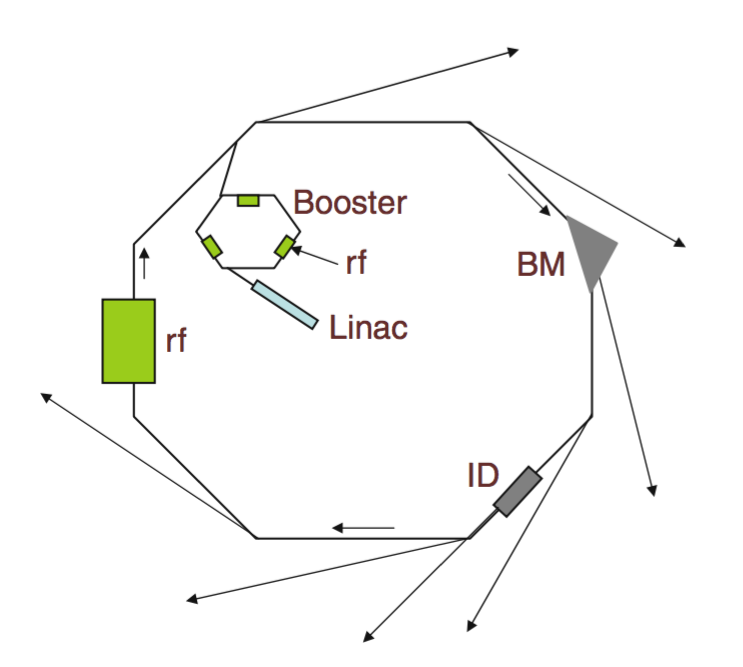
\includegraphics[width=0.7\textwidth]{theory/syn}
	\caption{A schematic representation of a synchrotron radiation source, identifying the Linac, the booster ring, the radio-frequency cavities (rf), the bending magnet (BM) and the insertion device (ID), from Ref \cite{Garcia-Gutierrez2009}.}
	\label{fig:syn}
\end{figure}
%

When an electron accelerates (or travels on a curve), Cherenkov radiation is emitted in accordance with the Cherenkov relation,
%
\begin{equation}
	n_i\beta_c\cos{\theta_e} = 1,
\end{equation}
%
where, $n_i$ is the refractive index for the dielectric medium, $\beta_c$ is the fraction of the speed of light at which that electron is travelling, and $\theta_e$ is the angle between the electron trajectory and the trajectory of the resulting photon.\cite{Garcia-Gutierrez2009} The curve is the result of a bending magnet, meaning that at each bending magnet there can be a beamline which gives out synchrotron light. The light this is given off from a bending magnet is continuous and broad, covering a wide range of the electromagnetic spectrum. The alternative to a bending magnet beamline is a beamline which is served by an insertion device (ID). An insertion device is able to offer more specific radiation characteristics (photon energy, narrower band) than a bending magnet, and are placed on the magnet-free straight sections of the synchrotron. Common insertion devices include wavelength shifters, wigglers, and undulators.

The type of insertion device that is present at both I07 and I22 at DLS is an undulator. An undulator consists of a series of magnets of opposing polarity whihc causes the electrons to `wiggle' back and forth (Figure \ref{fig:undulator}). This results in a superposition of radition from $N_P$ sources, where $N_P$ si the number of magnets, yielding quasi-monochromatic radiation. The brilliance of different X-ray sources are compared in Table \ref{tab:sources}, this shows the significant benefit that an undulator offers in terms of photon brilliance.
%
\begin{figure}
	\centering
	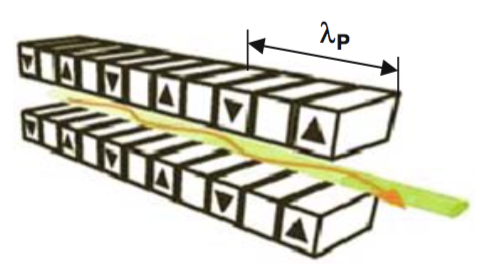
\includegraphics[width=0.7\textwidth]{theory/undulator}
	\caption{A diagram of an undulator insertion device such as that on I07 or I22 where $\lambda_P$ is the period length between opposing magnets, from Ref \cite{Garcia-Gutierrez2009}.}
	\label{fig:undulator}
\end{figure}
%
%
\begin{table}
	\centering
	\caption{A comparision of the photon brilliance from different light sources, adapted from Ref \cite{Sivia2011}.}
	\label{tab:sources}
	\begin{tabular}{l | c}
		\toprule
		\multirow{2}{*}{Light source } & Approximate brilliance/ \\
 & \si{photons\,\second^{-1}\milli\radian^{-2}{0.1}\percent bandwidth^{-1}} \\
		\midrule
		Candle & $10^5$ \\
		X-ray tube & $10^8$ \\
		Sun & $10^{10}$ \\
		Bending magnet & $10^{15}$ \\
		Undulator & $10^{20}$ \\
		\bottomrule
	\end{tabular}
\end{table}

\subsubsection{Neutrons}

Neutrons hold an advantage over X-rays, particularly for application to the study of soft matter, in the ability to utilise contrast variation to increase the quantity of information from the sample, this is discussed in deatil in Section \ref{convar}. However, neutrons cannot be produced safely on a laboratory scale, therefore it is always necessary to visit large scale facilities to harness neutrons for scattering experiments. These facilities come in two flavours; the reactor source and the spallation source, each offering unique benefits.

Neutron reactor sources, such as the Institut Laue-Langevin (ILL) in Grenoble, France, as currently the most common format of neutron source and are capable of producing the highest average neutron flux, the number of neutrons per second per unit area, for example the High-Flux Reactor at the ILL is capable of producing a neutron flux of \SI{1.5E15}{neutrons\,\second^{-1}\centi\meter^{-2}}.\cite{ill2016} A reactor source operates on the principle of nuclear fission, where an atomic nucleus is capable of breaking down into smaller nuclei, overcoming the strong nuclear force. This often involves using uranium enriched with its fissile isotope, \ce{^{235}U}, which after the initial absorption of a stray neutron, from a cosmic ray, or spontaneous fission, will undergo fission to release, on average, 2.5 daughter neutrons, an example of a possible uranium fission mechanism is:
%
\begin{equation*}
	\ce{n + ^{235}U -> ^{236}U -> ^{134}Xe + ^{100}Sr + 2n}.
\end{equation*}
%
This type of mechanism is the basis for research, and nuclear power, reactors.\cite{Sivia2011} One of the major drawbacks for reactor neutron sources is the percieved public opinion towards such facilities. Major saftey concerns, such as ``nuclear meltdown'' and the resulting nuclear waste, mean that reactor souces are often unpopular and therefore struggle to obtain funding required for operation.

The other form of neutron source is a spallation source, this is much less controversial as it does not require fissile materials and hence there is no risk of a nuclear disaster. The ISIS neutron and muon source (Oxfordshire, UK) is an example of a spallation source, where high energy protons, \SI{800}{\mega\eV},\cite{isis2016} are accelerated towards a tungsten target. When the protons strike the target, they can cause the release of a series of neutrons, the first batch of neutrons are given off with too high an energy to be useful, however, less excited neutrons are given off by secondary emissions. In addition to the public preception benefit, spallation sources also have a technological advantage in the time-of-flight technique. The time-of-flight (ToF) technique is based on the fact that at a spallation source, it is possible to know the time at which the neutron was ejected by the target to a high level of precision and accuracy, and therefore it is possible to measure the time taken for the neutron to reach the instrument. Since the neutron is a particle of a finite mass, $m$, it is possible to correlate the velocity, $v$, of the particle with the kinetic energy, $E_k$,
%
\begin{equation}
	E_k = \frac{mv^2}{2},
\end{equation}
%
and with knowledge of the energy of the particle, its wavelength $\lambda$, can be determined by the de Broglie relation,
%
\begin{equation}
	E = h\omega = \frac{hv}{\lambda},
\end{equation}
%
where, $h$ is Planck's constant and $\omega$ is the neutron frequency. Therefore, the wavelength of the neutron is proportional to the inverse of the particle's velocity, and hece the time-of-flight, $t_F$,
%
\begin{equation}
	\lambda = \frac{h}{mv} = \frac{ht_F}{mL_F},
\end{equation}
%
where, $L_F$ is the distance between the target and the instrument. The fact that the neutrons can spread out in the flight from the target means that wavelength-dispersive techniques, where the neutron wavelength is measured rather than the scattering angle, are possible at spallation sources which cannot be carried out at reactor sources. The negative side-effect of current spallation sources is that they have a lower average flux than reactor sources, however the building of the European Spallation Source (ESS) will change this as it offers an average flux similar to that of a reactor source, but with the benefits of the spallation technique.

A problem that is inherent for both reactor and spallation sources is that the energy of the neutrons given off is usually too high to be used to study condensed materials, such as soft matter. This means that moderation must be used to reduce the energy of the neutrons passing through the sample. The neutrons which are considered to be optimal for the study of condensed materials are thermal neutrons, named because their energy is appromately that of ambient temperature. Thermal neutrons are achieved by allowing the neutrons to pass through a large volume of moderator material, usually graphite or heavy water (\ce{D2O}), stored at \SI{300}{\kelvin} before they reach the instrument.\cite{Sivia2011}

\subsection{Contrast variation}
\label{convar}

The scattering profile generated by the interaction of some system with radiation depends on three factors:
%
\begin{itemize}
	\item the spatial arrangement of the atoms in the system,
	\item the instrument being sued to measure the pattern -- instrumental resolution function, and
	\item the interaction between the radiation and the matter under investigation.
\end{itemize}
%
This final factor is perhaps better known as the `scattering contrast', this is an extremely important factor in the study of soft matter, particularly when the probing radiation is the neutron. The scattering contrast makes it possible to select individual components of the system and investigate their structural properties.\cite{Schurtenberger2002} The differential cross-section, $\sfrac{\text{d}\sigma}{\text{d}\Omega}$ of a point scatterer, as shown in Eqn. \ref{equ:sca}, varies only with respect to the scattering length of the species, $b$,
%
\begin{equation}
	\frac{\text{d}\sigma}{\text{d}\Omega} \propto b^2.
\end{equation}
%
However, as discussed in Section \ref{sec:sld}, it is often easier to use the scattering length density, $\rho$.

When an X-ray interacts with an atom, it is scattered by the interaction with the electrons, this is due to the X-ray being a form of electromagnetic radiation. Furthermore, it means that the scattering length of an atom by an X-ray is directly proportional to the number of electrons in the atom, so it is therefore difficult to discern between the scattering from a carbon atom (6 electrons) and a nitrogen atom (7 electrons), furthermore the scattering from hydrogen atoms is practically non-existent.

The scattering length a neutron by an atom varies unsystematically with respect to the atomic number of a species, this is shown in Figure \ref{fig:scatlen}. Furthermore to the apparently random variation with changes in atomic number, there is also significant variation with mass number, e.g. between isotopes of the same atom. This is also dependance due to the magnetic state of the atom, however this is normally unimportant for soft matter. The scattering lengths differ with the nuclear spin energy level, this leads to an average scattering length, $\langle b \rangle$, for isotopes where the nuclear spin is non-zero ($S\neq 0$). There are two forms of scattering, coherent and incoherent, for which the scattering cross-sections, $\sigma$, are determined by,
%
\begin{equation}
	\begin{aligned}
		\sigma_{\text{coh}} & = 4\pi\langle b \rangle ^2 \\
		\sigma_{\text{incoh}} & = 4\pi(\langle b ^ 2 \rangle - \langle b \rangle ^2) \\
	\end{aligned}
\end{equation}
%
The coherent scattering is the scattering from nuclei that all have the same value of $\langle b \rangle$, and leads to the important scattering pattern. Whereas, the incoherent scattering is caused by the `disorder' between the isotopes, and is the cause of the background present in the measurement. Examples of these scattering cross-sections for nuclei relevant to soft matter are shown in Table \ref{tab:crosssec}. It can be seen that the incoherent scattering from the \ce{^1H} nuclei is more than forty times the coherent scattering. This leads to a large, intrusive background present in the scattering pattern of hydrogenous samples.
%
\begin{figure}
	\centering
	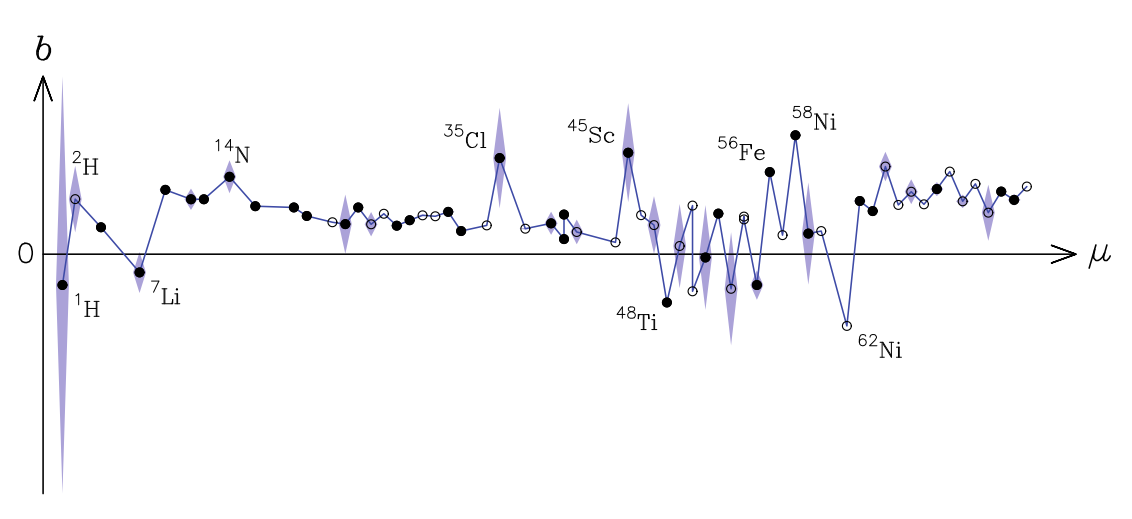
\includegraphics[width=0.7\textwidth]{theory/scatlen}
	\caption{The variation of the average neutron scatteirng length, $\langle b \rangle$ (circles), with atomic mass, $\mu$. The standard deviation, $\Delta b$, is indicated with the shaded regions, from Ref \cite{Sivia2011}.}
	\label{fig:scatlen}
\end{figure}
%
\begin{table}
	\centering
	\caption{Examples of coherent and incoherent scattering cross-sections, from Ref \cite{Schurtenberger2002}.}
	\label{tab:crosssec}
	\begin{tabular}{r | c c c}
		\toprule
		Isotope & $S$ & $\sigma_{\text{coh}}$/\SI{e-28}{\meter\square} & $\sigma_{\text{incoh}}$/\SI{e-28}{\meter\square} \\
		\midrule
		\ce{^1H} & $\sfrac{1}{2}$ & 1.8 & 79.7 \\
		\ce{^2H} & 1 & 5.6 & 2.0 \\
		\ce{^{12}C} & 0 & 5.6 & -- \\
		\ce{^{14}N} & 1 & 11.6 & 0.3 \\
		\ce{^{16}O} & 0 & 4.2 & -- \\
		\bottomrule
	\end{tabular}
\end{table}
%
The difference between the scattering of \ce{^1H} and \ce{^2H}, evident in Table \ref{tab:crosssec}, can lead to a very useful technique if soft matter scattering, known as contrast variation. The idea of contrast variation is based on the substitution of one isotope of an atom for another, while not introducing significant change to the properties of the material. Traditionally the benefit of this came in terms of contrast matching out a part of the system to reduce the dimensionality of the problem for analysis. For example, by matching the solvent scattering length density to that of the tails of the surfactants at the centre of a micelle there would only be scattering from the heads, and conversely there would only be scattering from the tails if the solvent had the same scattering length density as the head groups. This means that the problem becomes more straightforward as there are fewer variable parameters when fitting the data. This idea is represented graphically in Figure \ref{fig:convar}.
%
\begin{figure}
	\centering
	
\includegraphics[width=0.7\textwidth]{theory/convar}
	\caption{The effect of varying the scattering length density of the solvent in a micelle system, (a) the system in pure solvent, (b) the solvent is contrast matched to the surfactant tails, and (c) the solvent is contrast matched to the surfactant heads.}
	\label{fig:convar}
\end{figure}
%
The technique of contrast variation may also be used in terms of data analysis. By increasing the number of data sets corresponding to a single model -- at different constrasts, the solution for the true sturcture of the model from the scattering data becomes more robust. This is due to the fact that each different contrast can be considered as an independent measurement of the same system, and hence each set of scattering data can be used within the data analysis procedure to obtain the best global agreement to the experiment. This co-refinement of multiple experiments can, under the right conditions, be used to simulatenously consider both neutron and X-ray datasets.\cite{Nelson2006}

There is also the possibility of using contrast variation when the probing radiation is the X-ray, through the use of anomalous scattering. This is where different wavelengths of radiation give different scattering, when the wavelengths are on opposite sides on an X-ray absorption edge. This is not frequenctly used for soft matter species, as the X-ray absorption edges for elements common in soft matter (H, C, N, O, etc.) are at very low X-ray energies so generally outside of the accessible range. \cite{Schurtenberger2002}

%\section{Scattering}
\label{sec:scattering}

The use of scattering techniques to probe soft condensed matter systems is commonplace.
In this work, we have focussed on the use of small angle scattering (SAS), reflectometry, and grazing incidence small angle scattering (GiSAS) techniques.
These are particularly appropriate for application to soft condensed matter systems due to the length scales capable of being probed being similar to the persistence length of the soft condensed matter systems.
The length scale covered for such techniques is from around \SI{1}{\nano\metre} to \SI{300}{\nano\metre}, as is shown in Figure~\ref{fig:lengths}.
The focus is on the equilibrium structure(s) of a material, and therefore there is no interest in the system dynamics, meaning that exclusively elastic scattering techniques may be used, where there is no energy transfer between the probing radiation and the material.
This is in contrast to inelastic scattering where energy transfer occurs; facilitating the measurement of system dynamics, such as the dynamical modes of polymers and lipid bilayers \cite{garcia_sakai_quasielastic_2009, farago_recent_2009}.
%
\begin{figure}
    \centering
    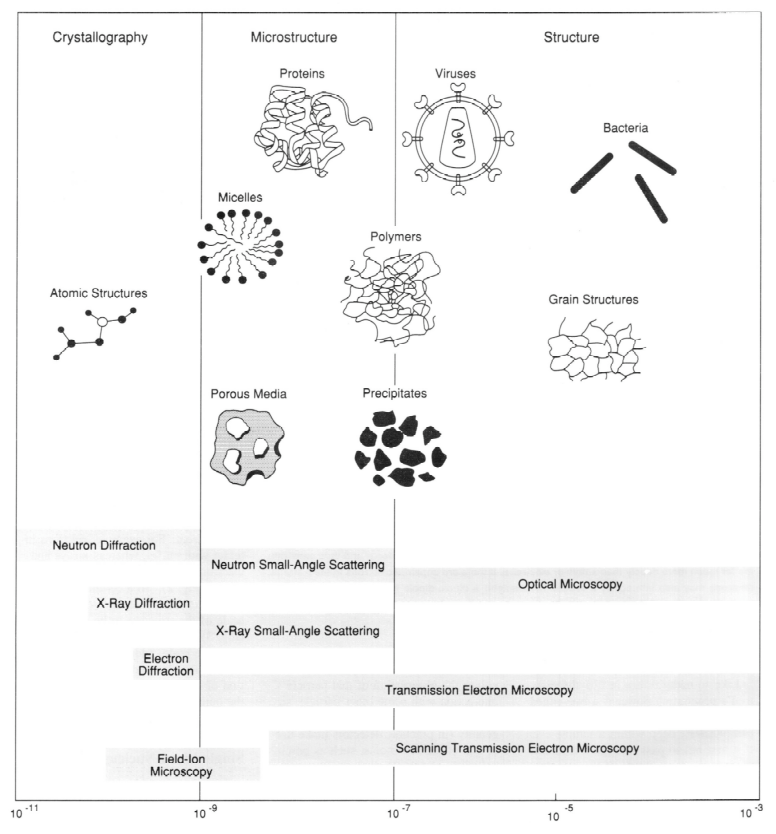
\includegraphics[width=0.85\textwidth]{theory/length}
    \caption{A representation of how different techniques can be used to probe various length scales. Reproduced, with permission of Oxford University Press\textsuperscript{\textcopyright}, from Reference~\cite{sivia_elementary_2011}.}
    \label{fig:lengths}
\end{figure}
%

Both X-ray and neutron scattering techniques are discussed and used in this work.
From an experimental viewpoint, there are significant differences between an X-ray scattering and a neutron scattering experiment.
However, there is little variation in terms of the data analysis, where the differences are limited to; the nature of the scattering lengths, and the higher background that is present in the neutron scattering experiments.

\subsection{The scattering vector}

The scattering of some probing radiation, by some sample, can be represented as shown in Figure~\ref{fig:scat}.
Since only elastic scattering is being considered, there will be no change in the frequency of the radiation, $\omega_i = \omega_f$.
This means that only the wavevector, $\mathbf{k}$, can change, $\mathbf{k}_i\neq \mathbf{k}_f$.
The difference between the incident and final wavevectors is the scattering vector, $\mathbf{q}$, where,
%
\begin{equation}
    \mathbf{q} = \mathbf{k}_i - \mathbf{k}_f.
\end{equation}
%
%
\begin{figure}
    \centering
    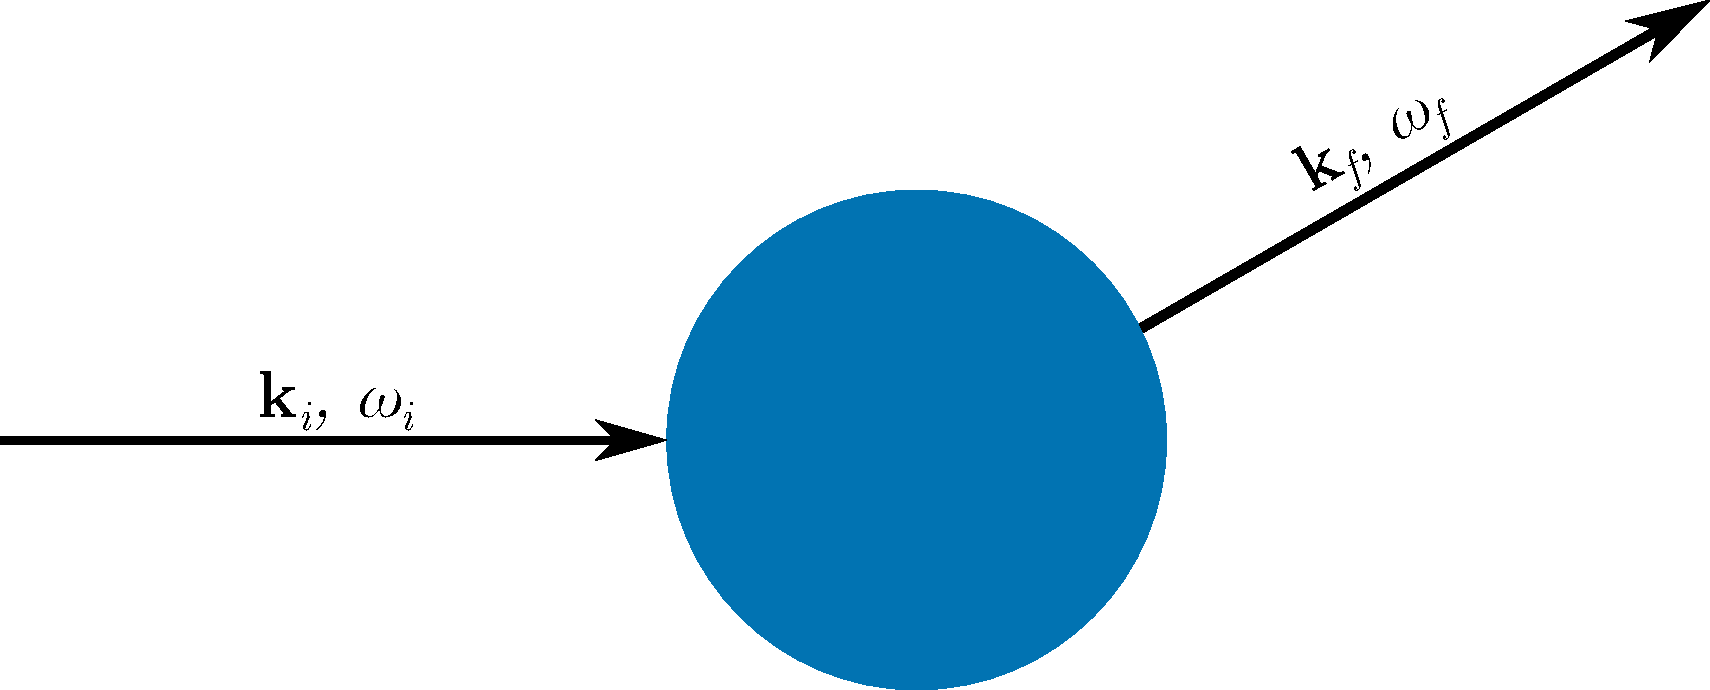
\includegraphics[width=0.85\textwidth]{theory/scat}
    \caption{A schematic of the scattering of some probing radiation by a sample (blue circle). Adapted, with permission of Oxford University Press\textsuperscript{\textcopyright}, from Reference~\cite{sivia_elementary_2011}.}
    \label{fig:scat}
\end{figure}
%
The scattering vector strictly has units of \si{\per\meter}, however it is often more practical to use \si{\per\nano\meter} or \si{\per\angstrom}.
Throughout this work, units of reciprocal \AA ngstrom will be wherever possible.
Since the frequency of the probing radiation does not change during an elastic scattering event, the wavelength, $\lambda$, will also not change, meaning that the moduli of the incident and final wavevectors are,
%
\begin{equation}
    |\mathbf{k}_i| = |\mathbf{k}_f|=\frac{2\pi}{\lambda}.
    \label{equ:wavevec}
\end{equation}
%
This means that only the angle will change during the elastic scattering event.
The vector diagram in Figure~\ref{fig:scatvec} can be used to describe the geometry of an elastic scattering event.
From this, and Equation~\ref{equ:wavevec}, the value of $q$, where $q = |\mathbf{q}|$ can be shown as,
%
\begin{equation}
    q = \frac{4\pi\sin{\theta}}{\lambda}.
    \label{equ:theq}
\end{equation}
%
%
\begin{figure}
    \centering
    \includegraphics[width=0.85\textwidth]{theory/scatvec}
    \caption{A vector diagram describing an elastic scattering event. Adapted, with permission of Oxford University Press\textsuperscript{\textcopyright}, from Reference~\cite{sivia_elementary_2011}.}
    \label{fig:scatvec}
\end{figure}
%
However, this fails to fully capture the three dimensional nature of the scattering event.
Hence, it is necessary to describe the scattering with spherical coordinates, $2\theta$, and $\phi$, such that the incoming and outgoing radiation can be described as,
%
\begin{equation}
    \begin{aligned}
        \mathbf{k}_i & = \bigg(0, 0, \frac{2\pi}{\lambda}\bigg), \\
        \mathbf{k}_f & = \frac{2\pi}{\lambda}(\sin{2\theta}\cos{\phi}, \sin{2\theta}\sin{\phi}, \cos{2\theta}),
    \end{aligned}
\end{equation}
%
where, $|\mathbf{k}_f| = \sfrac{2\pi}{\lambda}$. This allows the scattering vector to be written,
%
\begin{equation}
    \mathbf{q} = \frac{4\pi\sin{\theta}}{\lambda}(-\cos{\theta}\cos{\phi}, -\cos{\theta}\sin{\phi},\sin{\theta}).
\end{equation}
%
For an isotropic scattering pattern, it is the magnitude of the scattering vector, $q$, that is measured.
In practical terms, the scattering vector allows for easy comparison of measurements made at different radiation wavelengths.

The basic quantity measured in a scattering experiment is the differential cross section, $\sfrac{\text{d}\sigma(q)}{\text{d}\Omega}$.
This is the fraction of particles of probing radiation that is scattered with a particular set of polar coordinates, $2\theta$ and $\phi$,
%
\begin{equation}
    \frac{\text{d}\sigma(q)}{\text{d}\Omega} = \frac{R(2\theta,\phi)}{NV\Phi\Delta \Omega},
    \label{equ:dsc}
\end{equation}
%
where, $R(2\theta,\phi)$ is the rate of arrival of the scattered particles at the position $2\theta$, $\phi$, $V$ is the illuminated volume of the sample, $\Phi$ is incident flux, $\Delta \Omega$ is some small solid angle, and $N$ is the number of scattering particles of interest, in the case of elastically scattered radiation, $N = N\%_{\text{el}}$, where $\%_{\text{el}}$ is the fraction of elastically scattered radiation.

\subsection{Scattering from a single fixed particle}

It is possible to describe a steady stream X-ray photons or neutrons of wavelength, $\lambda$, travelling through space as follows,
%
\begin{equation}
    \psi_i = \psi_o \exp{(\mathbf{i} kz)},
    \label{equ:wave}
\end{equation}
%
where, $z$ is the direction of travel, and the incident flux is the magnitude of the wave squared, $\Phi = |\psi_o|^2$.
This wave then interacts with a single fixed particle elastically, propagating the wave radially outwards (Figure~\ref{fig:singleatom}).
This propagation is centred on the atom, therefore the wavevector, $\mathbf{k_f}$ is parallel to the displacement vector, $\mathbf{r}$, and the following holds,
%
\begin{equation}
    \exp{(\mathbf{i}\mathbf{k}_f\cdot \mathbf{r})} = \exp{(\mathbf{i}kr)}.
\end{equation}
%
This final wave is no longer collimated and therefore diminishes with distance, $r$.
Hence the final scattered wave has the form,
%
\begin{equation}
    \psi_f = \psi_o b\frac{\exp{(\mathbf{i}kr)}}{r},
\end{equation}
%
where, $b$ is the scattering length discussed in Section~\ref{convar}.
%
\begin{figure}
    \centering
    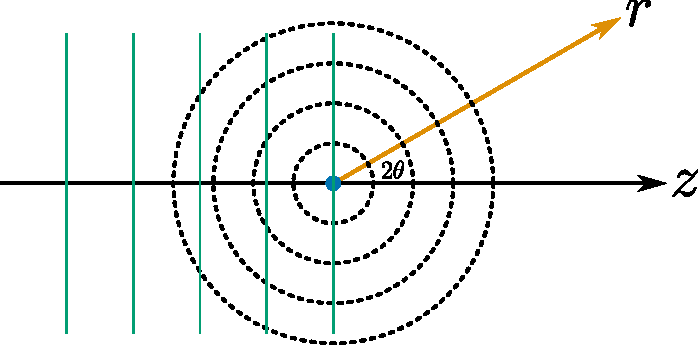
\includegraphics[width=0.85\textwidth]{theory/singleatom}
    \caption{A schematic of the interaction between a single particle and a wave of probing radiation (green lines). Adapted, with permission of Oxford University Press\textsuperscript{\textcopyright}, from Reference~\cite{sivia_elementary_2011}.}
    \label{fig:singleatom}
\end{figure}
%

\subsection{Scattering from multiple particles}
\label{sec:multiscat}

It is important to consider how the probing radiation would interact with a real system, consisting of many particles.
If the incident beam has the form of Equation~\ref{equ:wave}, with the wavevector $\mathbf{k}_i = (0, 0, k)$, each particle, $j$, will contribute the following to the total scattered wave, $psi_f$, made up of the scattering from all, $N$, atoms,
%
\begin{equation}
    [\delta\psi_f]_j = \psi_o\exp{(\mathbf{ik}_i\cdot \mathbf{R}_j)}b_j\frac{\exp{\big\{\mathbf{ik}_f\cdot (\mathbf{r}-\mathbf{R}_j)\big\}}}{|\mathbf{r}-\mathbf{R}_j|},
\end{equation}
%
where, $\mathbf{R}_j$ is the position of particle $j$, $\mathbf{r}$ is some arbitrary position, and $\mathbf{k}_f$ is the wavevector of the scattered wave (Figure~\ref{fig:multiatom}).
This allows the total scattered wave to be defined as a summation of the contributions from the individual waves,
%
\begin{equation}
    \psi_f = \psi_o \exp{(\mathbf{ik}_f\cdot\mathbf{r})}\sum_{j=1}^{N}\bigg\{b_j \frac{\exp{(\mathbf{iq}\cdot \mathbf{R}_j)}}{|\mathbf{r}-\mathbf{R}_j|}\bigg\}.
    \label{equ:scatter}
\end{equation}
%
Equation~\ref{equ:scatter} holds true, within the Born approximation, where the scattered wave has no impact on the incident wave and each wave is scattered only once.
%
\begin{figure}
    \centering
    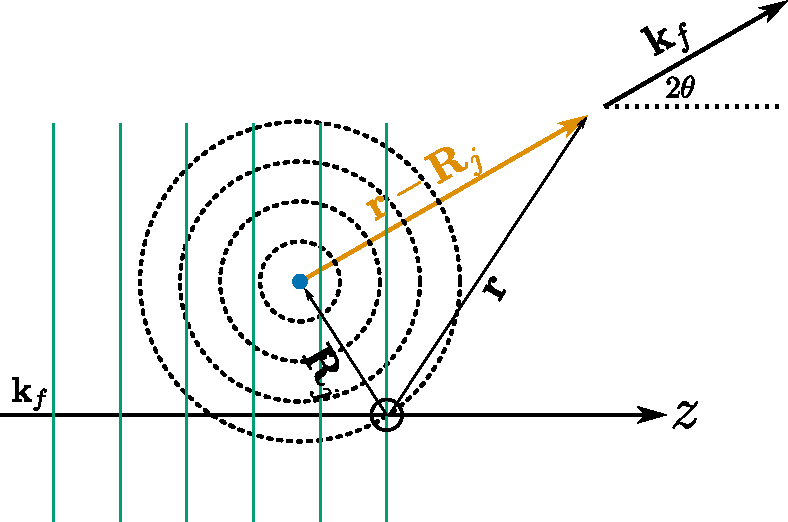
\includegraphics[width=0.85\textwidth]{theory/multiatom}
    \caption{A schematic of the interaction between a particle, $j$, at position $\mathbf{R}_j$ and a wave of probing radiation (green lines). Adapted, with permission of Oxford University Press\textsuperscript{\textcopyright}, from Reference~\cite{sivia_elementary_2011}.}
    \label{fig:multiatom}
\end{figure}
%

The sample-detector distance is usually much larger than the typical particle size, allowing for the following approximation,
%
\begin{equation}
    |\mathbf{r} - \mathbf{R}_j| = |\mathbf{r}| = r.
\end{equation}
%
This is termed the Fraunhofer, or far-field limit, and allows Equation~\ref{equ:scatter} to be simplified,
%
\begin{equation}
    |\psi_f|^2 = \frac{\Phi}{r^2}\Bigg|\sum_{j=1}^{N}b_j\exp{(\mathbf{iq}\cdot\mathbf{R}_j)}\Bigg|^2.
\end{equation}
%
In the scattering experiment, radiation is deflected elastically into a detector with a small area, $\delta A$, with the polar coordinates, $2\theta$ and $\phi$, at a rate of $R_{\text{el}}$,
%
\begin{equation}
    R_{\text{el}}(2\theta,\phi) = |\psi_f|^2\delta A = \Phi\delta\Omega\Bigg|\sum_{j=1}^{N}b_j\exp{(\mathbf{iq}\cdot\mathbf{R}_j)}\Bigg|^2,
\end{equation}
%
where, $\delta\Omega = \sfrac{\delta A}{r^2}$.
Therefore, the differential cross section, defined in Equation~\ref{equ:dsc} can be related to the scattering from the sample as,
%
\begin{equation}
    \bigg(\frac{\text{d}\sigma(q)}{\text{d}\Omega}\bigg)_{\text{el}} = \frac{1}{V} \Bigg|\sum_{j=1}^{N}b_j\exp{(\mathbf{iq}\cdot\mathbf{R}_j)}\Bigg|^2.
    \label{equ:sca}
\end{equation}
%

\subsection{Scattering length density}
\label{sec:sld}

While it may be helpful to consider the scattering of multiple particles individually, where each particle has a scattering length, $b$.
In practice, due to the low experimental resolution at small angles, it is more common to consider the scattering length density, $\rho$, of the system,
%
\begin{equation}
    \rho = \frac{1}{V}\sum_{i=0}^{N} b_i,
\end{equation}
%
where $N$ is the total number of particles in the volume $V$.
A result of this equation is the ability to rewrite Equation~\ref{equ:sca} as,
%
\begin{equation}
    \bigg(\frac{\text{d}\sigma(q)}{\text{d}\Omega}\bigg)_{\text{el}} = \frac{1}{V} \Bigg|\iiint \limits_V \rho\exp{(\mathbf{iq}\cdot\mathbf{R})}\text{d}^3\mathbf{R}\Bigg|^2.
    \label{equ:sldsca}
\end{equation}
%
This above equation shows that the scattering differential cross-section from some object is related to the scattering length density profile of that object by a Fourier transform.

\subsection{Model-dependent analysis}

All types of scattering patterns can be analysed by one of two methods; model independent and model-dependent.
The nature of this work means that it will focus on model-dependent analysis methods, often where the model is derived from some atomistic, or coarse-grained simulation. Model-dependent analysis has significant benefits over model-independent methods, such as improved resolution and more detailed information about the structure.
However, the necessity of the inclusion of \emph{a priori} information within model-dependent analysis may act to bias the result.
While this is undesirable, these assumptions can, and should, be educated based on the chemical information present, such as the propensity for twin-tailed lipid molecules to form monolayers at an air-water interface \cite{mccluskey_model-dependent_2018}.

The scattering from the model system is determined, using technique specific methods that are discussed in detail in later sections.
This is then compared with the experimental data using some goodness-of-fit metric, the model is then varied to find the best possible model for the data provided using some optimisation algorithm.
In order to accurately reproduce the experimental measurement, it is necessary to include some instrumental resolution function, $res(q)$, in the modelling procedure.
This is instrument-specific, although it may be approximated by convolving the experimental dataset with some Gaussian smearing function, the modelled intensity can then be determined from,
%
\begin{equation}
    I(q) = res(q) * \frac{\text{d}\sigma(q)}{\text{d}\Omega},
\end{equation}
%
where, $\sfrac{\text{d}\sigma(q)}{\text{d}\Omega}$ is the differential cross-section, a measure of the number of scattering particles hitting a given solid angle of the detector.

The aim of model-dependent analysis is to obtain a model for the system which agrees well with the experimentally measured scattering data while producing something that is chemically, and physically relevant.
This means that an optimisation algorithm must be applied to these problems, specific algorithms used in this work are discussed in Section~\ref{sec:mcmc} and \ref{sec:partswarm}.

\subsection{Reflectometry}
\label{sec:refltheory}

Reflectometry involves the interaction of the probing radiation with some interface, from which the radiation is reflected.
The geometry of a reflectometry experiment is shown in Figure~\ref{fig:refgeo}, where the reflectometry instrument is in the horizontal configuration, ideal for the study of liquid interfaces.
Reflectometry measurements give information about the structure perpendicular to the interface, the \emph{z}-dimension in Figure~\ref{fig:refgeo}, and therefore the analysis of reflectometry data is founded on the assumption that the layers will be completely homogenous in the plane of the interface, the \emph{xy}-plane in Figure~\ref{fig:refgeo}.
In reality, since the layers are usually not completely homogeneous, an average is obtained for the area in the radiation beam.
%
\begin{figure}
    \centering
    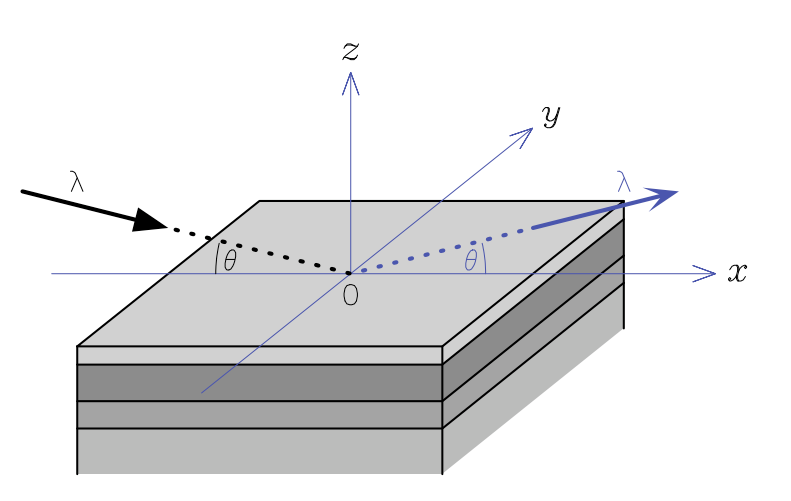
\includegraphics[width=0.85\textwidth]{theory/reflectgeo}
    \caption{A schematic of specular reflectometry from a layered sample. Reproduced, with permission of Oxford University Press\textsuperscript{\textcopyright}, from Reference~\cite{sivia_elementary_2011}.}
    \label{fig:refgeo}
\end{figure}
%
A reflectometry instrument operates by measuring the intensity of specular radiation at a series of different angles, $\theta$, or wavelengths, $\lambda$.
The reflected intensity is defined in terms of $q$ (by Equation~\ref{equ:theq}), and is defined as follows,
%
\begin{equation}
    R(q) = \frac{\text{specular reflected radiation at }q}{\text{incident radiation}}.
    \label{equ:refl}
\end{equation}
%
It is clear from Equation~\ref{equ:refl} that the value of the measured reflectometry cannot be greater than one, as this would mean that more particles of probing radiation were being reflected than were incident.

\subsubsection{Analysis}

There are two model-dependent analysis techniques that can be applied to the rationalisation of a reflectometry dataset.
The first is the kinematic approach, which can be obtained from Equation~\ref{equ:sca}, from the assumption that $q_x = 0$ and $q_y = 0$, as we are only measuring the specular scattering.
This approach models the reflectometry as a function of the scattering length density profile in the \emph{z}-dimension, $\rho(z)$,
%
\begin{equation}
    R(q) \approx \frac{16\pi^2}{q^4}\bigg|\int_{-\infty}^{+\infty}\frac{\text{d}\rho(z)}{\text{d}z}\exp{(-\mathbf{i}zq_z)}\text{d}z\bigg|^2,
    \label{equ:kine}
\end{equation}
%
where, $\sfrac{\text{d}\rho(z)}{\text{d}z}$ is the first derivative of the scattering length density profile.
However, this method has a significant problem, which can be demonstrated by applying Equation~\ref{equ:kine} to the scattering length density profile of a bare silicon substrate, which can be modelled as a Heaviside function (Figure~\ref{fig:kine}a),
%
\begin{equation}
    \rho(z) =
  \begin{cases}
    0, & \text{where}\ z < 0 \\
    \rho_{\text{Si}}, & \text{otherwise}
  \end{cases}
\end{equation}
%
where, $\rho_{\text{Si}}$ is the scattering length density of pure silicon (\SI{2.1e-6}{\angstrom^{-2}} for neutrons).
The derivative of a stepwise Heaviside function is a scaled $\delta$-function (Figure~\ref{fig:kine}b),
%
\begin{equation}
    \rho'(z) = \rho_{\text{Si}}\delta(z).
\end{equation}
%
Then, as in Equation~\ref{equ:kine}, the Fourier transform of this $\delta$-function is taken,
%
\begin{equation}
    \rho_{\text{Si}}\int_{-\infty}^{+\infty}\delta(z)\exp{(-\mathbf{i}zq_z)}\text{d}z = \rho_{\text{Si}}\exp(0) = \rho_{\text{Si}}.
\end{equation}
%
This means that the reflectometry profile could be calculated from the following relationship,
%
\begin{equation}
    R(q)\approx \frac{16\pi^2\rho_{\text{Si}}^2}{q_z^4}.
\end{equation}
%
The curve from this relationship is shown in Figure~\ref{fig:kine}, where it is clear that the agreement with an experimental profile would be poor as $q \rightarrow 0$.
It can be seen that for low values of $q$ the calculated reflectometry is greater than 1, which violates the physical constraint imposed with Equation~\ref{equ:refl}.
This break down of the kinematic approach is due to the assumption present in this approach that the Born approximation (mentioned in Section~\ref{sec:multiscat}) will hold.
However, in the reflectometry scattering geometry, this is no longer true rendering the kinematic approach invalid.
%
\begin{figure}
    \centering
    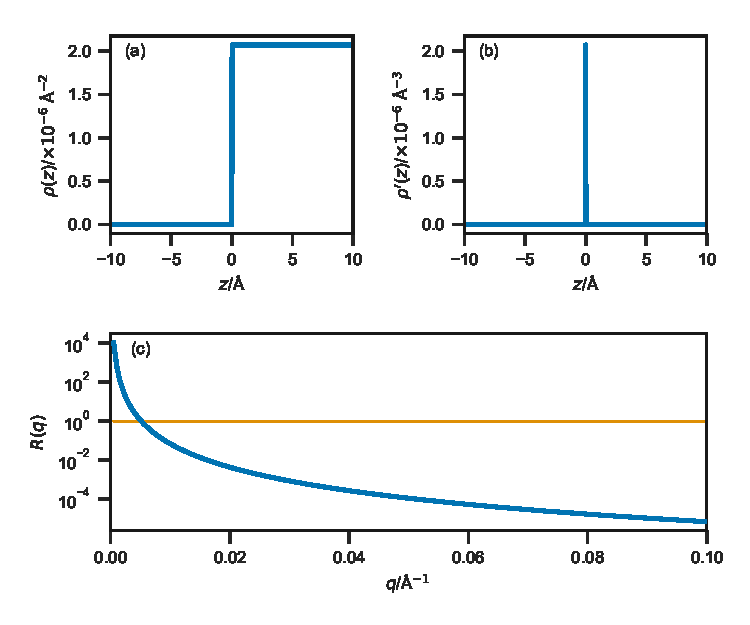
\includegraphics[width=0.85\textwidth]{theory/kine}
    \caption{A graphical representation of the kinematic approach; (a) the Heaviside function describing the scattering length density profile of a bare silicon substrate, (b) the $\delta$-function arising from the first derivative of the function in (a), and (c) the reflectometry profile resulting from Equation~\ref{equ:kine}, where the orange line at $R=1$ identifies the break down between experimental and theory in the kinematic approach. Adapted, with permission of Oxford University Press\textsuperscript{\textcopyright}, from Reference~\cite{sivia_elementary_2011}.}
    \label{fig:kine}
\end{figure}
%

This breakdown of the kinematic approach has led to the application of the Abel\`{e}s, or Parratt, model for the reflection of light at a given number of stratified interfaces (also known as dynamical theory) \cite{abeles_sur_1948,parratt_surface_1954}.
This method involves considering the system as a layered structure at the interfaces of which the probing radiation can either be reflected or refracted, by some refractive index, $n_i$.
Figure~\ref{fig:reflrefr} shows this process for a system of two layers, where the layer $0$ is the air or vacuum above the sample, it is clear to see how the two waves labelled $r$ could interfere constructively or destructively depending on the thickness of layer $1$, $d$.
This means that for a single interface, such as that between layers $0$ and $1$ in Figure~\ref{fig:reflrefr}, the reflectometry can be described by the Fresnel equation,
%
\begin{equation}
    R(q) = \bigg| \frac{n_0\sin{\theta_0} - n_1\sin{\theta_1}}{n_0\sin{\theta_0} + n_1\sin{\theta_1}} \bigg|^2.
\end{equation}
%
Additionally at the point of total reflection, where $\theta_0 = \theta_{\text{c}}$, the critical angle, there will be no transmitted wave so,
%
\begin{equation}
    n_1\sin{\theta_1} = 0,
\end{equation}
%
and therefore the reflected radiation will never be greater than 1, while the critical angle can be defined as,
%
\begin{equation}
    \cos^2{\theta_{\text{c}}} = \frac{n_1^2}{n_0^2}.
\end{equation}
%
This is the angle below which a reflectometry profile will be measured.
%
\begin{figure}
    \centering
    \includegraphics[width=0.85\textwidth]{theory/reflrefr}
    \caption{A schematic diagram showing the reflected ($r$) and transmitted ($t$) waves when an incident ($i$) wave enters an interface of thickness $d$, where the refractive indices of each layer are $n_0$, $n_1$, and $n_2$. Adapted from \cite{foglia_studies_2015}, with permission from Elsevier.}
    \label{fig:reflrefr}
\end{figure}
%

The above method can then be generalised to a structure of an arbitrary number of layers, as shown in Code Block~\ref{cb:refl}.
For each value of $q$ for which the reflectometry is to be calculated, the system is considered in terms of $n_{\text{max}}$ layers.
The incident radiation beam will be refracted by each of the layers, giving wavevectors values for each layer, $k_n$,
%
\begin{equation}
    k_n = \sqrt{k_0^2 + 4\pi (\rho_n - \rho_0)},
\end{equation}
%
where, $k_0=\sfrac{q}{2}$.
The Fresnel equation coefficient between layers $n$ and $n+1$, $r_{n,n+1}$ can then be found along with the phase factor, $\beta_n$, which is dependent on the thickness of the layer, $d_n$,
%
\begin{equation}
    r_{n,n+1} = \frac{k_n - k_{n+1}}{k_n + k_{n+1}},
    \label{equ:fres}
\end{equation}
%
%
\begin{equation}
    \beta_n = k_n d_n.
\end{equation}
%
The means that a matrix can be evaluated for each layer, $M_n$,
%
\begin{equation}
    M_n =
    \begin{bmatrix}
        \exp{\beta_n} & r_{n,n+1}\exp{-\beta_n} \\ r_{n,n+1}\exp{\beta_n} & \exp{-\beta_n}
    \end{bmatrix}
\end{equation}
%
The resultant matrix, $B_n$, is then found as a product of the matrix from each layer,
%
\begin{equation}
    B = \prod_{n=0}^{n_{\text{max}}} M_n,
\end{equation}
%
and from this the reflected intensity at the given value of $q$ can be found,
%
\begin{equation}
    R(q_z) = \frac{B_{1,2}}{B_{1,1}}.
\end{equation}
%
This algorithm models the layers as perfectly flat layers, which will not be strictly true in the case of soft matter systems such as a bilayer.
This resulted in the correction term being added to Equation~\ref{equ:fres} to account for the roughness of the layers.
This adapts Equation~\ref{equ:fres} to the form,
%
\begin{equation}
    r_{n,n+1} = \frac{k_n - k_{n+1}}{k_n + k_{n+1}}\exp{(-2k_nk_{n+1}\sigma^2_{n,n+1})},
\end{equation}
%
where, $\sigma_{n,n+1}$ is the interfacial roughness between layers $n$ and $n+1$.
This has the effect of Gaussian broadening the layers into each other, as a result. Code Block~\ref{cb:refl} is currently implemented in a variety of reflectometry modelling software packages, such as \texttt{refnx}, MOTOFIT, RasCAL, and Aurore \cite{nelson_refnx_2019,nelson_co-refinement_2006,hughes_rascal_2010,gerelli_aurore_2016-1,gerelli_aurore_2016}.
Applying this method to the scattering length density profile shown in Figure~\ref{fig:kine} gives the reflectometry profile shown with the dashed green line in Figure~\ref{fig:dyna}.
%
\begin{figure}
    \centering
        \lstinputlisting[caption={An example code block for the Abel\`{e}s method for the calculation of reflectometry, adapted from Reference~\cite{nelson_refnx_2019}.},label={cb:refl}]{reports/code_blocks/reflectometry.py}
\end{figure}
%
%
\begin{figure}
    \centering
    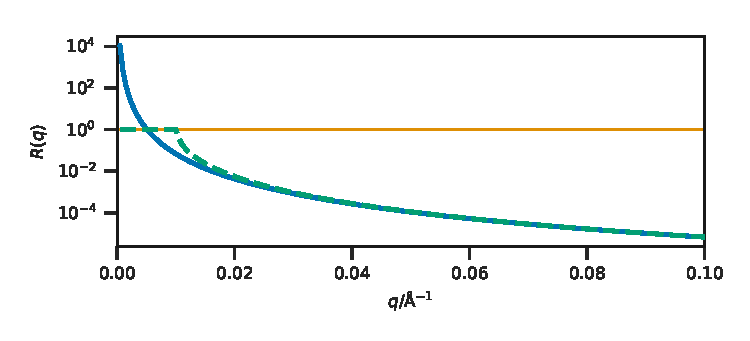
\includegraphics[width=0.85\textwidth]{theory/dyna}
    \caption{A comparison of the kinematic approach (blue solid line), and the dynamical approach (green dashed line), to determine the reflected intensity from the material with the scattering length density profile given in Figure~\ref{fig:kine}(a). It is clear that at low $q$, there is a noticable deviation between the two.}
    \label{fig:dyna}
\end{figure}
%


\subsection{Small angle scattering}

Equation~\ref{equ:sldsca} identified that the scattering differential cross-section for some object was related to the scattering length density by a Fourier transform, which is shown graphically in Figure~\ref{fig:scales}.
This figure shows that there is a reciprocal relationship between the size of the object and the scattered intensity, decaying significantly up to values of $2\pi/d_x$, where $d_x$ is the size of the object.
This means that in order to probe the large-scale structural features that are of interest in the study of soft materials, it is necessary to consider small values of $q$.
When considering the nature of $q$ in Equation~\ref{equ:theq}, it is clear that such experiments would benefit from small values of $\theta$ and large values of $\lambda$.
Hence, the application of small angle scattering (SAS).
%
\begin{figure}
    \centering
    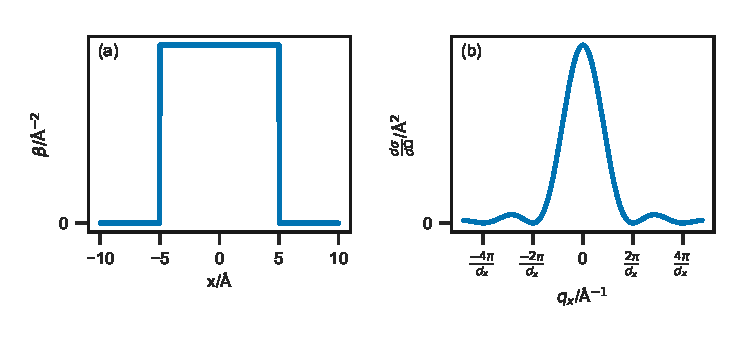
\includegraphics[width=0.85\textwidth]{theory/scales}
    \caption{The effect of a Fourier transform (a) the scattering length density profile for some object with a width of \SI{10}{\angstrom}, (b) the Fourier transform of this object showing the minima in the differential cross section at values of $\sfrac{2n\pi}{10}$, where $n$ is some integer.}
    \label{fig:scales}
\end{figure}
%

A SAS experiment generally involves some sample being placed in the path of the probing radiation; the scattering pattern that results from this transmission is measured at some distance, as is shown in Figure~\ref{fig:sasgeo} for the D22 SANS instrument of the ILL.
SAS instruments are usually very large, due to the large post sample flight path that is necessary to reach the small angles being measured; a longer flight path allows more space for angular divergence.
Transmission SAS can provide information about the size, shape and orientation of the sample's components \cite{willis_experimental_2009}.
The range in $q$ that is typically covered by a SAS instrument is usually around \SIrange{2e-3}{0.5}{\per\angstrom}, which corresponds to \SIrange{10}{3000}{\angstrom} in real-space. The neutron or X-ray detector of a SAS instrument is often two-dimensional, meaning that for an isotropic scattering profile, the detector image is radially averaged to give an $I(q)$ scattering profile.
It is possible to increase the $q$-range of a SAS instrument through the introduction of wide-$q$ detector banks close to the sample or small-$q$ detector banks further away.
This allows the SANS2D instrument, at the ISIS Neutron and Muon Source, to have a total range from \SIrange{2e-3}{2}{\per\angstrom} \cite{noauthor_isis_nodate}.
Furthermore, the SANS2D instrument may leverage the time-of-flight method discussed in Section \ref{sec:neutrons} to allow for a much shorter post sample flight path than is present at D22.
%
\begin{figure}
    \centering
    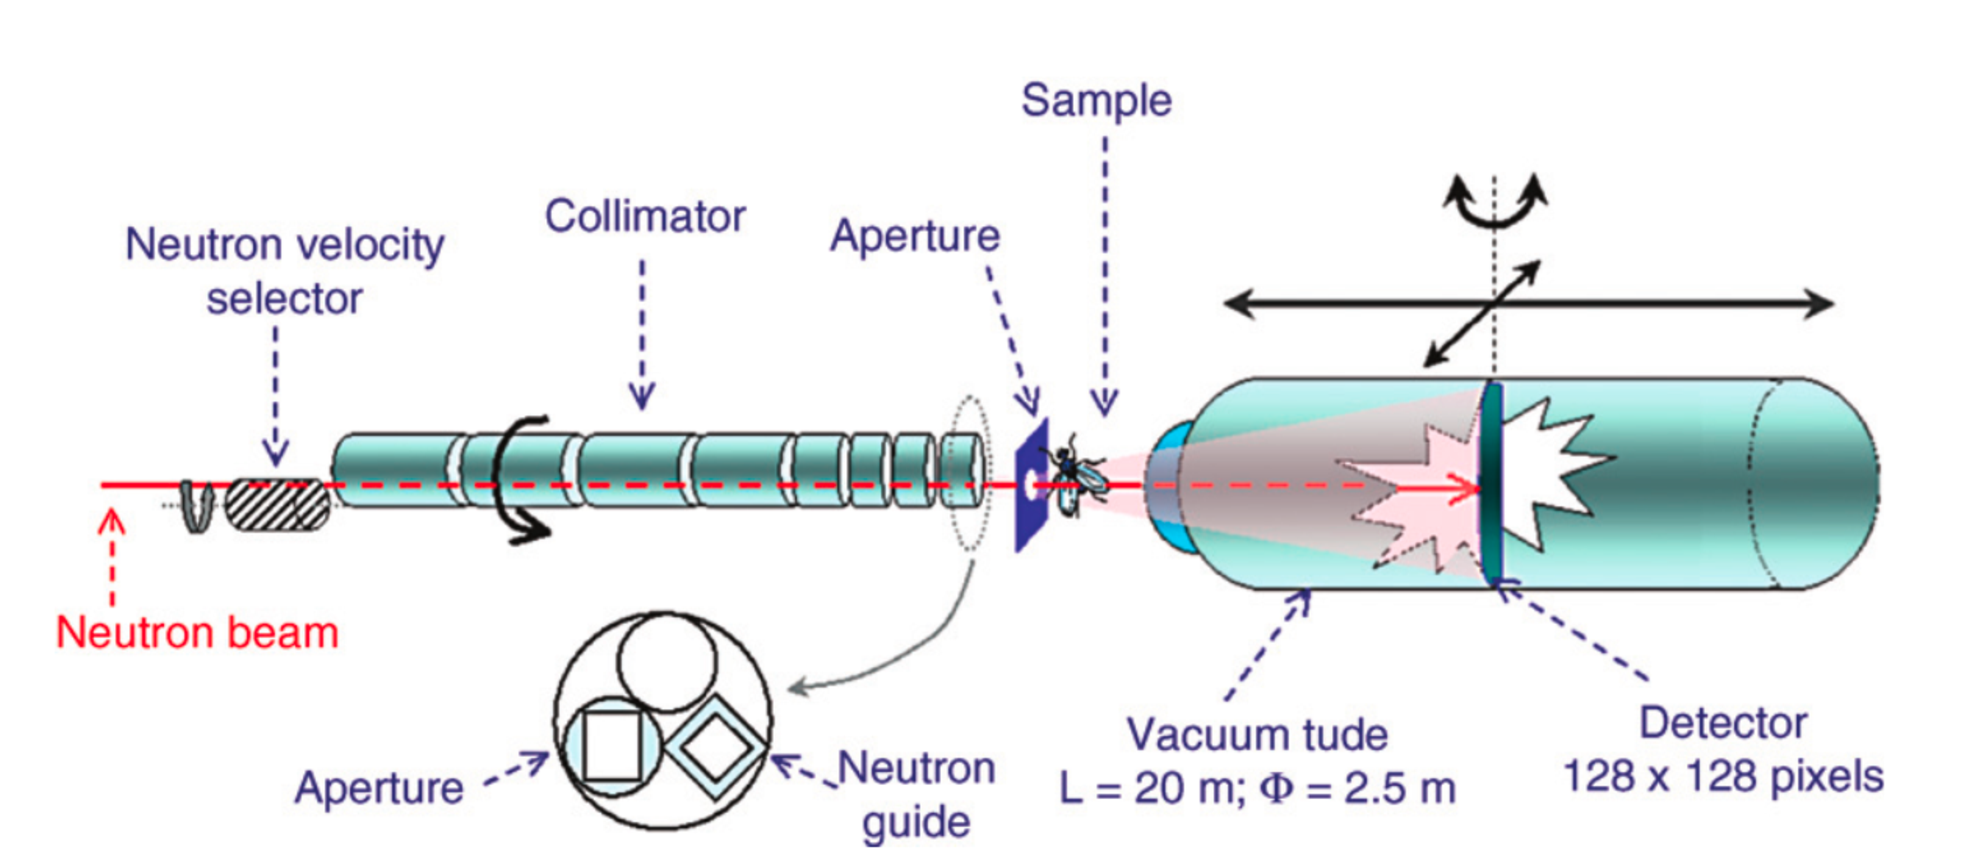
\includegraphics[width=0.85\textwidth]{theory/d22}
    \caption{A schematic of the D22 instrument of the ILL, from Reference~\cite{grillo_small-angle_2008}. Reprinted/adapted by permission from Springer Nature Customer Service Centre GmbH: Springer Nature Small-Angle Neutron Scattering and Applications in Soft Condensed Matter by I. Grillo\textsuperscript{\textcopyright} (2008).}
    \label{fig:sasgeo}
\end{figure}
%

\subsubsection{Analysis}

A radially averaged SAS pattern can be considered as consisting of two sections that arise from the form and structure factors for the scattering species.
The form factor gives information about the average shape of the scattering particle, while the structure factor is a measure of the interaction present between the objects.
It is often possible to control the presence of the structure factor by changing the concentration of the sample, eventually, the concentration will be so low that all interparticle interaction is screened by the solvent \cite{edler_combining_2015}.
This method is frequency applied in BioSAXS applications, where the interactions between the protein molecules are of less interest than the overall structure of the complex.
However, with micelles, it is not always possible to remove the structure factor, as the critical micelle concentration may be higher than the minimum concentration at which the structure factor is present.
It is possible to deconvolute the structure and form factors for a micellar solution by studying different concentrations, assuming that the form of the micelle is concentration independent, over the measured concentration range.

The rigorous, model-independent method for the analysis of SAS involves taking the inverse Fourier transform of the scattering, to give an auto-correlation function of the average particle in the system, which following a deconvolution procedure will resolve the radially averaged scattering length density profile.
However, this is often cumbersome and has a low information density, when compared to model-dependent techniques.
Additionally, if the experimental data lacks information at wide enough $q$ to cover all features of the sample artefacts may be present in the inverse Fourier transform of the scattering.

There are two common and straight-forward analysis procedures that can be used to give an understanding of the scattering species.
The first is the Guinier approximation, which is used in the determination of the radius of gyration, $R_g$, of the scattering species, at ``infinite dilution''.
This scattering law is only valid at very small values of $q$, where $q < R_g^{-1}$ \cite{sivia_elementary_2011},
%
\begin{equation}
    \ln[I(q)] = \ln[I(0)] - \Bigg(\frac{R_g^2}{3}\Bigg)q^2.
\end{equation}
%
This relationship allows the radius of gyration to be found by plotting the scattering profile transformed into $\ln[I(q)]$ vs. $q^2$, and evaluating the gradient at low $q$.
The Guinier plot for the scattering from a sphere with a radius of \SI{20}{\angstrom} is shown in Figure~\ref{fig:rg}, where the radius of gyration correlates with the radius of the sphere, $R$, as follows,
%
\begin{equation}
    R_g = \sqrt{\frac{3}{5}}R.
\end{equation}
%
The Guinier analysis is very common in the study of proteins by SAS, as it allows for the determination of the protein size in the native, solution phase \cite{skou_synchrotron-based_2014}.
Another common analysis of SAS data comes in the form of Porod's law, which states that for large values of $q$, the scattering intensity becomes proportional to $Sq^{-4}$, where $S$ is the surface area of the sample.
This means that by plotting $I(q)q^4$ vs. $q$ and extrapolating to $q \rightarrow \infty$, it is possible to determine the external surface area of the system \cite{willis_experimental_2009}.
Using the surface area it is then possible to qualitatively determine the `roughness' of the system.
%
\begin{figure}
    \centering
    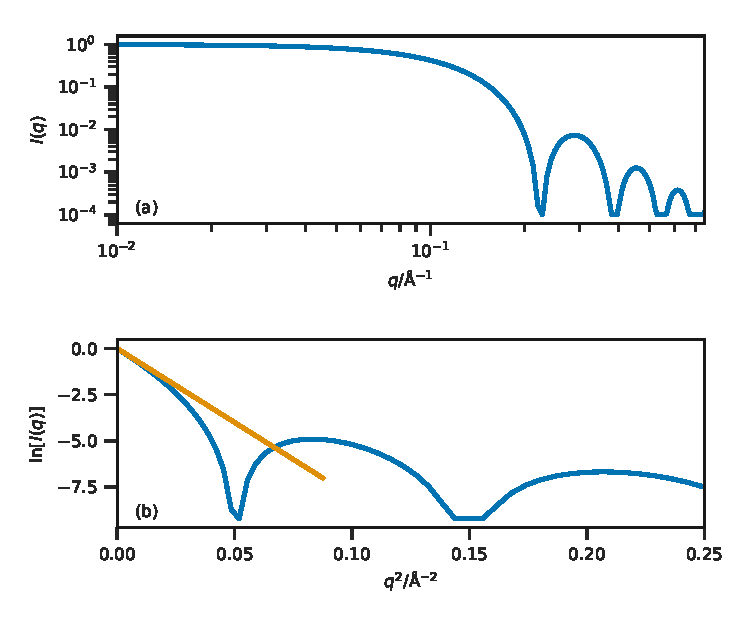
\includegraphics[width=0.85\textwidth]{theory/rg}
    \caption{The Guinier plot, (a) the ideal scattering profile from a sphere of radius \SI{20}{\angstrom}, (b) the associated Guinier plot, with a straight line (orange) at low-$q$ showing the radius of gyration to be \SI{\sim15.5}{\angstrom}.}
    \label{fig:rg}
\end{figure}
%

In the calculation of a SAS pattern, both the structure and form factors will contribute.
Therefore, when we model the pattern, the differential cross-section has the following form, when the system is centrosymmetric.
%
\begin{equation}
    \frac{\text{d}\sigma(q)}{\text{d}\Omega} = N_\rho\Delta\rho^2V_p^2 P(q)S(q),
\end{equation}
%
where $N_\rho$ is the number density of the particles, $\Delta\rho$ is the difference in scattering length density between the particles and the solvent, $V_p$ is the particle volume, $P(q)$ is the particle form factor, and $S(q)$ is the structure factor \cite{pedersen_monte_2002}.
Therefore, it is necessary to understand how the function of the form factor and structure factor come to be.

The most common method for the modelling of the form-factor is by using very coarse shapes; such as spheres, cylinders, or ellipses.
This involves the evaluation of analytical or quasi-analytical solutions for the scattering, which have been derived for many common shapes.
The solution for a sphere was solved in the early 19th century by Lord Rayleigh \cite{pedersen_monte_2002}.
%
\begin{equation}
    P(q) = \Bigg\{\frac{3\big\{\sin(qR) - qR\cos(qR)\big\}}{(qR)^3}\Bigg\}^2,
    \label{equ:sphere}
\end{equation}
%
where $R$ is the radius of the sphere. A comparison between a possible experimental scattering pattern and the scattering generated from Equation~\ref{equ:sphere} is shown in Figure~\ref{fig:sphere}. Analytical form factors exist for a wide variety of shapes; these can be found in software such as SASView and SASFit \cite{noauthor_sasview_nodate, noauthor_sasfit_nodate}.
%
\begin{figure}
    \centering
    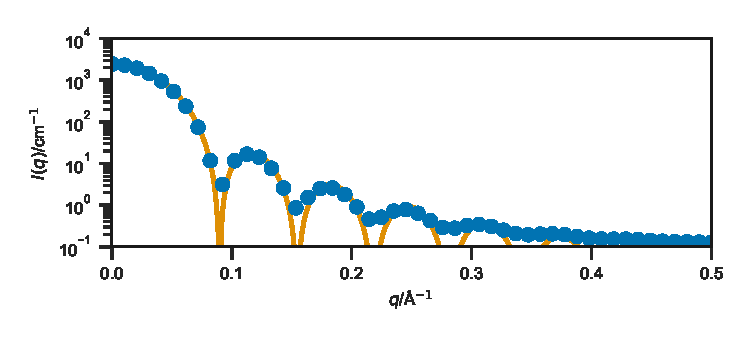
\includegraphics[width=0.85\textwidth]{theory/sphere}
    \caption{The SANS profile of a micelle of \ce{C_{16}TAB} with radius $\SI{50(3)}{\angstrom}$ (circles, generated using SASView \cite{noauthor_sasview_nodate}, with instrumental smearing) compared with a curve of Equation~\ref{equ:sphere}, where $R = \SI{50}{\angstrom}$ (solid line).}
    \label{fig:sphere}
\end{figure}
%

The structure factor accounts for the scattering interference that arises from the interaction of different particles.
This is modelled using expressions which depend on the nature of the scattering particles; hard-sphere, sticky hard-spheres, screened Coulomb, etc.
Structure factor expressions are generated as solutions to the Ornstein-Zernike Equation~\cite{klein_interacting_2002}.
The most relevant structure factor in terms of micelle modelling is probably the Hayter-Penfold Mean Spherical Approximation \cite{hayter_analytic_1981}, this is where the micelles are modelled as like-charged, soft spheres and is valid for dilute solutions.
Again, a whole range of these structure factor functions are built into the SASView package \cite{noauthor_sasview_nodate}.

In order to evaluate the scattering profile from an atomic, or coarse-grained system, it is possible to use the Debye equation \cite{debye_zerstreuung_1915}.
This is an analysis relation for the determination of the scattering profile based on the atomic positions, $\mathbf{r}_i$,
%
\begin{equation}
    I(q) = \sum_{i}^{N}\sum_{j}^{N} b_ib_j\frac{\sin{(q|\mathbf{r}_i-\mathbf{r}_j|)}}{q|\mathbf{r}_i-\mathbf{r}_j|},
\end{equation}
%
where, $N$ is the number of particles, $q$ is the scattering vector, and $b_i$ and $b_j$ are the scattering lengths of particles $i$ and $j$ respectively, for a coarse-grained particle this can be obtained from summing the scattering lengths of the constituent atoms.
The Debye equation is powerful, however, it is not intrinsically parallelisable and as a result scales as $\mathcal{O}(N^2)$.
In order to improve the efficiency of the calculation of the scattering profile, a variety of methods have been developed that offer a sufficiently accurate approximation \cite{svergun_solution_1994,watson_rapid_2013}.
The Golden Vector method, developed by Watson and Curtis \cite{watson_rapid_2013} scales as $\mathcal{O}(Nn)$, where $n$ is the number of scattering vectors used in the calculation.
In this method, the scattering amplitude is calculated numerically for a single $\mathbf{q}$-vector,
%
\begin{equation}
    I(\mathbf{q}) = \Bigg[\sum_{i}^{N}b_i\cos{(\mathbf{q}\cdot\mathbf{r}_i)}\Bigg]^2 + \Bigg[\sum_{i}^{N}b_i\sin{(\mathbf{q}\cdot\mathbf{r}_i)}\Bigg]^2.
\end{equation}
%
This is carried out for $n$ scattering vectors that are selected in an orientationally averaged fashion from a quasi-uniform lattice on a sphere.
This was first developed such that $n$ is a number from the Fibonacci sequence \cite{svergun_solution_1994}, however for the Golden Vector method, $n$ may be any positive integer.
This leads to the scattering vectors being calculated as,
%
\begin{equation}
    \begin{aligned}
        q_x^{(k)} & = q\cos\Bigg[\sin^{-1}\bigg(\frac{2k}{n}\bigg)\Bigg]\cos\bigg(\frac{2\pi k}{\Phi}\bigg), \\
        q_y^{(k)} & = q\cos\Bigg[\sin^{-1}\bigg(\frac{2k}{n}\bigg)\Bigg]\sin\bigg(\frac{2\pi k}{\Phi}\bigg), \\
        q_z^{(k)} & = \frac{2 k q}{n},
    \end{aligned}
\end{equation}
%
where, $k$ runs from $-(n-1)/2,\ldots,0,\ldots,(n-1)/2$ and $\Phi$ is the golden ratio,
%
\begin{equation}
    \Phi = \frac{1+\sqrt{5}}{2}.
\end{equation}
%
The approximate orientationally averaged scattering is then found as an average of the scattering from each of ther individual $q$-vectors,
%
\begin{equation}
    I(q) = \frac{1}{n}\Bigg\{\sum_{k=(1-n)/2}^{(n-1)/2} I[\mathbf{q}^{(k)}]\Bigg\}.
\end{equation}
%
The accuracy of this calculation increases with $n$, however good agreement between experiment and simulation has been shown for $n < 100$ even for highly anisotropic systems \cite{watson_rapid_2013}.


\subsection{Grazing incidence small angle scattering}

While reflectometry is the study of specular reflections from a layer structure, grazing incidence small angle scattering (GISAS) is the study of the off-specular reflections, those where the scattering vector has $x$- and $y$-components in addition to the $z$-component.
This off-specular scattering is that which arises from the heterogeneity present at the interface.
This means that GISAS is ideal for the study of material with nanostructure in the plane of the interface, such as organic semiconducting materials or polymer-grafted nanoparticles at an interface \cite{muller-buschbaum_local_2005,zhang_ion-specific_2017}.
The geometry of a GISAS experiment on a thin film material is shown in Figure~\ref{fig:gisas}, which also shows a typical GISAS pattern.
%
\begin{figure}
    \centering
    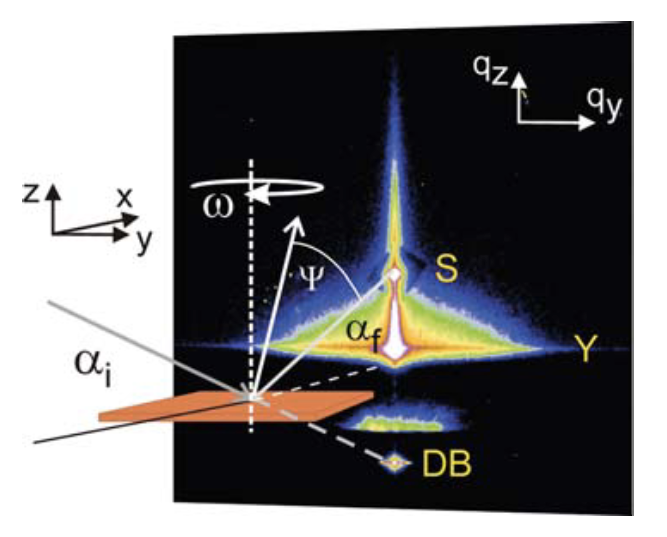
\includegraphics[width=0.85\textwidth]{theory/gisas}
    \caption{A schematic of the geometry of a GISAS experiment, where $\alpha_i$ is the incident angle, $\alpha_f$ is the exit angle, and $\phi$ is the out-of-plane angle, from Reference~\cite{muller-buschbaum_basic_2009}. Reprinted/adapted by permission from Springer Nature Customer Service Centre GmbH: Springer Nature A Basic Introduction to Grazing Incidence Small-Angle X-Ray Scattering by P. M\"{u}ller-Buschbaum\textsuperscript{\textcopyright} (2009).}
    \label{fig:gisas}
\end{figure}
%

In terms of GISAS instrumentation, it can be considered as an amalgamation of a reflectometry instrument and a small angle scattering instrument.
The sample environment is that from a reflectometry instrument, while the two-dimensional detector required is that commonly associated with small angle scattering.
Commonly, GISAS is found as an additional capability of another instrument, such as the grazing incidence small angle neutron scattering (GISANS) capability of D22 at the ILL or the GISAS setup at I07 of the Diamond Light Source \cite{muller-buschbaum_grazing_2004,nicklin_diamond_2016}.
However, as GISAS has grown in popularity as a technique, GISAS focused instruments have been installed, such as MiNaXS at DESY in Hamburg and Beamline 7.3.3 at the ALS in San Francisco \cite{buffet_p03_2012,hexemer_saxs/waxs/gisaxs_2010}.

\subsubsection{Analysis}

The analysis process for a GISAS pattern is substantially more complex than for either the SAS or reflectometry counterparts.
This is due to the fact that for SAS, the Born approximation is conserved, and only a single scattering event is considered.
While for reflectometry, there is a well defined theoretical background that enables the analysis where the Born approximation is not valid.
This is not the case for GISAS since for off-specular reflectometry to occur, the probing radiation will undergo both scattering and reflectometry events simultaneously.
In order to account for this, generally, the distorted wave Born approximation (DWBA) is invoked.
This is an extension of the Born approximation, wherein there are four possible ways in which the probing radiation may interact with the material, these are shown in Figure~\ref{fig:dwba}.
%
\begin{figure}
    \centering
    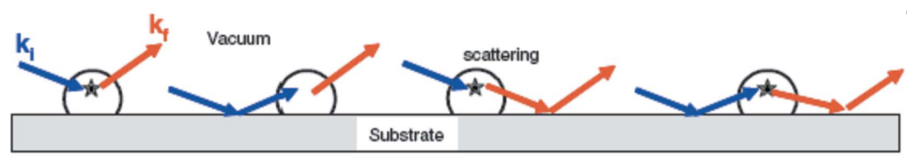
\includegraphics[width=0.85\textwidth]{theory/dwba}
    \caption{The four possible way in which some probing radiation may interact with a sample within the DWBA; scattering, reflection-then-scattering, scattering-then-reflection, and reflection-then-scattering-then-reflection, from Reference~\cite{hexemer_advanced_2015}.}
    \label{fig:dwba}
\end{figure}
%

One of the most common methods for the analysis of a GISAS pattern is Bragg peak analysis.
This is where Bragg peaks of crystallinity in the GISAS pattern are selected and analysed in terms of Bragg's and Snell's laws to account for the effects of the surface and substrate, this allows the dependence of $q_z$ to be determined \cite{lee_electron_2007, busch_grazing-incidence_2006}.
While useful, this analysis approach is limited to systems with high crystallinity, such as stacked lamellae \cite{busch_inner_2007}.
This method cannot be easily applied to understand less organised arrangements in soft matter systems, as these give rise to broad, smeared peaks with no clear centre.

Another simplified method for the analysis of a GISAS pattern involves the effective surface approximation.
This is where, from the two-dimensional GISAS pattern, selected cuts are taken and analysed only as a function of $q_y$.
This can be used to probe depth-dependent properties, as taking such a cut effectively considered the lateral structure at a given depth, rather than both the lateral structure and that normal to the interface.
For incident angles $\alpha_i \gg \alpha_c$ and at constant $q_z$, the scattering intensity in the DWBA simplifies and the differential cross section is given by \cite{naudon_grazing-incidence_2000},
%
\begin{equation}
    \frac{\text{d}\sigma}{\text{d}\Omega} = \frac{A\pi^2}{\lambda^4}\big[(1 - n^2)T_iT_f\big]^2F(\mathbf{q}),
\end{equation}
%
where $A$ is the iluminated surface area, $T_{i,f}$ are the Fresnel transmission factors for incidence and reflectance, and $F(\mathbf{q})$ is the diffuse-scattering factor, which is dependent on the form and structure factors of the lateral structure.

Currently, there exists a handful of software packages that are designed to aid in the structural analysis by GISAS.
These include, but are not limited to, IsGISAXS, BornAgain, and HipGISAXS \cite{lazzari_isgisaxs_2002,burle_bornagain_2018,chourou_hipgisaxs_2013}.
These software packages generally implement analytical solutions to the DWBA by considering different form and structure factors for some system.
In order to have some understanding of the structure that should be fitted to the experimental data, it is often necessary to perform electron microscopy measurements to educate the analysis process.


\subsection{Contrast variation}
\label{convar}

The scattering profile generated by the interaction of some system with radiation depends on three factors:
%
\begin{itemize}
    \item the spatial arrangement of the atoms in the system,
    \item the instrument being used to measure the pattern; instrumental resolution function, and
    \item the interaction between the radiation and the matter under investigation.
\end{itemize}
%
This final factor is perhaps better known as the `scattering contrast', this is an extremely important factor in the study of soft matter, particularly when the probing radiation is the neutron.
The scattering contrast makes it possible to select individual components of the system and investigate their structural properties \cite{schurtenberger_contrast_2002}.
The differential cross-section, $\sfrac{\text{d}\sigma}{\text{d}\Omega}$ of a point scatterer, as shown in Equation~\ref{equ:sca}, varies only with respect to the scattering length of the species, $b$,
%
\begin{equation}
    \frac{\text{d}\sigma}{\text{d}\Omega} \propto b^2.
\end{equation}
%
However, as discussed in Section~\ref{sec:sld}, it is often easier to use the scattering length density, $\rho$.

When an X-ray interacts with an atom, it is scattered by the interaction with the electrons, this is due to the X-ray being a form of electromagnetic radiation.
Furthermore, it means that the scattering length of an atom by an X-ray is directly proportional to the number of electrons in the atom, so it is therefore difficult to discern between the scattering from a carbon atom (6 electrons) and a nitrogen atom (7 electrons), furthermore the scattering from hydrogen atoms is practically non-existent.

The scattering length a neutron by an atom varies unsystematically with respect to the atomic number of a species, this is shown in Figure~\ref{fig:scatlen}.
Furthermore to the apparently random variation with changes in atomic number, there is also significant variation with mass number, e.g. between isotopes of the same atom.
There is also dependence due to the magnetic state of the atom, however, this is normally unimportant for soft matter.
The scattering lengths differ with the nuclear spin energy level, this leads to an average scattering length, $\langle b \rangle$, for isotopes where the nuclear spin is non-zero ($S\neq 0$).
There are two forms of scattering, coherent and incoherent, for which the scattering cross-sections, $\sigma$, are determined by,
%
\begin{equation}
    \begin{aligned}
        \sigma_{\text{coh}} & = 4\pi\langle b \rangle ^2 \\
        \sigma_{\text{incoh}} & = 4\pi(\langle b ^ 2 \rangle - \langle b \rangle ^2) \\
    \end{aligned}
\end{equation}
%
The coherent scattering is the scattering from nuclei that all have the same value of $b$, and leads to the important scattering pattern.
Whereas, the incoherent scattering is caused by the `disorder' between the isotopes, and is the cause of the background present in the measurement.
Examples of these scattering cross-sections for nuclei relevant to soft matter are shown in Table \ref{tab:crosssec}.
It can be seen that the incoherent scattering from the \ce{^1H} nuclei is more than forty times higher than the coherent scattering.
This leads to a large, intrusive background present in the scattering pattern of hydrogenous samples.
%
\begin{figure}
    \centering
    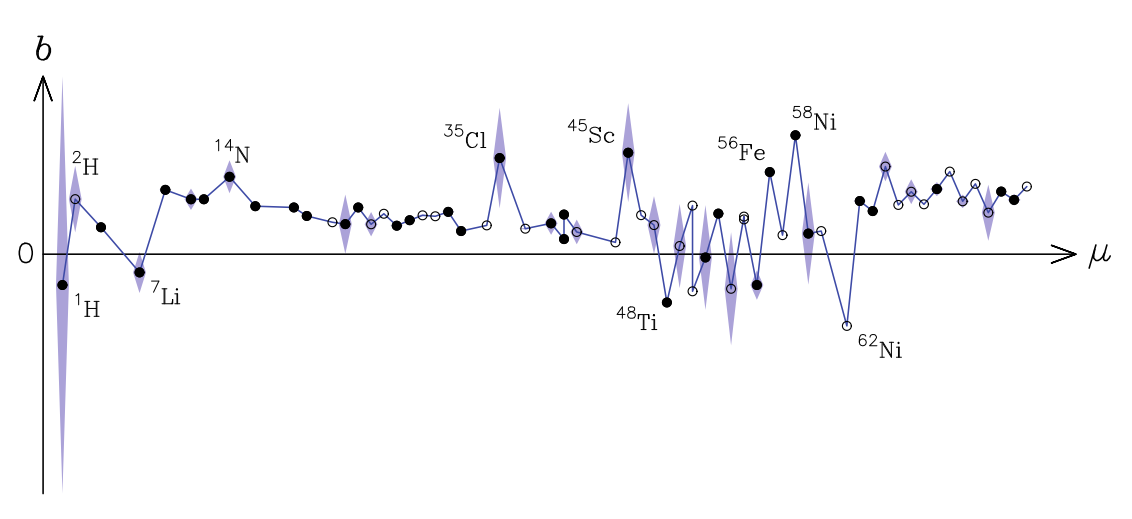
\includegraphics[width=0.85\textwidth]{theory/scatlen}
    \caption{The variation of the average neutron scattering length, $\langle b \rangle$ (circles), with atomic mass, $\mu$. The standard deviation, $\Delta b$, is indicated with the shaded regions. Reproduced, with permission of Oxford University Press\textsuperscript{\textcopyright}, from Reference~\cite{sivia_elementary_2011}.}
    \label{fig:scatlen}
\end{figure}
%
\begin{table}
    \centering
    \small
    \caption{Examples of coherent and incoherent scattering cross-sections, from Reference~\cite{schurtenberger_contrast_2002}.}
    \label{tab:crosssec}
    \begin{tabular}{r | c c c}
        \toprule
        Isotope & $S$ & $\sigma_{\text{coh}}$/\SI{e-28}{\meter\square} & $\sigma_{\text{incoh}}$/\SI{e-28}{\meter\square} \\
        \midrule
        \ce{^1H} & $\sfrac{1}{2}$ & 1.8 & 79.7 \\
        \ce{^2H} & 1 & 5.6 & 2.0 \\
        \ce{^{12}C} & 0 & 5.6 & -- \\
        \ce{^{14}N} & 1 & 11.6 & 0.3 \\
        \ce{^{16}O} & 0 & 4.2 & -- \\
        \bottomrule
    \end{tabular}
\end{table}
%

The difference between the scattering of \ce{^1H} and \ce{^2H}, evident in Table \ref{tab:crosssec}, can lead to a very useful technique in soft matter scattering, known as contrast variation.
The idea of contrast variation is based on the substitution of one isotope of an atom for another, while not introducing significant change to the properties of the material.
Traditionally the benefit of this came in terms of contrast matching out a part of the system to reduce the dimensionality of the problem for analysis.
For example, by matching the solvent scattering length density to that of the tails of the surfactants at the centre of a micelle there would only be scattered from the heads, and conversely, there would only be scattered from the tails if the solvent had the same scattering length density as the head groups.
This means that the problem becomes more straightforward as there are fewer variable parameters when fitting the data. This idea is represented graphically in Figure~\ref{fig:convar}.
%
\begin{figure}
    \centering
    
\includegraphics[width=0.85\textwidth]{theory/convar}
    \caption{The effect of varying the scattering length density of the solvent in a micelle system, (a) the system in a pure solvent, (b) the solvent is contrast matched to the surfactant tails, and (c) the solvent is contrast matched to the surfactant heads.}
    \label{fig:convar}
\end{figure}
%
The technique of contrast variation may also be used in terms of data analysis.
By increasing the number of data sets corresponding to a single model at different contrasts, the solution for the true structure of the model from the scattering data becomes more robust.
This is due to the fact that each different contrast can be considered as an independent measurement of the same system, and hence each set of scattering data can be used within the data analysis procedure to obtain the best global agreement to the experiment.
This co-refinement of multiple experiments can, under the right conditions, be used to simultaneously consider both neutron and X-ray datasets \cite{nelson_co-refinement_2006}.

There is also the possibility of using contrast variation when the probing radiation is the X-ray, through the use of anomalous scattering.
This is where different wavelengths of radiation give different scattering when the wavelengths are on opposite sides of an X-ray absorption edge.
This is not frequently used for soft matter species, as the X-ray absorption edges for elements common in soft matter (H, C, N, O, etc.) are at very low X-ray energies so generally outside of the accessible range of a standard SAXS instrument \cite{schurtenberger_contrast_2002}.

%\section{Classical simulation}
\label{sec:classical}

In order to simulate a real chemical system, it is necessary to model the electrons of the molecules and their interactions.
This is usually achieved using quantum mechanical calculations, where the energy of the system is calculated by finding some approximate solution to the Schr\"{o}dinger equation.
However, quantum mechanical calculations are very computationally expensive and are realistically limited to hundreds of atoms.
In order to simulate a soft matter system such as a lipid monolayer or polymer nanoparticles, it is necessary to simplify the calculation being performed.
This leads to classical simulation, where mathematical functions are used to determine the potential energy of the system.
Classical simulations are used substantially in this work, in terms of both molecular dynamics simulations and energy minimisation methods (see Section~\ref{sec:optimisation}).
Therefore, it is necessary to introduce the underlying theory on which this method is defined.

\subsection{Potential models}
\label{sec:potentmodels}
Potential modelling is a more computationally efficient method for the calculation of the potential energy of a chemical system.
A potential model consists of a series of mathematical functions that depend on the atomic positions, $\mathbf{r}$.
Each of the functions represents the potential energy of a different interaction for a given atom.
Broadly, these interactions can be split into bonded and non-bonded, such that the total energy may be described as follows,
%
\begin{equation}
  E_{\text{total}}(r) = E_{\text{bonded}}(r) + E_{\text{non-bonded}}(r)
\end{equation}
%
The total potential energy is then the sum of the potential energy for each of the individual atoms.

The bonded terms are used to describe different aspects of chemical bonds.
These typically consist of bond stretches, angle bends and dihedral torsions; within the OPLS2005 potential model \cite{banks_integrated_2005}, these interactions have the following mathematical form,
%
\begin{equation}
\begin{aligned}
  E_{\text{bonded}}(b, \theta, \phi) & = \sum_{\text{bonds}}K_b(b-b_0)^2 + \sum_{\text{angles}}K_{\theta}(\theta-\theta_0)^2 \\
  + \sum_{\text{dihedrals}} & \frac{1}{2}\big\{A_1[1 + \cos(\phi)] + A_2(1 - \cos(2\phi)] + A_3(1 + \cos(3\phi)]\big\},
\end{aligned}
\end{equation}
%
where, $K_b$ and $b_0$, $K_{\theta}$, $\theta_0$, and $A_1$, $A_2$, and $A_3$ are interaction dependent parameters for the bonds, angles, and dihedrals respectively, while $b$, $\theta$, and $\phi$ are the bond lengths, the size of the angles, and the size of the dihedrals that depend on the atom positions.
It can be seen that both the bond stretch and angle bend have harmonic functions, whereas the dihedral consists of a more complex multiple cosine functions.
The values of the interaction dependent parameters are determined as outlined in Section~\ref{sec:parameterisation}.

The non-bonded terms are a series of functions that describe the potential energy of intermolecular interactions, such as electrostatics and London dispersion forces.
The potential energies of the short-range interactions are usually modelled as a combination of the attractive London dispersion interaction and the repulsive exchange forces that arise from the Pauli exclusions principle \cite{leach_molecular_1996}.
These areoften forms such as shown below for the Lennard-Jones potential model \cite{lennard-jones_determination_1924},
%
\begin{equation}
  E_{\text{non-boned}}(r) = E_{\text{repulsive}} + E_{\text{attractive}} = \frac{A}{r^{12}} - \frac{B}{r^6} = 4\varepsilon\Bigg[\bigg(\frac{\sigma}{r}\bigg)^{12} - \bigg(\frac{\sigma}{r}\bigg)^6\Bigg]
\end{equation}
%
where, $r$ is the distance between two particles, $A$ and $B$ are interaction dependent parameters, and $\sigma$ and $\epsilon$ are simple reformations of these parameters,
%
\begin{equation}
  A = 4\varepsilon\sigma^{12} \;\;\;\; B = 4\varepsilon\sigma^6.
\end{equation}
%
Figure~\ref{fig:lj} shows each component of the Lennard-Jones potential model for atoms of argon, using parameters for $A$ and $B$ determined by Rahman \cite{rahman_correlations_1964}.
The Lennard-Jones is not the only potential model that may be used for the modelling of the short-range non-bonded interactions, others such as the Buckingham and Morse potentials exist \cite{buckingham_classical_1938, morse_diatomic_1929}.
However, the Lennard-Jones model has been used heavily in this work.
%
\begin{figure}
    \centering
    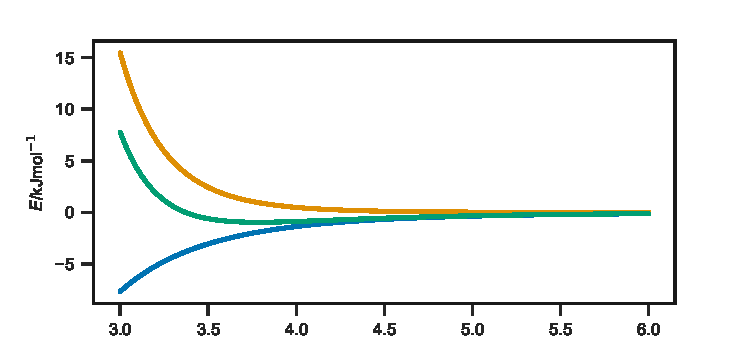
\includegraphics[width=0.85\textwidth]{theory/lj}
    \caption{The form of each component; attractive (blue), repulsive (orange), of the Lennard-Jones potential model (green) for argon, using parameters from Rahman \cite{rahman_correlations_1964}.}
    \label{fig:lj}
\end{figure}
%

While the short-range interactions are accounted for by a function such as the Lennard-Jones potential model, the potential energy of the long-range electrostatic interactions are usually modelled, more consistently, using Coulomb's law for classical electrostatic interaction between point particles \cite{coulomb_premier_1788, coulomb_second_1788},
%
\begin{equation}
  E_{\text{Coulomb}}(r) = \frac{1}{4\pi\varepsilon_0}{\frac{q_iq_je^2}{r^2}},
\end{equation}
%
where, $r$ is the distance between the two particles, $\varepsilon_0$ is the dielectric permittivity of the vacuum, $e$ is the charge of the electron, and $q_i$ and $q_j$ are the electronic charges on each of the particles.
It is clear that when $q_i$ and $q_j$ have the opposite signs Coulomb's law is always attractive.

An example of a very large classical simulation would be $\sim3$ million atoms \cite{gumbart_regulation_2009}.
However, this is still only \SI{1.8e-16}{\mol} which is not remotely realistic as a simulation of a \emph{real} system.
A common method to allow for the apparent simulation of a much larger system is the use of periodic boundary conditions.
This is where a boundary condition is applied to the edges of the simulation cell, such as to mimic an infinite system, assuming that the simulation cell is surrounded by identical images of itself (Figure~\ref{fig:pbc}).
Using the periodic boundary condition means that atomic diffusion is conserved as when an atom reaches the edge of the simulation cell, it will appear on the other side such that it came from the adjacent periodic time.
The use of a periodic boundary condition is particularly powerful in the simulation of homogenous systems, such as liquids.
However, the periodicity may result in unexpected results for particular systems, as is discussed in Chapter \ref{reflectometry2}.
%
\begin{figure}
    \centering
    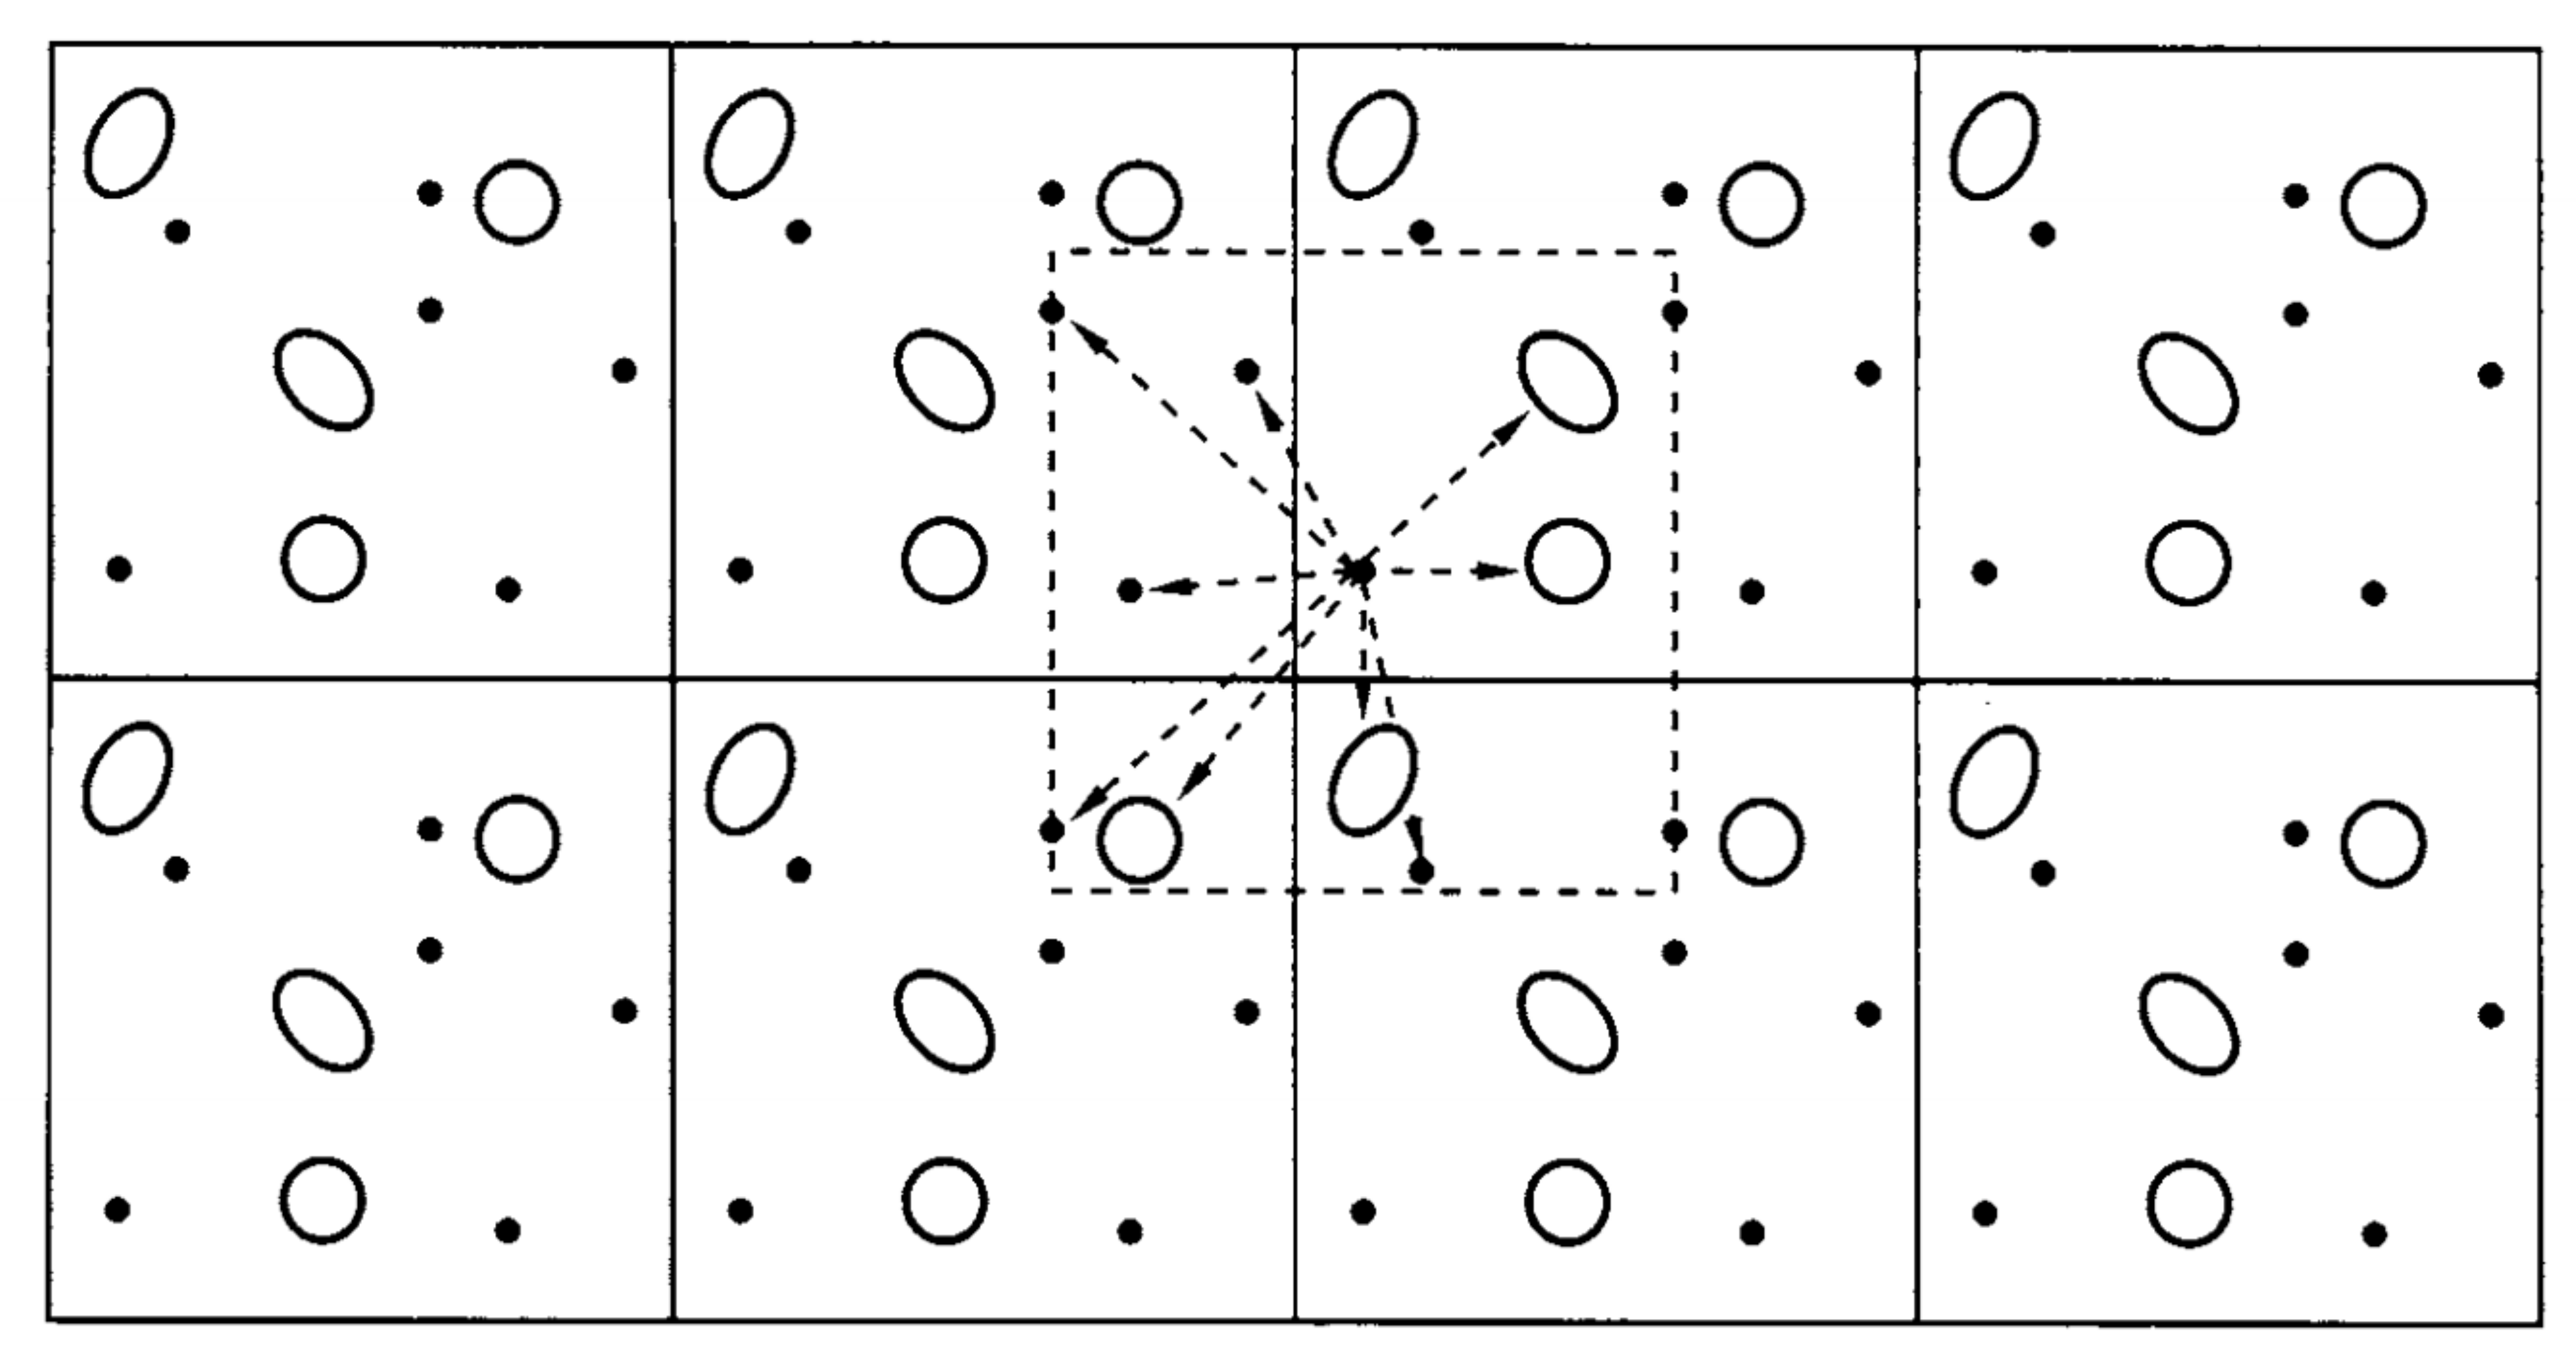
\includegraphics[width=0.85\textwidth]{theory/pbc}
    \caption{A graphical representation of the periodic boundary conditions. Reprinted by permission from Elsevier\textsuperscript{\textcopyright} from Reference~\cite{frenkel_understanding_1996}.}
    \label{fig:pbc}
\end{figure}
%

The periodic boundary condition leads to the necessity to consider another important factor from a classical simulation.
This is the cut-off, the distance after which the energy between to particles is considered to be zero.
The cut-off is an important component of simulation that must be considered as if there was no energy cut-off distance it would be possible for multiple counting of particle-particle interactions to occur.
This multiple counting would arise from counting between particles in different periodic images that have already been accounted for elsewhere.
As a result, the energy cut-off distance should always be less than half the shortest simulation cell vector.
An additional benefit of the energy cut-off distance is that means that it is not necessary to calculate the energy between every particle, as once the distance has been found to be greater than the cut-off distance the energy for this interaction is immediately taken as zero, increasing computational efficiency.
Code Block~\ref{cb:lj} gives an example of some code that could be used to calculate the Lennard-Jones energy of an atomistic system, where both the periodic boundary condition and the energy cut-off distance are considered.
%
\begin{figure}
    \centering
        \lstinputlisting[caption={Code that may be used to generate the Lennard-Jones energy for a given atomistic system, which accounts for the periodic boundary condition and the energy cut-off distance.},label={cb:lj}]{reports/code_blocks/lennardjones.py}
\end{figure}
%

The use of the periodic boundary condition may be problematic for systems containing long-range interactions, such as classical electrostatics.
Due to the fact that the range of the electrostatic interaction may be much greater than the size of half of the simulation cell, which is usually taken to be the energy cut-off distance.
In order to avoid truncation artefacts, the Ewald summation is often used for the calculation of the electrostatic contribution to the potential energy \cite{ewald_berechnung_1921}.
The Ewald summation involves performing the summation of the contributing interaction energies in reciprocal space rather than in real space as is the case for the short-range interactions.
Most modern molecular dynamics simulation software packages implement the Ewald summation using a particle mesh Ewald (PME) method \cite{essmann_smooth_1995}.

\subsection{Parameterisation}
\label{sec:parameterisation}
Section~\ref{sec:potentmodels} introduced the idea of potential models that may be used to evaluate the potential energy of a given system, much quicker than methods that rely on the use of quantum mechanics.
However, for these methods to be effective, it is important that the potential models used are able to model the system understudy accurately.
This is achieved initially by selecting the correct potential model for a given interaction, and then by ensuring that the interaction dependent parameters are accurate for a given interaction.
The method of obtaining such parameters is referred to as \emph{parameterising} the model.
Model parameterisation is important for all types of potential models, for example it is necessary to determine the equilibrium bond length $b_0$ and the force constant $K_b$ for a given covalent bonds, or the partial electrostatic charge that is present on a carbonyl oxygen atom when it interacts with the hydrogen atom from a neighbouring hydroxyl group.

Parameterisation of a potential model is usually achieved by comparison of fitting the potential model functions to energetic data obtained using a higher accuracy technique, such as quantum mechanical calculations or experimental methods.
We will not dwell on the details of potential model parameterisation, however, it is important to note that the parameters used on molecular dynamics simulation are not absolute and depended heavily on the merits of the parameterisation method.

In the work, we focused heavily on the use of off-the-shelf potential models.
The was done to ensure the easy reproducibility of the work.
Off-the-shelf potential models are those that are determined to be applied to a wide range of chemical systems, examples include the OPLS potential mode which was parameterised by comparison to quantum mechanical measurements and crystallographic data \cite{jorgensen_opls_1988}.
While these off-the-shelf potential models are useful for their ease-of-use, it is noted that often these forcefields may require to be optimised for the particular system.

\subsection{Coarse-graining}
\label{sec:coarsegraining}
The atomistic simulation of very large systems, such as multiple surfactant micelles or large lipid monolayers, require a huge number of atoms.
While computational efficiency improvements such as the periodic boundary condition or the energy cut-off distance are able to improve the time taken to simulate these systems.
However, it is still not possible to produce physically meaningful simulations without including some other efficiency improvements.

This has lead to the use of coarse-graining of molecules in simulations.
This is the definition of super-atoms, in the place of groups of atoms, known as `beading', some examples are shown for the MARTINI force field in Figure~\ref{fig:cg}.
Each of the super-atoms must correspond to the chemistry of the underlying atoms.
For example in the MARTINI potential model, there are five different carbon-like super-atoms that may be used dependent on the polarity of the carbon atoms that make up the super-atom.
%
\begin{figure}
    \centering
    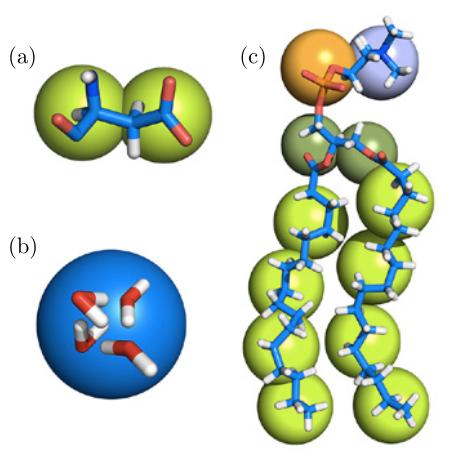
\includegraphics[width=0.85\textwidth]{theory/beading}
    \caption{Three examples of the MARTINI coarse-graining mechanism for (a) aspertic acid, (b) a water cluster, and (c) a molecule of DPPC, from Reference~\cite{pluhackova_biomembranes_2015}.}
    \label{fig:cg}
\end{figure}
%

In addition to the computational benefit of having fewer particles in the simulation, and therefore the equations of motion must be integrated fewer times.
There is also the opportunity to increase the timestep length for the simulation \cite{pluhackova_biomembranes_2015}.
This can be achieved as the highest frequency vibrations that must be modelled in the system are integrated out.
For example, the use of a united atom potential model, where the hydrogen atoms have been integrated out, the time step may be larger than for the same all-atom system as it is no longer necessary to model the high-frequency \ce{C-H} bond.

The technique of coarse-graining a molecule is a continuum, it can range from the integration of the hydrogen atoms into the heavier atoms to which they are bound, all the way to the treatment of entire molecules as a single `bead', with the inclusion of an implicit solvent.
The parameterisation of a coarse-grained potential model is carried out in much the same way as discussed in Section~\ref{sec:parameterisation} for all-atom potential models.
The coarse-grained parameters are determined by comparison with a higher-resolution technique, often this is all-atom molecular dynamics simulations.

%\section{Optimisation \& sampling methods}
\label{sec:optimisation}
In this work, computational modelling methods have been applied to important scattering problems.
The aim of many modelling problems is to optimise a series of parameters such that a minimum is found in some parameter-dependent metric.
While, in other circumstances, the aim is to sample the parametric search-space of a particular problem.
The problem of parameter optimisation and sampling is a massive area of mathematics and computer science and is it not possible to introduce the whole field.
Therefore, we will introduce two optimisation methods and two sampling methods that are applied within this work.

%\subsection{Single candidate optimisation methods}
%\label{sec:singlecan}
%Single candidate methods are optimisation procedures that operate in a linear fashion, where there is a single sample that must be optimised.
%These type of methods are often more straightforward than the population methods discussed later, however frequently they are only suitable for the determination of local minima.

%\subsubsection{Gradient descent}
%The gradient descent is a simple, analytic optimisation algorithm that is capable of determining the local minimum of a given function.
%This method involves determining the local gradient of the function, at a given position and using this to define how the position should be changed.
%For some arbitrary, multi-dimensional function, $F(\mathbf{p})$, where $\mathbf{p}$ is the position, this can be described as,
%
%\begin{equation}
%\mathbf{a} \leftarrow \mathbf{a} - \alpha \frac{\partial F(\mathbf{p})}{\partial \mathbf{a}},
%\end{equation}
%
%where $\alpha$ is a constant that defines the step-size and $\sfrac{\partial F(\mathbf{p})}{\partial \mathbf{p}}$ is the first derivative of the multi-dimensional function.
%It is necessary to find a suitable value for $\alpha$ for a given function.
%Therefore, the gradient descent method is often replaced with the more computationally expensive Newton-Raphson methods.
%The gradient descent method is shown applied to a Rosenbrock function \cite{rosenbrock_automatic_1960}, with a series of different step sizes in Figure~\ref{fig:grad}
%The gradient descent method is relatively simple to introduce, shown in Code Block~\ref{cb:grad}, however, it is only capable of finding local minima and therefore is often unsuitable for situations where the global minima are desired.
%
%\begin{figure}
%    \centering
%    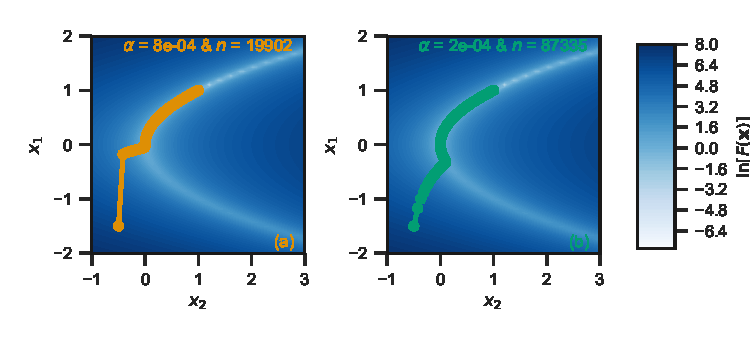
\includegraphics[width=0.85\textwidth]{theory/grad}
%    \caption{Example of the gradient descent method applied to a Rosenbrock function \cite{rosenbrock_automatic_1960}, where $a=1$ and $b=100$ (therefore the minima is at ($1$, $1$)), $n$ indicated the number of iterations required to minimise the values. Two different values (\SIlist{2e-4;8e-4}{}) for $\alpha$ are shown to emphasize the efficiency improvement that is possible with the optimisation.}
%    \label{fig:grad}
%\end{figure}
%
%
%\begin{figure}
%    \centering
%        \lstinputlisting[caption={An example of a simple implementation for the Gradient descent, as applied to a two-dimensional function.},label={cb:grad}]{reports/code_blocks/grad.py}
%\end{figure}
%

\subsection{Population optimisation methods}
Population-based algorithms make use of a population of candidate solutions.%, compared to the single candidate shown in the gradient descent method above.
This population of candidate solutions often have knowledge of the state of each other through some interaction method.
The method of interaction is often used to characterise the algorithms, into evolutionary algorithms (such as differential evolution), and swarm intelligence algorithms (such as the particle swarm method detailed below) \cite{wu_ensemble_2019}.
These population methods are usually more efficient at finding the global minimum for a given search space, than the single candidate methods described above.

\subsubsection{Differential evolution}
\label{sec:de}
Differential evolution (DE) is a common, iterative optimisation algorithm, that was first applied to the analysis of reflectometry and diffraction data by Wormington \emph{et al.} \cite{wormington_characterization_1999}.
Since then, it has proven very popular for the optimisation of reflectometry data and is included in many common analysis programs \cite{bjorck_fitting_2011,bjorck_genx_2007,nelson_co-refinement_2006,nelson_refnx_2019,ott_simulreflec_nodate,kienzle_ncnr_nodate}.
The DE algorithm is designed to more ably determine the global minimum of a particular function \cite{storn_differential_1997}.

DE is an example of a genetic algorithm, one that is designed to mimic the evolution processes observed in biology \cite{holland_adaptation_1992}.
The method consists of two vectors, the parent population, $\mathbf{p}$, the offspring population, $\mathbf{o}$.
These vectors are of a dimension $(i\times j)$, where $i$ is the number of variables being optimised and $j$ is the number of candidate solutions being used.
The offspring population vector is created through some trial methods, many of these exist however we will discuss a simple classical trial method, details of other methods may be found in the work of Bj\"{o}rck \cite{bjorck_fitting_2011}.

A classical trial method consists of two stages, mutation and recombination.
The mutation stage involves performing some mutation on the parent population to create a mutant vector, $\mathbf{m}$, analogous to the mutation in biologically evolutionary theory.
The magnitude of the mutation is dependent on the mutation constant, $k_m$,
%
\begin{equation}
\mathbf{m}_{i,j}= b_{i} + k_m(\mathbf{p}_{i,R1} - \mathbf{p}_{i,R2}),
\end{equation}
%
where $b_{i}$ is the best candidate solution in the parent population, and $\mathbf{p}_{i,R1}$ and $\mathbf{p}_{i,R2}$ are randomly choosen members of the parent population.
The mutation constant can be considered as a control variable for the size of the search radius, with a large $k_m$ corresponding to a larger search radius.

The recombination step creates the offspring population vector by taking a sample from either the parent population or mutant vectors with some frequency, which depends on the recombination constant, $k_r$,
%
\begin{equation}
    \mathbf{o}_{i,j} =
  \begin{cases}
    \mathbf{m}_{i,j}, & \text{where}\ X < k_r \\
    \mathbf{p}_{i,j}, & \text{otherwise}
  \end{cases}
\end{equation}
%
where, $X\sim U[0, 1)$.
The recombination constant controls the progress of the algorithm as it impacts the frequency with which mutation is introduced into the offspring population vector.

The final stage is to compare the offspring and parent population vectors, in the selection stage to create the new parent population for the next iteration.
The selection stage comprises of using some figure of merit, $\zeta$, to choose between the subunit from the offspring or parent population vector.
In our example, that figure of merit may be the agreement between some experimental data and our model, or for the example in Figure~\ref{fig:diff_evo} it is the value of the Ackley function \cite{ackley_connectionist_1987}, which we are trying to minimise.
%
\begin{equation}
    \mathbf{p}_{*,j} \leftarrow
    \begin{cases}
        \mathbf{o}_{*,j}, & \text{where}\ \zeta_{\mathbf{o}_{*,j}} < \zeta_{\mathbf{p}_{*,j}} \\
        \mathbf{p}_{*,j}, & \text{otherwise}
    \end{cases}
\end{equation}
%
where, the $*$ notation indicates all objects in the given population, and $\zeta_{\mathbf{o}_{*,j}}$ and $\zeta_{\mathbf{p}_{*,j}}$ are the figures of merit for the offspring and population population candidate solutions respectively.
%
\begin{figure}
    \centering
    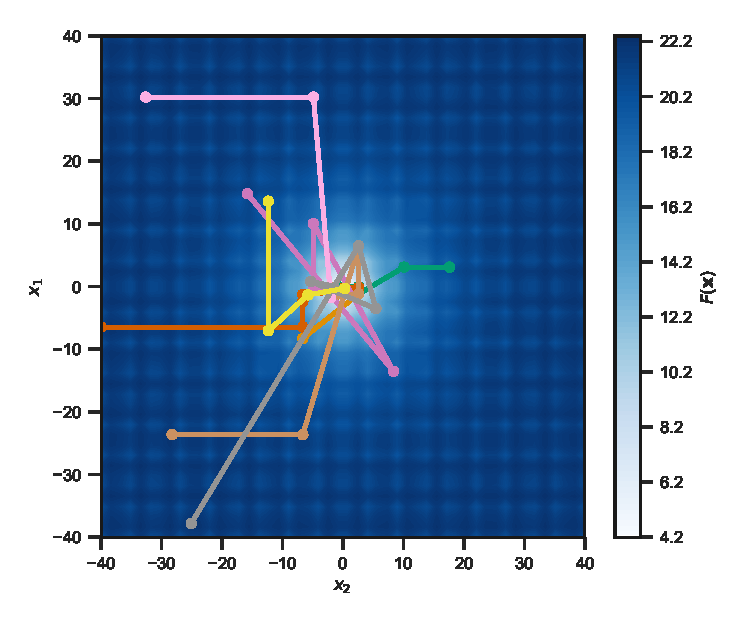
\includegraphics[width=0.85\textwidth]{theory/diff_evo}
    \caption{An example of a differential evolution (DE) algorithm as applied to an Ackley function \cite{ackley_connectionist_1987}, where $a=20$, $b=0.2$, and $c=2\pi$ (a common function for assessing global optimisation methods). The mutation and recombination constant in this implementation are both $0.5$. Each different coloured line represents a different candidate solution. The optimisation was stopped after $100$ iterations had run.}
    \label{fig:diff_evo}
\end{figure}
%

It is noted that it is often the case, in particular, when optimising experimental data, that there should be some bounds applied to the variables within the populations.
However, the DE algorithm may disregard these bounds due to the nature of the mutation step.
Therefore, it is common in DE algorithms, where bounds must be set, that if the search space moves outside that expected it is necessary to reinitialise the parameter.
An implementation of the DE algorithm is given programmatically in Code Block~\ref{cb:diff_evo}, where this reinitialisation is achieved by obtaining a new random number within the given bounds.
%
\begin{figure}
        \lstinputlisting[caption={An example of a simple implementation for a DE algorithm as described by Bj\"{o}rck \cite{bjorck_fitting_2011}.},label={cb:diff_evo}]{reports/code_blocks/diff_evo.py}
\end{figure}
%
%
\begin{figure}
    \centering
        \lstinputlisting[caption={The mutation step used in a classical trial method for a differential evolution algorithm, as described by Bj\"{o}rck \cite{bjorck_fitting_2011}.},label={cb:mut}]{reports/code_blocks/mutation.py}
\end{figure}
%
%
\begin{figure}
    \centering
        \lstinputlisting[caption={The recombination step used in a classical trial method for a differential evolution algorithm, as described by Bj\"{o}rck \cite{bjorck_fitting_2011}.},label={cb:recomb}]{reports/code_blocks/recombination.py}
\end{figure}
%
%
\begin{figure}
    \centering
        \lstinputlisting[caption={The selection step used in a differential evolution algorithm, as described by Bj\"{o}rck \cite{bjorck_fitting_2011}.},label={cb:sel}]{reports/code_blocks/selection.py}
\end{figure}
%

\subsubsection{Particle swarm}
\label{sec:partswarm}
Particle swarm optimisation (PSO) is a type of swarm intelligence population-based optimisation method.
This optimisation method was originally developed by Kennedy, Eberhart, and Shi for the simulation of social organisms such as bird flocks \cite{kennedy_particle_1995,shi_modified_1998}.
Particle swarm methods are particularly suitable for the optimisation, and sampling, of parametric search-spaces with a large number of similar minima, and therefore is useful for the study of the self-assembly of soft matter materials (Section~\ref{smallangle}).

These methods consist of a population vector, similar to that described for the differential evolution, that moves around the parametric search-space.
The motions of these `particles' are influenced by the positions of the other particles in the vector \cite{poli_analysis_2008}.
It is anticipated that this will lead the swarm to optimise the function under investigation.

Particles in the swarm are under the influence of two elastic forces.
The first attracts the particle to the best location in the search-space that the particle has found, while the other attracts the particle to the best search-space location found by any particle of the swarm.
The magnitudes of these forces are randomised but modulated by a pair of acceleration coefficients, $\psi_p$ that influences the attraction towards the personal best location, and $\psi_g$ that influences the attraction to the global best location.
The position of a particle changes between iterations of the algorithm based on the following relation,
%
\begin{equation}
\mathbf{p}_{*,j} \leftarrow \mathbf{p}_{*,j} + \mathbf{v}_{*,j},
\end{equation}
%
where, $\mathbf{p}_{*,j}$ is the position of the particle, and $\mathbf{v}_{*,j}$ is the velocity of the particle.
This velocity is determined as shown below,
%
\begin{equation}
\mathbf{v}_{*,j} \leftarrow \omega\mathbf{v}_{*,j} + \psi_gR1(\mathbf{g}_{*} - \mathbf{p}_{*,j}) + \psi_pR2(\mathbf{s}_{*,j} - \mathbf{p}_{*,j}),
\end{equation}
%
where, $\omega$ a constant known as the interia weight, $R1\sim U[0, 1)$ and $R2\sim U[0, 1)$ are random numbers, $\mathbf{g}_{*}$ is the best position occupied by any particle in the swarm and $\mathbf{s}_{*,j}$ is the person best for the particle $j$.

Figure~\ref{fig:part_swarm} shows an example of the particle swarm optimisation in action, applied to the Ackley function \cite{ackley_connectionist_1987}. Code Block~\ref{cb:part_swarm} shows a functional programmatic implementation of a particle swarm optimisation algorithm.
%
\begin{figure}
    \centering
    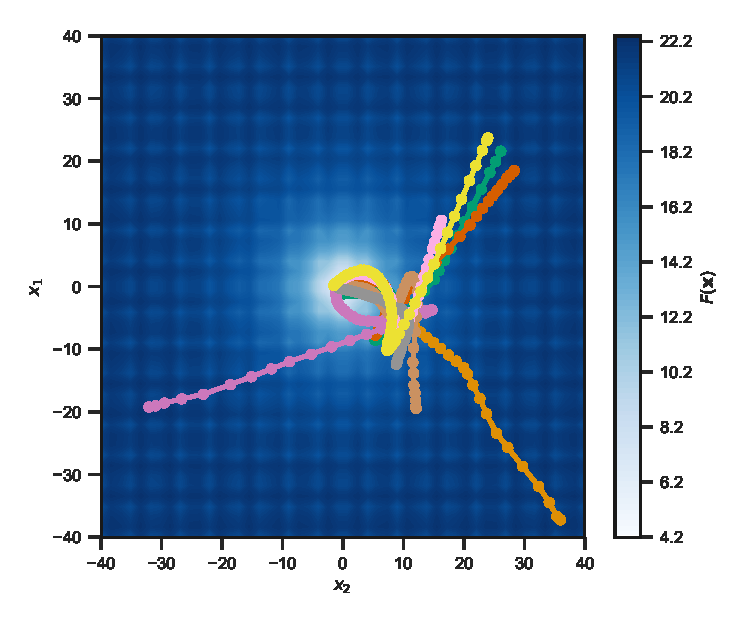
\includegraphics[width=0.85\textwidth]{theory/part_swarm}
    \caption{An example of a particle swarm optimisation as applied to an Ackley function \cite{ackley_connectionist_1987}, where $a=20$, $b=0.2$, and $c=2\pi$. For the particle swarm, the following parameters were used $\omega=0.9$, $\psi_g=0.05$, and $\psi_p=0.05$. Each different coloured line represents a different candidate solution. The optimisation was stopped after $100$ iterations had run.}
    \label{fig:part_swarm}
\end{figure}
%
\begin{figure}
    \centering
        \lstinputlisting[caption={An example of the particle swarm optimisation algorithm \cite{poli_analysis_2008}.},label={cb:part_swarm}]{reports/code_blocks/part_swarm.py}
\end{figure}
%

\subsection{Markov chain Monte-Carlo}
\label{sec:mcmc}
Markov chain Monte Carlo (MCMC) is a sampling methodology, derived from direct sampling Monte-Carlo \cite{krauth_statistical_2006}.
The aim of an MCMC algorithm is to sample a probability distribution, when parameters are described in terms of their degree of probability \cite{sivia_data_2006}.
Similar to molecular dynamics, in practical terms, MCMC should not be used on a system that is not already optimised, as its purpose is probability distribution sampling rather than minimisation.
Generally, the approach would be to optimise using, for example, one of the approaches described above, then to use MCMC or molecular dynamics to sample the appropriate search-space.
For example, in this work MCMC is used extensively, following the optimisation of a reflectometry model using a differential evolution algorithm, to quantify the inverse uncertainties of the model (this is the name given to the uncertainties in the parameters fitted in the modelling process).
In this context, the inverse uncertainty is the uncertainty on a given parameter within the model.
In addition to being able to give information about the inverse uncertainties, MCMC also offers a more complete understanding of the correlations present between the different parameters \cite{gilks_markov_1995}, as the interactions between the parameter variation has been quantified.

The aim of MCMC is to only sample configurations of a given function that are within the experimental uncertainty.
Figure~\ref{fig:mcmc} shows an example of the possible output that may be obtained from the application of an MCMC sampling method.
This was generated using a Metropolis-Hastings algorithm \cite{metropolis_equation_1953,hastings_monte_1970}, shown in Code Block~\ref{cb:mcmc}.
Initially, a Levenberg–Marquardt algorithm \cite{levenberg_method_1944,marquardt_algorithm_1963} was used to optimise the positions and integral of the two Gaussian functions that make up the data.
The MCMC was used to sample the values that were within the experimental uncertainty.
%
\begin{figure}
    \centering
    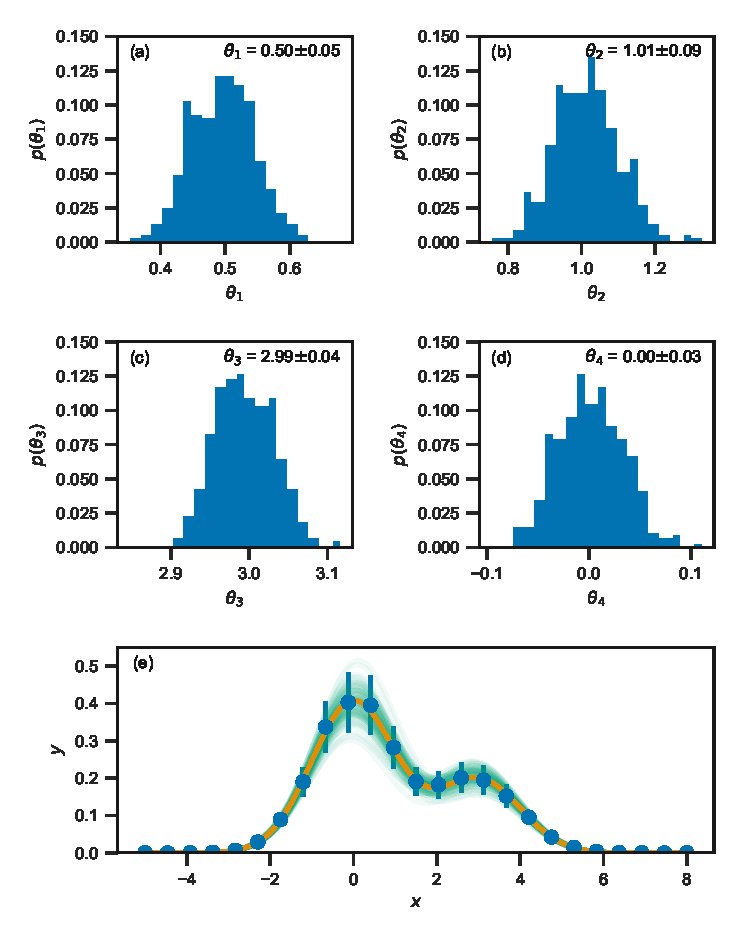
\includegraphics[width=0.85\textwidth]{theory/mcmc}
    \caption{An example of a four variable (two nearby Gaussian functions of different sizes with added random noise and some fractional uncertainty) problem probed using a MCMC method, using values of $a=0.1$, $\theta_1$ and $\theta_2$ correspond to the integral of the Gaussian function, while $\theta_3$ and $\theta_4$ indicate their positions; (a)-(d) histograms of the probability distribution function for each of the varibles, and (e) the data (blue circles), the optimised solution (orange line), and a series of probable solutions (green lines) showing the variability present in the data uncertainty.}
    \label{fig:mcmc}
\end{figure}
%
\begin{figure}
    \centering
        \lstinputlisting[caption={An example of the Metropolis-Hastings MCMC algorithm \cite{metropolis_equation_1953,hastings_monte_1970}.},label={cb:mcmc}]{reports/code_blocks/mcmc.py}
\end{figure}
%

Once an optimised solution, $\theta$, is obtained, the figure of metric is calculated, in Code Block~\ref{cb:mcmc} this is the agreement between the model and the experimental data, $\chi^2$, where,
%
\begin{equation}
\chi^2 = \sum\frac{(y_{\text{exp}} - y_{\text{calc}})^2}{\text{d}y_{\text{exp}}},
\end{equation}
%
and $y_{\text{exp}}$ is the experimental data, and $\text{d}y_{\text{exp}}$ the uncertainty in the experimental data, while $y_{\text{calc}}$ is the model solution.
Some random pertubation is then applied to the optimised solution,
%
\begin{equation}
\Theta = \theta + aR,
\end{equation}
%
where $R\sim N(0, 1)$ and $a$ is the step size.
A new $\chi^2$ is found for $\Theta$, and the probablity that this transition will occur is found,
%
\begin{equation}
p = \exp{\bigg(\frac{-\chi^2(\Theta) + \chi^2(\theta)}{2}\bigg)}.
\end{equation}
%
This probability is then compared with a random number $n\sim U[0, 1)$, and if $n$ is less than the probability, the new solution is stored,
%
\begin{equation}
\theta \leftarrow \Theta.
\end{equation}
%
This process is repeated until some desired number of samples has been obtained.
It should be noted that in the event on a poorly optimised initial value of $\theta$, it may be necessary to `burn' (that is to ignore) the first series of solutions while the MCMC algorithm settles into the search-space.

\subsection{Molecular dynamics}
\label{sec:md}
Section \ref{sec:classical} introduced classical potential models as a method for the evalution of the interaction energy of a given chemical system.
Any of the optimisation methods discussed above could be used alongside these classical potential models to find an energy minimum structure for the system or to sample the potential energy landscape.
However, it is often the case that we are interested in a dynamically relevant structure at a given temperature for some system.
This is where molecular dynamics simulations are a useful and important tool.

\subsubsection{Forces and accelertions}
The aim of a molecular dynamics simulation is to probe the positions, velocities, and accelerations on each of the atoms, or coarse-grained particles, as a simulation progresses.
The acceleration on a given particle, $\mathbf{a}$ is defined by the force on that particle, $\mathbf{f}$, in agreement with Newton's second law of motion,
%
\begin{equation}
\mathbf{f} = m\mathbf{a},
\label{equ:forcevec}
\end{equation}
%
where, $m$ is the mass of the particle.
In order to determine the acceleration on the particle, it is necessary to know the force on that particle.
The force, $f$, is a function of the potential energy, $E$, as found from a classical potential, of that atom,
%
\begin{equation}
f(r) = \frac{-\delta E_{\text{total}}(r)}{\delta r},
\label{equ:forcesca}
\end{equation}
%
where, $r$ is the configuration of the atoms.
Which is to say that, the force is the negative of the first derivative of the energy with respect to the atomic configuration.
The force found from Equation~\ref{equ:forcesca} is a scalar, however, we are interested in the force vector in Equation~\ref{equ:forcevec}.
To determine the force in a given direction, it is necessary to find the product of the force, $f$, and the unit vector in that direction,
%
\begin{equation}
\mathbf{f}_x = f\hat{\mathbf{r}}_x, \;\;\;\text{where}\;\hat{\mathbf{r}}_x = \frac{r_x}{|\mathbf{r}|},
\end{equation}
%
where $r_x$ is the atomic configuration in the $x$-dimension, and $|\mathbf{r}|$ is the magnitude of the atomic configuration vector.

\subsubsection{Integration}
The potential model, which we define for a given system, allows for the calculation of the acceleration on each particle in that system.
The next step is to use this acceleration to iterate through the trajectory of our system.
This is achieved by applying Newtonian equations of motion, for example in the Velocity-Verlet algorithm \cite{swope_computer_1982}.
%
\begin{equation}
\mathbf{x}(t + \Delta t) = \mathbf{x}(t) + \mathbf{v}(t)\Delta t + \frac{1}{2}\mathbf{a}(t)\Delta t^2, \\
\label{equ:vv1}
\end{equation}
\begin{equation}
\mathbf{v}(t + \Delta t) = \mathbf{v}(t) + \frac{1}{2}\big[\mathbf{a}(t) + \mathbf{a}(t+\Delta t)\big]\Delta t,
\label{equ:vv2}
\end{equation}
%
where, $\mathbf{x}$ is the position the particle $\mathbf{v}$ is the particle's velocity, and $\mathbf{a}$ is the particle's acceleration, while $t$ is current simulation time and $\Delta t$ is the timestep.
These equations constitute the Velocity-Verlet algorithm,
%
\begin{enumerate}
\item calculate the force (and therefore the acceleration) on each particle (Equations~\ref{equ:forcevec} \& \ref{equ:forcesca}),
\item find the position of the particle after some timestep (Equation~\ref{equ:vv1}),
\item determine the new velocity for each particle, based on the average acceleration at the current and new positions (Equation~\ref{equ:vv2}),
\item overwrite the old acceleration values with the new ones,
\item go to 1.
\end{enumerate}
%
Following an equilibration period, this algorithm may be iterated as many times as is required to obtain sufficient statistics for the measurement quantity of interest, e.g. particle positions for structural techniques such as elastic scattering.

The above analytical process is known as the integration step, and the Velocity-Verlet is the integrator.
If the size of the timestep $\Delta t$ is too large, the step size for a given iteration will not be accurate, as the forces on the atoms will change too significantly during it.
Therefore, the values of the timestep is usually on the order of \SI{10e-15}{\second} (\si{\femto\second}).
This means that in order to simulate a single nanosecond of ``real-time'' molecular dynamics, the integrator must be solved one million times.
This can be slow for very large systems, leading to an interest in coarse-grained simulations that result in fewer particles to determine the forces for (speeding up the integration step), but also enable to use of larger timesteps (so fewer integrations must be solved) \cite{rudd_coarse-grained_1998,brini_systematic_2013}, for example, the use of a MARTINI potential model allows for an upto twenty times increase in the timestep compared to an all-atom model.

\subsubsection{Initialisation}
The above discussion ignored two aspects that are necessary to run a molecular dynamics simulation, both of which as associated with the original configuration of the system; the original particle positions and velocities.

The particle positions are usually taken from some library, for example for the simulation of a protein, often the protein data bank \cite{noauthor_rcsb_nodate} is a useful resource.
Small molecules may be configured by hand using graphical programs such as Jmol \cite{noauthor_jmol_nodate}.
These small molecules may be built into complex, multicomponent structures using software such as the Packmol package \cite{martinez_packmol_2009}.
The importance of this initial structure cannot be overstated, for example, if the initial structure in a molecular dynamics simulation is unrepresentative of the equilibrium structure, it may take a large amount of simulation time before the equilibrium structure is obtained, possibly much longer than could be reasonably simulated.

The initial particle velocities are obtained in a much more general fashion.
They are selected randomly, and then scaled such that the kinetic energy, $E_k$, of the system agrees with a defined temperature, $T$,
%
\begin{equation}
E_k = \sum_{i=1}^N{\frac{m_i|\mathbf{v}_i|^2}{2}} = \frac{3}{2}Nk_BT,
\label{equ:ek}
\end{equation}
%
where, $m_i$ and $\mathbf{v}_i$ are the masses and velocities of the particles, $N$ is the number of particles, and $k_B$ is the Boltzmann constant.

\subsubsection{Ensembles}
The above algorithm details a simulation that makes use of an NVE ensemble, a simulation where the number of particles (N), the volume of the system (V), the energy of the system (E) are all kept constant.
However, this is not the only simulation ensemble that is available, within this work two other ensembles have been used extensively,
%
\begin{itemize}
\item the NVT (canonical) ensemble; this is similar to the NVE ensemble except the simulation temperature is controlled via a thermostat,
\item the NPT (isothermal-isobaric); this ensemble is similar to the NVT ensemble, however, the system volume is allowed to vary while the overall system pressure is held constant using a barostat.
\end{itemize}
%
Thermostating involves controlling the kinetic energy of the particles (Equation~\ref{equ:ek}) such that the simulation temperature is kept at a predefined value.
There are a variety of methods for thermostating a molecular dynamics simulation, such as the Andersen, Nos\'{e}-Hoover, or Berendsen methods \cite{andersen_molecular_1980,nose_unified_1984,berendsen_molecular_1984,hoover_canonical_1985}.
However, the most straightforward to describe, and that implemented in the \texttt{pylj} software (discussed in detail in Chapter \ref{teaching}) \cite{mccluskey_pylj_2018,mccluskey_arm61/pylj_2018} is a velocity rescaling \cite{bussi_canonical_2007}.
This is where the velocities for a random subset of the particles, $\mathbf{v}_i$ are adapted based on the following relation,
%
\begin{equation}
\mathbf{v}_i \leftarrow \mathbf{v}_i \sqrt{\frac{T_{\text{target}}}{\bar{T}}}
\end{equation}
%
where, $T_{\text{target}}$ is the target temperature, and $\bar{T}$ is the average simulation temperature.

The use of a barostat to control the simulation pressure usually involves varying the simulation cell parameters and the distances between the particles.
This would in a similar way to thermostating, where the simulation dimensions are scaled by a value in an effort to control the pressure.
The barostating methods are similar to the thermostating methods with Andersen, Nos\'{e}-Hoover, and Berendsen methods.
However, there is also the Parrinello-Rahman barostat which allows for independent control of the different cell dimensions giving control of stress in addition to pressure \cite{parrinello_polymorphic_1981}.

These optimisation and sampling methods were used in a variety of different applications within this work, firstly differential evoluation optimisation and MCMC sampling are used in Chapter~\ref{reflectometry1} in the study of a chemically-consistent modelling approach to X-ray and neutron reflectometry analysis.
Molecular dynamics simulation are investigated as a possible tool to assist in the analysis of reflectometry in in Chapter~\ref{reflectometry2}.
Finally, the particle swarm optimisation is applied for the efficient determination of a micelle structure for ftting small angle scattering data in Chapter~\ref{smallangle}.


% Chapter Template

\chapter{Chemically consistent modelling of X-ray and neutron reflectometry} % Main chapter title

\label{reflectometry1} % Change X to a consecutive number; for referencing this chapter elsewhere, use \ref{ChapterX}

%----------------------------------------------------------------------------------------
%	SECTION 1
%----------------------------------------------------------------------------------------

\section*{Abstract}
The work discussed in this chapter is the first example of the use of a chemically-consistent reflectometry model to co-refine X-ray reflectometry measurements at different surface pressures.
This was coupled with a differential evolution optimisation and Markov chain Monte Carlo sampling methodology in order to rationalise the parameter inverse uncertainties and correlations.
The chemically-consistent modelling approach was applied to the study of phospholipid monolayers at the air-deep eutectic solvent interface, which required that the head and tail group volume were not constrained.
By co-refining multiple experimental datasets, it was possible to accurately model the experimental data without these constraints present.

\section*{Context}
This project offers a severe method of coarse-graining for the analysis of neutron reflectometry\footnote{NR.} and XRR data.
The system is coarse-grained to represent a head group and a tail group of a phospholipid species.
There is a chemical constraint present in the model, such that the number of head groups must be equal to the number of pairs of tail groups.
However, there is no potential model considered beyond this ``bonded'' interaction.
Additionally, this modelling approach is applied again in Chapter~\ref{reflectometry2}, as an example of the cutting edge of traditional modelling, against which the classical simulation-driven methods are compared.
The specific application of this modelling approach grew from a collaboration with experimental colleagues working on self-assembly in DES.
Therefore, this chemical system will be briefly introduced in Section~\ref{sec:ref1intro}.
However, the main focus of this chapter will be the modelling methodology.

\pagebreak
\section{Introduction}
\label{sec:ref1intro}
\subsection{Deep eutectic solvents}
Deep eutectic solvents (DES) are a class of green, sustainable liquids that may be obtained from the combination of ionic species with compounds capable of acting as hydrogen bond donors, such as sugar, alcohols, amines, and carboxylic acids \cite{smith_deep_2014,dai_natural_2013}.
The resulting extensive hydrogen bonding network is capable of stabilising both species such that the eutectic mixture will remain liquid at room temperature \cite{hammond_liquid_2016,hammond_resilience_2017,araujo_inelastic_2017}.
Using different precursor materials can allow for the ability to tune the resulting solvent's physicochemical properties, such as polarity \cite{pandey_how_2014}, viscosity and surface tension \cite{smith_deep_2014}, network charge \cite{zahn_charge_2016}, and hydrophobicity \cite{ribeiro_menthol-based_2015,van_osch_hydrophobic_2015}.
Recently DES have also been shown to exhibit a ``solvophobic'' effect through the promotion of surfactant micelle formation \cite{sanchez-fernandez_micellization_2016,arnold_surfactant_2015,hsieh_micelle_2018,banjare_self-assembly_2018}, phospholipid bilayer formation \cite{bryant_spontaneous_2016,bryant_effect_2017,gutierrez_freeze-drying_2009}, and the ability to stability non-ionic polymer \cite{sapir_properties_2016} and protein conformations \cite{sanchez-fernandez_protein_2017}.

Phospholipid monolayers at the air/water interface have been widely studied as simplistic models for biological membranes.
As such, they have been used to gain insight into many biological processes that are technologically and medically relevant.
For example, investigations at the air/salt-water interface have identified the importance that interactions between charged phospholipid head groups and ions present in solution have on the structure, monolayer packing and stability \cite{mohwald_phospholipid_1990,kewalramani_effects_2010}.
However, the native environment for lipids in-vivo is far from simple aqueous solutions.
In fact, it has been suggested \cite{dai_natural_2013,hammond_resilience_2017} that DES might form within the crowded cellular environment and could assist in solubilizing biological species in an intermediate environment between that of the hydrophobic phospholipid tail groups and the highly polar water-rich regions, thereby assisting survival under extreme conditions such as freezing temperatures and drought where the water content of the cells is restricted.

This chapter presents the first observation of phospholipid monolayer at an air-DES interface.
Furthermore, this is one of a few examples of a phospholipid monolayer at the interface between air and a non-aqueous solvent, with only formamide noted previously \cite{graner_phospholipidic_1995}.
Langmuir monol;ayers of non-phospholipidic surfactant molecules have also been noted at air-formamide and air-mercury interfaces \cite{weinbach_self-assembled_1993,magnussen_self-assembly_1996,kraack_structure_2002}.
In these works, the authors noted that the non-aqueous surface had an effect on the overall structure of the monolayer, but little was said about the underlying mechanism.

\subsection{Optimisation and sampling in reflectometry analysis}
The analysis of reflectometry data usually involves the use of some model-dependency.
Therefore it is necessary to optimise the difference between our model, and the experimental dataset.
Analytical methods, such as the gradient descent method (Section~\ref{sec:singlecan}) are not usually suitable for application to the optimisation of a reflectometry model, as these are only capable of optimisation to local minima, which would require accurate prior knowledge of the model structure \cite{lovell_analysis_1999}.
Despite the analytical nature of the Maximum entropy (MaxEnt) optimisation method, this showed some success in the optimisation of reflectometry models, due in part to the ability of this optimisation to produce of a large number of solutions \cite{geoghegan_experimental_1996,bucknall_neutron_1997}.
This approach is computationally intensive and therefore it is unusual to apply it instead of other more efficient methods.
Some aspects of the MaxEnt methods were replicated in the work of Sivia \emph{et al.}, which employed Bayesian probability theory to rationalise the model selection \cite{geoghegan_experimental_1996,sivia_introduction_1993,sivia_bayesian_1998,sivia_analysis_1991}.

The use of analytic methods became less favoured as more frequently stochastic methods were used, as these offer a more pragmatic solution to the local minima problem.
These are methods that utilise inherently random behaviour to determine a global minimum.
The groove tracking method of Zhou and Chen \cite{zhou_model-independent_1993,zhou_theoretical_1995}, was one of the first examples of a stochastic optimisation process applied to the analysis of reflectometry data.
This randomly varied the scattering length density (SLD) of the layers in the model using a Monte Carlo approach.
A similar approach used a simulated annealing approach, with a ``temperature'' factor that decreased as the number of iterations increases \cite{kunz_model-free_1993}, however, this approach is still subject to the local minima problem as the probability of move acceptance decreased over time.

Both these Monte Carlo based approaches and the analytic methods previously discussed make the same perturbations to the fitted parameters during processing.
However, this is the cause of the propensity to converge to a local minimum.
This lead to the application of genetic algorithm derived methods for the optimisation of reflectometry models, beginning with the works of de Haan and Drijkoningen \cite{de_haan_genetic_1994} and Dane \emph{et al.} \cite{dane_application_1998}, who first applied this method to reflectometry analysis.
These methods are designed to stochastically sample an entire given search-space, and therefore are more able to overcome the local minima issues and determine the vicinity of a global minimum.
Following this initial application, genetic algorithms were used frequently in the optimisation of reflectometry models \cite{ulyanenkov_genetic_2000,ulyanenkov_extended_2005,politsch_unbiased_2002,wormington_characterization_1999}.
In particular, the work of Wormington \emph{et al.} \cite{wormington_characterization_1999} showed the applicability of the differential evolution method towards reflectometry model optimisation, which resulted in the inclusion of such methods in many common reflectometry analysis software packages \cite{bjorck_fitting_2011,bjorck_genx_2007,nelson_co-refinement_2006,nelson_refnx_2019,ott_simulreflec_nodate,kienzle_ncnr_nodate}.

The use of Markov chain Monte Carlo (MCMC) methods to probe the probability distribution functions of the fitting parameters of a reflectometry model have grown in popularity \cite{gil_limitations_2012,hoogerheide_structure_2018,owejan_solid_2012,heinrich_myristoylation_2014}.
This is due to the inclusion of MCMC methods in common analysis software packages such as Refl1D \cite{kienzle_ncnr_nodate}.
These methods enable the user to better understand the inverse uncertainties for the model.
Additionally, they enable the quantification of the correlation between parameters, important in ensuring that the model applied is suitably constrained such as to reduce the cross-correlation present between parameters \cite{nelson_co-refinement_2006}.

This work applies a differential algorithm \cite{storn_differential_1997,jones_scipy_nodate} to the optimisation of the reflectometry model.
The search-space, available within the experimental uncertainty of the data is then sampled using MCMC, as implemented in \texttt{emcee} \cite{foreman-mackey_emcee_2013}, to understand the parameter probability distributions and quantify the inter-parameter correlations.

\subsection{Chemically-consistent modelling}
The use of chemically-consistent modelling is common in the fitting of X-ray and neutron reflectometry measurements from phospholipid monolayers to obtain structural insights.
The history of this modelling is introduced well by Campbell \emph{et al.} \cite{campbell_structure_2018}.
While it is possible to model the neutron reflectometry from a phospholipid monolayer with a single layer model \cite{wojciechowski_interaction_2016,wojciechowski_complexation_2016}, the use of at least two layers; representing the head and tail groups is more commonplace \cite{foglia_interaction_2014,bello_influence_2016}.
Even when two layers are utilised, it is often the case that the volumes of the head and tail groups, $V_i$, are used as constraints in the modelling process, as the scattering length density ($\text{SLD}$) of a layer may be determined as follows,
%
\begin{equation}
\text{SLD}_i = \frac{b_i}{V_i}(1-\phi_i)+\text{SLD}_s(\phi_s)
\label{equ:sld}
\end{equation}
%
where, $b_i$ is the scattering length of the head or tail, $\phi_i$ is the volume fraction of solvation by the solvent, $\text{SLD}_s$ is the solvent scattering length density, and $i$ indicates either the head or tail layer.
However, as noted by Campbell \emph{et al.} \cite{campbell_structure_2018}, this method often fails to account for the compaction of the carbon chains under elevated surface pressures \cite{mcconlogue_close_1997,small_lateral_1984}, which may lead to a volume reduction of up to \SI{\sim 15}{\percent}.
Furthermore, as discussed in Section~\ref{refl1:anal}, the use of a constrained head group volume may also influence the result of the modelling process in situations where the volume is poorly defined.

Equation~\ref{equ:sld} enables the use of chemical-inference in the modelling approach for reflectometry data.
This allows for the co-refinement of neutron reflectometry data where different isotopic-contrasts of the phospholipid species or solvent have been used.
This is possible based on the expectation that the effect of contrast variation on the structure and chemistry of the monolayer will be negligible, and therefore the same values of all parameters in the fitting, except $b_i$ and $\text{SLD}_s$ may be constrained between the different measurements \cite{hollinshead_effects_2009}.
In this work, similar logic was applied, with the assumption that the volume of the head and tail groups is constant across different surface pressures, while the lipid phase is the same.
This means that, for this system, all of the fitted parameters may be constrained aside from the tail thickness, head solvation, and interfacial roughness, across the different surface pressure measurements.
This is the first time that such a methodology has been applied to the analysis of XRR and NR, additionally, it is believed that this ability to co-refine XRR measurements enables a greater understanding of the structure than that possible from a single measurement.

\section{Experimental}
The experimental measurements were designed and conducted by Drs Tom Arnold, Andrew Jackson, Adrian Sanchez-Fernandez, and Prof. Karen Edler, with the assistance of Dr Richard Campbell.
My role in this work was entirely on the analysis of the measurements and the development of the chemically-consistent model.
However, it is necessary to briefly discuss the materials and experimental methods used to enable a complete understanding of the context of the work.

\subsection{Materials}
Choline chloride (\SI{99}{\percent}, Sigma-Aldrich), glycerol (\SI{99}{\percent}, Sigma-Aldrich), d$_{9}$-choline chloride (\SI{99}{\percent}, \SI{98}{\percent} D, CK Isotopes), and d$_{8}$-glycerol (\SI{99}{\percent}, \SI{98}{\percent} D, CK Isotopes) were used in the preparation of the deep eutectic solvent (DES).
This is achieved by mixing a $1$:$2$ ratio of choline-chloride and glycerol and heating at \SI{80}{\celsius} until a homogeneous, transparent liquid is formed \cite{smith_deep_2014}.
This was then stored under a dry atmosphere to reduce the amount of water dissolved in the solvent.

The limited availability of deuterated precursors lead to only a fully protonated (hDES) and a partially deuterated (hdDES) being prepared and used in the neutron reflectometry measurements.
The partially deuterated subphase was prepared using the following mixtures of precursors: \SI{1}{\mole} of \SI{0.38}{\mole} fraction of h-choline-chloride/\SI{0.62}{\mole} fraction of d-choline-chloride; and \SI{2}{\mole} of \SI{0.56}{\mole} fraction of h-glycerol/\SI{0.44}{\mole} fraction of d-glycerol.

The water content of the DES was assessed before and after each experiment by Karl-Fisher titration (Mettler Toledo DL32 Karl-Fischer Coulometer, Aqualine Electrolyte A, Aqualine Catholyte CG A) and found to be always below \SI{0.3}{wt/\percent}.
This was taken to be a negligible amount and would not have a considerable impact on the DES characteristics \cite{hammond_liquid_2016,hammond_resilience_2017}.

1,2-dipalmitoyl-\emph{sn}-glycero-3-phosphocholine (DPPC, C$_{16}$ tails, \SI{>99}{\percent}), 1,2-dimyristoyl-\emph{sn}-glycero-3-phosphocholine (DMPC, C$_{14}$ tails, \SI{>99}{\percent}), and the sodium salt of 1,2-dimyristoyl-\emph{sn}-glycero-3-phospho-(1'-rac-glycerol) (DMPG, C$_{14}$ tails, \SI{>99}{\percent}) were obtained from Avanti Polar Lipids and 2-dilauroyl-\emph{sn}-glycero-3-phosphocholine (DLPC, C$_{12}$ tails, \SI{>99}{\percent}) was obtained from Sigma Aldrich and all were used without further purification. Deuterated versions of DPPC (d$_{62}$-DPPC, \SI{>99}{\percent}, deuterated tails-only) and DMPC (d$_{54}$-DMPC, \SI{>99}{\percent}, deuterated tails-only) were obtained from Avanti Polar Lipids and used without further purification.
These lipids were dissolved in chloroform solution (\SI{0.5}{\milli\gram\per\milli\liter}) at room temperature.
PC indicates where the phospholipid molecule contains a phosphocholine head group, while PG indicates a phosphatidylglycerol head group, the chemical structures of these can be seen in Figure~\ref{fig:heads}.
%
\begin{figure}
    \centering
    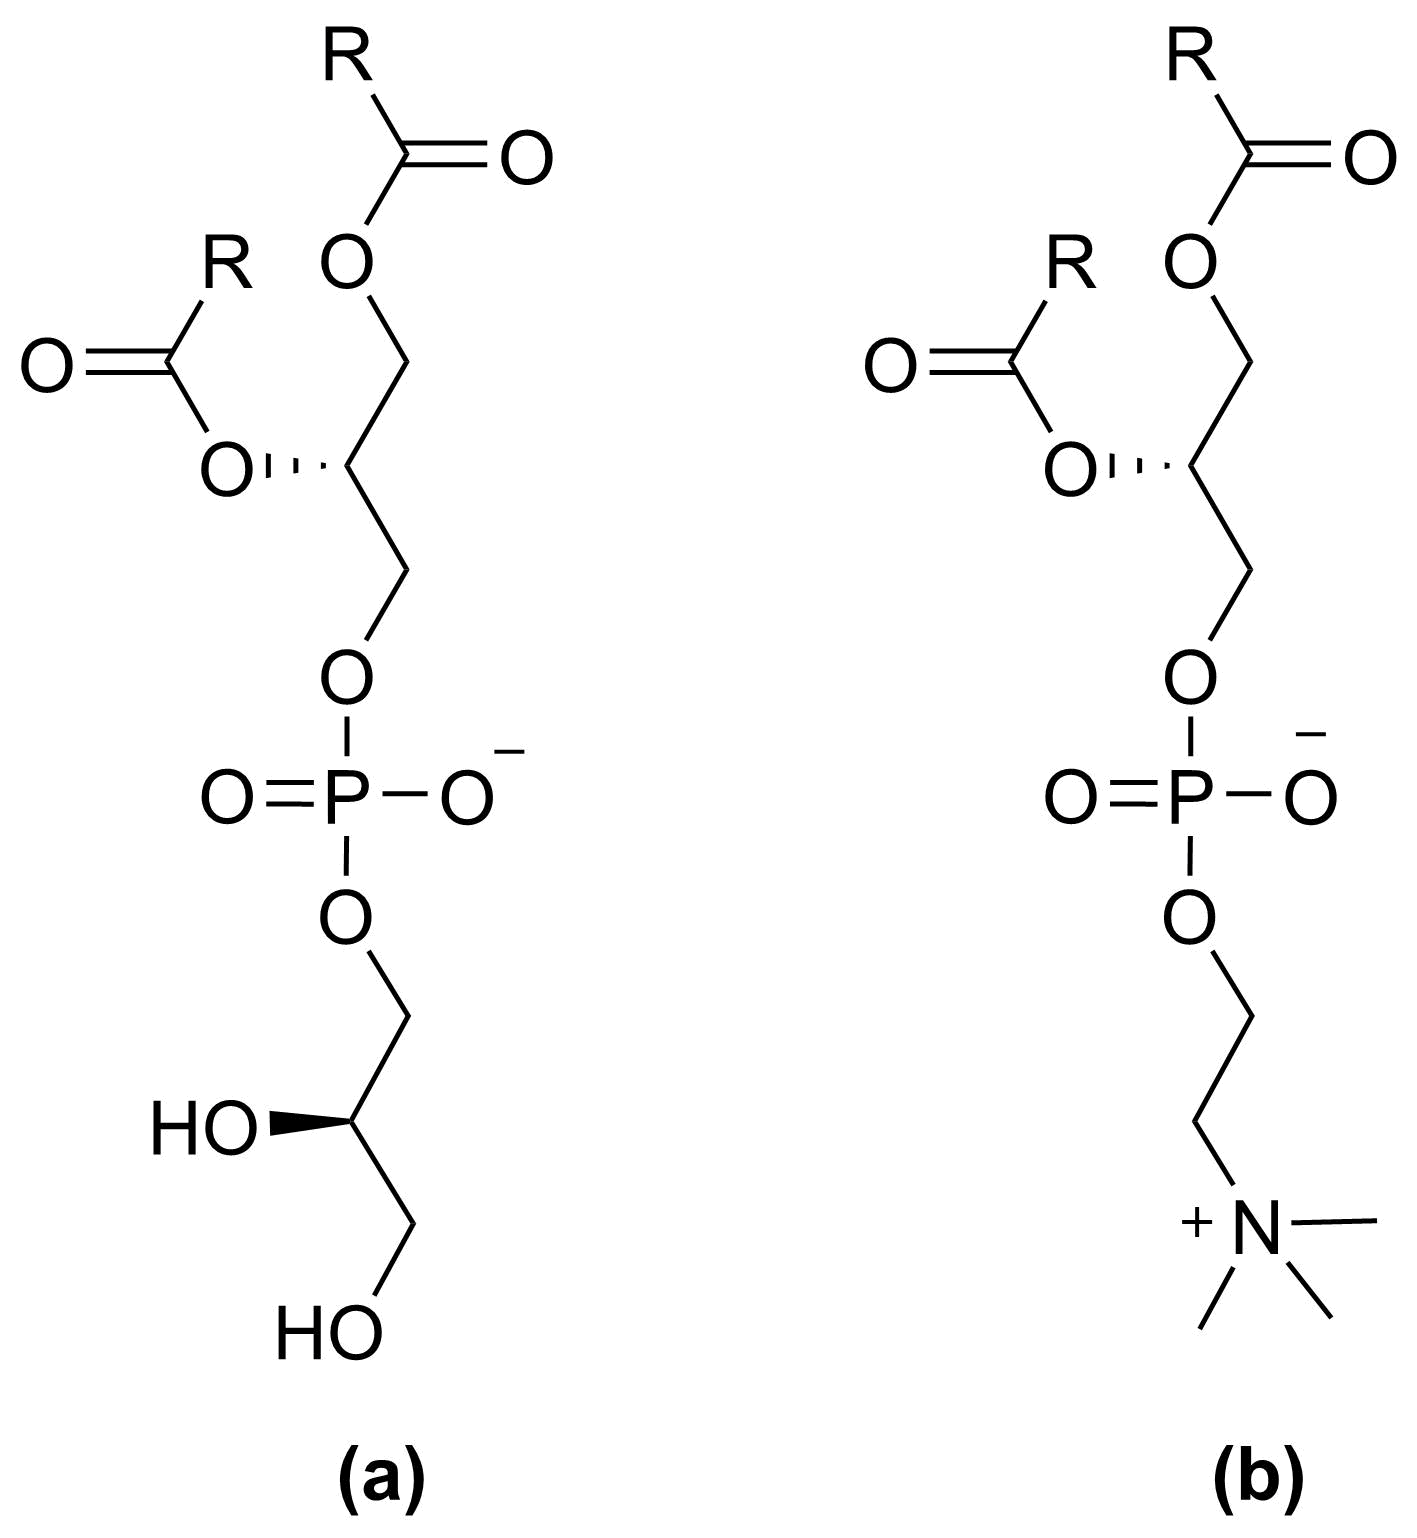
\includegraphics[width=0.40\textwidth]{reflectometry1/head_groups}
    \caption{The two phospholipid forms investgated in this work, where R indicates the hydorcarbon tail; (a) phosphatidylglycerol (PG), (b) phosphocholine (PC).}
    \label{fig:heads}
\end{figure}
%

In the X-ray reflectometry (XRR) experiment, the sample was prepared in-situ using the standard method for the spreading of insoluble monolayers on water: a certain amount of the phospholipid solution was spread on the liquid surface.
Following the evaporation of the chloroform, it is assumed that the resulting system is a subsurface of solvent with a monolayer of the phospholipid at the interface.
The surface concentration is then controlled by opening and closing the polytetrafluoroethylene (PFTE) barriers of a Langmuir trough.
To reduce the volumes used in the neutron reflectometry (NR) experiments, a small Delrin adsorption trough was used that did not have controllable barriers.
Therefore, although the surface concentration was nominally the same as for the XRR, the lack of precise control meant that it was determined to be inappropriate to co-refine the XRR and NR contrasts together.

\subsection{Methods}
The XRR measurements were carried out at the I07 beamline at the Diamond Light Source, with a photon energy of \SI{12.5}{\kilo\electronvolt} using the double-crystal deflector system \cite{arnold_implementation_2012}.
The reflected intensity was measured for a $q$ range of \SIrange{0.018}{0.7}{\per\angstrom}.
The data were normalised with respect to the incident beam and the background was measured from off-specular reflection and subsequently subtracted.
All of the samples were allowed at least one hour to equilibrate and preserved under an argon atmosphere.
XRR data were collected for each of the phospholipids, DLPC, DMPC, DPPC, and DMPG at four surface pressures each (DLPC: \SIlist{20;25;30;35}{\milli\newton\per\meter}, DMPC: \SIlist{20;25;30;40}{\milli\newton\per\meter}, DPPC: \SIlist{15;20;25;30}{\milli\newton\per\meter}, DMPG: \SIlist{15;20;25;30}{\milli\newton\per\meter}), as measured with an aluminium Wilhelmy plate; measurements were conducted at \SIlist{7;22}{\celsius}.
An aluminium Wilhelmy plate was used over a traditional paper due to the low wettability of paper by the DES.

The NR experiments were performed on the FIGARO instrument at the Institut Laue-Langevin using time-of-flight methods \cite{campbell_figaro_2011}.
Data were collected at two incident angles; \SIlist{0.62;3.8}{\degree}, providing a $q$ range from \SIrange{0.005}{0.18}{\per\angstrom}.
Two surface pressures for each phospholipid and contrast were measured (DMPC: \SIlist{20;25}{\milli\newton\per\meter}, DPPC: \SIlist{15;20}{\milli\newton\per\meter}).
As with the XRR measurements, the samples were given at least one hour to equilibrate, kept under an inert atmosphere.
All measurements were conducted at \SI{22}{\celsius}.

\section{Data analysis}
\label{refl1:anal}
XRR and NR methods have a well documented history for the analysis of the structure of phospholipid monolayers at the air-water interface \cite{mohwald_phospholipid_1990,kewalramani_effects_2010,bayerl_specular_1990,johnson_structure_1991,clifton_role_2012,helm_phospholipid_1987,daillant_x-ray_1990}.
Typically these have involved using a model-dependent analysis method, however, the modelling approaches have varied significantly in the number of layers used, the shape of the layers, the use of interfacial roughness, the parameterisation of constraints employed, and even the method by which the reflectometry profile was calculated from the model.
Recently, an evaluation of the applicability of different models for surfactant and phospholipid monolayers using NR outlined a view of ``best practice'' \cite{campbell_structure_2018}.
However, frequently the constraints employed in the modelling process include the head and tail volume for the phospholipid head and tail groups.
These values are taken from a variety of other techniques, some examples are shown in Table~\ref{tab:water}.
%
\begin{sidewaystable}
    \centering
  \small
    \caption{Lipid component volumes extracted from different literature sources. $V_l$ corresponds to the total phospholipid volume, $V_t$ to the tail group volume, $V_h$ to the head group volume, MD to molecular dynamics simulations, WAXS to wide-angle X-ray scattering, NB to neutral buoyancy, and DVTD to differential vibrating tube densimetry.}
    \label{tab:water}
    \begin{tabular}{l | l l l | l l | l l | l | l}
        \toprule
        Phospholipid & \multicolumn{3}{l|}{DPPC} & \multicolumn{2}{|l|}{DMPC} & \multicolumn{2}{|l|}{DLPC} & DMPG & POPG \\
        \midrule
    Ref. & \cite{armen_phospholipid_1998} & \cite{sun_order_1994} & \cite{kucerka_determination_2004,balgavy_evaluation_2001}\footnote{The values for the head component in Ku\v{c}erka \emph{et al.} \cite{kucerka_determination_2004}, were taken from Balgav\'{y} \emph{et al}. \cite{balgavy_evaluation_2001}} & \cite{armen_phospholipid_1998} & \cite{kucerka_determination_2004,balgavy_evaluation_2001} & \cite{armen_phospholipid_1998} & \cite{kucerka_determination_2004,balgavy_evaluation_2001} & \cite{pan_molecular_2012} & \cite{kucerka_scattering_2012} \\
    \midrule
    $V_l$/\si{\angstrom\cubed} & \num{1287.3 \pm 25.5} & \num{1148 \pm 2} & \num{1268.2 \pm 32.1} & \num{1172.5 \pm 25.1} & \num{1155.4 \pm 30.0} & \num{1057.7 \pm 24.7} & \num{1046.6 \pm 28.0} & \num{1011.4} & \num{1203} \\
    $V_t$/\si{\angstrom\cubed} & \num{966.4 \pm 5.4} & \num{829 \pm 4} & \num{924.7 \pm 17.6} & \num{851.5 \pm 5.0} & \num{815.9 \pm 15.5} & \num{736.8 \pm 4.6} & \num{707.1 \pm 13.5} & \num{720.4} & \num{914} \\
    $V_h$/\si{\angstrom\cubed} & \num{320.9 \pm 20.1} & \num{319 \pm 6} & \num{339.5 \pm 14.5} & \num{320.9 \pm 20.1} & \num{339.5 \pm 14.5} & \num{320.9 \pm 20.1} & \num{339.5 \pm 14.5} & \num{291.0} & \num{289} \\
    \midrule
    Method & MD & WAXS & NB & MD & NB & MD & NB & DVTD & MD \\
    T/\si{\celsius}& 50 & 24 & 30 & 50 & 30 & 50 & 30 & 20 & 25 \\
        \bottomrule
    \end{tabular}
\end{sidewaystable}
%

Table~\ref{tab:water} provides a general consensus that the volume of the phosphocholine head group (PC) is \SIrange{320}{360}{\angstrom\cubed}, while the phosphatidylglycerol head group (PG) is \SIrange{289}{291}{\angstrom\cubed}.
However, these values were all determined from experiments \cite{sun_order_1994,kucerka_determination_2004,balgavy_evaluation_2001,pan_molecular_2012} or simulations \cite{armen_phospholipid_1998,kucerka_scattering_2012} where the head group was interacting with water molecules.
It is not clear if this will influence the volume that it occupies, and if that volume will change in the presence of a non-aqueous solvent, such as the DES considered herein.
The charged nature of the zwitterionic and anionic phospholipid head groups may have different interactions with the polar, but neutral water and the charged DES \cite{sanchez-fernandez_self-assembly_2018}.
Additionally, it is known that, on water, increased surface pressures and the associated Liquid-Expanded to Liquid-Condensed phase transition will lead to a compression of the phospholipid tail volume, compared to the values in Table~\ref{tab:water} \cite{marsh_molecular_2010,small_lateral_1984}, and that this compaction has not necessarily been accounted for in the literature \cite{campbell_structure_2018}.

These factors meant that it was necessary to develop a model that was appropriate for the phospholipid chemistry while applying as much of the ``best practice'' from Campbell \emph{et al.} \cite{campbell_structure_2018} as possible, and ensuring that the head and tail group volumes were not constrained parameters.
The lack of having these normally constrained parameters meant that it was necessary to consider methods by which the reflectometry measurements could be co-refined, in a similar fashion to contrast variation co-refinement in neutron reflectometry.
This could be achieved by the co-refinement of reflectometry measurements at different surface pressures, as the model was appropriate for the phospholipid chemistry, and the different surface pressures were in the same phase; Liquid-Condensed (LC) for DPPC and Liquid-Expanded (LE) for DMPC, DLPC, and DMPG.
Therefore the head and tail group volumes will remain constant, and only the surface concentration and normal tail thickness will vary.

The chemically-constrained model that has been used in this work was implemented in the Python library \texttt{refnx} \cite{nelson_refnx_2019,nelson_refnx_2019-1}.
The software enables the inclusion of custom model classes that feed parameters into the Abel\`{e}s model (Section~\ref{sec:refltheory}) \cite{abeles_sur_1948,parratt_surface_1954}.
Our chemically-consistent model class can be seen in Code Block~\ref{cb:chemconsis}, and is shared under a CC BY-SA 4.0 license in the ESI for the associated publication \cite{mccluskey_lipids_at_airdes_2019}.
In order to ensure that the phospholipid chemistry was consistent both within the phospholipid molecule and across the different surface pressures, Code Block~\ref{cb:const} was implemented.
%
\begin{figure}
    \centering
        \lstinputlisting[caption={The chemically-consistent model class that was implemented in \texttt{refnx} \cite{nelson_refnx_2019,nelson_refnx_2019-1}.},label={cb:chemconsis},firstline=1,lastline=72]{reports/code_blocks/mol_vol.py}
\end{figure}
%
\begin{figure}
    \centering
        \lstinputlisting[caption={The \texttt{set\_constraints} that was used to impose chemical-consistency on the phospholipid monolayer structure..},label={cb:const},firstline=5,lastline=22]{reports/code_blocks/ref_help.py}
\end{figure}
%

The chemically-consistent model, that is outlined in Code Block~\ref{cb:chemconsis}, consisted of two layers that define the phospholipid monolayer; the head layer at the interface with the solvent and the tail layer at the air interface.
The head groups have a scattering length that can be calculated from a summation of the X-ray or neutron atomic scattering lengths, $b_h$, and a volume, $V_h$.
These groups make up a layer of a given thickness, $d_h$, which has some interfacial roughness, $\sigma_h$, within which some volume fraction of solvent may penetrate, $\phi_h$.
The tail layer is defined in the same way, however, the tail thickness, $d_t$, is constrained such that it can be no greater than the maximum extended length for the phospholipid tail (defined as the Tanford length, $t_t$ \cite{tanford_hydrophobic_1980}), which is given in Table~\ref{tab:invar}, and that no solvent may penetrate into the layer (e.g. $\phi_t=0$).
Therefore, the $\text{SLD}$ may be determined as discussed in Equation~\ref{equ:sld}.
Based on the work of Campbell \emph{et al.} \cite{campbell_structure_2018}, a single value for the interfacial roughness was fitted for all of the interfaces, including the subphase (i.e. $\sigma_t = \sigma_h = \sigma_s$), as there is only a single phospholipid molecule type present in each monolayer.
Therefore, any capillary wave roughness at the air-DES interface is carried monotonically through the layers. The interfacial roughness was constrained to be greater than \SI{3.3}{\angstrom}, in agreement with previous work \cite{sanchez-fernandez_micellization_2016}.
%
\begin{table}
    \centering
  \small
    \caption{The invarient parameters within the chemically-consistent model.}
    \label{tab:invar}
    \begin{tabular}{l | l l l | l}
        \toprule
        Component & $b_t$/\si{\femto\meter} & $b_h$/\si{\femto\meter} & $t_t$/\AA & $\text{SLD}$/$10^{-6}$ \AA$^{-2}$ \\
        \midrule
    X-ray & & & & \\
        DPPC & 6827 & 4635 & 20.5\tablefootnote{\label{note:tanford}Values obtained from the Tanford formula \cite{tanford_hydrophobic_1980}.} & -- \\
        DMPC & 5924 & 4635 & 18.0\footref{note:tanford} & -- \\
        DLPC & 5021 & 4635 & 15.5\footref{note:tanford} & -- \\
        DMPG & 5924 & 4694 & 18.0\footref{note:tanford} & -- \\
        Air & -- & -- & -- & 0 \\
        DES & -- & -- & -- & 10.8\tablefootnote{\label{note:san}Values obtained from Sanchez-Fernandez \emph{et al.} \cite{sanchez-fernandez_micellization_2016}.} \\
        \midrule
        Neutron & & & & \\
        d$_{54}$-DMPC & & & 18.0\footref{note:tanford} & -- \\
        d$_{62}$-DPPC & & & 20.5\footref{note:tanford} & -- \\
        h-DES & -- & -- & -- & 0.43\footref{note:san} \\
        hd-DES & -- & -- & -- & 3.15\footref{note:san} \\
        \bottomrule
    \end{tabular}
\end{table}
%

The constraints implemented in Code Block~\ref{cb:const} involved two aspects.
The first was to ensure that the number density of head groups and pairs of tail groups was kept the same.
This was achieved with the following relation \cite{braun_polymers_2017},
%
\begin{equation}
\phi_h = 1 - \bigg(\frac{d_tV_h}{V_td_h}\bigg).
\label{equ:phih}
\end{equation}
%
The second aspect was to enforce chemically-consistant constraints across the measurements that were conducted at different surface pressures.
This was achieved by constraining the head and tail group volumes and the head layer thickness such that they do not vary between the different surface pressure measurements.

The justification for constraining the tail volume is built on the assumption that the phospholipids remain in the same phase.
On water, this may be demonstrated with a Langmuir isotherm.
However, it was not possible to collect consistent Langmuir isotherm measurements, due to the high viscosity of the DES.
Instead, grazing incidence X-ray diffraction was used to confirm the phases of DMPC and DPPC at \SI{30}{\milli\newton\per\meter}.
Figure~\ref{fig:gixd} shows the GIXD data from different phospholipids at different temperatures.
Unfortunately, all the patterns show a weak artefact due to scattering from the Teflon trough.
However, there are clear (2, 0) diffraction peaks in the GIXD pattern for DPPC at \SI{22}{\celsius} and DMPC at \SI{7}{\celsius} indicating that both lipids are in the LC phase.
This peak was also present at other surface pressures (data not shown).
The peak position corresponded well with that found for DPPC in water \cite{watkins_structure_2009}.
DMPC at \SI{22}{\celsius} showed no evidence of a diffraction peak indicating the presence of the LE phase.
It was assumed that DLPC and DMPG were also in the LE phase as there is no reason for the phase behaviour of these systems to differ significantly from that of DMPC at room temperature.
%
\begin{figure}
    \centering
    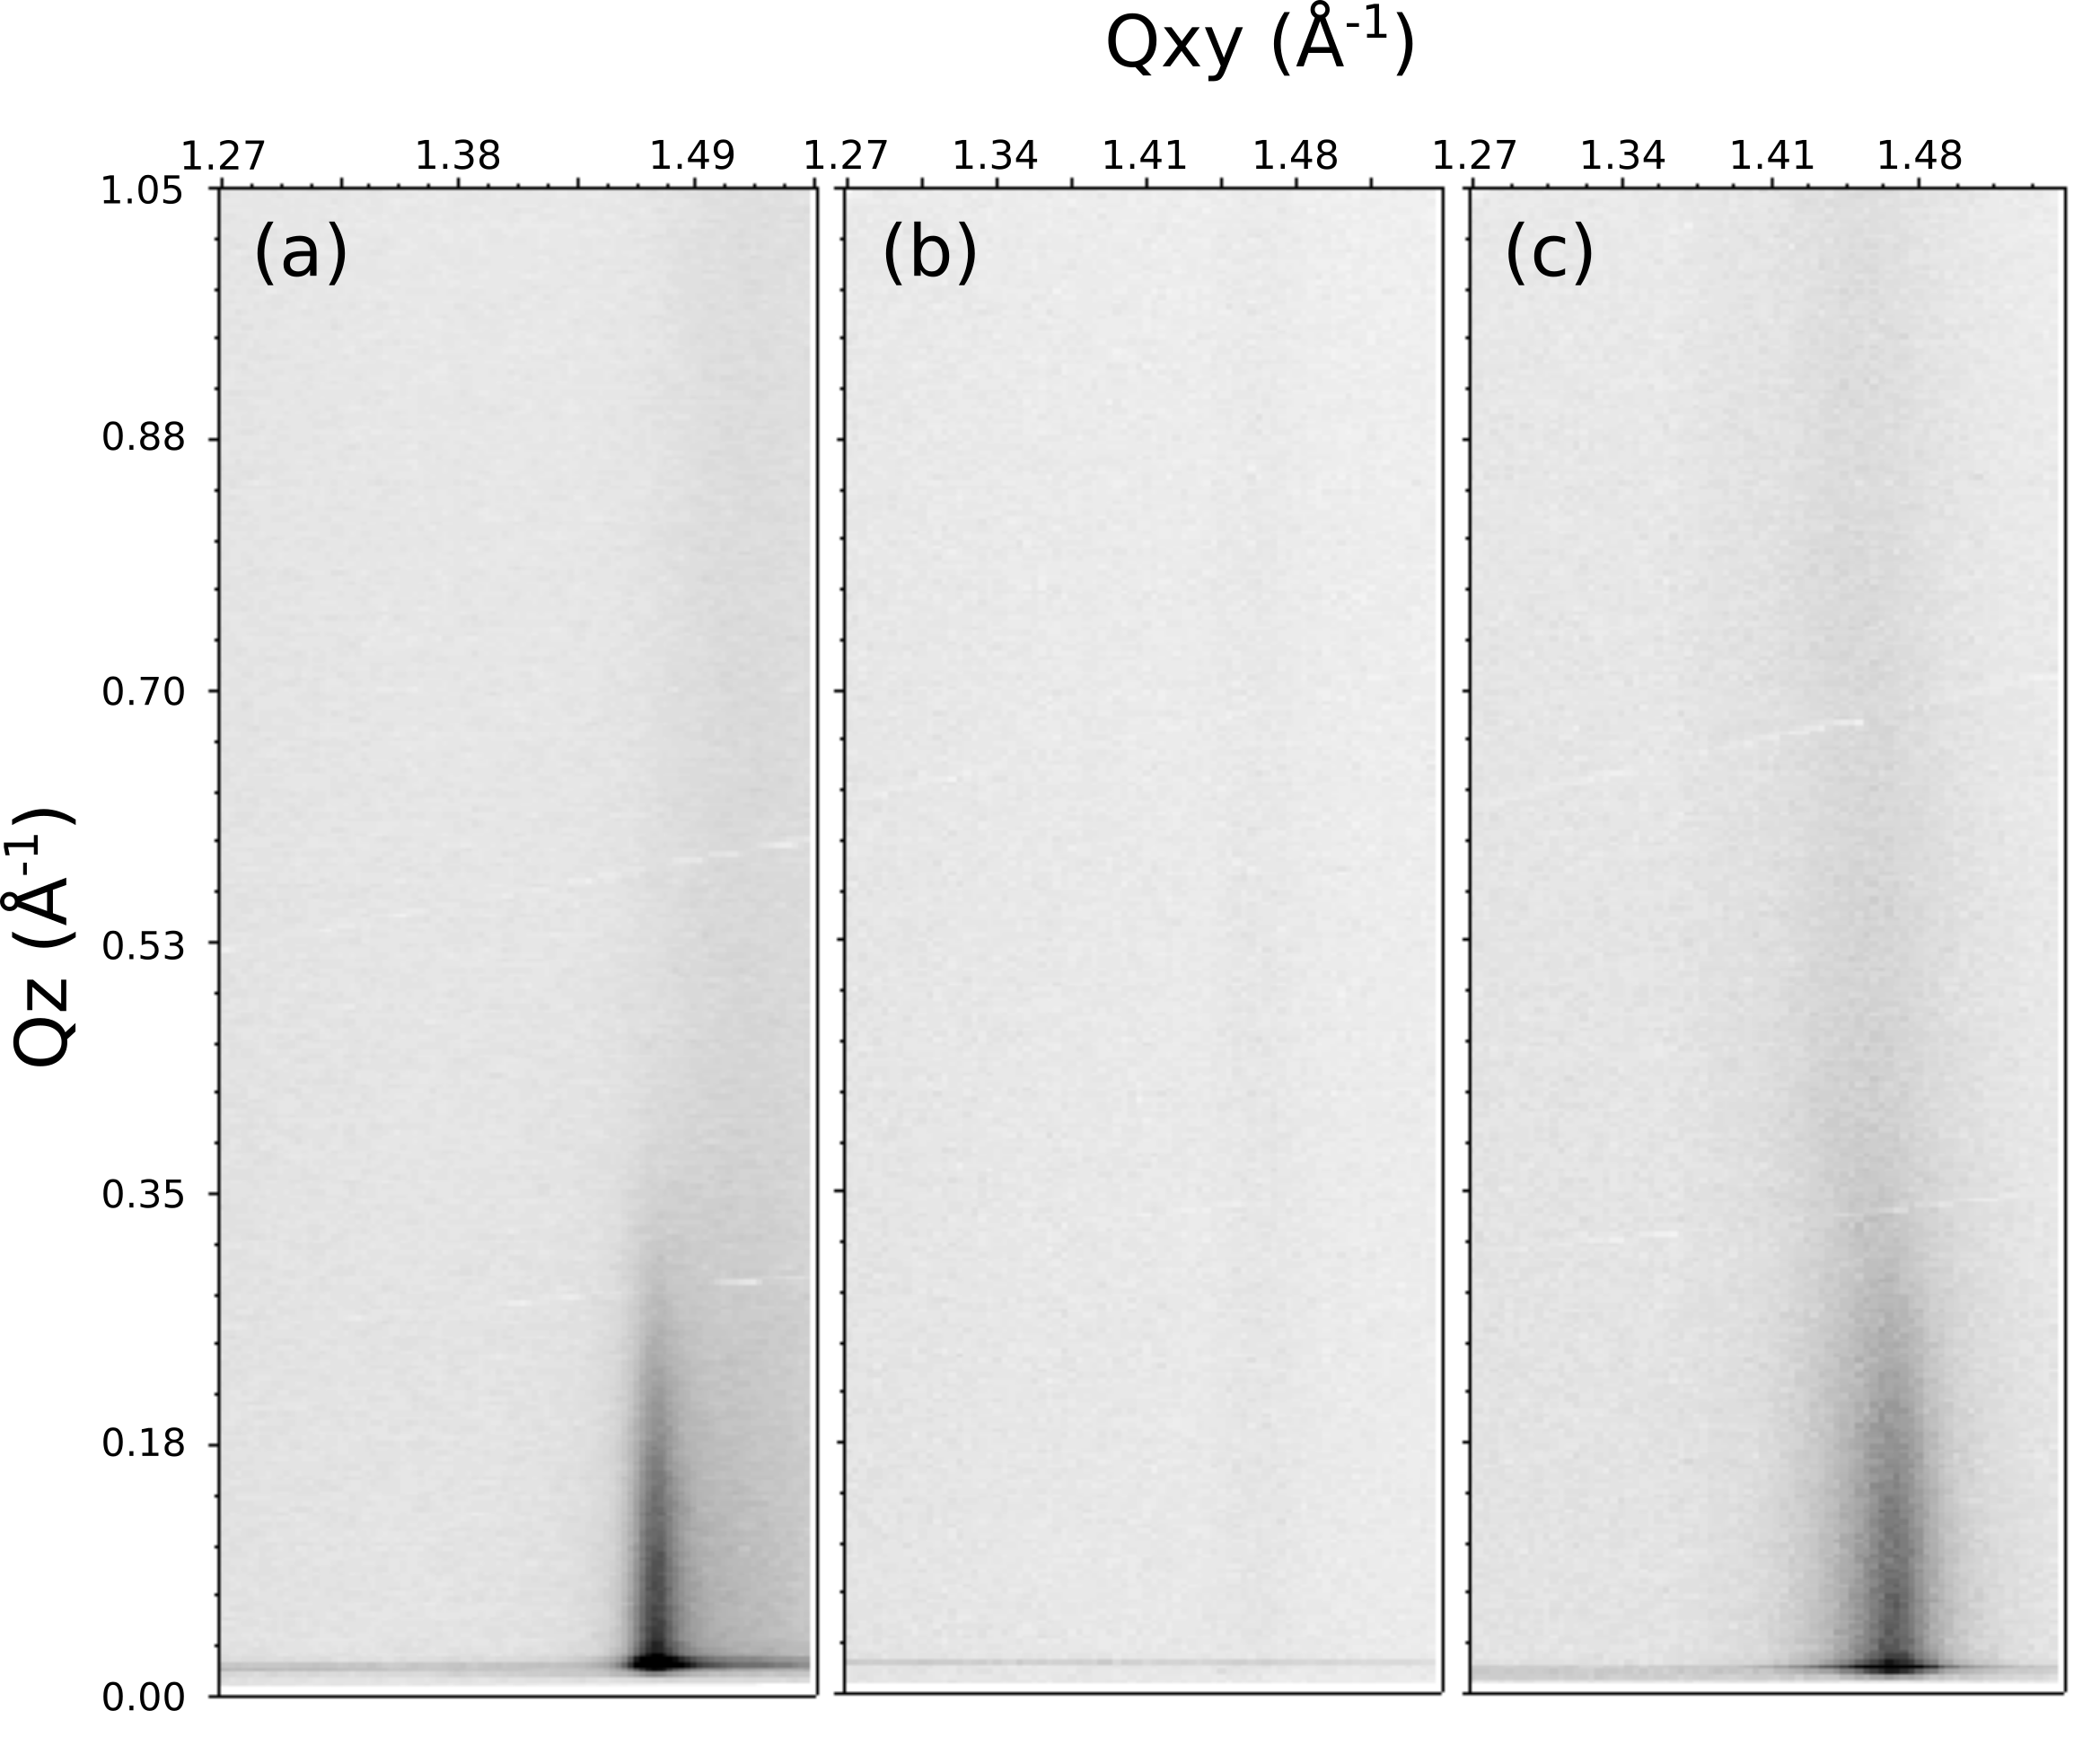
\includegraphics[width=0.6\textwidth]{reflectometry1/gixd}
    \caption{The GIXD patterns, where $Q_z$ is the scattering vector normal to the interface and $Q_{xy}$ is that in the plane of the interface; (a) DPPC at \SI{30}{\milli\newton\per\meter} and \SI{22}{\celsius}, (b) DMPC at \SI{30}{\milli\newton\per\meter} and \SI{22}{\celsius}, and (c) DMPC at \SI{30}{\milli\newton\per\meter} and \SI{7}{\celsius}.}
    \label{fig:gixd}
\end{figure}
%

Initially, this chemically-consistent modelling approach was applied only to the XRR data.
The tail layer thickness and interfacial roughness were allowed to vary independently across the surface pressures, while the other parameters were constrained as discussed above or held constant to the values given in Table~\ref{tab:invar}.
For each co-refinement of four XRR measurements, there were, in total, eleven degrees of freedom.
Throughout all of the analyses, the intensity scale factor was allowed to vary freely, while the background was constrained to the intensity at the largest $q$-value.

Following this, the head and tail group volumes, and the head layer thickness that were found from the XRR analysis were used as fixed variables for the refinement of the NR measurements.
This reduced the number of fitted parameters in the NR data to two, namely the thickness of the tail layer, $d_t$, and the interfacial roughness, $\sigma_{t,h,s}$, for the co-refinement of two datasets.
Table~\ref{tab:invar} also presents details of the scattering lengths and SLDs usedß for the NR refinement.
Again, the intensity scale factor was allowed to vary freely and the background constrained to the intensity at the largest $q$-value.

In both the XRR and the NR analysis, the refinement of the chemically-consistent model to the experimental data involved the transformation of the reflectometry calculated from the model and the data into $Rq^4$-space, such that the contribution of the Fresnel decay was removed \cite{gerelli_aurore_2016}.
The model was then optimised using the differential evolution method that is available within the \texttt{scipy} library \cite{jones_scipy_nodate}.
This refined the parameters to give the best fit to the data.
Markov chain Monte Carlo (MCMC) was then used to probe the search-space available to each parameter, given the experimental uncertainty of the data.
The MCMC sampling method used was Goodman \& Weare's Affine Invarient Ensemble \cite{goodman_ensemble_2010} as impliemented in the \texttt{emcee} package \cite{foreman-mackey_emcee_2013}.
This enabled the determination of the probability distribution for each of the parameters, and therefore the quantification of their inverse uncertainty, given the uncertainty in the experimental data.
A Shapiro-Wilk test \cite{shapiro_analysis_1965} was used to determine if the probability distribution function (PDF) fitted to a normal distrubition and therefore could be considered to have symmetric confidence intervals.
If the PDF failed the test the value was quoted with asymmetric confidence intervals, compared with the symmetric confidence intervals given for those that passed the Shapiro-Wilk test.
It is important to note that the PDFs and therefore the determined confidence intervals are not true confidence intervals, and account only for the uncertainty that is present in the data, i.e. they do not account for systematic uncertainty in the measurement technique.
In addition to determining parameter confidence intervals, it was also possible to use these probability distributions to understand the correlations present between the parameters and the impact this has on the fitting process.
The correlation was quantified using the Pearson correlation coefficient \cite{pearson_notes_1895}, a common statistical definition for the level of correlation present between two variables.
The Pearson correlation coefficient can have values that range from \numrange{-1}{1}, with a value of \num{-1} corresponding to a complete negative correlation (an increase in one variable is associated with a decrease in the other), while a value of \num{1} corresponds to a complete positive correlation (an increase in one variable is associated with a similar increase in the other), a value of \num{0} indicates no correlation between the two variables.
The MCMC sampling involved 200 walkers that were used for 1000 iterations, following a burn-in of 200 iterations.

\section{Results \& Discussion}
\subsection{X-ray reflectometry}
The chemically-consistent model was co-refined across XRR measurements at all four surface pressures for each phospholipid.
The resulting XRR profiles and associated SLD profiles are shown in Figure~\ref{fig:xrrref}.
Tables~\ref{tab:xrrref1}, \ref{tab:xrrref2}, \ref{tab:xrrref3}, and \ref{tab:xrrref4} gives the parameters for each of the phospholipids at each surface pressure measured, as well as the details fo $\phi_h$, as determined from Equation~\ref{equ:phih}.
%
\begin{figure}
    \centering
    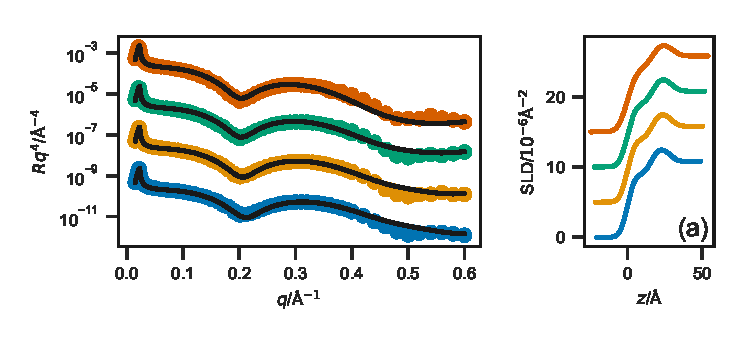
\includegraphics[width=0.80\textwidth]{reflectometry1/dppc_xray_ref_sld}
    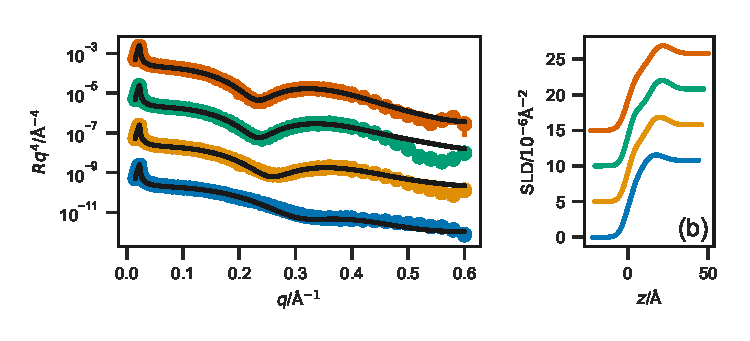
\includegraphics[width=0.80\textwidth]{reflectometry1/dmpc_xray_ref_sld}
    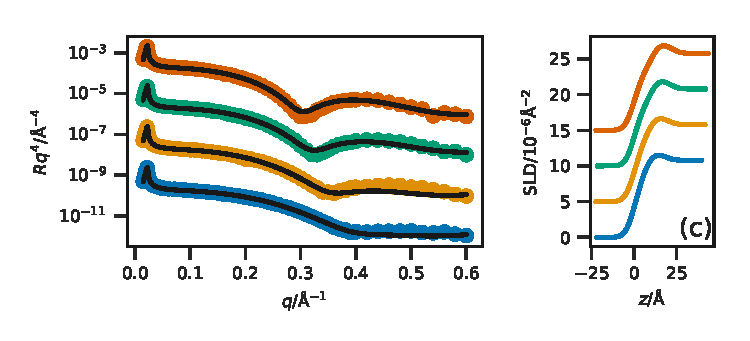
\includegraphics[width=0.80\textwidth]{reflectometry1/dlpc_xray_ref_sld}
    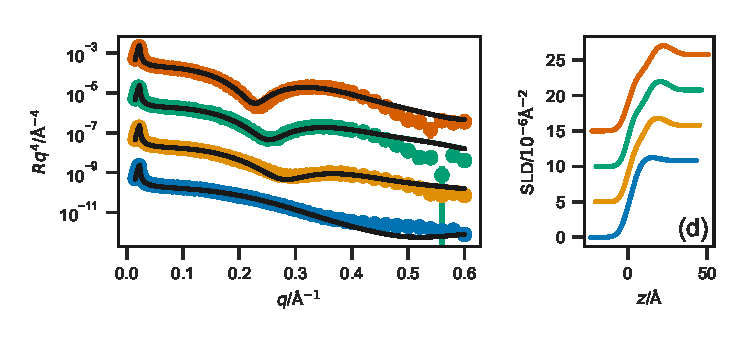
\includegraphics[width=0.80\textwidth]{reflectometry1/dmpg_xray_ref_sld}
    \caption{The XRR profiles (left) and SLD profiles (right) for each of the four phospholipids; (a) DPPC, (b) DMPC, (c) DLPC, and (d) DMPG, at the four measured surface pressures; increasing in surface pressure from blue, orange, green to red. The different surface pressure XRR profiles have been offset in the \emph{y}-axis by two orders of magnitude and the SLD profiles offset in the \emph{y}-axis by \SI{5e-6}{\per\angstrom\squared}, for clarity.}
    \label{fig:xrrref}
\end{figure}
%
%
\begin{table}
    \centering
    \small
    \caption{The best-fit values, and associated \SI{95}{\percent} confidence intervals for each of the varying parameters for each phospholipid at the lowest surface pressure measured from XRR. The values of $\phi_h$ were obtained from the appropriate use of Equation~\ref{equ:phih}.}
    \label{tab:xrrref1}
    \begin{tabular}{l | l l l l}
        \toprule
        Phospholipid & DPPC & DMPC & DLPC & DMPG \\
        Surface Pressure/\si{\milli\newton\per\meter} & 15 & 20 & 20 & 15 \\
        \midrule
        $V_t$/\si{\angstrom\cubed} & \input{output/reflectometry1/dppc_xray/dppc_xray-V_t} & \input{output/reflectometry1/dmpc_xray/dmpc_xray-V_t} & \input{output/reflectometry1/dlpc_xray/dlpc_xray-V_t} & \input{output/reflectometry1/dmpg_xray/dmpg_xray-V_t} \\
        $V_h$/\si{\angstrom\cubed} & \input{output/reflectometry1/dppc_xray/dppc_xray-V_h} & \input{output/reflectometry1/dmpc_xray/dmpc_xray-V_h} & \input{output/reflectometry1/dlpc_xray/dlpc_xray-V_h} & \input{output/reflectometry1/dmpg_xray/dmpg_xray-V_h} \\
        $d_h$/\si{\angstrom} & \input{output/reflectometry1/dppc_xray/dppc_xray-d_h} & \input{output/reflectometry1/dmpc_xray/dmpc_xray-d_h} & \input{output/reflectometry1/dlpc_xray/dlpc_xray-d_h} & \input{output/reflectometry1/dmpg_xray/dmpg_xray-d_h} \\
        \midrule
        $d_t$\si{\angstrom} & \input{output/reflectometry1/dppc_xray/dppc_xray-d_t_15} & \input{output/reflectometry1/dmpc_xray/dmpc_xray-d_t_20} & \input{output/reflectometry1/dlpc_xray/dlpc_xray-d_t_20} & \input{output/reflectometry1/dmpg_xray/dmpg_xray-d_t_15} \\
        $\sigma_{t,h,s}$/\si{\angstrom} & \input{output/reflectometry1/dppc_xray/dppc_xray_rough_15} & \input{output/reflectometry1/dmpc_xray/dmpc_xray_rough_20} & \input{output/reflectometry1/dlpc_xray/dlpc_xray_rough_20} & \input{output/reflectometry1/dmpg_xray/dmpg_xray_rough_15} \\
        \midrule
        $\phi_h$/$\times 10^{-2}$ & \input{output/reflectometry1/dppc_xray/dppc_xray-phih_15} & \input{output/reflectometry1/dmpc_xray/dmpc_xray-phih_20} & \input{output/reflectometry1/dlpc_xray/dlpc_xray-phih_20} & \input{output/reflectometry1/dmpg_xray/dmpg_xray-phih_15} \\
        \bottomrule
    \end{tabular}
\end{table}
%
%
\begin{table}
    \centering
    \small
    \caption{The best-fit values, and associated \SI{95}{\percent} confidence intervals for each of the varying parameters for each phospholipid at the second lowest surface pressure measured from XRR. The values of $\phi_h$ were obtained from the appropriate use of Equation~\ref{equ:phih}.}
    \label{tab:xrrref2}
    \begin{tabular}{l | l l l l}
        \toprule
        Phospholipid & DPPC & DMPC & DLPC & DMPG \\
        Surface Pressure/\si{\milli\newton\per\meter} & 20 & 25 & 25 & 20 \\
        \midrule
        $V_t$/\si{\angstrom\cubed} & \input{output/reflectometry1/dppc_xray/dppc_xray-V_t} & \input{output/reflectometry1/dmpc_xray/dmpc_xray-V_t} & \input{output/reflectometry1/dlpc_xray/dlpc_xray-V_t} & \input{output/reflectometry1/dmpg_xray/dmpg_xray-V_t} \\
        $V_h$/\si{\angstrom\cubed} & \input{output/reflectometry1/dppc_xray/dppc_xray-V_h} & \input{output/reflectometry1/dmpc_xray/dmpc_xray-V_h} & \input{output/reflectometry1/dlpc_xray/dlpc_xray-V_h} & \input{output/reflectometry1/dmpg_xray/dmpg_xray-V_h} \\
        $d_h$/\si{\angstrom} & \input{output/reflectometry1/dppc_xray/dppc_xray-d_h} & \input{output/reflectometry1/dmpc_xray/dmpc_xray-d_h} & \input{output/reflectometry1/dlpc_xray/dlpc_xray-d_h} & \input{output/reflectometry1/dmpg_xray/dmpg_xray-d_h} \\
        \midrule
        $d_t$\si{\angstrom} & \input{output/reflectometry1/dppc_xray/dppc_xray-d_t_20} & \input{output/reflectometry1/dmpc_xray/dmpc_xray-d_t_25} & \input{output/reflectometry1/dlpc_xray/dlpc_xray-d_t_25} & \input{output/reflectometry1/dmpg_xray/dmpg_xray-d_t_20} \\
        $\sigma_{t,h,s}$/\si{\angstrom} & \input{output/reflectometry1/dppc_xray/dppc_xray_rough_20} & \input{output/reflectometry1/dmpc_xray/dmpc_xray_rough_25} & \input{output/reflectometry1/dlpc_xray/dlpc_xray_rough_25} & \input{output/reflectometry1/dmpg_xray/dmpg_xray_rough_20} \\
        \midrule
        $\phi_h$/$\times 10^{-2}$ & \input{output/reflectometry1/dppc_xray/dppc_xray-phih_20} & \input{output/reflectometry1/dmpc_xray/dmpc_xray-phih_25} & \input{output/reflectometry1/dlpc_xray/dlpc_xray-phih_25} & \input{output/reflectometry1/dmpg_xray/dmpg_xray-phih_20} \\
        \bottomrule
    \end{tabular}
\end{table}
%
%
\begin{table}
    \centering
    \small
    \caption{The best-fit values, and associated \SI{95}{\percent} confidence intervals for each of the varying parameters for each phospholipid at the second highest surface pressure measured from XRR. The values of $\phi_h$ were obtained from the appropriate use of Equation~\ref{equ:phih}.}
    \label{tab:xrrref3}
    \begin{tabular}{l | l l l l}
        \toprule
        Phospholipid & DPPC & DMPC & DLPC & DMPG \\
        Surface Pressure/\si{\milli\newton\per\meter} & 25 & 30 & 30 & 25 \\
        \midrule
        $V_t$/\si{\angstrom\cubed} & \input{output/reflectometry1/dppc_xray/dppc_xray-V_t} & \input{output/reflectometry1/dmpc_xray/dmpc_xray-V_t} & \input{output/reflectometry1/dlpc_xray/dlpc_xray-V_t} & \input{output/reflectometry1/dmpg_xray/dmpg_xray-V_t} \\
        $V_h$/\si{\angstrom\cubed} & \input{output/reflectometry1/dppc_xray/dppc_xray-V_h} & \input{output/reflectometry1/dmpc_xray/dmpc_xray-V_h} & \input{output/reflectometry1/dlpc_xray/dlpc_xray-V_h} & \input{output/reflectometry1/dmpg_xray/dmpg_xray-V_h} \\
        $d_h$/\si{\angstrom} & \input{output/reflectometry1/dppc_xray/dppc_xray-d_h} & \input{output/reflectometry1/dmpc_xray/dmpc_xray-d_h} & \input{output/reflectometry1/dlpc_xray/dlpc_xray-d_h} & \input{output/reflectometry1/dmpg_xray/dmpg_xray-d_h} \\
        \midrule
        $d_t$\si{\angstrom} & \input{output/reflectometry1/dppc_xray/dppc_xray-d_t_25} & \input{output/reflectometry1/dmpc_xray/dmpc_xray-d_t_30} & \input{output/reflectometry1/dlpc_xray/dlpc_xray-d_t_30} & \input{output/reflectometry1/dmpg_xray/dmpg_xray-d_t_25} \\
        $\sigma_{t,h,s}$/\si{\angstrom} & \input{output/reflectometry1/dppc_xray/dppc_xray_rough_25} & \input{output/reflectometry1/dmpc_xray/dmpc_xray_rough_30} & \input{output/reflectometry1/dlpc_xray/dlpc_xray_rough_30} & \input{output/reflectometry1/dmpg_xray/dmpg_xray_rough_25} \\
        \midrule
        $\phi_h$/$\times 10^{-2}$ & \input{output/reflectometry1/dppc_xray/dppc_xray-phih_25} & \input{output/reflectometry1/dmpc_xray/dmpc_xray-phih_30} & \input{output/reflectometry1/dlpc_xray/dlpc_xray-phih_30} & \input{output/reflectometry1/dmpg_xray/dmpg_xray-phih_25} \\
        \bottomrule
    \end{tabular}
\end{table}
%
%
\begin{table}
    \centering
    \small
    \caption{The best-fit values, and associated \SI{95}{\percent} confidence intervals for each of the varying parameters for each phospholipid at the highest surface pressure measured from XRR. The values of $\phi_h$ were obtained from the appropriate use of Equation~\ref{equ:phih}.}
    \label{tab:xrrref4}
    \begin{tabular}{l | l l l l}
        \toprule
        Phospholipid & DPPC & DMPC & DLPC & DMPG \\
        Surface Pressure/\si{\milli\newton\per\meter} & 30 & 40 & 35 & 30 \\
        \midrule
        $V_t$/\si{\angstrom\cubed} & \input{output/reflectometry1/dppc_xray/dppc_xray-V_t} & \input{output/reflectometry1/dmpc_xray/dmpc_xray-V_t} & \input{output/reflectometry1/dlpc_xray/dlpc_xray-V_t} & \input{output/reflectometry1/dmpg_xray/dmpg_xray-V_t} \\
        $V_h$/\si{\angstrom\cubed} & \input{output/reflectometry1/dppc_xray/dppc_xray-V_h} & \input{output/reflectometry1/dmpc_xray/dmpc_xray-V_h} & \input{output/reflectometry1/dlpc_xray/dlpc_xray-V_h} & \input{output/reflectometry1/dmpg_xray/dmpg_xray-V_h} \\
        $d_h$/\si{\angstrom} & \input{output/reflectometry1/dppc_xray/dppc_xray-d_h} & \input{output/reflectometry1/dmpc_xray/dmpc_xray-d_h} & \input{output/reflectometry1/dlpc_xray/dlpc_xray-d_h} & \input{output/reflectometry1/dmpg_xray/dmpg_xray-d_h} \\
        \midrule
        $d_t$\si{\angstrom} & \input{output/reflectometry1/dppc_xray/dppc_xray-d_t_30} & \input{output/reflectometry1/dmpc_xray/dmpc_xray-d_t_40} & \input{output/reflectometry1/dlpc_xray/dlpc_xray-d_t_35} & \input{output/reflectometry1/dmpg_xray/dmpg_xray-d_t_30} \\
        $\sigma_{t,h,s}$/\si{\angstrom} & \input{output/reflectometry1/dppc_xray/dppc_xray_rough_30} & \input{output/reflectometry1/dmpc_xray/dmpc_xray_rough_40} & \input{output/reflectometry1/dlpc_xray/dlpc_xray_rough_35} & \input{output/reflectometry1/dmpg_xray/dmpg_xray_rough_30} \\
        \midrule
        $\phi_h$/$\times 10^{-2}$ & \input{output/reflectometry1/dppc_xray/dppc_xray-phih_30} & \input{output/reflectometry1/dmpc_xray/dmpc_xray-phih_40} & \input{output/reflectometry1/dlpc_xray/dlpc_xray-phih_35} & \input{output/reflectometry1/dmpg_xray/dmpg_xray-phih_30} \\
        \bottomrule
    \end{tabular}
\end{table}
%

Following the structural determination of the monolayer from the XRR measurements.
NR was used to confirm the values of the head and tail group volumes that had been determined.
The resulting NR profiles and associated SLD profiles, at both surface pressures measured can be found in Figure~\ref{fig:nrref}.
Table~\ref{tab:nrref} gives the parameters as determined from the NR measurements, along with $\phi_h$ as determined from Equation~\ref{equ:phih}.
%
\begin{figure}
    \centering
    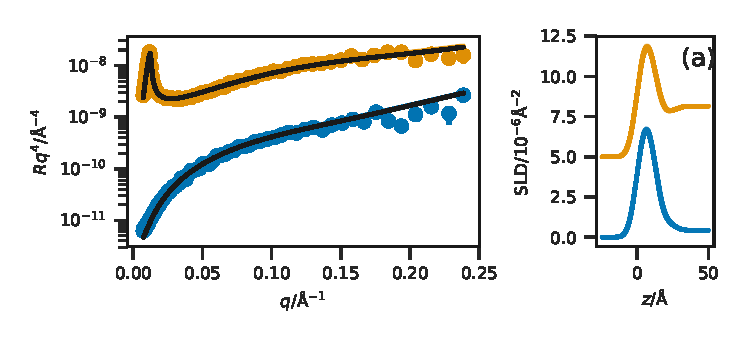
\includegraphics[width=0.80\textwidth]{reflectometry1/dppc_neutron_15_ref_sld}
    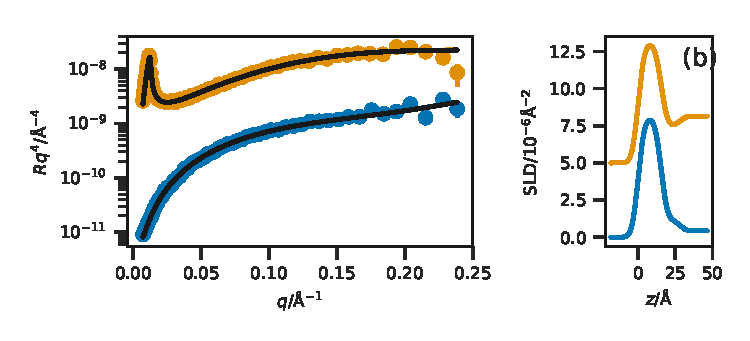
\includegraphics[width=0.80\textwidth]{reflectometry1/dppc_neutron_20_ref_sld}
    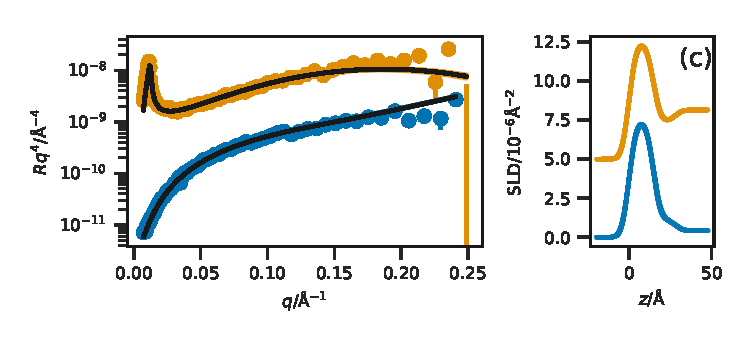
\includegraphics[width=0.80\textwidth]{reflectometry1/dmpc_neutron_20_ref_sld}
    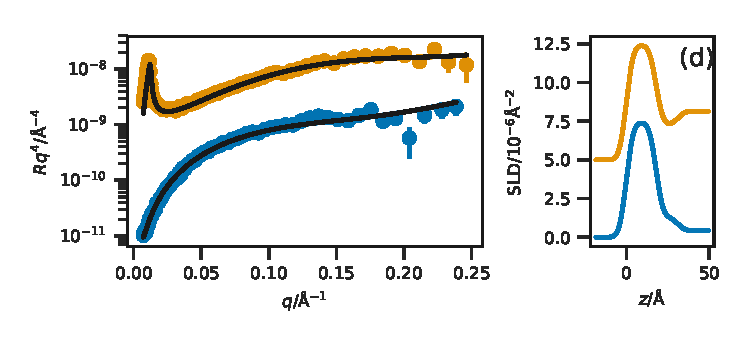
\includegraphics[width=0.80\textwidth]{reflectometry1/dmpc_neutron_25_ref_sld}
    \caption{The NR profiles (left) and SLD profiles (right) for each of the four phospholipids; (a) DPPC at \SI{15}{\milli\newton\per\meter}, (b) DPPC at \SI{20}{\milli\newton\per\meter}, (c) DMPC at \SI{20}{\milli\newton\per\meter}, and (d) DMPC at \SI{25}{\milli\newton\per\meter}, where the blue data indicates the h-DES contrast, while the orange is the hd-DES. The different surface pressure XRR profiles have been offset in the \emph{y}-axis by an order of magnitude and the SLD profiles offset in the \emph{y}-axis by \SI{5e-6}{\per\angstrom\squared}, for clarity.}
    \label{fig:nrref}
\end{figure}
%
%
\begin{table}
    \centering
    \small
    \caption{The best-fit values, and associated \SI{95}{\percent} confidence intervals for each of the varying parameters for each phospholipid at the each surface pressure from NR. The values of $\phi_h$ were obtained from the appropriate use of Equation~\ref{equ:phih}.}
    \label{tab:nrref}
    \begin{tabular}{l | l l l l}
        \toprule
        Phospholipid & DPPC & DPPC & DMPC & DMPC \\
        Surface Pressure/\si{\milli\newton\per\meter} & 15 & 20 & 20 & 25 \\
        \midrule
        $d_t$\si{\angstrom} & \input{output/reflectometry1/dppc_neutron/dppc_neutron_15-d_t_15} & \input{output/reflectometry1/dppc_neutron/dppc_neutron_20-d_t_20} & \input{output/reflectometry1/dmpc_neutron/dmpc_neutron_20-d_t_20} & \input{output/reflectometry1/dmpc_neutron/dmpc_neutron_25-d_t_25} \\
        $\sigma_{t,h,s}$/\si{\angstrom} & \input{output/reflectometry1/dppc_neutron/dppc_neutron_15_rough_15} & \input{output/reflectometry1/dppc_neutron/dppc_neutron_20_rough_20} & \input{output/reflectometry1/dmpc_neutron/dmpc_neutron_20_rough_20} & \input{output/reflectometry1/dmpc_neutron/dmpc_neutron_25_rough_25} \\
        \midrule
        $\phi_h$/$\times 10^{-2}$ & \input{output/reflectometry1/dppc_neutron/dppc_neutron_15-phih_15} & \input{output/reflectometry1/dppc_neutron/dppc_neutron_20-phih_20} & \input{output/reflectometry1/dmpc_neutron/dmpc_neutron_20-phih_20} & \input{output/reflectometry1/dmpc_neutron/dmpc_neutron_25-phih_25} \\
        \bottomrule
    \end{tabular}
\end{table}
%

\subsection{Effect of compression on the monolayer thickness}
From Tables~\ref{tab:xrrref1}, \ref{tab:xrrref2}, \ref{tab:xrrref3}, \ref{tab:xrrref4}, and \ref{tab:nrref}, we can see that, as expected and shown in previous work \cite{mohwald_phospholipid_1990,vaknin_structural_1991}, the thickness of the tail layer increases as the number of carbon atoms in the tail chain increases.
Furthermore, the thickness of the tail layers determined here agrees well with values found for water-analoguyes; \input{output/reflectometry1/dmpc_xray/dmpc_xray-d_t_30}\si{\angstrom} at \SI{30}{\milli\newton\per\meter} in DES compared with \SI{15.8}{\angstrom} at \SI{30}{\milli\newton\per\meter} in water for DMPC, and \input{output/reflectometry1/dppc_xray/dppc_xray-d_t_30}\si{\angstrom} at \SI{30}{\milli\newton\per\meter} in DES compared with \SI{16.7}{\angstrom} at \SI{40}{\milli\newton\per\meter} in water for DPPC.

The variation of the tail layer thickness in the models with surface pressure is given for each phospholipid in Figure~\ref{fig:dtphi}.
For all of the phospholipids, as the surface pressure increases, the thickness of the tail layer also increases to a point before plateauing; for DPPC this occurs at \SI{20}{\milli\newton\per\meter}, DMPC at \SI{30}{\milli\newton\per\meter}, and for DMPG and DLPC can be assumed to be at higher pressures than those studied.
This relationship of increasing tail layer thickness with increasing surface pressure has been noted previously for DMPC \cite{bayerl_specular_1990} and DPPC \cite{campbell_structure_2018} at the air-water interface.
This can be easily understood as the angle of the tail group with respect to the surface normal decreasing as the surface pressure increases.
%
\begin{figure}
    \centering
    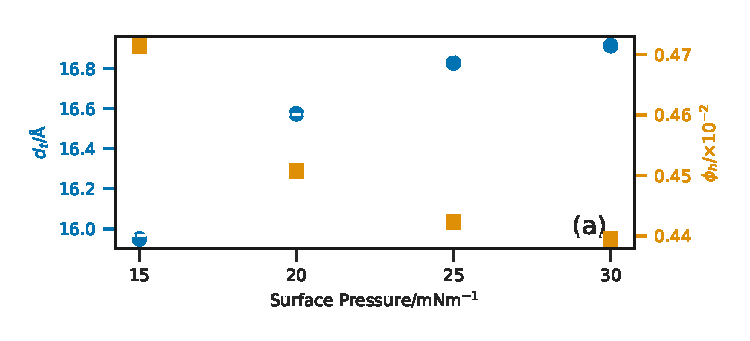
\includegraphics[width=0.8\textwidth]{reflectometry1/dppc_xray_dt_phi}
    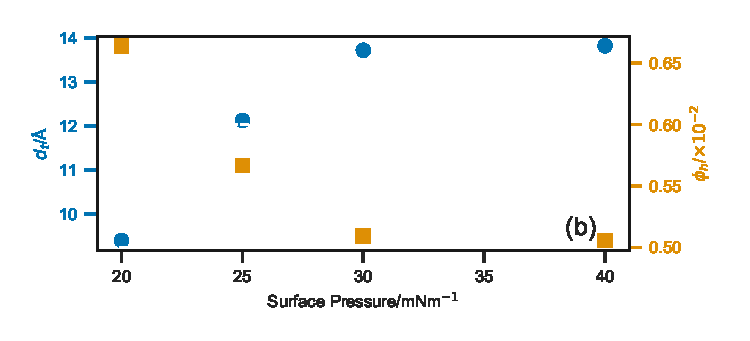
\includegraphics[width=0.8\textwidth]{reflectometry1/dmpc_xray_dt_phi}
    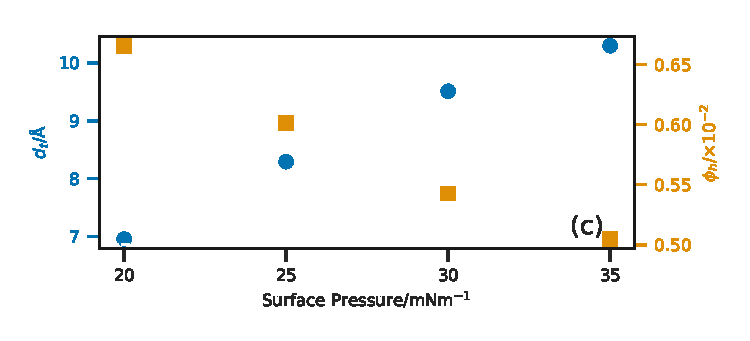
\includegraphics[width=0.8\textwidth]{reflectometry1/dlpc_xray_dt_phi}
    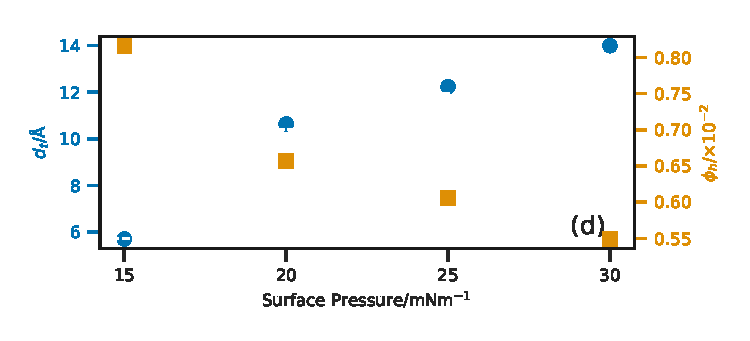
\includegraphics[width=0.8\textwidth]{reflectometry1/dmpg_xray_dt_phi}
    \caption{The variation of $d_t$ (blue circles) and $\phi_h$ (orange squares) with surface pressures for each of the four phospholipids; (a) DPPC, (b) DMPC, (c) DLPC, and (d) DMPG.}
    \label{fig:dtphi}
\end{figure}
%

\subsection{Effect of compressure on solvent fraction}
In Figure~\ref{fig:dtphi}, it is clear that for all four phospholipids, as the surface pressure is increased there is a corresponding reduction in the volume fraction of solvent in the phospholipid head layer,
This can be rationalised by considering that when the surface pressure is increased, there is a corresponding increase in surface concentration, hence the free volume available to the solvent is less.
A similar effect has been observed when increase the surface pressure from \SI{11}{\milli\newton\per\meter} to \SI{31}{\milli\newton\per\meter} for a mixed DMPC/DMPG monolayer at the air-water interface \cite{bayerl_specular_1990}.

\subsection{Effect of compression on the lipid tail component volumes}
It can be seen from comparing Table~\ref{tab:water} with Tables~\ref{tab:xrrref1}, \ref{tab:xrrref2}, \ref{tab:xrrref3}, and \ref{tab:xrrref4} that the volume of the phospholipid tails are significantly lower in the current measurement than found previously, by other techniques.
It is unlikely that this is a result of the DES subphase, due to the hydrophobic nature of these tail groups.
However, this reduction has been shown previously \cite{campbell_structure_2018}, where it was rationalised by the compaction of the monolayer at elevated surface pressure.
In that work, the optimal value for the tail group volume of DPPC was found to be \SI{772}{\angstrom\cubed} at a surface pressure of \SI{35}{\milli\newton\per\meter}, which agree well with the value of \input{output/reflectometry1/dppc_xray/dppc_xray-V_t.tex}\si{\angstrom\cubed} found in this work at surface pressures of \SIlist{15;20;25;30}{\milli\newton\per\meter}.
This reduction was found to be between \SIrange{8}{12}{\percent} for DPPC, DMPC, DLPC when compared with the literature sources at \SIlist{24;30}{\celsius}.
This is close to the maximum compression percentage of \SI{15}{\percent} noted by Small \cite{small_lateral_1984}.
DMPG shows a small increase in the tail volume when compared with the literature value, albeit at a higher temperature.
However, this value agrees well with that found for DMPC which shares the same tail structure.

\subsection{Solvent effect on the lipid head group volume}
Tables~\ref{tab:xrrref1}, \ref{tab:xrrref2}, \ref{tab:xrrref3}, and \ref{tab:xrrref4} give the best-fit values for the head group volumes for each of phospholipids investigated.
Ths three phospholipids with the PC head group are consistent, giving values of \SI{\sim 330}{\angstrom\cubed}, regardless of the tail group.
This agrees well with the values found for the same head component in water, shown in Table~\ref{tab:water}.
Interestingly, the head group volume determined for the PG containing phospholipid is similar to that for the PC head group, with a value of \input{output/reflectometry1/dmpg_xray/dmpg_xray-V_h.tex}.
The PG head group volume in water, from either DMPG using differential vibrating tube densimetry \cite{pan_molecular_2012} or POPG using molecular dynamics simulations \cite{kucerka_scattering_2012}, is noticeably smaller.
This indicates that there may be some effect arising from the solvation of the PG component in the choline chloride:glycerol DES.
However, this is not conclusive as it has only been shown for a single PG-lipid at the air-DES interface.

The major difference between the two head groups is the fact that the PG head group is negatively charged whereas the PC head group is zwitterionic.
It has been shown previously that the conformation for the PC component is folded in water \cite{gillams_comparative_2016}, due to the interaction between the positively-charged ammonium and negatively-charged phosphate groups.
A similar structure may occur for the PG head group, with an interaction between the partially positively-charged alcoholic hydrogen atoms and the negatively-charged phosphate group.
However, for PG, such an interaction would be weaker than that observed in the PC group.
Therefore, this observed increase found for the PG head group volume in DES when compared with water may be due to the unfolding of the PG head conformation.
This unfolding would be made possible by the charged nature of the solvent, providing a greater screening effect for the PG head group than present in water.
This effect may not be observed for the PC head group as the formal charges present result in a stronger electrostatic interaction that may not be screened sufficiently by the DES.
It is anticipated that this unfolding would result in an increase in the thickness of the lipid head layer.
Previously, DPPG has been reported to have a head layer thickness of \SI{10.3\pm0.4}{\angstrom} at \SI{22}{\milli\newton\per\meter} from neutron reflectometry measurements \cite{clifton_role_2012}, which is slightly less than the \input{output/reflectometry1/dmpg_xray/dmpg_xray-d_h.tex}\si{\angstrom} determined in this work, further suggesting that the unfolding of the PG head group may be occuring in the presence of the DES.

\subsection{Analysis of neutron reflectometry}
The ability to fit NR data in Figure~\ref{fig:nrref} indicated that the values found for the head and tail groups are consistent between the pair of measurements for the same systems.
It is clear, that again stable monolayers of the phospholipids are forming at the air-DES interface and that the volume determined by XRR measurements are robust enough to be used in the modelling of NR data.
Furthermore, as shown in Table~\ref{tab:nrref}, the trends observed with increasing surface pressure in the XRR models, pertaining to a responsive increase in tail thickness and a decrease in solvent concentration in the head layer are consistent with that found with the NR analysis.

\subsection{Utility of Markov chain Monte Carlo sampling}
The use of MCMC sampling enabled the inverse uncertainties for each of the fitted parameters to be determined as a confidence interval from the PDFs shown in Figures~\ref{fig:dppcpdfs}, \ref{fig:dmpcpdfs}, \ref{fig:dlpcpdfs}, \ref{fig:dmpgpdfs}, and \ref{fig:nrpdfs}.
These confidence intervals are useful for understanding the probability of the given value, however as discussed in Section~\ref{refl1:anal} these intervals only represent the uncertainty in the experimental data and do not account for systematic uncertainty present in the measurement method.
%
\begin{figure}
    \centering
    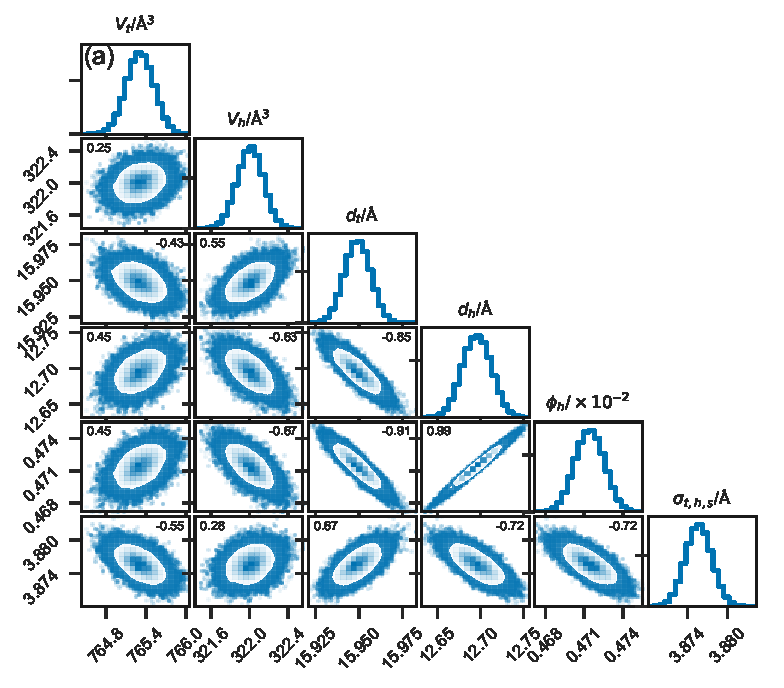
\includegraphics[width=0.49\textwidth]{reflectometry1/dppc_xray_sp_15_pdf}
    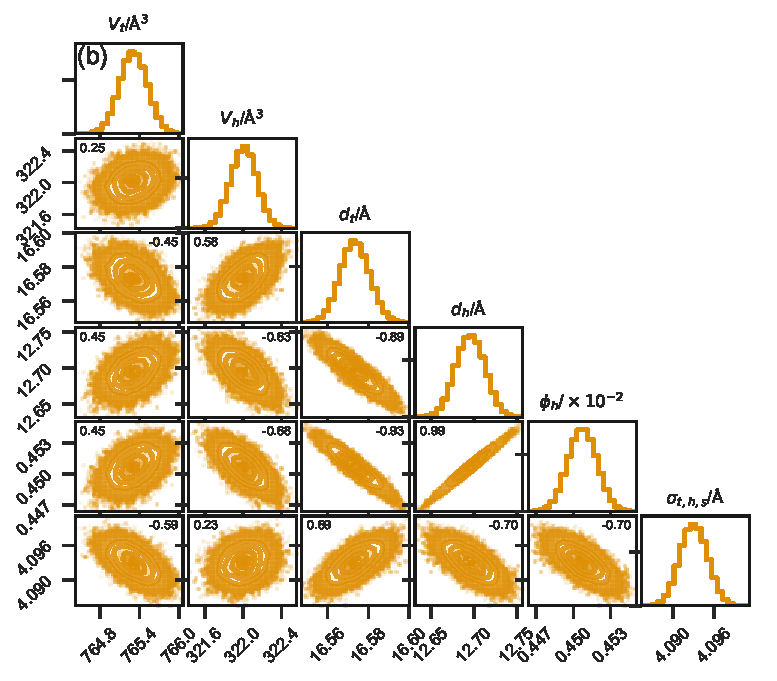
\includegraphics[width=0.49\textwidth]{reflectometry1/dppc_xray_sp_20_pdf} \\
    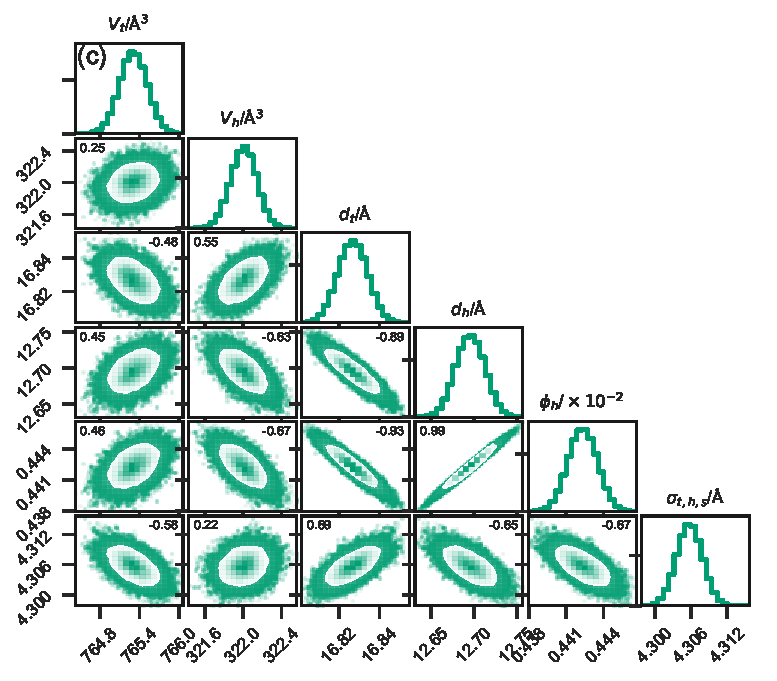
\includegraphics[width=0.49\textwidth]{reflectometry1/dppc_xray_sp_25_pdf}
    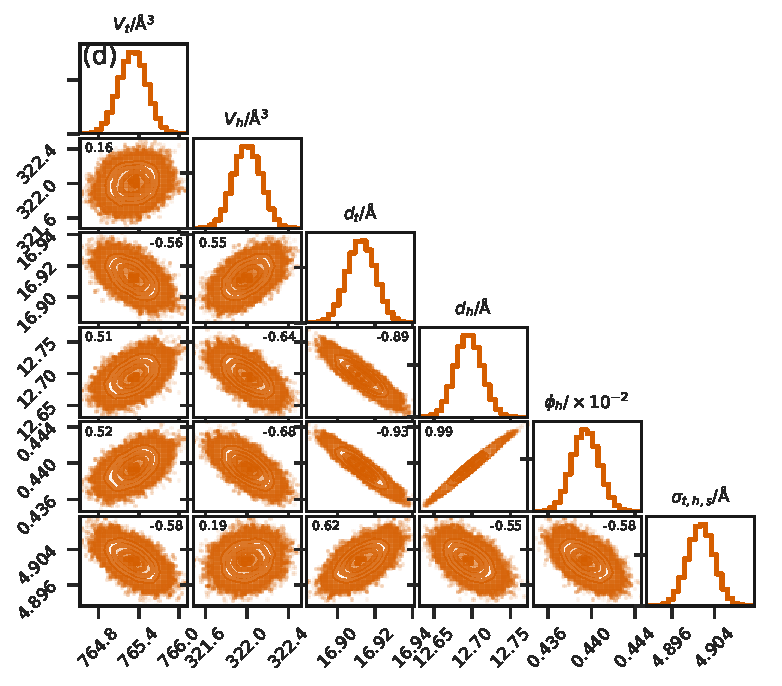
\includegraphics[width=0.49\textwidth]{reflectometry1/dppc_xray_sp_30_pdf}
    \caption{The probability distribution functions from the chemically-consistent modelling of DPPC; (a) at \SI{15}{\milli\newton\per\meter}, (b) at \SI{20}{\milli\newton\per\meter}, (c) at \SI{25}{\milli\newton\per\meter}, (d) at \SI{30}{\milli\newton\per\meter}. The Pearson correlation coefficient for each pair of parameters is given in the top corner of each two-dimensional PDF.}
    \label{fig:dppcpdfs}
\end{figure}
%
%
\begin{figure}
    \centering
    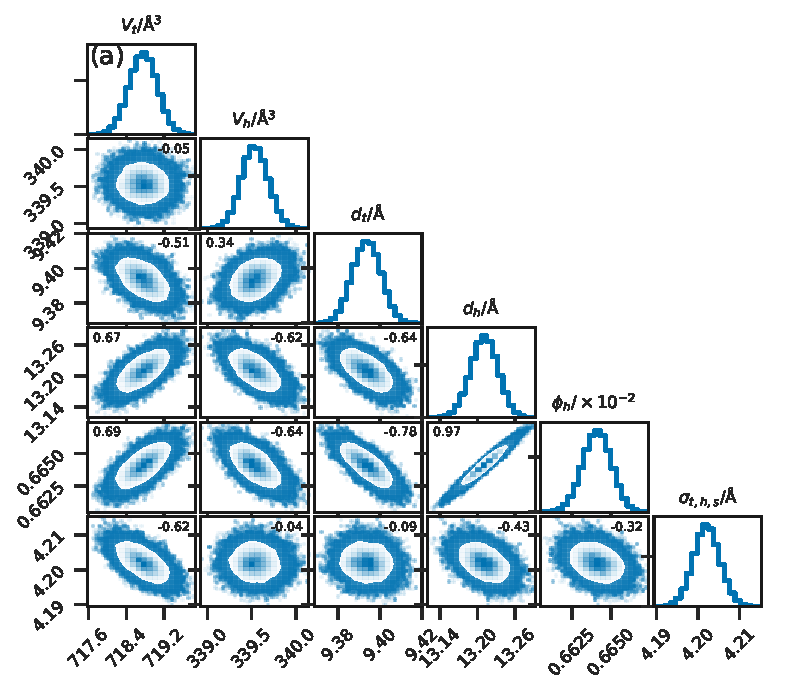
\includegraphics[width=0.49\textwidth]{reflectometry1/dmpc_xray_sp_20_pdf}
    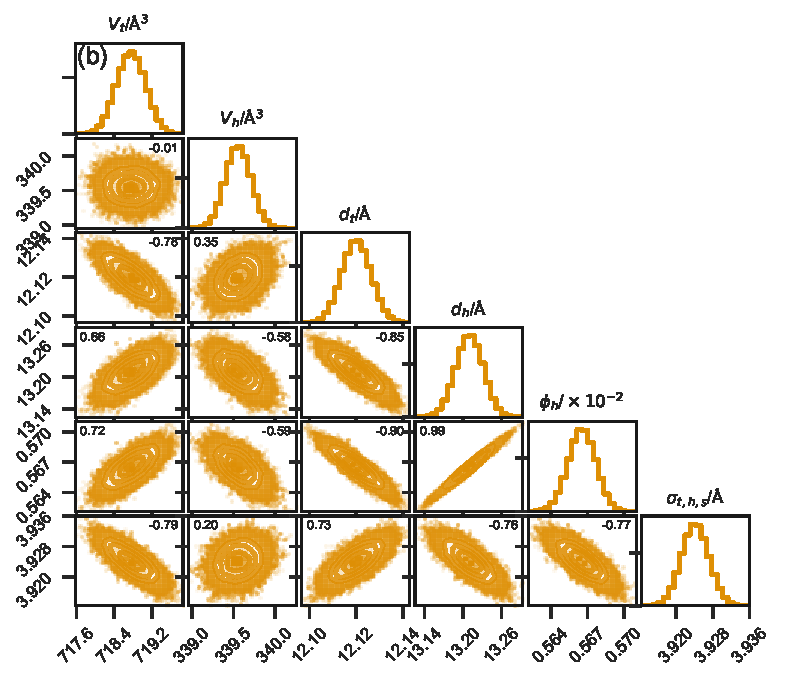
\includegraphics[width=0.49\textwidth]{reflectometry1/dmpc_xray_sp_25_pdf} \\
    \includegraphics[width=0.49\textwidth]{reflectometry1/dmpc_xray_sp_30_pdf}
    \includegraphics[width=0.49\textwidth]{reflectometry1/dmpc_xray_sp_40_pdf}
    \caption{The probability distribution functions from the chemically-consistent modelling of DMPC; (a) at \SI{20}{\milli\newton\per\meter}, (b) at \SI{25}{\milli\newton\per\meter}, (c) at \SI{30}{\milli\newton\per\meter}, (d) at \SI{40}{\milli\newton\per\meter}. The Pearson correlation coefficient for each pair of parameters is given in the top corner of each two-dimensional PDF.}
    \label{fig:dmpcpdfs}
\end{figure}
%
%
\begin{figure}
    \centering
    \includegraphics[width=0.49\textwidth]{reflectometry1/dlpc_xray_sp_20_pdf}
    \includegraphics[width=0.49\textwidth]{reflectometry1/dlpc_xray_sp_25_pdf} \\
    \includegraphics[width=0.49\textwidth]{reflectometry1/dlpc_xray_sp_30_pdf}
    \includegraphics[width=0.49\textwidth]{reflectometry1/dlpc_xray_sp_35_pdf}
    \caption{The probability distribution functions from the chemically-consistent modelling of DLPC; (a) at \SI{20}{\milli\newton\per\meter}, (b) at \SI{25}{\milli\newton\per\meter}, (c) at \SI{30}{\milli\newton\per\meter}, (d) at \SI{35}{\milli\newton\per\meter}. The Pearson correlation coefficient for each pair of parameters is given in the top corner of each two-dimensional PDF.}
    \label{fig:dlpcpdfs}
\end{figure}
%
%
\begin{figure}
    \centering
    \includegraphics[width=0.49\textwidth]{reflectometry1/dmpg_xray_sp_15_pdf}
    \includegraphics[width=0.49\textwidth]{reflectometry1/dmpg_xray_sp_20_pdf} \\
    \includegraphics[width=0.49\textwidth]{reflectometry1/dmpg_xray_sp_25_pdf}
    \includegraphics[width=0.49\textwidth]{reflectometry1/dmpg_xray_sp_30_pdf}
    \caption{The probability distribution functions from the chemically-consistent modelling of DMPG; (a) at \SI{15}{\milli\newton\per\meter}, (b) at \SI{20}{\milli\newton\per\meter}, (c) at \SI{25}{\milli\newton\per\meter}, (d) at \SI{30}{\milli\newton\per\meter}. The Pearson correlation coefficient for each pair of parameters is given in the top corner of each two-dimensional PDF.}
    \label{fig:dmpgpdfs}
\end{figure}
%
%
\begin{figure}
    \centering
    \includegraphics[width=0.49\textwidth]{reflectometry1/dppc_neutron_15_pdf}
    \includegraphics[width=0.49\textwidth]{reflectometry1/dppc_neutron_20_pdf} \\
    \includegraphics[width=0.49\textwidth]{reflectometry1/dmpc_neutron_20_pdf}
    \includegraphics[width=0.49\textwidth]{reflectometry1/dmpc_neutron_25_pdf}
    \caption{The probability distribution functions from the chemically-consistent modelling of the NR data; (a) DPPC at \SI{15}{\milli\newton\per\meter}, (b) DPPC at \SI{20}{\milli\newton\per\meter}, (c) DMPC at \SI{20}{\milli\newton\per\meter}, and (d) DMPC at \SI{25}{\milli\newton\per\meter}. The Pearson correlation coefficient for each pair of parameters is given in the top corner of each two-dimensional PDF.}
    \label{fig:nrpdfs}
\end{figure}
%

The sums of the magnitudes of the Pearson correlation coefficients for each PC-containing phospholipids at each surface pressures are given in Figure~\ref{fig:pear}.
From this figure, it is clear that there is a relationship between the phospholipid and the correlation present in the reflectometry model.
This is the effect of the reduction in the phospholipid length from DPPC to DLPC, and that a corresponding decrease is not observed for the interfacial roughness.
Therefore, the boundary between phospholipid head and tail layers is less well defined, this can be observed by investigating the SLD profiles in Figure~\ref{fig:xrrref}.
Furthermore, the magnitude of the Pearson correlation between the head and tail thicknesses increases with increasing tail length; from $\input{output/reflectometry1/dppc_xray/dppc_p_d_t_d_h_sp30.txt}$ for DPPC, to $\input{output/reflectometry1/dmpc_xray/dmpc_p_d_t_d_h_sp30.txt}$ for DMPC, to $\input{output/reflectometry1/dlpc_xray/dlpc_p_d_t_d_h_sp30.txt}$ for DLPC, each at \SI{30}{\milli\newton\per\meter}.
Indicating that as the phospholipid tail length decreases the negative correlation between the head and tail layers increases to the point for DLPC where the two variables are almost completely correlated and the boundary between the tail is nearly nonexistent.
%
\begin{figure}
    \centering
    \includegraphics[width=0.85\textwidth]{reflectometry1/pear}
    \caption{The sum of the magnitudes for each of the Pearson correlation coefficients for each of the PC-containing lipids.}
    \label{fig:pear}
\end{figure}
%

There is also a substantial positive correlation present for all of the datasets between the phospholipid head layer thickness and the volume fraction of solvent in the head layer.
This correlation can be rationalised as a result of the SLD of the solvent and the head layer (which is much as \SI{78}{\percent} solvent by volume) being similar, and therefore the boundary between the head layer and the solvent is also poorly defined.
A significant correlation such as this is unavoidable, without considering the use of many neutron contrasts for both the phospholipid and the solvent, due to the solvophilic nature of the head groups.

\section{Conclusions}
Stable PC and PG lipid monolayers were observed and characterised on an ionic solvent surface.
Until the emergence of ionic liquids and DES, only a limited number of molecular solvents exhibited the ability to promote self-assembly and only water and formamide among those had previously demonstrated the formation of phospholipid monolayers at the air-liquid interface.\autocite{mohwald_phospholipid_1990,graner_phospholipidic_1995}

For the first time, a physically and chemically-consistent reflectometry modelling approach was used to co-refine XRR measurements at different surface pressures.
This enabled modelling without the need to constrain the head and tail group volumes, enabling these parameters to vary freely to account for any variation occurring due to the elevated surface pressures used or the presence of a non-aqueous solvent, compared to the commonly applied literature values.
This allows a significant difference in the PG head group volume to be observed; having a larger volume than observed for the same system in water.
This suggests that the transfer of phospholipids to a DES is not just a simple substitution of the subphase.
In this specific case, we have proposed an explanation based on the dissociation of the PG head group salt and the subsequent interaction with the DES.

Finally, MCMC sampling was used to understand the inverse uncertainties present in the modelling parameters, enabling a confidence interval to be quoted alongside the most probable value.
The use of MCMC sampling also allowed the quantification of the correlations between the parameters of the chemically-consistent model.
This show the significant correlations between the head layer thickness and the volume fraction of solvent, and the head layer thickness and the tail layer thickness that becomes more prominent for short-tailed phospholipids.
The quantification of these correlations gives us a better understanding of the uncertainties on the parameters and can be rationalised based on the chemistry of the monolayers.


% Chapter Template

\chapter{Applying atomistic and coarse-grained simulation to reflectometry analysis} % Main chapter title

\label{reflectometry2} % Change X to a consecutive number; for referencing this chapter elsewhere, use \ref{ChapterX}

%----------------------------------------------------------------------------------------
%	SECTION 1
%----------------------------------------------------------------------------------------

\section*{Abstract}
The use of molecular simulation to aid in the analysis of neutron reflectometry measurements has become commonplace.
However, reflectometry is a tool to probe large-scale structures, and therefore the use of all-atom simulation may be irrelevant.
This work presents the first direct comparison between the reflectometry profiles obtained from different all-atom and coarse-grained molecular dynamics simulations and the reflectometry profiles from a chemically-consistent layer-based modelling method.
We find that systematic limitations reduce the efficacy of the MARTINI potential model, while the Berger united-atom and Slipids all-atom potential models agree similarly well with the experimental data.
The chemically-consistent layer model gives the best agreement, however, the higher resolution simulation-dependent methods produce an agreement that is comparable.

\section*{Context}
This chapter builds on the previous chapter, by using the traditional, highly coarse-grained, chemically-consistent layer model as a point of comparison with classical molecular simulations of a variety of simulation grain-size, from the coarse-grained MARTINI potential model, to the all-atom Slipids.
Therefore, the chapter applies significantly more constraints on the system, however, the constraints are built on substantial underlying chemistry, given there grounding in the potential models.
It is hoped that this work will provide as an advisory document to those interested in applying classical simulation to the analysis of their neutron reflectometry experiments.
Furthermore, the simulations are used to advise on ways that the chemically-consistent models may be improved in the future.
It is noted again that the focus of this chapter is the methodological developments, rather than the particular chemical system to which they are applied.

\subsection*{Publications}
Parts of this work have been published in , a copy of the publication may be found in Appendix~\ref{papers}.

\pagebreak
\section{Introduction}
The use of a traditional, layer-based model approach\footnote{As is outlined in Chapter~\ref{reflectometry1}.} is a powerful tool to understand the structure of complex systems such as biomimetic bacterial membranes\autocite{barker_neutron_2016} and polymeric energy materials.\autocite{khodakarimi_x-ray_2016}
These layers structures are typically defined by the underlying chemistry of the system.
However, there has been growing interest in the use of MD simulations to inform the development of these layer structures.
This is due to the fact that the equilibrium structures for soft matter interfaces, that are often of interest in reflectometry studies, are accessible on all-atom simulation timescales.\autocite{scoppola_combining_2018}
However, there has been no work that directly compares different levels of simulation coarse-graining in order to assess the required resolution for the accurate reproduction of a given NR profile.

Simulation-driven multi-modal analysis has been applied previously, either by the calculation of the SLD profile from the simulation by the full determination of the reflectometry profile.
In the former case, the calculated SLD profile may be compared with the SLD profile determined from the use of a traditional analysis method.
Bobone \emph{et al.} used such a method to study the antimicrobial peptide trichogin GA-IV within a supported phospholipid bilayer.\autocite{bobone_membrane_2013}
A four-layer model consisting of the hydrated \ce{SiO2} layer, an inner phospholipid head-region, a phospholipid tail-region, and an outer phospholipid head region was used in the Abel\`{e}s matrix formalism.
The SLD profile from the MD simulations agreed well with that fitted to the reflectometry data from the layer model.

The reflectometry profile was determined explicitly from the classical simulation in the works of Miller \emph{et al.} and Anderson and Wilson.\autocite{miller_monte_2003,anderson_molecular_2004}
In these studies, an amphiphilic polymer at the oil-water interface was simulated by Monte Carlo and MD respectively, and the NR profile was found by splitting the simulation cell into a series of small layers and treating these layers with the Abel\`{e}s formalism.
There was good agreement between the experimental and calculated reflectometry, for low interfacial coverages of the polymer.
Another study that has made a direct comparison between the atomistic simulation-derived reflectometry data and those measured experimentally includes that of Darr\'{e} \emph{et al.}.\autocite{darre_molecular_2015}
In this work, NeutronRefTools was developed to produce the NR profile from an MD simulation.
The particular system studied was a supported DMPC phospholipid bilayer, with good agreement found between the simulation-derived profile and the associated experimental measurements.
However, the nature of the support required that a correction for the head group hydration be imposed to achieve this agreement.

Koutsioubas used the MARTINI coarse-grained representation of a DPPC phospholipid bilayer to compare with experimental reflectometry.\autocite{koutsioubas_combined_2016}
This work shows that the parameterisation of the MARTINI water bead was extremely important in the reproduction of the reflectometry data, as the non-polarisable water bead would freeze into crystalline sheets resulting in artefacts in the reflectometry profiles calculated.
The work of Hughes \emph{et al.} studied, again, a DPPC phospholipid bilayer system,\autocite{hughes_interpretation_2016} albeit an all-atom representation, that was compared with a supported DPPC phospholipid bilayer system measured with polarised NR.
The SLD profile found from MD simulation was varied to better fit the experimental measurement, resulting in good agreement.
Additionally, the ability to vary the SLD profile was used to remove an anomalous difference present in the SLD, that arose when the MD simulations were merged with an Abel\`{e}s layer model.
This was done to account for regions present in the experiment that were not modelled explicitly.

In all the examples discussed so far, there is no direct comparison between the reflectometry profile determined from simulation and that from the application of a traditional modelling approach.
Indeed, the only example,\footnote{To the author's knowledge.} where a direct comparison was drawn is the work of Dabkowska \emph{et al.}.\autocite{dabkowska_modulation_2014}
This work compares the reflectometry profile from a DPPC monolayer at the air-water interface containing dimethyl sulfoxide molecules with a similar MD simulation using the CHARMM potential model.
The use of multimodal analysis allowed the determination of the position and orientation of dimethyl sulfoxide molecules at a particular region within the monolayer.

The previously mentioned work of Koutsioubas involved the use of the MARTINI coarse-grained potential model to simulate the DPPC bilayer system.\autocite{koutsioubas_combined_2016}
The use of atomistic simulation for soft matter systems, such as a phospholipid bilayer, is undesirable as this requires a huge number of atoms to be simulated, due to the large lengths scales involved.
The purpose of simulation coarse-graining is to reduce the number of particles over which the forces must be integrated, additionally, by removing the higher frequency bond vibrations, the simulation timestep can also be increased.\autocite{pluhackova_biomembranes_2015}
Together, these two factors enable an increase in both simulation size and length.
The use of the MARTINI 4-to-1 coarse-grained and the Berger united atom\footnote{Where hydrogen atoms are integrated into the heavier atoms to which they are bound.} potential models are particularly pertinent for the application to phospholipid simulations as both were developed with this specific application in mind.\autocite{marrink_martini_2007,berger_molecular_1997}

The MARTINI potential model involves integrating the interactions of every four heavy atoms\footnote{Larger than hydrogen.} into beads of different chemical nature.
This potential model attempts to simplify the interactions of phospholipid and protein molecules significantly by allowing for only eighteen particle types, defined by their polarity, charge, and hydrogen-bond acceptor/donor character, which are discussed in detail in the work of Marrink \emph{et al.}\autocite{marrink_martini_2007}
This coarse-grained potential model was initially developed for the simulation of a phospholipid bilayer, and proteins held within and therefore is parameterised well under these conditions.
It has successfully been used to simulate a wide range of systems, such as DNA nucleotides,\autocite{uusitalo_martini_2015} the micellisation of zwitterionic and nonionic surfactants,\autocite{sanders_micellization_2010} and the self-assembly of ionic surfactants.\autocite{wang_coarse-grained_2015}

Increasing the simulation resolution gives an united-atom potential model, where all of the hydrogen atoms are integrated into the heavier atoms to which they are bound.
One of the most popular united-atom potential models for phospholipid simulations is that developed by Berger \emph{et al.}.\autocite{berger_molecular_1997}
The Berger parameters were optimised to reproduce phospholipid density and area per phospholipid, the latter of which is often an important parameter for the understanding of reflectometry profiles.
Since its inception, this potential model has proven one of the most commonly used and resilient sets of phospholipid parameters, with the original paper being cited 1500 times at the time of writing.
Applications of this potential model have mostly been focussed on the simulation of membrane-bound proteins in a phospholipid bilayer.\autocite{tieleman_membrane_2006,cordomi_membrane_2012}

The Slipid\footnote{A shortening of Stockholm Lipids, after the University at which the potential model was developed.} potential model was developed in 2012 by J\"{a}mbeck and Lyubartsev,\autocite{jambeck_derivation_2012} where the potential model was again designed to reproduce the structure of a phospholipid bilayer.
The authors optimised the average area per phospholipid, the thermal expansivity, and contractivity, among other structural and thermodynamic parameters.
This included comparing the X-ray reflectometry profiles of the phospholipid bilayers with those measured experimentally.
In later work, additional parameters were optimised to agree well with experimental values.\autocite{jambeck_extension_2012,jambeck_another_2013}
Similar to the application of the Berger potential model, the Slipid potential model has been applied to the study of membrane-protein bound systems, such as the modulation of ion transfer.\autocite{segala_controlling_2016}
However, it has also been used for the study of water diffusion within phospholipid membranes.\autocite{von_hansen_anomalous_2013}

It is clear that there is substantial interest in the use of classical simulation, and coarse-graining, for the analysis of NR data.
However, there has been no work to investigate whether the use of atomistic simulations gives more detail than is required to reproduce the reflectometry profile accurately or to assess whether the application of a coarse-grained representation is suitable to aid in analysis.
This chapter presents the comparison of three MD simulations of different potential models, with different degree of coarse-graining; namely the Slipid all-atom,\autocite{jambeck_derivation_2012} Berger united-atom,\autocite{berger_molecular_1997} and MARTINI coarse-grained potential models.\autocite{marrink_martini_2007}
This comparison offers a fundamental insight into the simulation resolution that is necessary to reproduce experimental NR measurements.
Furthermore, the highest resolution simulations are used to suggest possible adjustments that may be made to the traditional, layer models that are commonly used to analyse these measurements.

\section{Methods}
\subsection{Neutron reflectometry measurements}
The NR measurements analysed in this chapter were published previously by Hollinshead \emph{et al.}\sidecite[full details of the experimental methods used can be found in that publication]{hollinshead_effects_2009}.
These measurements concern the study of a monolayer of 1,2-distearoyl-\emph{sn}-phosphatidylcholine\footnote{Abbreviated to DSPC.} at the air-water interface.
The NR measurements were conducted on seven isotopic contrasts of the phospholipid and water.
These contrasts were made up from four phospholipid types; fully-hydrogenated phospholipid, head-deuterated phospholipid, tail-deuterated phospholipid, and fully-deuterated phospholipid,\footnote{The different lipid constants are abbreviated to h-DSPC, \ce{d_{13}}-DSPC, \ce{d_{70}}-DSPC, and \ce{d_{83}}-DSPC respectively.} were paired with two water contrasts; fully-deuterated water and air-contrast matched water.\footnote{Abbreviated to \ce{D2O} and ACMW respectively, where ACMW is a mixture of \ce{D2O} and \ce{H2O} such that the SLD is zero.}
The pairing of the fully-hydrogenated phospholipid with ACMW was not performed, due to the lack of scattering available from such a system.
Measurements were conducted at four different surface pressures;\footnote{SPs.} \SIlist{20;30;40;50}{\milli\newton\per\meter}.
Table~\ref{tab:dspc} outlines the shorthands used to refer to the different contrast pairings in this work.
%
\begin{table}[t]
    \centering
    \small
    \caption{The different contrasts of phospholipid monolayer and water investigated.}
    \label{tab:dspc}
    \begin{tabular}{l | l l}
        \toprule
        Shorthand & Phospholipid contrast & Water contrast \\
        \midrule
        h-\ce{D2O} & h-DSPC & \ce{D2O} \\
        d$_{13}$-\ce{D2O} & d$_{13}$-DSPC & \ce{D2O} \\
        d$_{13}$-ACMW & d$_{13}$-DSPC & ACMW \\
        d$_{70}$-\ce{D2O} & d$_{70}$-DSPC & \ce{D2O} \\
        d$_{70}$-ACMW & d$_{70}$-DSPC & ACMW \\
        d$_{83}$-\ce{D2O} & d$_{83}$-DSPC & \ce{D2O} \\
        d$_{83}$-ACMW & d$_{83}$-DSPC & ACMW \\
        \bottomrule
    \end{tabular}
\end{table}
%

\subsection{Molecular dynamics simulations}
The DSPC monolayer simulations were made up of phospholipid molecules modelled with three potential models, each with a different degree of coarse-graining.
The Slipids potential model is an all-atom representation of the phospholipid molecules,\sidecite{jambeck_derivation_2012} which was used alongside the single point charge water model,\sidecite[abbreviated to SPC]{berendsen_missing_1987} with a timestep of \SI{0.5}{\femto\second}, the SHAKE, RATTLE, and PLINCS methods were used to constrain the \ce{C-H} bond.\sidecite{miyamoto_settle_1992,hess_p-lincs_2008}
The Berger potential model is obtained by the integration of the hydrogen atoms into the heavy atoms to which they are bound, producing a united-atom potential model;\sidecite{berger_molecular_1997} again the SPC water molecules were used.
This potential model was simulated with an increased timestep of \SI{1}{\femto\second}.\footnote{It is noted that these timesteps are shorter than those typically used for both potential models and that timesteps of up to \SI{2}{\femto\second} have been applied previously.}
Finally, the lowest resolution potential model used was the MARTINI\sidecite{marrink_martini_2007} alongside the polarisable MARTINI water model,\sidecite{yesylevskyy_polarizable_2010} to avoid the freezing issues observed previously.\sidecite{koutsioubas_combined_2016}
The MARTINI 4-to-1 heavy atom beading allows for the use of a \SI{20}{\femto\second} timestep.
For the Slipids and Berger potential model simulations a short-range cut-off of \SI{10}{\angstrom} was used, while for the MARTINI potential model simulations the cut-off was extended to \SI{15}{\angstrom}.
All simulations were conducted with temperature coupling to a heat bath at \SI{300}{\kelvin} and a leapfrog integrator, and run using GROMACS 5.0.5\sidecite{berendsen_gromacs_1995,lindahl_gromacs_2001,van_der_spoel_gromacs_2005,hess_gromacs_2008} on \num{32} cores of the STFC Scientific Computing resource SCARF.
The simulations were of monolayers, therefore the Ewald 3DC correction was applied to allow for the use of \emph{x}/\emph{y}-only periodic boundary condition.\sidecite{yeh_ewald_1999}
A close-packed ``wall'' of non-interacting dummy atoms was placed at each side of the simulation cell in the \emph{z}-direction, to ensure that the atoms could not leave the simulation cell.

The starting simulation structure was generated using the molecular packing software Packmol.\sidecite{martinez_packmol_2009}
This was used to produce a monolayer of \num{100} DSPC molecules, with the head group oriented to the bottom of the simulation cell.
A \SI{6}{\angstrom} layer of water was then added such that it overlapped the head groups, this was achieved with the \texttt{solvate} functionality in GROMACS 5.0.5.
Examples, of the dry and wet monolayer for the Berger potential model, can be seen in Figure~\ref{fig:drywet}.
%
\begin{figure}[t]
    \centering
    \includegraphics[width=0.60\textwidth]{reflectometry2/dspcdrywet}
    \caption{The DSPC monolayer; (a) without water layer and (b) with water layer, visuallised using VMD (\cite{humphrey_vmd_1996}).}
    \label{fig:drywet}
\end{figure}
%

A general protocol was then used to relax the system at the desired surface coverage, reproducing the effects of a Langmuir trough \emph{in-silico}.
This involved subjecting the system to a semi-isotropic barostat, with compressibility of \SI{4.5e-5}{\per\bar} of the Slipids and Berger simulations and \SI{3.0e-4}{\per\bar} for the MARTINI simulations.
The pressure in the \emph{z}-dimension was kept constant at \SI{1}{\bar}, while it was increased in the \emph{x}- and \emph{y}-dimensions isotropically.
This allowed the surface area of the interface to reduce, as the phospholipid molecules have a preference to stay at the interface, while the total volume of the system stayed relatively constant, as the water molecules move down to relax the pressure in the \emph{z}-dimension.
When the \emph{xy}-area is reached that is associated with the area per molecule\footnote{Abbreviated to APM.} for each SP, described by the experimental SP-isotherm shown in Figure~\ref{fig:surfiso} and given in Table \ref{tab:apm}, the coordinates were saved and used as the starting structure for the equilibration simulation.
This equilibration simulation involved continuing the use of the semi-isotropic barostat, with the \emph{xy}-area of the box fixed, allowing the system to relax at a pressure of \SI{1}{\bar} in the \emph{z}-dimension.
Following the application of the pair of semi-isotropic barostats, the thickness of the water layer was typically in the region of \SI{30}{\angstrom}.
The equilibration period was \SI{1}{\nano\second}, following which the \SI{50}{\nano\second} NVT\footnote{Constant number of particles, volume, and temperature.} ensemble production simulations were run, on which all analyses were conducted.
%
\begin{figure}[t]
    \centering
    \includegraphics[width=\textwidth]{reflectometry2/apm}
    \caption{The experimental SP-isotherm for DSPC, taken from \cite{kubo_phosphatidylcholine_2001}.}
    \label{fig:surfiso}
\end{figure}
%
%
\begin{table}[b]
    \centering
    \small
    \caption{The areas per molecule (APMs) associated with particular SPs and the size of the \emph{x}- and \emph{y}-cell dimension for a simulation of 100 phospholipid molecules.}
    \label{tab:apm}
    \begin{tabular}{l | l l}
        \toprule
        $\pi$/\si{\milli\newton\per\meter} & APM/\si{\angstrom\squared} & \emph{xy}-cell length/\si{\angstrom} \\
        \midrule
        \num{20} & \num{47.9} & \num{69.1} \\
        \num{30} & \num{46.4} & \num{68.1} \\
        \num{40} & \num{45.0} & \num{67.1} \\
        \num{50} & \num{44.6} & \num{66.0} \\
        \bottomrule
    \end{tabular}
\end{table}
%

\section{Data analysis}
\subsection{Traditional layer-model analysis}
In order to provide a point of comparison for the simulation-derived methods, the chemically-consistent reflectometry model developed in Chapter~\ref{reflectometry1} was used for the analysis of the experimental data.
Two modifications were made to the methodology described in Chapter~\ref{reflectometry1}.
The first was that the volume of the phospholipid tail group, $V_t$ was constrained based on the APM,\footnote{As taken from the surface pressure-isotherm data}
%
\begin{equation}
V_t = d_t\text{APM},
\end{equation}
%
where $d_t$ is the tail layer thickness.
The result of this constraint is that both the monolayer model and the simulation-derived models were constrained equally by the measured surface coverage.
The second modification was to constrain the head group volume to a value of \SI{339.5}{\angstrom}, in agreement with the work of Ku\v{c}erka \emph{et al.}\autocite{kucerka_determination_2004} and Balgav\'{y} \emph{et al.}\autocite{balgavy_evaluation_2001}
This constraint was possible on this occasion as the monolayer was at the air-water interface, compared to the air-DES interface previously.
A uniform background, limited to lie within \SI{10}{\percent} of the highest $q$-vector reflected intensity, and a scale factor were then determined using \texttt{refnx} to offer the best agreement between the calculated reflectometry profile and that measured experimentally.

The experimental data from all seven contrasts were co-refined to a single monolayer model at each surface pressure, where the head thickness, tail thickness, and interfacial roughness were allowed to vary.
The co-refinement of measurements at different surface pressures was not required, as there was a substantial number of contrasts measured.
The values of the head and tail scattering lengths are given in Table~\ref{tab:scat}, while the SLD of the super and subphase were taken as \SI{0}{\per\squared\angstrom}, and \SI{6.35}{\per\squared\angstrom} and \SI{0}{\per\squared\angstrom} respectively.
For each co-refinement of seven neutron reflectometry measurements, there were in total five degrees of freedom in the fitting process, and the fitting was performed using a differential evolution algorithm.
As with the work of Chapter~\ref{reflectometry1}, Markov chain Monte Carlo sampling was used to obtain experimental uncertainties on the fitted model, enabled by the \texttt{emcee} package \cite{foreman-mackey_emcee_2013}.
The same protocol for this sampling was used herein.
%
\begin{table}
\centering
\small
  \caption{The different scattering lengths of the head and tail phospholipid components. }
  \label{tab:scat}
  \begin{tabular}{lllll}
    \toprule
    Contrast & d$_{13}$-DSPC & d$_{70}$-DSPC & d$_{83}$-DSPC & h-DSPC  \\
    \midrule
    $b_{\text{head}}$\SI{10e-4}{\angstrom} & 19.54 & 11.21 & 24.75 & 6.01 \\
    $b_{\text{tail}}$\SI{10e-4}{\angstrom} & -3.58 & 69.32 & 69.32 & -3.58 \\
    \bottomrule
  \end{tabular}
\end{table}
%

\subsection{Simulation-dervied analysis}
A custom-class, \texttt{md\_simulation}, was developed for \texttt{refnx}\autocite{nelson_refnx_2019,nelson_refnx_2019-1} that enabled the determination of a reflectometry profile from simulation, using a similar method to that employed in previous work, such as Dabkowska \emph{et al.}\autocite{dabkowska_modulation_2014}
The Abel\`{e}s layer model formalism is applied to layers, the SLD of which is drawn directly from the simulation, and the thickness of which is defined.
The layer thickness used was \SI{1}{\angstrom} for the Slipid and Berger potential model simulations, with an interfacial roughness between these layers of \SI{0}{\angstrom}.
For the MARTINI potential model, a layer thickness of \SI{4}{\angstrom} was used, with an interfacial roughness of \SI{0.4}{\angstrom}.\footnote{The motivation for this is discussed in Section~\ref{sec:martanal}.}
Each of the \SI{50}{\nano\second} production simulations were analysed each \SI{0.1}{\nano\second}, and the SLD profiles were determined by summing the scattering lengths, $b_j$, for each of the atoms in a given layer.
%
\begin{equation}
\text{SLD}_n = \frac{\sum_j b_j}{V_n},
\end{equation}
%
where, $V_n$ is the volume of the layer $n$, obtained from the simulation cell parameters in the plane of the interface and the defined layer thickness.
A uniform background, limited to lie withing \SI{10}{\percent} of the highest $q$-value reflected intensity, and a scale factor were then determined using \texttt{refnx} to offer the best agreement between the calculated reflectometry profile and that measured experimentally.

\subsection{Comparison between monolayer model and simulation-derived analysis}
In order to assess the agreement between the model from each method, the following goodness-of-fit metric was used, following the transformation of the data into $Rq^4$ space,
%
\begin{equation}
\chi^2 = \sum_{i=1}^{N_{\text{data}}}{\frac{[R_{\text{exp}}(q_i) - R_{\text{sim}}(q_i)]^2}{[\delta R_{\text{exp}}(q_i)]^2}},
\end{equation}
%
where, $q_i$ is a given $q$-vector, $R_{\text{exp}}(q_i)$ is the experimental reflected intensity, $R_{\text{sim}}(q_i)$ is the simulation-derived/traditionally-developed reflected intensity, and $\delta R_{\text{exp}}(q_i)$ is the resolution function of the experimental data.

The number of water molecules per head group\footnote{Abbreviated to wph.} was also compared between the different methods.
This was obtained from the monolayer model by considering the solvent fraction in the head-layer, $\phi_h$, the volume of the head group, $V_h$, and taking the volume of a single water molecule to be \SI{29.9}{\angstrom\cubed},\footnote{Found from the density of water as \SI{997}{\kg\per\meter\cubed}.}
%
\begin{equation}
\text{wph}=\frac{\phi_h V_h}{29.9 - 29.9\phi_h}.
\label{equ:wph}
\end{equation}
%
In MD simulations, the number densities, in the \emph{z}-dimension, for each of the three components\footnote{The phospholipid heads, phospholipid tails, and water.} may be obtained directly from the trajectory.
In order to determine the number of water molecules per headgroup from the MD simulations, a head-layer region was defined of that which contained the middle \SI{60}{\percent} of the phospholipid head number density.
The ratio between the water density and the phospholipid head density was then found within thei head-layer region.

\subsection{Simulation trajectory analysis}
\label{sec:traj}
In order to use the MD trajectory to guide the future development of the chemically-consistent layer model, it was necessary to investigate the solvent penetration into the head group regions of the phospholipids, the roughness of each interface and the phospholipid tail length.
The solvent penetration was determined using the intrinsic surfact approach, as deatiled by Allen \emph{et al.}\autocite{allen_specific_2016,pandit_algorithm_2003}
The intrinsic surface approach enables the calculation of the solvent penetration without the effect of the monolayer roughness.
This involves taking the \emph{z}-dimension position of each atom with respect to an anchor point, in this work the anchor point was taken as the phosphorus atom of the phospholipid head that was closest to the atom in the \emph{xy}-plane.
The roughness was probed by investigating the variation in positions from the start, middle and end of each of the head and tail groups.
The start of the phospholipid head was defined as the nitrogen atom, the middle the phosphorus and the end the tertiary carbon, which the start of the phospholipid tail was defined as the carbonyl carbon atom, the middle the ninth carbon in the tail, and the end the final carbon in the tail.
The distribution of each of these atom types was determined by finding the \SI{95}{\percent} quantile for the position in the \emph{z}-dimension and comparing the spread of the mean and the upper quantile.
Finally, the tail length distance, $t_t$, was found as the distance from the carbonyl carbon atom to the final primary carbon atom of the phospholipid tail.
All of these analyses used the \texttt{MDAnalysis} package.\autocite{gowers_mdanalysis_2016,michaud-agrawal_mdanalysis_2011}

\section{Results \& Discussion}
Figures~\ref{fig:dspcccref} to \ref{fig:dspcmartref} compare the reflectometry and SLD profiles from each of the different methods at each surface pressure.
It is clear that the trends for all surface pressures are similar.
In addition, the $\chi^2$ between each of the models and the experimental data for each contrast at an APM associated with a surface pressure of \SI{30}{\milli\newton\per\meter}, the average $\chi^2$ and standard deviation for each method are given in Table~\ref{tab:chi}.
%
\begin{figure}
    \centering
    \includegraphics[width=0.49\textwidth]{reflectometry2/dspc_20_ref_sld}
    \includegraphics[width=0.49\textwidth]{reflectometry2/dspc_30_ref_sld}\\
    \includegraphics[width=0.49\textwidth]{reflectometry2/dspc_40_ref_sld}
    \includegraphics[width=0.49\textwidth]{reflectometry2/dspc_50_ref_sld}
    \caption{The NR profiles (left) and SLD profiles (right) determined from the chemically-consistent model for DSPC; (a) at \SI{20}{\milli\newton\per\meter}, (b) at \SI{30}{\milli\newton\per\meter}, (c) at \SI{40}{\milli\newton\per\meter}, and (d) at \SI{50}{\milli\newton\per\meter}. From top-to-bottom the contrasts are as follows; d${_83}$-\ce{D2O}, d${_83}$-ACMW, d${_70}$-\ce{D2O}, d${_70}$-ACMW, h-\ce{D2O}, d${_13}$-\ce{D2O}, d${_13}$-ACMW. The different contrast NR profiles have been offset in the \emph{y}-axis by an order of magnitude and the SLD profiles offset in the \emph{y}-axis by \SI{10e-6}{\per\angstrom\squared}, for clarity.}
    \label{fig:dspcccref}
\end{figure}
%
%
\begin{figure}
    \centering
    \includegraphics[width=0.49\textwidth]{reflectometry2/dspc_slipids_20_ref_sld}
    \includegraphics[width=0.49\textwidth]{reflectometry2/dspc_slipids_30_ref_sld}\\
    \includegraphics[width=0.49\textwidth]{reflectometry2/dspc_slipids_40_ref_sld}
    \includegraphics[width=0.49\textwidth]{reflectometry2/dspc_slipids_50_ref_sld}
    \caption{The NR profiles (left) and SLD profiles (right) determined from the Slipid all-atom potential model simulations of DSPC; (a) at \SI{20}{\milli\newton\per\meter}, (b) at \SI{30}{\milli\newton\per\meter}, (c) at \SI{40}{\milli\newton\per\meter}, and (d) at \SI{50}{\milli\newton\per\meter}. From top-to-bottom the contrasts are as follows; d${_83}$-\ce{D2O}, d${_83}$-ACMW, d${_70}$-\ce{D2O}, d${_70}$-ACMW, h-\ce{D2O}, d${_13}$-\ce{D2O}, d${_13}$-ACMW. The different contrast NR profiles have been offset in the \emph{y}-axis by an order of magnitude and the SLD profiles offset in the \emph{y}-axis by \SI{10e-6}{\per\angstrom\squared}, for clarity.}
    \label{fig:dspcsliref}
\end{figure}
%
%
\begin{figure}
    \centering
    \includegraphics[width=0.49\textwidth]{reflectometry2/dspc_berger_20_ref_sld}
    \includegraphics[width=0.49\textwidth]{reflectometry2/dspc_berger_30_ref_sld}\\
    \includegraphics[width=0.49\textwidth]{reflectometry2/dspc_berger_40_ref_sld}
    \includegraphics[width=0.49\textwidth]{reflectometry2/dspc_berger_50_ref_sld}
    \caption{The NR profiles (left) and SLD profiles (right) determined from the Berger united-atom potential model simulations of DSPC; (a) at \SI{20}{\milli\newton\per\meter}, (b) at \SI{30}{\milli\newton\per\meter}, (c) at \SI{40}{\milli\newton\per\meter}, and (d) at \SI{50}{\milli\newton\per\meter}. From top-to-bottom the contrasts are as follows; d${_83}$-\ce{D2O}, d${_83}$-ACMW, d${_70}$-\ce{D2O}, d${_70}$-ACMW, h-\ce{D2O}, d${_13}$-\ce{D2O}, d${_13}$-ACMW. The different contrast NR profiles have been offset in the \emph{y}-axis by an order of magnitude and the SLD profiles offset in the \emph{y}-axis by \SI{10e-6}{\per\angstrom\squared}, for clarity.}
    \label{fig:dspcberref}
\end{figure}
%
%
\begin{figure}
    \centering
    \includegraphics[width=0.49\textwidth]{reflectometry2/dspc_martini_20_ref_sld}
    \includegraphics[width=0.49\textwidth]{reflectometry2/dspc_martini_30_ref_sld}\\
    \includegraphics[width=0.49\textwidth]{reflectometry2/dspc_martini_40_ref_sld}
    \includegraphics[width=0.49\textwidth]{reflectometry2/dspc_martini_50_ref_sld}
    \caption{The NR profiles (left) and SLD profiles (right) determined from the MARTINI coarse-grained potential model simulations of DSPC; (a) at \SI{20}{\milli\newton\per\meter}, (b) at \SI{30}{\milli\newton\per\meter}, (c) at \SI{40}{\milli\newton\per\meter}, and (d) at \SI{50}{\milli\newton\per\meter}. From top-to-bottom the contrasts are as follows; d${_83}$-\ce{D2O}, d${_83}$-ACMW, d${_70}$-\ce{D2O}, d${_70}$-ACMW, h-\ce{D2O}, d${_13}$-\ce{D2O}, d${_13}$-ACMW. The different contrast NR profiles have been offset in the \emph{y}-axis by an order of magnitude and the SLD profiles offset in the \emph{y}-axis by \SI{10e-6}{\per\angstrom\squared}, for clarity.}
    \label{fig:dspcmartref}
\end{figure}
%
%
\begin{table}
    \centering
    \small
    \caption{The $\chi^2$ values for each of the reflectometry models at an APM associated with a surface pressure of \SI{30}{\milli\newton\per\meter}.}
    \label{tab:chi}
    \begin{tabular}{l | l l l l}
        \toprule
        Contrast & Chemically-consistent & Slipids & Berger & MARTINI \\
        \midrule
        h-\ce{D2O} & \input{output/reflectometry2/dspc_30/dspc_30_hd2o_chi.txt} & \input{output/reflectometry2/dspc_30/dspc_slipids_30_hd2o_chi.txt} & \input{output/reflectometry2/dspc_30/dspc_berger_30_hd2o_chi.txt} & \input{output/reflectometry2/dspc_30/dspc_martini_30_hd2o_chi.txt} \\
        d$_{13}$-\ce{D2O} & \input{output/reflectometry2/dspc_30/dspc_30_d13d2o_chi.txt} & \input{output/reflectometry2/dspc_30/dspc_slipids_30_d13d2o_chi.txt} & \input{output/reflectometry2/dspc_30/dspc_berger_30_d13d2o_chi.txt} & \input{output/reflectometry2/dspc_30/dspc_martini_30_d13d2o_chi.txt} \\
        d$_{13}$-ACMW & \input{output/reflectometry2/dspc_30/dspc_30_d13acmw_chi.txt} & \input{output/reflectometry2/dspc_30/dspc_slipids_30_d13acmw_chi.txt} & \input{output/reflectometry2/dspc_30/dspc_berger_30_d13acmw_chi.txt} & \input{output/reflectometry2/dspc_30/dspc_martini_30_d13acmw_chi.txt} \\
        d$_{70}$-\ce{D2O} & \input{output/reflectometry2/dspc_30/dspc_30_d70d2o_chi.txt} & \input{output/reflectometry2/dspc_30/dspc_slipids_30_d70d2o_chi.txt} & \input{output/reflectometry2/dspc_30/dspc_berger_30_d70d2o_chi.txt} & \input{output/reflectometry2/dspc_30/dspc_martini_30_d70d2o_chi.txt} \\
        d$_{70}$-ACMW & \input{output/reflectometry2/dspc_30/dspc_30_d70acmw_chi.txt} & \input{output/reflectometry2/dspc_30/dspc_slipids_30_d70acmw_chi.txt} & \input{output/reflectometry2/dspc_30/dspc_berger_30_d70acmw_chi.txt} & \input{output/reflectometry2/dspc_30/dspc_martini_30_d70acmw_chi.txt} \\
        d$_{83}$-\ce{D2O} & \input{output/reflectometry2/dspc_30/dspc_30_d83d2o_chi.txt} & \input{output/reflectometry2/dspc_30/dspc_slipids_30_d83d2o_chi.txt} & \input{output/reflectometry2/dspc_30/dspc_berger_30_d83d2o_chi.txt} & \input{output/reflectometry2/dspc_30/dspc_martini_30_d83d2o_chi.txt} \\
        d$_{83}$-ACMW & \input{output/reflectometry2/dspc_30/dspc_30_d83acmw_chi.txt} & \input{output/reflectometry2/dspc_30/dspc_slipids_30_d83acmw_chi.txt} & \input{output/reflectometry2/dspc_30/dspc_berger_30_d83acmw_chi.txt} & \input{output/reflectometry2/dspc_30/dspc_martini_30_d83acmw_chi.txt} \\
        \midrule
        Average & \input{output/reflectometry2/dspc_30/dspc_30_all_chi.txt} & \input{output/reflectometry2/dspc_30/dspc_slipids_30_all_chi.txt} & \input{output/reflectometry2/dspc_30/dspc_berger_30_all_chi.txt} & \input{output/reflectometry2/dspc_30/dspc_martini_30_all_chi.txt} \\
        \bottomrule
    \end{tabular}
\end{table}
%

\subsection{Traditional analysis}
The chemically-consistent model was used to determine the structure of the lipid monolayer, Table~\ref{tab:cc} gives the optimum values for the parameters that were varied in the model.
It is clear from this Table, that as the surface pressure is increased, as expected (and as found previously \cite{mohwald_phospholipid_1990,vaknin_structural_1991}), the overall thickness of the monolayer increases.
The thickness increase for the lipid tails may be associated with the straightening of the tails with respect to the interface normal, while the thickness increase of the head groups has been noted previously for DSPC \cite{hollinshead_effects_2009}.
%
\begin{table*}
\small
  \caption{\ The values for the parameters allowed to vary in the fitting of the chemically-consistent model, at each surface pressure measured.}
  \label{tab:cc}
  \begin{tabular*}{\textwidth}{@{\extracolsep{\fill}}llllll}
    \hline
    Surface Pressure/\si{\milli\newton\per\meter} & $d_h$/\si{\angstrom} & $d_t$/\si{\angstrom} & $\sigma_{t,h,s}$/\si{\angstrom} & $\phi_h$$\times10^{-2}$ & $V_t$/\si{\angstrom\cubed} \\
    \hline
    20 & \input{output/reflectometry2/dspc_20/dspc_20-d_h_20.tex} & \input{output/reflectometry2/dspc_20/dspc_20-d_t_20.tex} & \input{output/reflectometry2/dspc_20/dspc_20_rough_20.tex} & \input{output/reflectometry2/dspc_20/dspc_20-phih_20.tex} & \input{output/reflectometry2/dspc_20/dspc_20-V_t_20.tex} \\
    30 & \input{output/reflectometry2/dspc_30/dspc_30-d_h_30.tex} & \input{output/reflectometry2/dspc_30/dspc_30-d_t_30.tex} & \input{output/reflectometry2/dspc_30/dspc_30_rough_30.tex} & \input{output/reflectometry2/dspc_30/dspc_30-phih_30.tex} & \input{output/reflectometry2/dspc_30/dspc_30-V_t_30.tex} \\
    40 & \input{output/reflectometry2/dspc_40/dspc_40-d_h_40.tex} & \input{output/reflectometry2/dspc_40/dspc_40-d_t_40.tex} & \input{output/reflectometry2/dspc_40/dspc_40_rough_40.tex} & \input{output/reflectometry2/dspc_40/dspc_40-phih_40.tex} & \input{output/reflectometry2/dspc_40/dspc_40-V_t_40.tex} \\
    50 & \input{output/reflectometry2/dspc_50/dspc_50-d_h_50.tex} & \input{output/reflectometry2/dspc_50/dspc_50-d_t_50.tex} & \input{output/reflectometry2/dspc_50/dspc_50_rough_50.tex} & \input{output/reflectometry2/dspc_50/dspc_50-phih_50.tex} & \input{output/reflectometry2/dspc_50/dspc_50-V_t_50.tex} \\
    \hline
  \end{tabular*}
\end{table*}
%

It would be anticipated that as the surface pressure increases, there would be a corresponding decrease in the volume fraction of solvent in the head group \cite{bayerl_specular_1990}.
However, for DSPC, the volume fraction of the solvent appears to be constant (or even increase slightly) with increasing surface pressure.
We believe that this is due to the decision to constrain the volume of the lipid head, which may decrease with increasing surface pressure.
It has been noted previously that the interfacial roughness will increase with increasing surface pressure \cite{lu_aspects_1994}, this can be observed with the slight increase between \SIrange{20}{50}{\milli\newton\per\meter}.

Hollinshead \emph{et al.} \cite{hollinshead_effects_2009} suggest a tail volume of \SI{972}{\angstrom\cubed} from the density data.
However, the values found in this work are substantially lower, at \SI{\sim850}{\angstrom\cubed}.
This reduction, of \SI{\sim12}{\percent}, agrees well with the work of Campbell \emph{et al.} \cite{campbell_structure_2018} and Small \cite{small_lateral_1984}, which suggest that under the surface pressure investigated in this work a reduction of the tail volume of up to \SI{15}{\percent} may be observed.
We believe that the model layer structure from the chemically-consistent method provides a satisfactory description of the monolayer structure.
However, the use of an MD-driven analysis method may provide greater insight into the chemical nature of the monolayer.

\subsection{MARTINI}
Initially, the MARTINI coarse-grained simulations were analysed with a layer thickness of \SI{1}{\angstrom} and an interfacial roughness of \SI{0}{\angstrom}, in a similar fashion to the other potential models.
However, as can be seen in Figure~\ref{fig:martorder} there is a clear ordering effect present in the MARTINI water, despite the use of the polarised water model.
The effect of this ordering on the SLD profile, and therefore the reflectometry profile, can be reduced by using a larger layer thickness and introducing an interfacial roughness.
Therefore, in the results discussed below the MARTINI potential model simulation were analysed using a layer thickness of \SI{4}{\angstrom} and an interfacial roughness of \SI{0.4}{\angstrom}.
It is noted that this structuring may be reduced through the use of a less ordered wall \cite{koutsioubas_combined_2016} at the extreme of the simulation cell, however, the aim was to reproduce the experimental conditions using off-the-shelf tools and this would require custom modifications not easily available.
Alternatively, it may be possible to effect the presence of this structuring through the inclusion of \SI{\sim 10}{\percent} of antifreeze MARTINI beads alongside the normal MATRINI water.
However, this method has been noted to also give structuring effects in the presence on an ordered wall \cite{marrink_comment_2010}.
%
\begin{figure}
    \centering
    \includegraphics[width=0.80\textwidth]{reflectometry2/martini_order}
    \caption{A comparison of the scattering length density profile for the MARTINI potential model simulations at an APM associated with a surface pressure of \SI{30}{\milli\newton\per\meter}; the blue line shows the data where the layer thickness was \SI{1}{\angstrom} and no interfacial roughness and the orange line shows that with a layer thickness of \SI{4}{\angstrom} and a roughness of \SI{0.4}{\angstrom}}
    \label{fig:martorder}
\end{figure}
%

It can be seen from Table~\ref{tab:chi} and Figure~\ref{fig:dspcmartref} that even with the larger layer thickness and adding interlayer roughness, the MARTINI potential model simulations do not effectively reproduce the reflectometry profile.
Furthermore, it is noted that the agreement with the contrasts containing \ce{D2O} is particularly poor.
This is most likely an artefact of the structuring effect mentioned above which cannot be completely removed.

However, the agreement for the samples where the contrast uses ACMW, where the water is effectively removed from the SLD profile is also poor.
This indicates that there are other artefacts limiting the applicability of the MARTINI potential model.
Another such artefact is clear from investigating the calculated length of the hydrocarbon tail from the MARTINI simulation, at an APM associated with a surface pressure of \SI{30}{\milli\newton\per\meter}, which was found to be \input{output/reflectometry2/dspc_30/dspc_martini_30_dt.txt}~\si{\angstrom}, significantly less than the \SI{24.3}{\angstrom} estimated by the Tanford equation \cite{tanford_hydrophobic_1980}.
This is due to the nature of the MARTINI's 4-to-1 beading process, as DSPC has a hydrocarbon tail consisting of 18 carbon atoms, and it is not possible to bead such a chain accurately with the MARTINI potential model.
In this work, a MARTINI phospholipid molecule was used with 4 MARTINI beads making up the chain; corresponding to an all-atom hydrocarbon chain of 16 atoms.
Applying the Tanford equation to a hydrocarbon chain of such a length results in an anticipated length of \SI{18.7}{\angstrom}, which agrees better with that found from the simulation.

In addition to the disagreement from the tail beading process, there is also a clear problem with respect to the solvation of the head layer by polarisable water beads.
It can be seen that the number of water molecules per head group in the MARTINI potential model is typically \input{output/reflectometry2/dspc_30/dspc_martini_30_wph.txt}, this is the value at an APM associated with a surface pressure of \SI{30}{\milli\newton\per\meter}.
The chemically-consistent model, however, gives a value of \input{output/reflectometry2/dspc_30/dspc_30-wph_30.tex}.
It is clear that the 4-to-1 beading present in the MARTINI potential model is creating water molecules that are too large to intercalate into the head layer structure, causing a reduction in the number of waters per head group.

The requirement for a 4-to-1 beading strategy for the MARTINI potential model is a significant weakness.
A better method may be limiting experiments to a system that can be modelled exactly or the use of a different beading model.
However, we are not aware of an off-the-shelf coarse-grained potential model that would easily offer the exact beading of DSPC.

\subsection{Comparison with other simulations}
Table~\ref{tab:chi} shows that both the Slipid and Berger potential model simulations agree well with the experimental data, with the Slipid potential model offering a slight improvement over the Berger.
The quality of agreement between these higher-resolution potential models and the chemically-consistent model is relatively similar.
However, the chemically-consistent model still offers a better fit to the experimental data than those determined from DM simulation.

The result that the chemically-consistent model offers better agreement with the data than those from even all-atom simulations is to be expected.
However, simply by considering the level of constraint present implicity when determining the reflectometry profile directly from the simulation.
While the chemically-consistent model constrains the layer model to ensure that the number of phospholipid head groups is the same as the pairs of tail groups, those from MD simulation have more realistic chemical constraints present from the potential model; e.g. bonding of atoms, and the non-bonded potentials.
The quality of the agreement from this multi-modal approach is sufficient for such a method to be applied regularly to the analysis of neutron reflectometry.

Both the Slipid and Berger potential model simulations produced values for the tail length that were in better agreement with that from the Tanford equation than the MARTINI potential model simulations.
For the Slipid potential model, with simulations at an APM associated with a surface pressure of \SI{30}{\milli\newton\per\meter} the tail length was found to be \input{output/reflectometry2/dspc_30/dspc_slipids_30_dt.txt}~\si{\angstrom}, while for the Berger potential model, at the same APM, a value of \input{output/reflectometry2/dspc_30/dspc_berger_30_dt.txt}~\si{\angstrom} was obtained.
Neither is quite as large as the \SI{24.3}{\angstrom} from the Tanford equation, however, it should be noted that this value is considered a theoretical maximum for a fully extended carbon chain, which is unlikely to occur, in a liquid phase monolayer, in reality due to entropic considerations

Using the molecular dynamics simulations and the chemically-consistent model, it is possible to compare the number of water molecules per head group.
From the Slipid and Berger potential model simulations, the number of water molecules per head group at an APM associated with a surface pressure of \SI{30}{\milli\newton\per\meter} was found to be \input{output/reflectometry2/dspc_30/dspc_slipids_30_wph.txt} and \input{output/reflectometry2/dspc_30/dspc_berger_30_wph.txt} respectively.
These are in good agreement with the value of \input{output/reflectometry2/dspc_30/dspc_30-wph_30.tex} found from the chemically-consistent model, using Equation~\ref{equ:wph}.

It should be noted that to obtain the \SI{50}{\nano\second} production run simulation using the all-atom Slipid potential model required over 13 days of using 32 cores of the SCARF computing resource.
This is non-trivial and therefore not necessarily applicable to all neutron reflectometry measurements.
However, the use of a \SI{2}{\femto\second} timestep coudl reduce this time significantly.
Additionally, Figure \ref{fig:short} shows the results from the first \SI{5}{\nano\second} of the Slipid potential model simulations, at an APM assocated with a surface pressure of \SI{30}{\milli\newton\per\meter}, and already good agreement with the data is apparent.
It is important to acknowledge that the length of simulation required may be extremely system specific.
Furthermore, recent developments of molecular dynamics simulations of graphical processing units (GPUs) may allow for significant speed up of the simulations.
The nearly as accurate Berger potential model simulations (which are only marginally less accurate), only approximately 2 days of the same compute resource was required.
This suggests that by using the a larger timestep, shorter simulations, and the power of GPU-based molecular dynamics engines, it may be possible to run these simulations alongside experiments at large facilities to aid interpretation and analysis.
%
\begin{figure}
    \centering
    \includegraphics[width=0.85\textwidth]{reflectometry2/dspc_slipids_30_ref_sld_short}
    \caption{The reflectometry and SLD profiles obtained from the first \SI{5}{\nano\second} of the Slipid potential model simulation, at an APM associated with a surface pressure of \SI{30}{\milli\newton\per\meter}. From top-to-bottom the contrasts are as follows; \ce{d_{83}}-\ce{D2O}, \ce{d_{83}}-ACMW, \ce{d_{70}}-\ce{D2O}, \ce{d_{70}}-ACMW, h-\ce{D2O}, \ce{d_{13}}-\ce{D2O}, \ce{d_{13}}-ACMW. The different contrast reflectometry profiles have been offset in the \emph{y}-axis by an order of magnitude and the SLD profiles offset in the \emph{y}-axis by \SI{10e-6}{\per\square\angstrom}, for clarity.}
    \label{fig:short}
\end{figure}
%

\subsection{Using the Slipid potential model simulations to improve the monolayer model}
Despite the chemically-consistent model offering a small improvement in agreement over the Slipid potential model simulation, we believe that it is possible to use the MD simulations to improve the existing this model.
A possible improvement can be found from considering Figure~\ref{fig:waters}, which shows the solvent penetration of the lipid heads, using the intrinsic surface approach to remove the effect of the interfacial roughness.
It is clear that the plot is not step-wise as is obtained from the uniform solvation model that is commonly used in traditional layer models.
Nor is the distribution sigmoidal, as there is a small deviation in the region of the ester group of the lipid heads.
This is either due ot the hydrophilic interaction of the carbonyl moiety or from pockets of water forming at the air-water interface.
Regardless of the mechanism, this suggests that a different solvation model should be considered for a realistic description of the solvent penetration.
%
\begin{figure}
    \centering
    \includegraphics[width=0.85\textwidth]{reflectometry2/water_20}
    \includegraphics[width=0.85\textwidth]{reflectometry2/water_30}
    \includegraphics[width=0.85\textwidth]{reflectometry2/water_40}
    \includegraphics[width=0.85\textwidth]{reflectometry2/water_50}
    \caption{The simulation time-averaged intrinsic density profile of the water molecules (blue dots), and lipid components (head groups: green dots, tail groups: red dots), where the phosphorus atoms of the lipid heads create the intrinsic surface at $z=0$\si{\angstrom}, and the equivalent number density from the chemically-consistent model (orange line).}
    \label{fig:waters}
\end{figure}
%

Figure~\ref{fig:waters} also shows that without the presense of the roughness, the distribution of the head groups is relatively normal.
This agrees well with the model used previously to fit the experimental data by Hollinshead \emph{et al.} \cite{hollinshead_effects_2009}, where Gaussian functions where used to describe the lipid head and tail groups.
However, the tail group distribution is not Gaussian and this previous method failed to include any additional factors to account for interfacial roughness.
Previous work has suggested that when only a single lipid type is present, the roughness between the layers should be conformal in nature, that is it should be carried uniformly through the layers \cite{kozhevnikov_general_2012,campbell_structure_2018}.
However, from the investigation of the SLD profiles in Figure~\ref{fig:dspcsliref} it appears that the roughness between the lipid tails and the air is dramatically different from that at the lipid head-water interface.
In an effort to quantify the interfacial roughness in the simulations, we have used the method outlined in Section~\ref{sec:traj}.
The values for the mean, \SI{95}{\percent} quantile, and the spread between these for the \emph{z}-dimension position for atoms representative of the start, middle, and end of each of the lipid head and tails are given in Table~\ref{tab:spread}, for an APM associated with a surface pressure of \SI{30}{\milli\newton\per\meter} with the other surface pressures available in the ESI.
From this table, it is clear that at the very start of the lipid molecule (at the head) the roughness is very large with a value of \SI{\sim10}{\angstrom} for the nitrogen atom.
However this decreases slightly within the lipid head, reaching a value of \input{output/reflectometry2/dspc_30/slipids_position_C2_30.txt}\si{\angstrom} for the end of the head group.
There is then a substantial decrease noted in the lipid tail, going from \SI{\sim8.5}{\angstrom} at the start of the tail to \SI{\sim1.5}{\angstrom} at the end.
We believe that this indicates the presence of a highly non-conformal roughness in the lipid monolayer of a single lipid type and therefore in future, it is important to consider this possibility in the use of model layer structure method.
%
\begin{table}
\centering
\small
  \caption{\ The mean, \SI{95}{\percent} quantile, and their spread for the \emph{z}-dimension position of atoms representative of difference parts of the lipid, at an APM associated with a surface pressure of \SI{20}{\milli\newton\per\meter}.}
  \label{tab:spread}
  \begin{tabular}{llll}
    \hline
    Position & Mean/\si{\angstrom} & \SI{95}{\percent} quantile/\si{\angstrom} & Spread/\si{\angstrom} \\
    \hline
    Start-Head & \input{output/reflectometry2/dspc_20/slipids_mean_N_20.txt} & \input{output/reflectometry2/dspc_20/slipids_uq_N_20.txt} & \input{output/reflectometry2/dspc_20/slipids_position_N_20.txt} \\
    Mid-Head & \input{output/reflectometry2/dspc_20/slipids_mean_P_20.txt} & \input{output/reflectometry2/dspc_20/slipids_uq_P_20.txt} & \input{output/reflectometry2/dspc_20/slipids_position_P_20.txt} \\
    End-Head & \input{output/reflectometry2/dspc_20/slipids_mean_C2_20.txt} & \input{output/reflectometry2/dspc_20/slipids_uq_C2_20.txt} & \input{output/reflectometry2/dspc_20/slipids_position_C2_20.txt} \\
    \hline
    Start-Tail 1 & \input{output/reflectometry2/dspc_20/slipids_mean_C21_20.txt} & \input{output/reflectometry2/dspc_20/slipids_uq_C21_20.txt} & \input{output/reflectometry2/dspc_20/slipids_position_C21_20.txt} \\
    Start-Tail 2 & \input{output/reflectometry2/dspc_20/slipids_mean_C31_20.txt} & \input{output/reflectometry2/dspc_20/slipids_uq_C31_20.txt} & \input{output/reflectometry2/dspc_20/slipids_position_C31_20.txt} \\
    Mid-Tail 1 & \input{output/reflectometry2/dspc_20/slipids_mean_C29_20.txt} & \input{output/reflectometry2/dspc_20/slipids_uq_C29_20.txt} & \input{output/reflectometry2/dspc_20/slipids_position_C29_20.txt} \\
    Mid-Tail 2 & \input{output/reflectometry2/dspc_20/slipids_mean_C39_20.txt} & \input{output/reflectometry2/dspc_20/slipids_uq_C39_20.txt} & \input{output/reflectometry2/dspc_20/slipids_position_C39_20.txt} \\
    End-Tail 1 & \input{output/reflectometry2/dspc_20/slipids_mean_8C21_20.txt} & \input{output/reflectometry2/dspc_20/slipids_uq_8C21_20.txt} & \input{output/reflectometry2/dspc_20/slipids_position_8C21_20.txt} \\
    End-Tail 2 & \input{output/reflectometry2/dspc_20/slipids_mean_8C31_20.txt} & \input{output/reflectometry2/dspc_20/slipids_uq_8C31_20.txt} & \input{output/reflectometry2/dspc_20/slipids_position_8C31_20.txt} \\
    \hline
  \end{tabular}
\end{table}
%
%
\begin{table}
\centering
\small
  \caption{\ The mean, \SI{95}{\percent} quantile, and their spread for the \emph{z}-dimension position of atoms representative of difference parts of the lipid, at an APM associated with a surface pressure of \SI{30}{\milli\newton\per\meter}.}
  \label{tab:spread}
  \begin{tabular}{llll}
    \hline
    Position & Mean/\si{\angstrom} & \SI{95}{\percent} quantile/\si{\angstrom} & Spread/\si{\angstrom} \\
    \hline
    Start-Head & \input{output/reflectometry2/dspc_30/slipids_mean_N_30.txt} & \input{output/reflectometry2/dspc_30/slipids_uq_N_30.txt} & \input{output/reflectometry2/dspc_30/slipids_position_N_30.txt} \\
    Mid-Head & \input{output/reflectometry2/dspc_30/slipids_mean_P_30.txt} & \input{output/reflectometry2/dspc_30/slipids_uq_P_30.txt} & \input{output/reflectometry2/dspc_30/slipids_position_P_30.txt} \\
    End-Head & \input{output/reflectometry2/dspc_30/slipids_mean_C2_30.txt} & \input{output/reflectometry2/dspc_30/slipids_uq_C2_30.txt} & \input{output/reflectometry2/dspc_30/slipids_position_C2_30.txt} \\
    \hline
    Start-Tail 1 & \input{output/reflectometry2/dspc_30/slipids_mean_C21_30.txt} & \input{output/reflectometry2/dspc_30/slipids_uq_C21_30.txt} & \input{output/reflectometry2/dspc_30/slipids_position_C21_30.txt} \\
    Start-Tail 2 & \input{output/reflectometry2/dspc_30/slipids_mean_C31_30.txt} & \input{output/reflectometry2/dspc_30/slipids_uq_C31_30.txt} & \input{output/reflectometry2/dspc_30/slipids_position_C31_30.txt} \\
    Mid-Tail 1 & \input{output/reflectometry2/dspc_30/slipids_mean_C29_30.txt} & \input{output/reflectometry2/dspc_30/slipids_uq_C29_30.txt} & \input{output/reflectometry2/dspc_30/slipids_position_C29_30.txt} \\
    Mid-Tail 2 & \input{output/reflectometry2/dspc_30/slipids_mean_C39_30.txt} & \input{output/reflectometry2/dspc_30/slipids_uq_C39_30.txt} & \input{output/reflectometry2/dspc_30/slipids_position_C39_30.txt} \\
    End-Tail 1 & \input{output/reflectometry2/dspc_30/slipids_mean_8C21_30.txt} & \input{output/reflectometry2/dspc_30/slipids_uq_8C21_30.txt} & \input{output/reflectometry2/dspc_30/slipids_position_8C21_30.txt} \\
    End-Tail 2 & \input{output/reflectometry2/dspc_30/slipids_mean_8C31_30.txt} & \input{output/reflectometry2/dspc_30/slipids_uq_8C31_30.txt} & \input{output/reflectometry2/dspc_30/slipids_position_8C31_30.txt} \\
    \hline
  \end{tabular}
\end{table}
%
%
\begin{table}
\centering
\small
  \caption{\ The mean, \SI{95}{\percent} quantile, and their spread for the \emph{z}-dimension position of atoms representative of difference parts of the lipid, at an APM associated with a surface pressure of \SI{40}{\milli\newton\per\meter}.}
  \label{tab:spread}
  \begin{tabular}{llll}
    \hline
    Position & Mean/\si{\angstrom} & \SI{95}{\percent} quantile/\si{\angstrom} & Spread/\si{\angstrom} \\
    \hline
    Start-Head & \input{output/reflectometry2/dspc_40/slipids_mean_N_40.txt} & \input{output/reflectometry2/dspc_40/slipids_uq_N_40.txt} & \input{output/reflectometry2/dspc_40/slipids_position_N_40.txt} \\
    Mid-Head & \input{output/reflectometry2/dspc_40/slipids_mean_P_40.txt} & \input{output/reflectometry2/dspc_40/slipids_uq_P_40.txt} & \input{output/reflectometry2/dspc_40/slipids_position_P_40.txt} \\
    End-Head & \input{output/reflectometry2/dspc_40/slipids_mean_C2_40.txt} & \input{output/reflectometry2/dspc_40/slipids_uq_C2_40.txt} & \input{output/reflectometry2/dspc_40/slipids_position_C2_40.txt} \\
    \hline
    Start-Tail 1 & \input{output/reflectometry2/dspc_40/slipids_mean_C21_40.txt} & \input{output/reflectometry2/dspc_40/slipids_uq_C21_40.txt} & \input{output/reflectometry2/dspc_40/slipids_position_C21_40.txt} \\
    Start-Tail 2 & \input{output/reflectometry2/dspc_40/slipids_mean_C31_40.txt} & \input{output/reflectometry2/dspc_40/slipids_uq_C31_40.txt} & \input{output/reflectometry2/dspc_40/slipids_position_C31_40.txt} \\
    Mid-Tail 1 & \input{output/reflectometry2/dspc_40/slipids_mean_C29_40.txt} & \input{output/reflectometry2/dspc_40/slipids_uq_C29_40.txt} & \input{output/reflectometry2/dspc_40/slipids_position_C29_40.txt} \\
    Mid-Tail 2 & \input{output/reflectometry2/dspc_40/slipids_mean_C39_40.txt} & \input{output/reflectometry2/dspc_40/slipids_uq_C39_40.txt} & \input{output/reflectometry2/dspc_40/slipids_position_C39_40.txt} \\
    End-Tail 1 & \input{output/reflectometry2/dspc_40/slipids_mean_8C21_40.txt} & \input{output/reflectometry2/dspc_40/slipids_uq_8C21_40.txt} & \input{output/reflectometry2/dspc_40/slipids_position_8C21_40.txt} \\
    End-Tail 2 & \input{output/reflectometry2/dspc_40/slipids_mean_8C31_40.txt} & \input{output/reflectometry2/dspc_40/slipids_uq_8C31_40.txt} & \input{output/reflectometry2/dspc_40/slipids_position_8C31_40.txt} \\
    \hline
  \end{tabular}
\end{table}
%
%
\begin{table}
\centering
\small
  \caption{\ The mean, \SI{95}{\percent} quantile, and their spread for the \emph{z}-dimension position of atoms representative of difference parts of the lipid, at an APM associated with a surface pressure of \SI{50}{\milli\newton\per\meter}.}
  \label{tab:spread}
  \begin{tabular}{llll}
    \hline
    Position & Mean/\si{\angstrom} & \SI{95}{\percent} quantile/\si{\angstrom} & Spread/\si{\angstrom} \\
    \hline
    Start-Head & \input{output/reflectometry2/dspc_50/slipids_mean_N_50.txt} & \input{output/reflectometry2/dspc_50/slipids_uq_N_50.txt} & \input{output/reflectometry2/dspc_50/slipids_position_N_50.txt} \\
    Mid-Head & \input{output/reflectometry2/dspc_50/slipids_mean_P_50.txt} & \input{output/reflectometry2/dspc_50/slipids_uq_P_50.txt} & \input{output/reflectometry2/dspc_50/slipids_position_P_50.txt} \\
    End-Head & \input{output/reflectometry2/dspc_50/slipids_mean_C2_50.txt} & \input{output/reflectometry2/dspc_50/slipids_uq_C2_50.txt} & \input{output/reflectometry2/dspc_50/slipids_position_C2_50.txt} \\
    \hline
    Start-Tail 1 & \input{output/reflectometry2/dspc_50/slipids_mean_C21_50.txt} & \input{output/reflectometry2/dspc_50/slipids_uq_C21_50.txt} & \input{output/reflectometry2/dspc_50/slipids_position_C21_50.txt} \\
    Start-Tail 2 & \input{output/reflectometry2/dspc_50/slipids_mean_C31_50.txt} & \input{output/reflectometry2/dspc_50/slipids_uq_C31_50.txt} & \input{output/reflectometry2/dspc_50/slipids_position_C31_50.txt} \\
    Mid-Tail 1 & \input{output/reflectometry2/dspc_50/slipids_mean_C29_50.txt} & \input{output/reflectometry2/dspc_50/slipids_uq_C29_50.txt} & \input{output/reflectometry2/dspc_50/slipids_position_C29_50.txt} \\
    Mid-Tail 2 & \input{output/reflectometry2/dspc_50/slipids_mean_C39_50.txt} & \input{output/reflectometry2/dspc_50/slipids_uq_C39_50.txt} & \input{output/reflectometry2/dspc_50/slipids_position_C39_50.txt} \\
    End-Tail 1 & \input{output/reflectometry2/dspc_50/slipids_mean_8C21_50.txt} & \input{output/reflectometry2/dspc_50/slipids_uq_8C21_50.txt} & \input{output/reflectometry2/dspc_50/slipids_position_8C21_50.txt} \\
    End-Tail 2 & \input{output/reflectometry2/dspc_50/slipids_mean_8C31_50.txt} & \input{output/reflectometry2/dspc_50/slipids_uq_8C31_50.txt} & \input{output/reflectometry2/dspc_50/slipids_position_8C31_50.txt} \\
    \hline
  \end{tabular}
\end{table}
%

\section{Conclusions}

This chapter presents a direct comparison between a traditional method for the analysis of NR measurements with an analysis method using simulations from a range of all-atom and coarse-grained MD potential models.
It was shown that the MARTINI potential model could not accurately reproduce the experimental NR data, likely, due to the limitations of the 4-to-1 beading system when applied to a carbon chain of 18 atoms.

The Berger united atom and Slipids all-atom potential models both showed good agreement with the experimental data, however, the best agreement was obtained from the traditional chemically-consistent layer model.
This would be expected given that the chemically-consistent model contains many more ``degrees of freedom'' than the simulations which are severely chemically-constrained by the potential model.

Finally, some points from the highest resolution, Slipid, simulations were noted that may be used to improve the traditional monolayer model.
For example, it is desirable to model non-uniform solvation of the head group region which would enable a more accurate modelling of the lipid monolayer and the use of a conformal roughness may not be the best constraint to apply.
Application of these improvements may enable the more accurate modelling of phospholipid monolayers from NR.


\renewcommand\bibsection{\section{\refname}}
\bibliographystyle{rsc}
\bibliography{reports/main}

% Chapter Template

\chapter{Assessing the applicability of particle swarm methods to fitting coarse-grained small angle scattering data} % Main chapter title

\label{smallangle} % Change X to a consecutive number; for referencing this chapter elsewhere, use \ref{ChapterX}

%----------------------------------------------------------------------------------------
%	SECTION 1
%----------------------------------------------------------------------------------------

%\section{Scattering}
\label{sec:scattering}

The use of scattering techniques to probe soft condensed matter systems is commonplace.
In this work, we have focussed on the use of small angle scattering (SAS), reflectometry, and grazing incidence small angle scattering (GiSAS) techniques.
These are particularly appropriate for application to soft condensed matter systems due to the length scales capable of being probed being similar to the persistence length of the soft condensed matter systems.
The length scale covered for such techniques is from around \SI{1}{\nano\metre} to \SI{300}{\nano\metre}, as is shown in Figure~\ref{fig:lengths}.
The focus is on the equilibrium structure(s) of a material, and therefore there is no interest in the system dynamics, meaning that exclusively elastic scattering techniques may be used, where there is no energy transfer between the probing radiation and the material.
This is in contrast to inelastic scattering where energy transfer occurs; facilitating the measurement of system dynamics, such as the dynamical modes of polymers and lipid bilayers \cite{garcia_sakai_quasielastic_2009, farago_recent_2009}.
%
\begin{figure}
    \centering
    \includegraphics[width=0.85\textwidth]{theory/length}
    \caption{A representation of how different techniques can be used to probe various length scales. Reproduced, with permission of Oxford University Press\textsuperscript{\textcopyright}, from Reference~\cite{sivia_elementary_2011}.}
    \label{fig:lengths}
\end{figure}
%

Both X-ray and neutron scattering techniques are discussed and used in this work.
From an experimental viewpoint, there are significant differences between an X-ray scattering and a neutron scattering experiment.
However, there is little variation in terms of the data analysis, where the differences are limited to; the nature of the scattering lengths, and the higher background that is present in the neutron scattering experiments.

\subsection{The scattering vector}

The scattering of some probing radiation, by some sample, can be represented as shown in Figure~\ref{fig:scat}.
Since only elastic scattering is being considered, there will be no change in the frequency of the radiation, $\omega_i = \omega_f$.
This means that only the wavevector, $\mathbf{k}$, can change, $\mathbf{k}_i\neq \mathbf{k}_f$.
The difference between the incident and final wavevectors is the scattering vector, $\mathbf{q}$, where,
%
\begin{equation}
    \mathbf{q} = \mathbf{k}_i - \mathbf{k}_f.
\end{equation}
%
%
\begin{figure}
    \centering
    \includegraphics[width=0.85\textwidth]{theory/scat}
    \caption{A schematic of the scattering of some probing radiation by a sample (blue circle). Adapted, with permission of Oxford University Press\textsuperscript{\textcopyright}, from Reference~\cite{sivia_elementary_2011}.}
    \label{fig:scat}
\end{figure}
%
The scattering vector strictly has units of \si{\per\meter}, however it is often more practical to use \si{\per\nano\meter} or \si{\per\angstrom}.
Throughout this work, units of reciprocal \AA ngstrom will be wherever possible.
Since the frequency of the probing radiation does not change during an elastic scattering event, the wavelength, $\lambda$, will also not change, meaning that the moduli of the incident and final wavevectors are,
%
\begin{equation}
    |\mathbf{k}_i| = |\mathbf{k}_f|=\frac{2\pi}{\lambda}.
    \label{equ:wavevec}
\end{equation}
%
This means that only the angle will change during the elastic scattering event.
The vector diagram in Figure~\ref{fig:scatvec} can be used to describe the geometry of an elastic scattering event.
From this, and Equation~\ref{equ:wavevec}, the value of $q$, where $q = |\mathbf{q}|$ can be shown as,
%
\begin{equation}
    q = \frac{4\pi\sin{\theta}}{\lambda}.
    \label{equ:theq}
\end{equation}
%
%
\begin{figure}
    \centering
    \includegraphics[width=0.85\textwidth]{theory/scatvec}
    \caption{A vector diagram describing an elastic scattering event. Adapted, with permission of Oxford University Press\textsuperscript{\textcopyright}, from Reference~\cite{sivia_elementary_2011}.}
    \label{fig:scatvec}
\end{figure}
%
However, this fails to fully capture the three dimensional nature of the scattering event.
Hence, it is necessary to describe the scattering with spherical coordinates, $2\theta$, and $\phi$, such that the incoming and outgoing radiation can be described as,
%
\begin{equation}
    \begin{aligned}
        \mathbf{k}_i & = \bigg(0, 0, \frac{2\pi}{\lambda}\bigg), \\
        \mathbf{k}_f & = \frac{2\pi}{\lambda}(\sin{2\theta}\cos{\phi}, \sin{2\theta}\sin{\phi}, \cos{2\theta}),
    \end{aligned}
\end{equation}
%
where, $|\mathbf{k}_f| = \sfrac{2\pi}{\lambda}$. This allows the scattering vector to be written,
%
\begin{equation}
    \mathbf{q} = \frac{4\pi\sin{\theta}}{\lambda}(-\cos{\theta}\cos{\phi}, -\cos{\theta}\sin{\phi},\sin{\theta}).
\end{equation}
%
For an isotropic scattering pattern, it is the magnitude of the scattering vector, $q$, that is measured.
In practical terms, the scattering vector allows for easy comparison of measurements made at different radiation wavelengths.

The basic quantity measured in a scattering experiment is the differential cross section, $\sfrac{\text{d}\sigma(q)}{\text{d}\Omega}$.
This is the fraction of particles of probing radiation that is scattered with a particular set of polar coordinates, $2\theta$ and $\phi$,
%
\begin{equation}
    \frac{\text{d}\sigma(q)}{\text{d}\Omega} = \frac{R(2\theta,\phi)}{NV\Phi\Delta \Omega},
    \label{equ:dsc}
\end{equation}
%
where, $R(2\theta,\phi)$ is the rate of arrival of the scattered particles at the position $2\theta$, $\phi$, $V$ is the illuminated volume of the sample, $\Phi$ is incident flux, $\Delta \Omega$ is some small solid angle, and $N$ is the number of scattering particles of interest, in the case of elastically scattered radiation, $N = N\%_{\text{el}}$, where $\%_{\text{el}}$ is the fraction of elastically scattered radiation.

\subsection{Scattering from a single fixed particle}

It is possible to describe a steady stream X-ray photons or neutrons of wavelength, $\lambda$, travelling through space as follows,
%
\begin{equation}
    \psi_i = \psi_o \exp{(\mathbf{i} kz)},
    \label{equ:wave}
\end{equation}
%
where, $z$ is the direction of travel, and the incident flux is the magnitude of the wave squared, $\Phi = |\psi_o|^2$.
This wave then interacts with a single fixed particle elastically, propagating the wave radially outwards (Figure~\ref{fig:singleatom}).
This propagation is centred on the atom, therefore the wavevector, $\mathbf{k_f}$ is parallel to the displacement vector, $\mathbf{r}$, and the following holds,
%
\begin{equation}
    \exp{(\mathbf{i}\mathbf{k}_f\cdot \mathbf{r})} = \exp{(\mathbf{i}kr)}.
\end{equation}
%
This final wave is no longer collimated and therefore diminishes with distance, $r$.
Hence the final scattered wave has the form,
%
\begin{equation}
    \psi_f = \psi_o b\frac{\exp{(\mathbf{i}kr)}}{r},
\end{equation}
%
where, $b$ is the scattering length discussed in Section~\ref{convar}.
%
\begin{figure}
    \centering
    \includegraphics[width=0.85\textwidth]{theory/singleatom}
    \caption{A schematic of the interaction between a single particle and a wave of probing radiation (green lines). Adapted, with permission of Oxford University Press\textsuperscript{\textcopyright}, from Reference~\cite{sivia_elementary_2011}.}
    \label{fig:singleatom}
\end{figure}
%

\subsection{Scattering from multiple particles}
\label{sec:multiscat}

It is important to consider how the probing radiation would interact with a real system, consisting of many particles.
If the incident beam has the form of Equation~\ref{equ:wave}, with the wavevector $\mathbf{k}_i = (0, 0, k)$, each particle, $j$, will contribute the following to the total scattered wave, $psi_f$, made up of the scattering from all, $N$, atoms,
%
\begin{equation}
    [\delta\psi_f]_j = \psi_o\exp{(\mathbf{ik}_i\cdot \mathbf{R}_j)}b_j\frac{\exp{\big\{\mathbf{ik}_f\cdot (\mathbf{r}-\mathbf{R}_j)\big\}}}{|\mathbf{r}-\mathbf{R}_j|},
\end{equation}
%
where, $\mathbf{R}_j$ is the position of particle $j$, $\mathbf{r}$ is some arbitrary position, and $\mathbf{k}_f$ is the wavevector of the scattered wave (Figure~\ref{fig:multiatom}).
This allows the total scattered wave to be defined as a summation of the contributions from the individual waves,
%
\begin{equation}
    \psi_f = \psi_o \exp{(\mathbf{ik}_f\cdot\mathbf{r})}\sum_{j=1}^{N}\bigg\{b_j \frac{\exp{(\mathbf{iq}\cdot \mathbf{R}_j)}}{|\mathbf{r}-\mathbf{R}_j|}\bigg\}.
    \label{equ:scatter}
\end{equation}
%
Equation~\ref{equ:scatter} holds true, within the Born approximation, where the scattered wave has no impact on the incident wave and each wave is scattered only once.
%
\begin{figure}
    \centering
    \includegraphics[width=0.85\textwidth]{theory/multiatom}
    \caption{A schematic of the interaction between a particle, $j$, at position $\mathbf{R}_j$ and a wave of probing radiation (green lines). Adapted, with permission of Oxford University Press\textsuperscript{\textcopyright}, from Reference~\cite{sivia_elementary_2011}.}
    \label{fig:multiatom}
\end{figure}
%

The sample-detector distance is usually much larger than the typical particle size, allowing for the following approximation,
%
\begin{equation}
    |\mathbf{r} - \mathbf{R}_j| = |\mathbf{r}| = r.
\end{equation}
%
This is termed the Fraunhofer, or far-field limit, and allows Equation~\ref{equ:scatter} to be simplified,
%
\begin{equation}
    |\psi_f|^2 = \frac{\Phi}{r^2}\Bigg|\sum_{j=1}^{N}b_j\exp{(\mathbf{iq}\cdot\mathbf{R}_j)}\Bigg|^2.
\end{equation}
%
In the scattering experiment, radiation is deflected elastically into a detector with a small area, $\delta A$, with the polar coordinates, $2\theta$ and $\phi$, at a rate of $R_{\text{el}}$,
%
\begin{equation}
    R_{\text{el}}(2\theta,\phi) = |\psi_f|^2\delta A = \Phi\delta\Omega\Bigg|\sum_{j=1}^{N}b_j\exp{(\mathbf{iq}\cdot\mathbf{R}_j)}\Bigg|^2,
\end{equation}
%
where, $\delta\Omega = \sfrac{\delta A}{r^2}$.
Therefore, the differential cross section, defined in Equation~\ref{equ:dsc} can be related to the scattering from the sample as,
%
\begin{equation}
    \bigg(\frac{\text{d}\sigma(q)}{\text{d}\Omega}\bigg)_{\text{el}} = \frac{1}{V} \Bigg|\sum_{j=1}^{N}b_j\exp{(\mathbf{iq}\cdot\mathbf{R}_j)}\Bigg|^2.
    \label{equ:sca}
\end{equation}
%

\subsection{Scattering length density}
\label{sec:sld}

While it may be helpful to consider the scattering of multiple particles individually, where each particle has a scattering length, $b$.
In practice, due to the low experimental resolution at small angles, it is more common to consider the scattering length density, $\rho$, of the system,
%
\begin{equation}
    \rho = \frac{1}{V}\sum_{i=0}^{N} b_i,
\end{equation}
%
where $N$ is the total number of particles in the volume $V$.
A result of this equation is the ability to rewrite Equation~\ref{equ:sca} as,
%
\begin{equation}
    \bigg(\frac{\text{d}\sigma(q)}{\text{d}\Omega}\bigg)_{\text{el}} = \frac{1}{V} \Bigg|\iiint \limits_V \rho\exp{(\mathbf{iq}\cdot\mathbf{R})}\text{d}^3\mathbf{R}\Bigg|^2.
    \label{equ:sldsca}
\end{equation}
%
This above equation shows that the scattering differential cross-section from some object is related to the scattering length density profile of that object by a Fourier transform.

\subsection{Model-dependent analysis}

All types of scattering patterns can be analysed by one of two methods; model independent and model-dependent.
The nature of this work means that it will focus on model-dependent analysis methods, often where the model is derived from some atomistic, or coarse-grained simulation. Model-dependent analysis has significant benefits over model-independent methods, such as improved resolution and more detailed information about the structure.
However, the necessity of the inclusion of \emph{a priori} information within model-dependent analysis may act to bias the result.
While this is undesirable, these assumptions can, and should, be educated based on the chemical information present, such as the propensity for twin-tailed lipid molecules to form monolayers at an air-water interface \cite{mccluskey_model-dependent_2018}.

The scattering from the model system is determined, using technique specific methods that are discussed in detail in later sections.
This is then compared with the experimental data using some goodness-of-fit metric, the model is then varied to find the best possible model for the data provided using some optimisation algorithm.
In order to accurately reproduce the experimental measurement, it is necessary to include some instrumental resolution function, $res(q)$, in the modelling procedure.
This is instrument-specific, although it may be approximated by convolving the experimental dataset with some Gaussian smearing function, the modelled intensity can then be determined from,
%
\begin{equation}
    I(q) = res(q) * \frac{\text{d}\sigma(q)}{\text{d}\Omega},
\end{equation}
%
where, $\sfrac{\text{d}\sigma(q)}{\text{d}\Omega}$ is the differential cross-section, a measure of the number of scattering particles hitting a given solid angle of the detector.

The aim of model-dependent analysis is to obtain a model for the system which agrees well with the experimentally measured scattering data while producing something that is chemically, and physically relevant.
This means that an optimisation algorithm must be applied to these problems, specific algorithms used in this work are discussed in Section~\ref{sec:mcmc} and \ref{sec:partswarm}.

\subsection{Reflectometry}
\label{sec:refltheory}

Reflectometry involves the interaction of the probing radiation with some interface, from which the radiation is reflected.
The geometry of a reflectometry experiment is shown in Figure~\ref{fig:refgeo}, where the reflectometry instrument is in the horizontal configuration, ideal for the study of liquid interfaces.
Reflectometry measurements give information about the structure perpendicular to the interface, the \emph{z}-dimension in Figure~\ref{fig:refgeo}, and therefore the analysis of reflectometry data is founded on the assumption that the layers will be completely homogenous in the plane of the interface, the \emph{xy}-plane in Figure~\ref{fig:refgeo}.
In reality, since the layers are usually not completely homogeneous, an average is obtained for the area in the radiation beam.
%
\begin{figure}
    \centering
    \includegraphics[width=0.85\textwidth]{theory/reflectgeo}
    \caption{A schematic of specular reflectometry from a layered sample. Reproduced, with permission of Oxford University Press\textsuperscript{\textcopyright}, from Reference~\cite{sivia_elementary_2011}.}
    \label{fig:refgeo}
\end{figure}
%
A reflectometry instrument operates by measuring the intensity of specular radiation at a series of different angles, $\theta$, or wavelengths, $\lambda$.
The reflected intensity is defined in terms of $q$ (by Equation~\ref{equ:theq}), and is defined as follows,
%
\begin{equation}
    R(q) = \frac{\text{specular reflected radiation at }q}{\text{incident radiation}}.
    \label{equ:refl}
\end{equation}
%
It is clear from Equation~\ref{equ:refl} that the value of the measured reflectometry cannot be greater than one, as this would mean that more particles of probing radiation were being reflected than were incident.

\subsubsection{Analysis}

There are two model-dependent analysis techniques that can be applied to the rationalisation of a reflectometry dataset.
The first is the kinematic approach, which can be obtained from Equation~\ref{equ:sca}, from the assumption that $q_x = 0$ and $q_y = 0$, as we are only measuring the specular scattering.
This approach models the reflectometry as a function of the scattering length density profile in the \emph{z}-dimension, $\rho(z)$,
%
\begin{equation}
    R(q) \approx \frac{16\pi^2}{q^4}\bigg|\int_{-\infty}^{+\infty}\frac{\text{d}\rho(z)}{\text{d}z}\exp{(-\mathbf{i}zq_z)}\text{d}z\bigg|^2,
    \label{equ:kine}
\end{equation}
%
where, $\sfrac{\text{d}\rho(z)}{\text{d}z}$ is the first derivative of the scattering length density profile.
However, this method has a significant problem, which can be demonstrated by applying Equation~\ref{equ:kine} to the scattering length density profile of a bare silicon substrate, which can be modelled as a Heaviside function (Figure~\ref{fig:kine}a),
%
\begin{equation}
    \rho(z) =
  \begin{cases}
    0, & \text{where}\ z < 0 \\
    \rho_{\text{Si}}, & \text{otherwise}
  \end{cases}
\end{equation}
%
where, $\rho_{\text{Si}}$ is the scattering length density of pure silicon (\SI{2.1e-6}{\angstrom^{-2}} for neutrons).
The derivative of a stepwise Heaviside function is a scaled $\delta$-function (Figure~\ref{fig:kine}b),
%
\begin{equation}
    \rho'(z) = \rho_{\text{Si}}\delta(z).
\end{equation}
%
Then, as in Equation~\ref{equ:kine}, the Fourier transform of this $\delta$-function is taken,
%
\begin{equation}
    \rho_{\text{Si}}\int_{-\infty}^{+\infty}\delta(z)\exp{(-\mathbf{i}zq_z)}\text{d}z = \rho_{\text{Si}}\exp(0) = \rho_{\text{Si}}.
\end{equation}
%
This means that the reflectometry profile could be calculated from the following relationship,
%
\begin{equation}
    R(q)\approx \frac{16\pi^2\rho_{\text{Si}}^2}{q_z^4}.
\end{equation}
%
The curve from this relationship is shown in Figure~\ref{fig:kine}, where it is clear that the agreement with an experimental profile would be poor as $q \rightarrow 0$.
It can be seen that for low values of $q$ the calculated reflectometry is greater than 1, which violates the physical constraint imposed with Equation~\ref{equ:refl}.
This break down of the kinematic approach is due to the assumption present in this approach that the Born approximation (mentioned in Section~\ref{sec:multiscat}) will hold.
However, in the reflectometry scattering geometry, this is no longer true rendering the kinematic approach invalid.
%
\begin{figure}
    \centering
    \includegraphics[width=0.85\textwidth]{theory/kine}
    \caption{A graphical representation of the kinematic approach; (a) the Heaviside function describing the scattering length density profile of a bare silicon substrate, (b) the $\delta$-function arising from the first derivative of the function in (a), and (c) the reflectometry profile resulting from Equation~\ref{equ:kine}, where the orange line at $R=1$ identifies the break down between experimental and theory in the kinematic approach. Adapted, with permission of Oxford University Press\textsuperscript{\textcopyright}, from Reference~\cite{sivia_elementary_2011}.}
    \label{fig:kine}
\end{figure}
%

This breakdown of the kinematic approach has led to the application of the Abel\`{e}s, or Parratt, model for the reflection of light at a given number of stratified interfaces (also known as dynamical theory) \cite{abeles_sur_1948,parratt_surface_1954}.
This method involves considering the system as a layered structure at the interfaces of which the probing radiation can either be reflected or refracted, by some refractive index, $n_i$.
Figure~\ref{fig:reflrefr} shows this process for a system of two layers, where the layer $0$ is the air or vacuum above the sample, it is clear to see how the two waves labelled $r$ could interfere constructively or destructively depending on the thickness of layer $1$, $d$.
This means that for a single interface, such as that between layers $0$ and $1$ in Figure~\ref{fig:reflrefr}, the reflectometry can be described by the Fresnel equation,
%
\begin{equation}
    R(q) = \bigg| \frac{n_0\sin{\theta_0} - n_1\sin{\theta_1}}{n_0\sin{\theta_0} + n_1\sin{\theta_1}} \bigg|^2.
\end{equation}
%
Additionally at the point of total reflection, where $\theta_0 = \theta_{\text{c}}$, the critical angle, there will be no transmitted wave so,
%
\begin{equation}
    n_1\sin{\theta_1} = 0,
\end{equation}
%
and therefore the reflected radiation will never be greater than 1, while the critical angle can be defined as,
%
\begin{equation}
    \cos^2{\theta_{\text{c}}} = \frac{n_1^2}{n_0^2}.
\end{equation}
%
This is the angle below which a reflectometry profile will be measured.
%
\begin{figure}
    \centering
    \includegraphics[width=0.85\textwidth]{theory/reflrefr}
    \caption{A schematic diagram showing the reflected ($r$) and transmitted ($t$) waves when an incident ($i$) wave enters an interface of thickness $d$, where the refractive indices of each layer are $n_0$, $n_1$, and $n_2$. Adapted from \cite{foglia_studies_2015}, with permission from Elsevier.}
    \label{fig:reflrefr}
\end{figure}
%

The above method can then be generalised to a structure of an arbitrary number of layers, as shown in Code Block~\ref{cb:refl}.
For each value of $q$ for which the reflectometry is to be calculated, the system is considered in terms of $n_{\text{max}}$ layers.
The incident radiation beam will be refracted by each of the layers, giving wavevectors values for each layer, $k_n$,
%
\begin{equation}
    k_n = \sqrt{k_0^2 + 4\pi (\rho_n - \rho_0)},
\end{equation}
%
where, $k_0=\sfrac{q}{2}$.
The Fresnel equation coefficient between layers $n$ and $n+1$, $r_{n,n+1}$ can then be found along with the phase factor, $\beta_n$, which is dependent on the thickness of the layer, $d_n$,
%
\begin{equation}
    r_{n,n+1} = \frac{k_n - k_{n+1}}{k_n + k_{n+1}},
    \label{equ:fres}
\end{equation}
%
%
\begin{equation}
    \beta_n = k_n d_n.
\end{equation}
%
The means that a matrix can be evaluated for each layer, $M_n$,
%
\begin{equation}
    M_n =
    \begin{bmatrix}
        \exp{\beta_n} & r_{n,n+1}\exp{-\beta_n} \\ r_{n,n+1}\exp{\beta_n} & \exp{-\beta_n}
    \end{bmatrix}
\end{equation}
%
The resultant matrix, $B_n$, is then found as a product of the matrix from each layer,
%
\begin{equation}
    B = \prod_{n=0}^{n_{\text{max}}} M_n,
\end{equation}
%
and from this the reflected intensity at the given value of $q$ can be found,
%
\begin{equation}
    R(q_z) = \frac{B_{1,2}}{B_{1,1}}.
\end{equation}
%
This algorithm models the layers as perfectly flat layers, which will not be strictly true in the case of soft matter systems such as a bilayer.
This resulted in the correction term being added to Equation~\ref{equ:fres} to account for the roughness of the layers.
This adapts Equation~\ref{equ:fres} to the form,
%
\begin{equation}
    r_{n,n+1} = \frac{k_n - k_{n+1}}{k_n + k_{n+1}}\exp{(-2k_nk_{n+1}\sigma^2_{n,n+1})},
\end{equation}
%
where, $\sigma_{n,n+1}$ is the interfacial roughness between layers $n$ and $n+1$.
This has the effect of Gaussian broadening the layers into each other, as a result. Code Block~\ref{cb:refl} is currently implemented in a variety of reflectometry modelling software packages, such as \texttt{refnx}, MOTOFIT, RasCAL, and Aurore \cite{nelson_refnx_2019,nelson_co-refinement_2006,hughes_rascal_2010,gerelli_aurore_2016-1,gerelli_aurore_2016}.
Applying this method to the scattering length density profile shown in Figure~\ref{fig:kine} gives the reflectometry profile shown with the dashed green line in Figure~\ref{fig:dyna}.
%
\begin{figure}
    \centering
        \lstinputlisting[caption={An example code block for the Abel\`{e}s method for the calculation of reflectometry, adapted from Reference~\cite{nelson_refnx_2019}.},label={cb:refl}]{reports/code_blocks/reflectometry.py}
\end{figure}
%
%
\begin{figure}
    \centering
    \includegraphics[width=0.85\textwidth]{theory/dyna}
    \caption{A comparison of the kinematic approach (blue solid line), and the dynamical approach (green dashed line), to determine the reflected intensity from the material with the scattering length density profile given in Figure~\ref{fig:kine}(a). It is clear that at low $q$, there is a noticable deviation between the two.}
    \label{fig:dyna}
\end{figure}
%


\subsection{Small angle scattering}

Equation~\ref{equ:sldsca} identified that the scattering differential cross-section for some object was related to the scattering length density by a Fourier transform, which is shown graphically in Figure~\ref{fig:scales}.
This figure shows that there is a reciprocal relationship between the size of the object and the scattered intensity, decaying significantly up to values of $2\pi/d_x$, where $d_x$ is the size of the object.
This means that in order to probe the large-scale structural features that are of interest in the study of soft materials, it is necessary to consider small values of $q$.
When considering the nature of $q$ in Equation~\ref{equ:theq}, it is clear that such experiments would benefit from small values of $\theta$ and large values of $\lambda$.
Hence, the application of small angle scattering (SAS).
%
\begin{figure}
    \centering
    \includegraphics[width=0.85\textwidth]{theory/scales}
    \caption{The effect of a Fourier transform (a) the scattering length density profile for some object with a width of \SI{10}{\angstrom}, (b) the Fourier transform of this object showing the minima in the differential cross section at values of $\sfrac{2n\pi}{10}$, where $n$ is some integer.}
    \label{fig:scales}
\end{figure}
%

A SAS experiment generally involves some sample being placed in the path of the probing radiation; the scattering pattern that results from this transmission is measured at some distance, as is shown in Figure~\ref{fig:sasgeo} for the D22 SANS instrument of the ILL.
SAS instruments are usually very large, due to the large post sample flight path that is necessary to reach the small angles being measured; a longer flight path allows more space for angular divergence.
Transmission SAS can provide information about the size, shape and orientation of the sample's components \cite{willis_experimental_2009}.
The range in $q$ that is typically covered by a SAS instrument is usually around \SIrange{2e-3}{0.5}{\per\angstrom}, which corresponds to \SIrange{10}{3000}{\angstrom} in real-space. The neutron or X-ray detector of a SAS instrument is often two-dimensional, meaning that for an isotropic scattering profile, the detector image is radially averaged to give an $I(q)$ scattering profile.
It is possible to increase the $q$-range of a SAS instrument through the introduction of wide-$q$ detector banks close to the sample or small-$q$ detector banks further away.
This allows the SANS2D instrument, at the ISIS Neutron and Muon Source, to have a total range from \SIrange{2e-3}{2}{\per\angstrom} \cite{noauthor_isis_nodate}.
Furthermore, the SANS2D instrument may leverage the time-of-flight method discussed in Section \ref{sec:neutrons} to allow for a much shorter post sample flight path than is present at D22.
%
\begin{figure}
    \centering
    \includegraphics[width=0.85\textwidth]{theory/d22}
    \caption{A schematic of the D22 instrument of the ILL, from Reference~\cite{grillo_small-angle_2008}. Reprinted/adapted by permission from Springer Nature Customer Service Centre GmbH: Springer Nature Small-Angle Neutron Scattering and Applications in Soft Condensed Matter by I. Grillo\textsuperscript{\textcopyright} (2008).}
    \label{fig:sasgeo}
\end{figure}
%

\subsubsection{Analysis}

A radially averaged SAS pattern can be considered as consisting of two sections that arise from the form and structure factors for the scattering species.
The form factor gives information about the average shape of the scattering particle, while the structure factor is a measure of the interaction present between the objects.
It is often possible to control the presence of the structure factor by changing the concentration of the sample, eventually, the concentration will be so low that all interparticle interaction is screened by the solvent \cite{edler_combining_2015}.
This method is frequency applied in BioSAXS applications, where the interactions between the protein molecules are of less interest than the overall structure of the complex.
However, with micelles, it is not always possible to remove the structure factor, as the critical micelle concentration may be higher than the minimum concentration at which the structure factor is present.
It is possible to deconvolute the structure and form factors for a micellar solution by studying different concentrations, assuming that the form of the micelle is concentration independent, over the measured concentration range.

The rigorous, model-independent method for the analysis of SAS involves taking the inverse Fourier transform of the scattering, to give an auto-correlation function of the average particle in the system, which following a deconvolution procedure will resolve the radially averaged scattering length density profile.
However, this is often cumbersome and has a low information density, when compared to model-dependent techniques.
Additionally, if the experimental data lacks information at wide enough $q$ to cover all features of the sample artefacts may be present in the inverse Fourier transform of the scattering.

There are two common and straight-forward analysis procedures that can be used to give an understanding of the scattering species.
The first is the Guinier approximation, which is used in the determination of the radius of gyration, $R_g$, of the scattering species, at ``infinite dilution''.
This scattering law is only valid at very small values of $q$, where $q < R_g^{-1}$ \cite{sivia_elementary_2011},
%
\begin{equation}
    \ln[I(q)] = \ln[I(0)] - \Bigg(\frac{R_g^2}{3}\Bigg)q^2.
\end{equation}
%
This relationship allows the radius of gyration to be found by plotting the scattering profile transformed into $\ln[I(q)]$ vs. $q^2$, and evaluating the gradient at low $q$.
The Guinier plot for the scattering from a sphere with a radius of \SI{20}{\angstrom} is shown in Figure~\ref{fig:rg}, where the radius of gyration correlates with the radius of the sphere, $R$, as follows,
%
\begin{equation}
    R_g = \sqrt{\frac{3}{5}}R.
\end{equation}
%
The Guinier analysis is very common in the study of proteins by SAS, as it allows for the determination of the protein size in the native, solution phase \cite{skou_synchrotron-based_2014}.
Another common analysis of SAS data comes in the form of Porod's law, which states that for large values of $q$, the scattering intensity becomes proportional to $Sq^{-4}$, where $S$ is the surface area of the sample.
This means that by plotting $I(q)q^4$ vs. $q$ and extrapolating to $q \rightarrow \infty$, it is possible to determine the external surface area of the system \cite{willis_experimental_2009}.
Using the surface area it is then possible to qualitatively determine the `roughness' of the system.
%
\begin{figure}
    \centering
    \includegraphics[width=0.85\textwidth]{theory/rg}
    \caption{The Guinier plot, (a) the ideal scattering profile from a sphere of radius \SI{20}{\angstrom}, (b) the associated Guinier plot, with a straight line (orange) at low-$q$ showing the radius of gyration to be \SI{\sim15.5}{\angstrom}.}
    \label{fig:rg}
\end{figure}
%

In the calculation of a SAS pattern, both the structure and form factors will contribute.
Therefore, when we model the pattern, the differential cross-section has the following form, when the system is centrosymmetric.
%
\begin{equation}
    \frac{\text{d}\sigma(q)}{\text{d}\Omega} = N_\rho\Delta\rho^2V_p^2 P(q)S(q),
\end{equation}
%
where $N_\rho$ is the number density of the particles, $\Delta\rho$ is the difference in scattering length density between the particles and the solvent, $V_p$ is the particle volume, $P(q)$ is the particle form factor, and $S(q)$ is the structure factor \cite{pedersen_monte_2002}.
Therefore, it is necessary to understand how the function of the form factor and structure factor come to be.

The most common method for the modelling of the form-factor is by using very coarse shapes; such as spheres, cylinders, or ellipses.
This involves the evaluation of analytical or quasi-analytical solutions for the scattering, which have been derived for many common shapes.
The solution for a sphere was solved in the early 19th century by Lord Rayleigh \cite{pedersen_monte_2002}.
%
\begin{equation}
    P(q) = \Bigg\{\frac{3\big\{\sin(qR) - qR\cos(qR)\big\}}{(qR)^3}\Bigg\}^2,
    \label{equ:sphere}
\end{equation}
%
where $R$ is the radius of the sphere. A comparison between a possible experimental scattering pattern and the scattering generated from Equation~\ref{equ:sphere} is shown in Figure~\ref{fig:sphere}. Analytical form factors exist for a wide variety of shapes; these can be found in software such as SASView and SASFit \cite{noauthor_sasview_nodate, noauthor_sasfit_nodate}.
%
\begin{figure}
    \centering
    \includegraphics[width=0.85\textwidth]{theory/sphere}
    \caption{The SANS profile of a micelle of \ce{C_{16}TAB} with radius $\SI{50(3)}{\angstrom}$ (circles, generated using SASView \cite{noauthor_sasview_nodate}, with instrumental smearing) compared with a curve of Equation~\ref{equ:sphere}, where $R = \SI{50}{\angstrom}$ (solid line).}
    \label{fig:sphere}
\end{figure}
%

The structure factor accounts for the scattering interference that arises from the interaction of different particles.
This is modelled using expressions which depend on the nature of the scattering particles; hard-sphere, sticky hard-spheres, screened Coulomb, etc.
Structure factor expressions are generated as solutions to the Ornstein-Zernike Equation~\cite{klein_interacting_2002}.
The most relevant structure factor in terms of micelle modelling is probably the Hayter-Penfold Mean Spherical Approximation \cite{hayter_analytic_1981}, this is where the micelles are modelled as like-charged, soft spheres and is valid for dilute solutions.
Again, a whole range of these structure factor functions are built into the SASView package \cite{noauthor_sasview_nodate}.

In order to evaluate the scattering profile from an atomic, or coarse-grained system, it is possible to use the Debye equation \cite{debye_zerstreuung_1915}.
This is an analysis relation for the determination of the scattering profile based on the atomic positions, $\mathbf{r}_i$,
%
\begin{equation}
    I(q) = \sum_{i}^{N}\sum_{j}^{N} b_ib_j\frac{\sin{(q|\mathbf{r}_i-\mathbf{r}_j|)}}{q|\mathbf{r}_i-\mathbf{r}_j|},
\end{equation}
%
where, $N$ is the number of particles, $q$ is the scattering vector, and $b_i$ and $b_j$ are the scattering lengths of particles $i$ and $j$ respectively, for a coarse-grained particle this can be obtained from summing the scattering lengths of the constituent atoms.
The Debye equation is powerful, however, it is not intrinsically parallelisable and as a result scales as $\mathcal{O}(N^2)$.
In order to improve the efficiency of the calculation of the scattering profile, a variety of methods have been developed that offer a sufficiently accurate approximation \cite{svergun_solution_1994,watson_rapid_2013}.
The Golden Vector method, developed by Watson and Curtis \cite{watson_rapid_2013} scales as $\mathcal{O}(Nn)$, where $n$ is the number of scattering vectors used in the calculation.
In this method, the scattering amplitude is calculated numerically for a single $\mathbf{q}$-vector,
%
\begin{equation}
    I(\mathbf{q}) = \Bigg[\sum_{i}^{N}b_i\cos{(\mathbf{q}\cdot\mathbf{r}_i)}\Bigg]^2 + \Bigg[\sum_{i}^{N}b_i\sin{(\mathbf{q}\cdot\mathbf{r}_i)}\Bigg]^2.
\end{equation}
%
This is carried out for $n$ scattering vectors that are selected in an orientationally averaged fashion from a quasi-uniform lattice on a sphere.
This was first developed such that $n$ is a number from the Fibonacci sequence \cite{svergun_solution_1994}, however for the Golden Vector method, $n$ may be any positive integer.
This leads to the scattering vectors being calculated as,
%
\begin{equation}
    \begin{aligned}
        q_x^{(k)} & = q\cos\Bigg[\sin^{-1}\bigg(\frac{2k}{n}\bigg)\Bigg]\cos\bigg(\frac{2\pi k}{\Phi}\bigg), \\
        q_y^{(k)} & = q\cos\Bigg[\sin^{-1}\bigg(\frac{2k}{n}\bigg)\Bigg]\sin\bigg(\frac{2\pi k}{\Phi}\bigg), \\
        q_z^{(k)} & = \frac{2 k q}{n},
    \end{aligned}
\end{equation}
%
where, $k$ runs from $-(n-1)/2,\ldots,0,\ldots,(n-1)/2$ and $\Phi$ is the golden ratio,
%
\begin{equation}
    \Phi = \frac{1+\sqrt{5}}{2}.
\end{equation}
%
The approximate orientationally averaged scattering is then found as an average of the scattering from each of ther individual $q$-vectors,
%
\begin{equation}
    I(q) = \frac{1}{n}\Bigg\{\sum_{k=(1-n)/2}^{(n-1)/2} I[\mathbf{q}^{(k)}]\Bigg\}.
\end{equation}
%
The accuracy of this calculation increases with $n$, however good agreement between experiment and simulation has been shown for $n < 100$ even for highly anisotropic systems \cite{watson_rapid_2013}.


\subsection{Grazing incidence small angle scattering}

While reflectometry is the study of specular reflections from a layer structure, grazing incidence small angle scattering (GISAS) is the study of the off-specular reflections, those where the scattering vector has $x$- and $y$-components in addition to the $z$-component.
This off-specular scattering is that which arises from the heterogeneity present at the interface.
This means that GISAS is ideal for the study of material with nanostructure in the plane of the interface, such as organic semiconducting materials or polymer-grafted nanoparticles at an interface \cite{muller-buschbaum_local_2005,zhang_ion-specific_2017}.
The geometry of a GISAS experiment on a thin film material is shown in Figure~\ref{fig:gisas}, which also shows a typical GISAS pattern.
%
\begin{figure}
    \centering
    \includegraphics[width=0.85\textwidth]{theory/gisas}
    \caption{A schematic of the geometry of a GISAS experiment, where $\alpha_i$ is the incident angle, $\alpha_f$ is the exit angle, and $\phi$ is the out-of-plane angle, from Reference~\cite{muller-buschbaum_basic_2009}. Reprinted/adapted by permission from Springer Nature Customer Service Centre GmbH: Springer Nature A Basic Introduction to Grazing Incidence Small-Angle X-Ray Scattering by P. M\"{u}ller-Buschbaum\textsuperscript{\textcopyright} (2009).}
    \label{fig:gisas}
\end{figure}
%

In terms of GISAS instrumentation, it can be considered as an amalgamation of a reflectometry instrument and a small angle scattering instrument.
The sample environment is that from a reflectometry instrument, while the two-dimensional detector required is that commonly associated with small angle scattering.
Commonly, GISAS is found as an additional capability of another instrument, such as the grazing incidence small angle neutron scattering (GISANS) capability of D22 at the ILL or the GISAS setup at I07 of the Diamond Light Source \cite{muller-buschbaum_grazing_2004,nicklin_diamond_2016}.
However, as GISAS has grown in popularity as a technique, GISAS focused instruments have been installed, such as MiNaXS at DESY in Hamburg and Beamline 7.3.3 at the ALS in San Francisco \cite{buffet_p03_2012,hexemer_saxs/waxs/gisaxs_2010}.

\subsubsection{Analysis}

The analysis process for a GISAS pattern is substantially more complex than for either the SAS or reflectometry counterparts.
This is due to the fact that for SAS, the Born approximation is conserved, and only a single scattering event is considered.
While for reflectometry, there is a well defined theoretical background that enables the analysis where the Born approximation is not valid.
This is not the case for GISAS since for off-specular reflectometry to occur, the probing radiation will undergo both scattering and reflectometry events simultaneously.
In order to account for this, generally, the distorted wave Born approximation (DWBA) is invoked.
This is an extension of the Born approximation, wherein there are four possible ways in which the probing radiation may interact with the material, these are shown in Figure~\ref{fig:dwba}.
%
\begin{figure}
    \centering
    \includegraphics[width=0.85\textwidth]{theory/dwba}
    \caption{The four possible way in which some probing radiation may interact with a sample within the DWBA; scattering, reflection-then-scattering, scattering-then-reflection, and reflection-then-scattering-then-reflection, from Reference~\cite{hexemer_advanced_2015}.}
    \label{fig:dwba}
\end{figure}
%

One of the most common methods for the analysis of a GISAS pattern is Bragg peak analysis.
This is where Bragg peaks of crystallinity in the GISAS pattern are selected and analysed in terms of Bragg's and Snell's laws to account for the effects of the surface and substrate, this allows the dependence of $q_z$ to be determined \cite{lee_electron_2007, busch_grazing-incidence_2006}.
While useful, this analysis approach is limited to systems with high crystallinity, such as stacked lamellae \cite{busch_inner_2007}.
This method cannot be easily applied to understand less organised arrangements in soft matter systems, as these give rise to broad, smeared peaks with no clear centre.

Another simplified method for the analysis of a GISAS pattern involves the effective surface approximation.
This is where, from the two-dimensional GISAS pattern, selected cuts are taken and analysed only as a function of $q_y$.
This can be used to probe depth-dependent properties, as taking such a cut effectively considered the lateral structure at a given depth, rather than both the lateral structure and that normal to the interface.
For incident angles $\alpha_i \gg \alpha_c$ and at constant $q_z$, the scattering intensity in the DWBA simplifies and the differential cross section is given by \cite{naudon_grazing-incidence_2000},
%
\begin{equation}
    \frac{\text{d}\sigma}{\text{d}\Omega} = \frac{A\pi^2}{\lambda^4}\big[(1 - n^2)T_iT_f\big]^2F(\mathbf{q}),
\end{equation}
%
where $A$ is the iluminated surface area, $T_{i,f}$ are the Fresnel transmission factors for incidence and reflectance, and $F(\mathbf{q})$ is the diffuse-scattering factor, which is dependent on the form and structure factors of the lateral structure.

Currently, there exists a handful of software packages that are designed to aid in the structural analysis by GISAS.
These include, but are not limited to, IsGISAXS, BornAgain, and HipGISAXS \cite{lazzari_isgisaxs_2002,burle_bornagain_2018,chourou_hipgisaxs_2013}.
These software packages generally implement analytical solutions to the DWBA by considering different form and structure factors for some system.
In order to have some understanding of the structure that should be fitted to the experimental data, it is often necessary to perform electron microscopy measurements to educate the analysis process.


\subsection{Contrast variation}
\label{convar}

The scattering profile generated by the interaction of some system with radiation depends on three factors:
%
\begin{itemize}
    \item the spatial arrangement of the atoms in the system,
    \item the instrument being used to measure the pattern; instrumental resolution function, and
    \item the interaction between the radiation and the matter under investigation.
\end{itemize}
%
This final factor is perhaps better known as the `scattering contrast', this is an extremely important factor in the study of soft matter, particularly when the probing radiation is the neutron.
The scattering contrast makes it possible to select individual components of the system and investigate their structural properties \cite{schurtenberger_contrast_2002}.
The differential cross-section, $\sfrac{\text{d}\sigma}{\text{d}\Omega}$ of a point scatterer, as shown in Equation~\ref{equ:sca}, varies only with respect to the scattering length of the species, $b$,
%
\begin{equation}
    \frac{\text{d}\sigma}{\text{d}\Omega} \propto b^2.
\end{equation}
%
However, as discussed in Section~\ref{sec:sld}, it is often easier to use the scattering length density, $\rho$.

When an X-ray interacts with an atom, it is scattered by the interaction with the electrons, this is due to the X-ray being a form of electromagnetic radiation.
Furthermore, it means that the scattering length of an atom by an X-ray is directly proportional to the number of electrons in the atom, so it is therefore difficult to discern between the scattering from a carbon atom (6 electrons) and a nitrogen atom (7 electrons), furthermore the scattering from hydrogen atoms is practically non-existent.

The scattering length a neutron by an atom varies unsystematically with respect to the atomic number of a species, this is shown in Figure~\ref{fig:scatlen}.
Furthermore to the apparently random variation with changes in atomic number, there is also significant variation with mass number, e.g. between isotopes of the same atom.
There is also dependence due to the magnetic state of the atom, however, this is normally unimportant for soft matter.
The scattering lengths differ with the nuclear spin energy level, this leads to an average scattering length, $\langle b \rangle$, for isotopes where the nuclear spin is non-zero ($S\neq 0$).
There are two forms of scattering, coherent and incoherent, for which the scattering cross-sections, $\sigma$, are determined by,
%
\begin{equation}
    \begin{aligned}
        \sigma_{\text{coh}} & = 4\pi\langle b \rangle ^2 \\
        \sigma_{\text{incoh}} & = 4\pi(\langle b ^ 2 \rangle - \langle b \rangle ^2) \\
    \end{aligned}
\end{equation}
%
The coherent scattering is the scattering from nuclei that all have the same value of $b$, and leads to the important scattering pattern.
Whereas, the incoherent scattering is caused by the `disorder' between the isotopes, and is the cause of the background present in the measurement.
Examples of these scattering cross-sections for nuclei relevant to soft matter are shown in Table \ref{tab:crosssec}.
It can be seen that the incoherent scattering from the \ce{^1H} nuclei is more than forty times higher than the coherent scattering.
This leads to a large, intrusive background present in the scattering pattern of hydrogenous samples.
%
\begin{figure}
    \centering
    \includegraphics[width=0.85\textwidth]{theory/scatlen}
    \caption{The variation of the average neutron scattering length, $\langle b \rangle$ (circles), with atomic mass, $\mu$. The standard deviation, $\Delta b$, is indicated with the shaded regions. Reproduced, with permission of Oxford University Press\textsuperscript{\textcopyright}, from Reference~\cite{sivia_elementary_2011}.}
    \label{fig:scatlen}
\end{figure}
%
\begin{table}
    \centering
    \small
    \caption{Examples of coherent and incoherent scattering cross-sections, from Reference~\cite{schurtenberger_contrast_2002}.}
    \label{tab:crosssec}
    \begin{tabular}{r | c c c}
        \toprule
        Isotope & $S$ & $\sigma_{\text{coh}}$/\SI{e-28}{\meter\square} & $\sigma_{\text{incoh}}$/\SI{e-28}{\meter\square} \\
        \midrule
        \ce{^1H} & $\sfrac{1}{2}$ & 1.8 & 79.7 \\
        \ce{^2H} & 1 & 5.6 & 2.0 \\
        \ce{^{12}C} & 0 & 5.6 & -- \\
        \ce{^{14}N} & 1 & 11.6 & 0.3 \\
        \ce{^{16}O} & 0 & 4.2 & -- \\
        \bottomrule
    \end{tabular}
\end{table}
%

The difference between the scattering of \ce{^1H} and \ce{^2H}, evident in Table \ref{tab:crosssec}, can lead to a very useful technique in soft matter scattering, known as contrast variation.
The idea of contrast variation is based on the substitution of one isotope of an atom for another, while not introducing significant change to the properties of the material.
Traditionally the benefit of this came in terms of contrast matching out a part of the system to reduce the dimensionality of the problem for analysis.
For example, by matching the solvent scattering length density to that of the tails of the surfactants at the centre of a micelle there would only be scattered from the heads, and conversely, there would only be scattered from the tails if the solvent had the same scattering length density as the head groups.
This means that the problem becomes more straightforward as there are fewer variable parameters when fitting the data. This idea is represented graphically in Figure~\ref{fig:convar}.
%
\begin{figure}
    \centering
    \includegraphics[width=0.85\textwidth]{theory/convar}
    \caption{The effect of varying the scattering length density of the solvent in a micelle system, (a) the system in a pure solvent, (b) the solvent is contrast matched to the surfactant tails, and (c) the solvent is contrast matched to the surfactant heads.}
    \label{fig:convar}
\end{figure}
%
The technique of contrast variation may also be used in terms of data analysis.
By increasing the number of data sets corresponding to a single model at different contrasts, the solution for the true structure of the model from the scattering data becomes more robust.
This is due to the fact that each different contrast can be considered as an independent measurement of the same system, and hence each set of scattering data can be used within the data analysis procedure to obtain the best global agreement to the experiment.
This co-refinement of multiple experiments can, under the right conditions, be used to simultaneously consider both neutron and X-ray datasets \cite{nelson_co-refinement_2006}.

There is also the possibility of using contrast variation when the probing radiation is the X-ray, through the use of anomalous scattering.
This is where different wavelengths of radiation give different scattering when the wavelengths are on opposite sides of an X-ray absorption edge.
This is not frequently used for soft matter species, as the X-ray absorption edges for elements common in soft matter (H, C, N, O, etc.) are at very low X-ray energies so generally outside of the accessible range of a standard SAXS instrument \cite{schurtenberger_contrast_2002}.

%\section{Probing radiation}

This work is focussed on the use of X-ray and neutron scattering, therefore it is pertinent to discuss how each of these probing radiation is produced and detail the advantages of each with resepect to the other.

\subsection{The generation of X-ray and neutrons}

\subsubsection{X-rays}

X-rays are a form of electromagnetic radiation similar to visible light, albeit with a much shorter wavelength -- from \SI{0.01}{\nano\meter} to \SI{10}{\nano\meter}. There are three common ways to produce X-rays; two are available within the laboratory, while the other is exclusive to large scale facilities.

The two laboratory source X-ray generation techniques are the X-ray tube and the rotating anode. An X-ray tube consists of a filament and an anode within a vacuum chamber, by passing a high voltage electrical current across the filament electrons are emitted which accelerate towards the anode. On collision with the anode, the rapid deceleration results in the emission of X-rays of a characteristic wavelength based on the anode material.\cite{Schnablegger2017} The most common material for an X-ray tube anode is copper which gives off radiation of about \SI{8}{\kilo\eV}.

The other common laboratory method for the generation of X-rays is the rotating anode, which is an improvment on the X-ray tube. In the X-ray tube, each time that an electron contacts the anode there is some energy transfer, this means that over many millions of collisions, the temperature of the anode can raise significantly -- leading to a temperature limitation on the X-ray flux available. This lead to the development of the rotating anode, this is simply where the anode is made from a rotating wheel, so that the bombardment is spread across the whole wheel reducing the energy localisation. This allows an increase in the photon flux by about an order of magnitude.\cite{Schnablegger2017}

The third method of X-ray generation is at a synchrotron facility, this method has the drawback that it requires access to a national or international faciliy; such as Diamond Light Source (DLS) or the European Synchrotron Radiation Facility (ESRF). The way in which X-rays are generated at the synchrotron involves the acceleration of an electron, rather than the deceleration as with the laboratory sources. This is achieved by having relativistic electrons travel in around a curve, from Newtonian mechanics it is known that travelling on a curve at constant speed is equivalent to acceleration. This is achieved by firstly accelerating the electrons, produced in an linear accelerator (Linac), to near the speed of light in a booster synchrotron before injecting them into the storage ring. In the storage ring, the electrons are kept at relativistic speeds with bending magnets (BM) and straight sections making up a ring (Figure \ref{fig:syn}). The circularity of the ring is dependent on the number of bending magnets that make up the ring; for example, DLS has 48 bending magnets with 48 straight sections.
%
\begin{figure}
	\centering
	\includegraphics[width=0.7\textwidth]{theory/syn}
	\caption{A schematic representation of a synchrotron radiation source, identifying the Linac, the booster ring, the radio-frequency cavities (rf), the bending magnet (BM) and the insertion device (ID), from Ref \cite{Garcia-Gutierrez2009}.}
	\label{fig:syn}
\end{figure}
%

When an electron accelerates (or travels on a curve), Cherenkov radiation is emitted in accordance with the Cherenkov relation,
%
\begin{equation}
	n_i\beta_c\cos{\theta_e} = 1,
\end{equation}
%
where, $n_i$ is the refractive index for the dielectric medium, $\beta_c$ is the fraction of the speed of light at which that electron is travelling, and $\theta_e$ is the angle between the electron trajectory and the trajectory of the resulting photon.\cite{Garcia-Gutierrez2009} The curve is the result of a bending magnet, meaning that at each bending magnet there can be a beamline which gives out synchrotron light. The light this is given off from a bending magnet is continuous and broad, covering a wide range of the electromagnetic spectrum. The alternative to a bending magnet beamline is a beamline which is served by an insertion device (ID). An insertion device is able to offer more specific radiation characteristics (photon energy, narrower band) than a bending magnet, and are placed on the magnet-free straight sections of the synchrotron. Common insertion devices include wavelength shifters, wigglers, and undulators.

The type of insertion device that is present at both I07 and I22 at DLS is an undulator. An undulator consists of a series of magnets of opposing polarity whihc causes the electrons to `wiggle' back and forth (Figure \ref{fig:undulator}). This results in a superposition of radition from $N_P$ sources, where $N_P$ si the number of magnets, yielding quasi-monochromatic radiation. The brilliance of different X-ray sources are compared in Table \ref{tab:sources}, this shows the significant benefit that an undulator offers in terms of photon brilliance.
%
\begin{figure}
	\centering
	\includegraphics[width=0.7\textwidth]{theory/undulator}
	\caption{A diagram of an undulator insertion device such as that on I07 or I22 where $\lambda_P$ is the period length between opposing magnets, from Ref \cite{Garcia-Gutierrez2009}.}
	\label{fig:undulator}
\end{figure}
%
%
\begin{table}
	\centering
	\caption{A comparision of the photon brilliance from different light sources, adapted from Ref \cite{Sivia2011}.}
	\label{tab:sources}
	\begin{tabular}{l | c}
		\toprule
		\multirow{2}{*}{Light source } & Approximate brilliance/ \\
 & \si{photons\,\second^{-1}\milli\radian^{-2}{0.1}\percent bandwidth^{-1}} \\
		\midrule
		Candle & $10^5$ \\
		X-ray tube & $10^8$ \\
		Sun & $10^{10}$ \\
		Bending magnet & $10^{15}$ \\
		Undulator & $10^{20}$ \\
		\bottomrule
	\end{tabular}
\end{table}

\subsubsection{Neutrons}

Neutrons hold an advantage over X-rays, particularly for application to the study of soft matter, in the ability to utilise contrast variation to increase the quantity of information from the sample, this is discussed in deatil in Section \ref{convar}. However, neutrons cannot be produced safely on a laboratory scale, therefore it is always necessary to visit large scale facilities to harness neutrons for scattering experiments. These facilities come in two flavours; the reactor source and the spallation source, each offering unique benefits.

Neutron reactor sources, such as the Institut Laue-Langevin (ILL) in Grenoble, France, as currently the most common format of neutron source and are capable of producing the highest average neutron flux, the number of neutrons per second per unit area, for example the High-Flux Reactor at the ILL is capable of producing a neutron flux of \SI{1.5E15}{neutrons\,\second^{-1}\centi\meter^{-2}}.\cite{ill2016} A reactor source operates on the principle of nuclear fission, where an atomic nucleus is capable of breaking down into smaller nuclei, overcoming the strong nuclear force. This often involves using uranium enriched with its fissile isotope, \ce{^{235}U}, which after the initial absorption of a stray neutron, from a cosmic ray, or spontaneous fission, will undergo fission to release, on average, 2.5 daughter neutrons, an example of a possible uranium fission mechanism is:
%
\begin{equation*}
	\ce{n + ^{235}U -> ^{236}U -> ^{134}Xe + ^{100}Sr + 2n}.
\end{equation*}
%
This type of mechanism is the basis for research, and nuclear power, reactors.\cite{Sivia2011} One of the major drawbacks for reactor neutron sources is the percieved public opinion towards such facilities. Major saftey concerns, such as ``nuclear meltdown'' and the resulting nuclear waste, mean that reactor souces are often unpopular and therefore struggle to obtain funding required for operation.

The other form of neutron source is a spallation source, this is much less controversial as it does not require fissile materials and hence there is no risk of a nuclear disaster. The ISIS neutron and muon source (Oxfordshire, UK) is an example of a spallation source, where high energy protons, \SI{800}{\mega\eV},\cite{isis2016} are accelerated towards a tungsten target. When the protons strike the target, they can cause the release of a series of neutrons, the first batch of neutrons are given off with too high an energy to be useful, however, less excited neutrons are given off by secondary emissions. In addition to the public preception benefit, spallation sources also have a technological advantage in the time-of-flight technique. The time-of-flight (ToF) technique is based on the fact that at a spallation source, it is possible to know the time at which the neutron was ejected by the target to a high level of precision and accuracy, and therefore it is possible to measure the time taken for the neutron to reach the instrument. Since the neutron is a particle of a finite mass, $m$, it is possible to correlate the velocity, $v$, of the particle with the kinetic energy, $E_k$,
%
\begin{equation}
	E_k = \frac{mv^2}{2},
\end{equation}
%
and with knowledge of the energy of the particle, its wavelength $\lambda$, can be determined by the de Broglie relation,
%
\begin{equation}
	E = h\omega = \frac{hv}{\lambda},
\end{equation}
%
where, $h$ is Planck's constant and $\omega$ is the neutron frequency. Therefore, the wavelength of the neutron is proportional to the inverse of the particle's velocity, and hece the time-of-flight, $t_F$,
%
\begin{equation}
	\lambda = \frac{h}{mv} = \frac{ht_F}{mL_F},
\end{equation}
%
where, $L_F$ is the distance between the target and the instrument. The fact that the neutrons can spread out in the flight from the target means that wavelength-dispersive techniques, where the neutron wavelength is measured rather than the scattering angle, are possible at spallation sources which cannot be carried out at reactor sources. The negative side-effect of current spallation sources is that they have a lower average flux than reactor sources, however the building of the European Spallation Source (ESS) will change this as it offers an average flux similar to that of a reactor source, but with the benefits of the spallation technique.

A problem that is inherent for both reactor and spallation sources is that the energy of the neutrons given off is usually too high to be used to study condensed materials, such as soft matter. This means that moderation must be used to reduce the energy of the neutrons passing through the sample. The neutrons which are considered to be optimal for the study of condensed materials are thermal neutrons, named because their energy is appromately that of ambient temperature. Thermal neutrons are achieved by allowing the neutrons to pass through a large volume of moderator material, usually graphite or heavy water (\ce{D2O}), stored at \SI{300}{\kelvin} before they reach the instrument.\cite{Sivia2011}

\subsection{Contrast variation}
\label{convar}

The scattering profile generated by the interaction of some system with radiation depends on three factors:
%
\begin{itemize}
	\item the spatial arrangement of the atoms in the system,
	\item the instrument being sued to measure the pattern -- instrumental resolution function, and
	\item the interaction between the radiation and the matter under investigation.
\end{itemize}
%
This final factor is perhaps better known as the `scattering contrast', this is an extremely important factor in the study of soft matter, particularly when the probing radiation is the neutron. The scattering contrast makes it possible to select individual components of the system and investigate their structural properties.\cite{Schurtenberger2002} The differential cross-section, $\sfrac{\text{d}\sigma}{\text{d}\Omega}$ of a point scatterer, as shown in Eqn. \ref{equ:sca}, varies only with respect to the scattering length of the species, $b$,
%
\begin{equation}
	\frac{\text{d}\sigma}{\text{d}\Omega} \propto b^2.
\end{equation}
%
However, as discussed in Section \ref{sec:sld}, it is often easier to use the scattering length density, $\rho$.

When an X-ray interacts with an atom, it is scattered by the interaction with the electrons, this is due to the X-ray being a form of electromagnetic radiation. Furthermore, it means that the scattering length of an atom by an X-ray is directly proportional to the number of electrons in the atom, so it is therefore difficult to discern between the scattering from a carbon atom (6 electrons) and a nitrogen atom (7 electrons), furthermore the scattering from hydrogen atoms is practically non-existent.

The scattering length a neutron by an atom varies unsystematically with respect to the atomic number of a species, this is shown in Figure \ref{fig:scatlen}. Furthermore to the apparently random variation with changes in atomic number, there is also significant variation with mass number, e.g. between isotopes of the same atom. This is also dependance due to the magnetic state of the atom, however this is normally unimportant for soft matter. The scattering lengths differ with the nuclear spin energy level, this leads to an average scattering length, $\langle b \rangle$, for isotopes where the nuclear spin is non-zero ($S\neq 0$). There are two forms of scattering, coherent and incoherent, for which the scattering cross-sections, $\sigma$, are determined by,
%
\begin{equation}
	\begin{aligned}
		\sigma_{\text{coh}} & = 4\pi\langle b \rangle ^2 \\
		\sigma_{\text{incoh}} & = 4\pi(\langle b ^ 2 \rangle - \langle b \rangle ^2) \\
	\end{aligned}
\end{equation}
%
The coherent scattering is the scattering from nuclei that all have the same value of $\langle b \rangle$, and leads to the important scattering pattern. Whereas, the incoherent scattering is caused by the `disorder' between the isotopes, and is the cause of the background present in the measurement. Examples of these scattering cross-sections for nuclei relevant to soft matter are shown in Table \ref{tab:crosssec}. It can be seen that the incoherent scattering from the \ce{^1H} nuclei is more than forty times the coherent scattering. This leads to a large, intrusive background present in the scattering pattern of hydrogenous samples.
%
\begin{figure}
	\centering
	\includegraphics[width=0.7\textwidth]{theory/scatlen}
	\caption{The variation of the average neutron scatteirng length, $\langle b \rangle$ (circles), with atomic mass, $\mu$. The standard deviation, $\Delta b$, is indicated with the shaded regions, from Ref \cite{Sivia2011}.}
	\label{fig:scatlen}
\end{figure}
%
\begin{table}
	\centering
	\caption{Examples of coherent and incoherent scattering cross-sections, from Ref \cite{Schurtenberger2002}.}
	\label{tab:crosssec}
	\begin{tabular}{r | c c c}
		\toprule
		Isotope & $S$ & $\sigma_{\text{coh}}$/\SI{e-28}{\meter\square} & $\sigma_{\text{incoh}}$/\SI{e-28}{\meter\square} \\
		\midrule
		\ce{^1H} & $\sfrac{1}{2}$ & 1.8 & 79.7 \\
		\ce{^2H} & 1 & 5.6 & 2.0 \\
		\ce{^{12}C} & 0 & 5.6 & -- \\
		\ce{^{14}N} & 1 & 11.6 & 0.3 \\
		\ce{^{16}O} & 0 & 4.2 & -- \\
		\bottomrule
	\end{tabular}
\end{table}
%
The difference between the scattering of \ce{^1H} and \ce{^2H}, evident in Table \ref{tab:crosssec}, can lead to a very useful technique if soft matter scattering, known as contrast variation. The idea of contrast variation is based on the substitution of one isotope of an atom for another, while not introducing significant change to the properties of the material. Traditionally the benefit of this came in terms of contrast matching out a part of the system to reduce the dimensionality of the problem for analysis. For example, by matching the solvent scattering length density to that of the tails of the surfactants at the centre of a micelle there would only be scattering from the heads, and conversely there would only be scattering from the tails if the solvent had the same scattering length density as the head groups. This means that the problem becomes more straightforward as there are fewer variable parameters when fitting the data. This idea is represented graphically in Figure \ref{fig:convar}.
%
\begin{figure}
	\centering
	\includegraphics[width=0.7\textwidth]{theory/convar}
	\caption{The effect of varying the scattering length density of the solvent in a micelle system, (a) the system in pure solvent, (b) the solvent is contrast matched to the surfactant tails, and (c) the solvent is contrast matched to the surfactant heads.}
	\label{fig:convar}
\end{figure}
%
The technique of contrast variation may also be used in terms of data analysis. By increasing the number of data sets corresponding to a single model -- at different constrasts, the solution for the true sturcture of the model from the scattering data becomes more robust. This is due to the fact that each different contrast can be considered as an independent measurement of the same system, and hence each set of scattering data can be used within the data analysis procedure to obtain the best global agreement to the experiment. This co-refinement of multiple experiments can, under the right conditions, be used to simulatenously consider both neutron and X-ray datasets.\cite{Nelson2006}

There is also the possibility of using contrast variation when the probing radiation is the X-ray, through the use of anomalous scattering. This is where different wavelengths of radiation give different scattering, when the wavelengths are on opposite sides on an X-ray absorption edge. This is not frequenctly used for soft matter species, as the X-ray absorption edges for elements common in soft matter (H, C, N, O, etc.) are at very low X-ray energies so generally outside of the accessible range. \cite{Schurtenberger2002}

%\section{Classical simulation}
\label{sec:classical}

In order to simulate a real chemical system, it is necessary to model the electrons of the molecules and their interactions.
This is usually achieved using quantum mechanical calculations, where the energy of the system is calculated by finding some approximate solution to the Schr\"{o}dinger equation.
However, quantum mechanical calculations are very computationally expensive and are realistically limited to hundreds of atoms.
In order to simulate a soft matter system such as a lipid monolayer or polymer nanoparticles, it is necessary to simplify the calculation being performed.
This leads to classical simulation, where mathematical functions are used to determine the potential energy of the system.
Classical simulations are used substantially in this work, in terms of both molecular dynamics simulations and energy minimisation methods (see Section~\ref{sec:optimisation}).
Therefore, it is necessary to introduce the underlying theory on which this method is defined.

\subsection{Potential models}
\label{sec:potentmodels}
Potential modelling is a more computationally efficient method for the calculation of the potential energy of a chemical system.
A potential model consists of a series of mathematical functions that depend on the atomic positions, $\mathbf{r}$.
Each of the functions represents the potential energy of a different interaction for a given atom.
Broadly, these interactions can be split into bonded and non-bonded, such that the total energy may be described as follows,
%
\begin{equation}
  E_{\text{total}}(r) = E_{\text{bonded}}(r) + E_{\text{non-bonded}}(r)
\end{equation}
%
The total potential energy is then the sum of the potential energy for each of the individual atoms.

The bonded terms are used to describe different aspects of chemical bonds.
These typically consist of bond stretches, angle bends and dihedral torsions; within the OPLS2005 potential model \cite{banks_integrated_2005}, these interactions have the following mathematical form,
%
\begin{equation}
\begin{aligned}
  E_{\text{bonded}}(b, \theta, \phi) & = \sum_{\text{bonds}}K_b(b-b_0)^2 + \sum_{\text{angles}}K_{\theta}(\theta-\theta_0)^2 \\
  + \sum_{\text{dihedrals}} & \frac{1}{2}\big\{A_1[1 + \cos(\phi)] + A_2(1 - \cos(2\phi)] + A_3(1 + \cos(3\phi)]\big\},
\end{aligned}
\end{equation}
%
where, $K_b$ and $b_0$, $K_{\theta}$, $\theta_0$, and $A_1$, $A_2$, and $A_3$ are interaction dependent parameters for the bonds, angles, and dihedrals respectively, while $b$, $\theta$, and $\phi$ are the bond lengths, the size of the angles, and the size of the dihedrals that depend on the atom positions.
It can be seen that both the bond stretch and angle bend have harmonic functions, whereas the dihedral consists of a more complex multiple cosine functions.
The values of the interaction dependent parameters are determined as outlined in Section~\ref{sec:parameterisation}.

The non-bonded terms are a series of functions that describe the potential energy of intermolecular interactions, such as electrostatics and London dispersion forces.
The potential energies of the short-range interactions are usually modelled as a combination of the attractive London dispersion interaction and the repulsive exchange forces that arise from the Pauli exclusions principle \cite{leach_molecular_1996}.
These areoften forms such as shown below for the Lennard-Jones potential model \cite{lennard-jones_determination_1924},
%
\begin{equation}
  E_{\text{non-boned}}(r) = E_{\text{repulsive}} + E_{\text{attractive}} = \frac{A}{r^{12}} - \frac{B}{r^6} = 4\varepsilon\Bigg[\bigg(\frac{\sigma}{r}\bigg)^{12} - \bigg(\frac{\sigma}{r}\bigg)^6\Bigg]
\end{equation}
%
where, $r$ is the distance between two particles, $A$ and $B$ are interaction dependent parameters, and $\sigma$ and $\epsilon$ are simple reformations of these parameters,
%
\begin{equation}
  A = 4\varepsilon\sigma^{12} \;\;\;\; B = 4\varepsilon\sigma^6.
\end{equation}
%
Figure~\ref{fig:lj} shows each component of the Lennard-Jones potential model for atoms of argon, using parameters for $A$ and $B$ determined by Rahman \cite{rahman_correlations_1964}.
The Lennard-Jones is not the only potential model that may be used for the modelling of the short-range non-bonded interactions, others such as the Buckingham and Morse potentials exist \cite{buckingham_classical_1938, morse_diatomic_1929}.
However, the Lennard-Jones model has been used heavily in this work.
%
\begin{figure}
    \centering
    \includegraphics[width=0.85\textwidth]{theory/lj}
    \caption{The form of each component; attractive (blue), repulsive (orange), of the Lennard-Jones potential model (green) for argon, using parameters from Rahman \cite{rahman_correlations_1964}.}
    \label{fig:lj}
\end{figure}
%

While the short-range interactions are accounted for by a function such as the Lennard-Jones potential model, the potential energy of the long-range electrostatic interactions are usually modelled, more consistently, using Coulomb's law for classical electrostatic interaction between point particles \cite{coulomb_premier_1788, coulomb_second_1788},
%
\begin{equation}
  E_{\text{Coulomb}}(r) = \frac{1}{4\pi\varepsilon_0}{\frac{q_iq_je^2}{r^2}},
\end{equation}
%
where, $r$ is the distance between the two particles, $\varepsilon_0$ is the dielectric permittivity of the vacuum, $e$ is the charge of the electron, and $q_i$ and $q_j$ are the electronic charges on each of the particles.
It is clear that when $q_i$ and $q_j$ have the opposite signs Coulomb's law is always attractive.

An example of a very large classical simulation would be $\sim3$ million atoms \cite{gumbart_regulation_2009}.
However, this is still only \SI{1.8e-16}{\mol} which is not remotely realistic as a simulation of a \emph{real} system.
A common method to allow for the apparent simulation of a much larger system is the use of periodic boundary conditions.
This is where a boundary condition is applied to the edges of the simulation cell, such as to mimic an infinite system, assuming that the simulation cell is surrounded by identical images of itself (Figure~\ref{fig:pbc}).
Using the periodic boundary condition means that atomic diffusion is conserved as when an atom reaches the edge of the simulation cell, it will appear on the other side such that it came from the adjacent periodic time.
The use of a periodic boundary condition is particularly powerful in the simulation of homogenous systems, such as liquids.
However, the periodicity may result in unexpected results for particular systems, as is discussed in Chapter \ref{reflectometry2}.
%
\begin{figure}
    \centering
    \includegraphics[width=0.85\textwidth]{theory/pbc}
    \caption{A graphical representation of the periodic boundary conditions. Reprinted by permission from Elsevier\textsuperscript{\textcopyright} from Reference~\cite{frenkel_understanding_1996}.}
    \label{fig:pbc}
\end{figure}
%

The periodic boundary condition leads to the necessity to consider another important factor from a classical simulation.
This is the cut-off, the distance after which the energy between to particles is considered to be zero.
The cut-off is an important component of simulation that must be considered as if there was no energy cut-off distance it would be possible for multiple counting of particle-particle interactions to occur.
This multiple counting would arise from counting between particles in different periodic images that have already been accounted for elsewhere.
As a result, the energy cut-off distance should always be less than half the shortest simulation cell vector.
An additional benefit of the energy cut-off distance is that means that it is not necessary to calculate the energy between every particle, as once the distance has been found to be greater than the cut-off distance the energy for this interaction is immediately taken as zero, increasing computational efficiency.
Code Block~\ref{cb:lj} gives an example of some code that could be used to calculate the Lennard-Jones energy of an atomistic system, where both the periodic boundary condition and the energy cut-off distance are considered.
%
\begin{figure}
    \centering
        \lstinputlisting[caption={Code that may be used to generate the Lennard-Jones energy for a given atomistic system, which accounts for the periodic boundary condition and the energy cut-off distance.},label={cb:lj}]{reports/code_blocks/lennardjones.py}
\end{figure}
%

The use of the periodic boundary condition may be problematic for systems containing long-range interactions, such as classical electrostatics.
Due to the fact that the range of the electrostatic interaction may be much greater than the size of half of the simulation cell, which is usually taken to be the energy cut-off distance.
In order to avoid truncation artefacts, the Ewald summation is often used for the calculation of the electrostatic contribution to the potential energy \cite{ewald_berechnung_1921}.
The Ewald summation involves performing the summation of the contributing interaction energies in reciprocal space rather than in real space as is the case for the short-range interactions.
Most modern molecular dynamics simulation software packages implement the Ewald summation using a particle mesh Ewald (PME) method \cite{essmann_smooth_1995}.

\subsection{Parameterisation}
\label{sec:parameterisation}
Section~\ref{sec:potentmodels} introduced the idea of potential models that may be used to evaluate the potential energy of a given system, much quicker than methods that rely on the use of quantum mechanics.
However, for these methods to be effective, it is important that the potential models used are able to model the system understudy accurately.
This is achieved initially by selecting the correct potential model for a given interaction, and then by ensuring that the interaction dependent parameters are accurate for a given interaction.
The method of obtaining such parameters is referred to as \emph{parameterising} the model.
Model parameterisation is important for all types of potential models, for example it is necessary to determine the equilibrium bond length $b_0$ and the force constant $K_b$ for a given covalent bonds, or the partial electrostatic charge that is present on a carbonyl oxygen atom when it interacts with the hydrogen atom from a neighbouring hydroxyl group.

Parameterisation of a potential model is usually achieved by comparison of fitting the potential model functions to energetic data obtained using a higher accuracy technique, such as quantum mechanical calculations or experimental methods.
We will not dwell on the details of potential model parameterisation, however, it is important to note that the parameters used on molecular dynamics simulation are not absolute and depended heavily on the merits of the parameterisation method.

In the work, we focused heavily on the use of off-the-shelf potential models.
The was done to ensure the easy reproducibility of the work.
Off-the-shelf potential models are those that are determined to be applied to a wide range of chemical systems, examples include the OPLS potential mode which was parameterised by comparison to quantum mechanical measurements and crystallographic data \cite{jorgensen_opls_1988}.
While these off-the-shelf potential models are useful for their ease-of-use, it is noted that often these forcefields may require to be optimised for the particular system.

\subsection{Coarse-graining}
\label{sec:coarsegraining}
The atomistic simulation of very large systems, such as multiple surfactant micelles or large lipid monolayers, require a huge number of atoms.
While computational efficiency improvements such as the periodic boundary condition or the energy cut-off distance are able to improve the time taken to simulate these systems.
However, it is still not possible to produce physically meaningful simulations without including some other efficiency improvements.

This has lead to the use of coarse-graining of molecules in simulations.
This is the definition of super-atoms, in the place of groups of atoms, known as `beading', some examples are shown for the MARTINI force field in Figure~\ref{fig:cg}.
Each of the super-atoms must correspond to the chemistry of the underlying atoms.
For example in the MARTINI potential model, there are five different carbon-like super-atoms that may be used dependent on the polarity of the carbon atoms that make up the super-atom.
%
\begin{figure}
    \centering
    \includegraphics[width=0.85\textwidth]{theory/beading}
    \caption{Three examples of the MARTINI coarse-graining mechanism for (a) aspertic acid, (b) a water cluster, and (c) a molecule of DPPC, from Reference~\cite{pluhackova_biomembranes_2015}.}
    \label{fig:cg}
\end{figure}
%

In addition to the computational benefit of having fewer particles in the simulation, and therefore the equations of motion must be integrated fewer times.
There is also the opportunity to increase the timestep length for the simulation \cite{pluhackova_biomembranes_2015}.
This can be achieved as the highest frequency vibrations that must be modelled in the system are integrated out.
For example, the use of a united atom potential model, where the hydrogen atoms have been integrated out, the time step may be larger than for the same all-atom system as it is no longer necessary to model the high-frequency \ce{C-H} bond.

The technique of coarse-graining a molecule is a continuum, it can range from the integration of the hydrogen atoms into the heavier atoms to which they are bound, all the way to the treatment of entire molecules as a single `bead', with the inclusion of an implicit solvent.
The parameterisation of a coarse-grained potential model is carried out in much the same way as discussed in Section~\ref{sec:parameterisation} for all-atom potential models.
The coarse-grained parameters are determined by comparison with a higher-resolution technique, often this is all-atom molecular dynamics simulations.

%\section{Optimisation \& sampling methods}
\label{sec:optimisation}
In this work, computational modelling methods have been applied to important scattering problems.
The aim of many modelling problems is to optimise a series of parameters such that a minimum is found in some parameter-dependent metric.
While, in other circumstances, the aim is to sample the parametric search-space of a particular problem.
The problem of parameter optimisation and sampling is a massive area of mathematics and computer science and is it not possible to introduce the whole field.
Therefore, we will introduce two optimisation methods and two sampling methods that are applied within this work.

%\subsection{Single candidate optimisation methods}
%\label{sec:singlecan}
%Single candidate methods are optimisation procedures that operate in a linear fashion, where there is a single sample that must be optimised.
%These type of methods are often more straightforward than the population methods discussed later, however frequently they are only suitable for the determination of local minima.

%\subsubsection{Gradient descent}
%The gradient descent is a simple, analytic optimisation algorithm that is capable of determining the local minimum of a given function.
%This method involves determining the local gradient of the function, at a given position and using this to define how the position should be changed.
%For some arbitrary, multi-dimensional function, $F(\mathbf{p})$, where $\mathbf{p}$ is the position, this can be described as,
%
%\begin{equation}
%\mathbf{a} \leftarrow \mathbf{a} - \alpha \frac{\partial F(\mathbf{p})}{\partial \mathbf{a}},
%\end{equation}
%
%where $\alpha$ is a constant that defines the step-size and $\sfrac{\partial F(\mathbf{p})}{\partial \mathbf{p}}$ is the first derivative of the multi-dimensional function.
%It is necessary to find a suitable value for $\alpha$ for a given function.
%Therefore, the gradient descent method is often replaced with the more computationally expensive Newton-Raphson methods.
%The gradient descent method is shown applied to a Rosenbrock function \cite{rosenbrock_automatic_1960}, with a series of different step sizes in Figure~\ref{fig:grad}
%The gradient descent method is relatively simple to introduce, shown in Code Block~\ref{cb:grad}, however, it is only capable of finding local minima and therefore is often unsuitable for situations where the global minima are desired.
%
%\begin{figure}
%    \centering
%    \includegraphics[width=0.85\textwidth]{theory/grad}
%    \caption{Example of the gradient descent method applied to a Rosenbrock function \cite{rosenbrock_automatic_1960}, where $a=1$ and $b=100$ (therefore the minima is at ($1$, $1$)), $n$ indicated the number of iterations required to minimise the values. Two different values (\SIlist{2e-4;8e-4}{}) for $\alpha$ are shown to emphasize the efficiency improvement that is possible with the optimisation.}
%    \label{fig:grad}
%\end{figure}
%
%
%\begin{figure}
%    \centering
%        \lstinputlisting[caption={An example of a simple implementation for the Gradient descent, as applied to a two-dimensional function.},label={cb:grad}]{reports/code_blocks/grad.py}
%\end{figure}
%

\subsection{Population optimisation methods}
Population-based algorithms make use of a population of candidate solutions.%, compared to the single candidate shown in the gradient descent method above.
This population of candidate solutions often have knowledge of the state of each other through some interaction method.
The method of interaction is often used to characterise the algorithms, into evolutionary algorithms (such as differential evolution), and swarm intelligence algorithms (such as the particle swarm method detailed below) \cite{wu_ensemble_2019}.
These population methods are usually more efficient at finding the global minimum for a given search space, than the single candidate methods described above.

\subsubsection{Differential evolution}
\label{sec:de}
Differential evolution (DE) is a common, iterative optimisation algorithm, that was first applied to the analysis of reflectometry and diffraction data by Wormington \emph{et al.} \cite{wormington_characterization_1999}.
Since then, it has proven very popular for the optimisation of reflectometry data and is included in many common analysis programs \cite{bjorck_fitting_2011,bjorck_genx_2007,nelson_co-refinement_2006,nelson_refnx_2019,ott_simulreflec_nodate,kienzle_ncnr_nodate}.
The DE algorithm is designed to more ably determine the global minimum of a particular function \cite{storn_differential_1997}.

DE is an example of a genetic algorithm, one that is designed to mimic the evolution processes observed in biology \cite{holland_adaptation_1992}.
The method consists of two vectors, the parent population, $\mathbf{p}$, the offspring population, $\mathbf{o}$.
These vectors are of a dimension $(i\times j)$, where $i$ is the number of variables being optimised and $j$ is the number of candidate solutions being used.
The offspring population vector is created through some trial methods, many of these exist however we will discuss a simple classical trial method, details of other methods may be found in the work of Bj\"{o}rck \cite{bjorck_fitting_2011}.

A classical trial method consists of two stages, mutation and recombination.
The mutation stage involves performing some mutation on the parent population to create a mutant vector, $\mathbf{m}$, analogous to the mutation in biologically evolutionary theory.
The magnitude of the mutation is dependent on the mutation constant, $k_m$,
%
\begin{equation}
\mathbf{m}_{i,j}= b_{i} + k_m(\mathbf{p}_{i,R1} - \mathbf{p}_{i,R2}),
\end{equation}
%
where $b_{i}$ is the best candidate solution in the parent population, and $\mathbf{p}_{i,R1}$ and $\mathbf{p}_{i,R2}$ are randomly choosen members of the parent population.
The mutation constant can be considered as a control variable for the size of the search radius, with a large $k_m$ corresponding to a larger search radius.

The recombination step creates the offspring population vector by taking a sample from either the parent population or mutant vectors with some frequency, which depends on the recombination constant, $k_r$,
%
\begin{equation}
    \mathbf{o}_{i,j} =
  \begin{cases}
    \mathbf{m}_{i,j}, & \text{where}\ X < k_r \\
    \mathbf{p}_{i,j}, & \text{otherwise}
  \end{cases}
\end{equation}
%
where, $X\sim U[0, 1)$.
The recombination constant controls the progress of the algorithm as it impacts the frequency with which mutation is introduced into the offspring population vector.

The final stage is to compare the offspring and parent population vectors, in the selection stage to create the new parent population for the next iteration.
The selection stage comprises of using some figure of merit, $\zeta$, to choose between the subunit from the offspring or parent population vector.
In our example, that figure of merit may be the agreement between some experimental data and our model, or for the example in Figure~\ref{fig:diff_evo} it is the value of the Ackley function \cite{ackley_connectionist_1987}, which we are trying to minimise.
%
\begin{equation}
    \mathbf{p}_{*,j} \leftarrow
    \begin{cases}
        \mathbf{o}_{*,j}, & \text{where}\ \zeta_{\mathbf{o}_{*,j}} < \zeta_{\mathbf{p}_{*,j}} \\
        \mathbf{p}_{*,j}, & \text{otherwise}
    \end{cases}
\end{equation}
%
where, the $*$ notation indicates all objects in the given population, and $\zeta_{\mathbf{o}_{*,j}}$ and $\zeta_{\mathbf{p}_{*,j}}$ are the figures of merit for the offspring and population population candidate solutions respectively.
%
\begin{figure}
    \centering
    \includegraphics[width=0.85\textwidth]{theory/diff_evo}
    \caption{An example of a differential evolution (DE) algorithm as applied to an Ackley function \cite{ackley_connectionist_1987}, where $a=20$, $b=0.2$, and $c=2\pi$ (a common function for assessing global optimisation methods). The mutation and recombination constant in this implementation are both $0.5$. Each different coloured line represents a different candidate solution. The optimisation was stopped after $100$ iterations had run.}
    \label{fig:diff_evo}
\end{figure}
%

It is noted that it is often the case, in particular, when optimising experimental data, that there should be some bounds applied to the variables within the populations.
However, the DE algorithm may disregard these bounds due to the nature of the mutation step.
Therefore, it is common in DE algorithms, where bounds must be set, that if the search space moves outside that expected it is necessary to reinitialise the parameter.
An implementation of the DE algorithm is given programmatically in Code Block~\ref{cb:diff_evo}, where this reinitialisation is achieved by obtaining a new random number within the given bounds.
%
\begin{figure}
        \lstinputlisting[caption={An example of a simple implementation for a DE algorithm as described by Bj\"{o}rck \cite{bjorck_fitting_2011}.},label={cb:diff_evo}]{reports/code_blocks/diff_evo.py}
\end{figure}
%
%
\begin{figure}
    \centering
        \lstinputlisting[caption={The mutation step used in a classical trial method for a differential evolution algorithm, as described by Bj\"{o}rck \cite{bjorck_fitting_2011}.},label={cb:mut}]{reports/code_blocks/mutation.py}
\end{figure}
%
%
\begin{figure}
    \centering
        \lstinputlisting[caption={The recombination step used in a classical trial method for a differential evolution algorithm, as described by Bj\"{o}rck \cite{bjorck_fitting_2011}.},label={cb:recomb}]{reports/code_blocks/recombination.py}
\end{figure}
%
%
\begin{figure}
    \centering
        \lstinputlisting[caption={The selection step used in a differential evolution algorithm, as described by Bj\"{o}rck \cite{bjorck_fitting_2011}.},label={cb:sel}]{reports/code_blocks/selection.py}
\end{figure}
%

\subsubsection{Particle swarm}
\label{sec:partswarm}
Particle swarm optimisation (PSO) is a type of swarm intelligence population-based optimisation method.
This optimisation method was originally developed by Kennedy, Eberhart, and Shi for the simulation of social organisms such as bird flocks \cite{kennedy_particle_1995,shi_modified_1998}.
Particle swarm methods are particularly suitable for the optimisation, and sampling, of parametric search-spaces with a large number of similar minima, and therefore is useful for the study of the self-assembly of soft matter materials (Section~\ref{smallangle}).

These methods consist of a population vector, similar to that described for the differential evolution, that moves around the parametric search-space.
The motions of these `particles' are influenced by the positions of the other particles in the vector \cite{poli_analysis_2008}.
It is anticipated that this will lead the swarm to optimise the function under investigation.

Particles in the swarm are under the influence of two elastic forces.
The first attracts the particle to the best location in the search-space that the particle has found, while the other attracts the particle to the best search-space location found by any particle of the swarm.
The magnitudes of these forces are randomised but modulated by a pair of acceleration coefficients, $\psi_p$ that influences the attraction towards the personal best location, and $\psi_g$ that influences the attraction to the global best location.
The position of a particle changes between iterations of the algorithm based on the following relation,
%
\begin{equation}
\mathbf{p}_{*,j} \leftarrow \mathbf{p}_{*,j} + \mathbf{v}_{*,j},
\end{equation}
%
where, $\mathbf{p}_{*,j}$ is the position of the particle, and $\mathbf{v}_{*,j}$ is the velocity of the particle.
This velocity is determined as shown below,
%
\begin{equation}
\mathbf{v}_{*,j} \leftarrow \omega\mathbf{v}_{*,j} + \psi_gR1(\mathbf{g}_{*} - \mathbf{p}_{*,j}) + \psi_pR2(\mathbf{s}_{*,j} - \mathbf{p}_{*,j}),
\end{equation}
%
where, $\omega$ a constant known as the interia weight, $R1\sim U[0, 1)$ and $R2\sim U[0, 1)$ are random numbers, $\mathbf{g}_{*}$ is the best position occupied by any particle in the swarm and $\mathbf{s}_{*,j}$ is the person best for the particle $j$.

Figure~\ref{fig:part_swarm} shows an example of the particle swarm optimisation in action, applied to the Ackley function \cite{ackley_connectionist_1987}. Code Block~\ref{cb:part_swarm} shows a functional programmatic implementation of a particle swarm optimisation algorithm.
%
\begin{figure}
    \centering
    \includegraphics[width=0.85\textwidth]{theory/part_swarm}
    \caption{An example of a particle swarm optimisation as applied to an Ackley function \cite{ackley_connectionist_1987}, where $a=20$, $b=0.2$, and $c=2\pi$. For the particle swarm, the following parameters were used $\omega=0.9$, $\psi_g=0.05$, and $\psi_p=0.05$. Each different coloured line represents a different candidate solution. The optimisation was stopped after $100$ iterations had run.}
    \label{fig:part_swarm}
\end{figure}
%
\begin{figure}
    \centering
        \lstinputlisting[caption={An example of the particle swarm optimisation algorithm \cite{poli_analysis_2008}.},label={cb:part_swarm}]{reports/code_blocks/part_swarm.py}
\end{figure}
%

\subsection{Markov chain Monte-Carlo}
\label{sec:mcmc}
Markov chain Monte Carlo (MCMC) is a sampling methodology, derived from direct sampling Monte-Carlo \cite{krauth_statistical_2006}.
The aim of an MCMC algorithm is to sample a probability distribution, when parameters are described in terms of their degree of probability \cite{sivia_data_2006}.
Similar to molecular dynamics, in practical terms, MCMC should not be used on a system that is not already optimised, as its purpose is probability distribution sampling rather than minimisation.
Generally, the approach would be to optimise using, for example, one of the approaches described above, then to use MCMC or molecular dynamics to sample the appropriate search-space.
For example, in this work MCMC is used extensively, following the optimisation of a reflectometry model using a differential evolution algorithm, to quantify the inverse uncertainties of the model (this is the name given to the uncertainties in the parameters fitted in the modelling process).
In this context, the inverse uncertainty is the uncertainty on a given parameter within the model.
In addition to being able to give information about the inverse uncertainties, MCMC also offers a more complete understanding of the correlations present between the different parameters \cite{gilks_markov_1995}, as the interactions between the parameter variation has been quantified.

The aim of MCMC is to only sample configurations of a given function that are within the experimental uncertainty.
Figure~\ref{fig:mcmc} shows an example of the possible output that may be obtained from the application of an MCMC sampling method.
This was generated using a Metropolis-Hastings algorithm \cite{metropolis_equation_1953,hastings_monte_1970}, shown in Code Block~\ref{cb:mcmc}.
Initially, a Levenberg–Marquardt algorithm \cite{levenberg_method_1944,marquardt_algorithm_1963} was used to optimise the positions and integral of the two Gaussian functions that make up the data.
The MCMC was used to sample the values that were within the experimental uncertainty.
%
\begin{figure}
    \centering
    \includegraphics[width=0.85\textwidth]{theory/mcmc}
    \caption{An example of a four variable (two nearby Gaussian functions of different sizes with added random noise and some fractional uncertainty) problem probed using a MCMC method, using values of $a=0.1$, $\theta_1$ and $\theta_2$ correspond to the integral of the Gaussian function, while $\theta_3$ and $\theta_4$ indicate their positions; (a)-(d) histograms of the probability distribution function for each of the varibles, and (e) the data (blue circles), the optimised solution (orange line), and a series of probable solutions (green lines) showing the variability present in the data uncertainty.}
    \label{fig:mcmc}
\end{figure}
%
\begin{figure}
    \centering
        \lstinputlisting[caption={An example of the Metropolis-Hastings MCMC algorithm \cite{metropolis_equation_1953,hastings_monte_1970}.},label={cb:mcmc}]{reports/code_blocks/mcmc.py}
\end{figure}
%

Once an optimised solution, $\theta$, is obtained, the figure of metric is calculated, in Code Block~\ref{cb:mcmc} this is the agreement between the model and the experimental data, $\chi^2$, where,
%
\begin{equation}
\chi^2 = \sum\frac{(y_{\text{exp}} - y_{\text{calc}})^2}{\text{d}y_{\text{exp}}},
\end{equation}
%
and $y_{\text{exp}}$ is the experimental data, and $\text{d}y_{\text{exp}}$ the uncertainty in the experimental data, while $y_{\text{calc}}$ is the model solution.
Some random pertubation is then applied to the optimised solution,
%
\begin{equation}
\Theta = \theta + aR,
\end{equation}
%
where $R\sim N(0, 1)$ and $a$ is the step size.
A new $\chi^2$ is found for $\Theta$, and the probablity that this transition will occur is found,
%
\begin{equation}
p = \exp{\bigg(\frac{-\chi^2(\Theta) + \chi^2(\theta)}{2}\bigg)}.
\end{equation}
%
This probability is then compared with a random number $n\sim U[0, 1)$, and if $n$ is less than the probability, the new solution is stored,
%
\begin{equation}
\theta \leftarrow \Theta.
\end{equation}
%
This process is repeated until some desired number of samples has been obtained.
It should be noted that in the event on a poorly optimised initial value of $\theta$, it may be necessary to `burn' (that is to ignore) the first series of solutions while the MCMC algorithm settles into the search-space.

\subsection{Molecular dynamics}
\label{sec:md}
Section \ref{sec:classical} introduced classical potential models as a method for the evalution of the interaction energy of a given chemical system.
Any of the optimisation methods discussed above could be used alongside these classical potential models to find an energy minimum structure for the system or to sample the potential energy landscape.
However, it is often the case that we are interested in a dynamically relevant structure at a given temperature for some system.
This is where molecular dynamics simulations are a useful and important tool.

\subsubsection{Forces and accelertions}
The aim of a molecular dynamics simulation is to probe the positions, velocities, and accelerations on each of the atoms, or coarse-grained particles, as a simulation progresses.
The acceleration on a given particle, $\mathbf{a}$ is defined by the force on that particle, $\mathbf{f}$, in agreement with Newton's second law of motion,
%
\begin{equation}
\mathbf{f} = m\mathbf{a},
\label{equ:forcevec}
\end{equation}
%
where, $m$ is the mass of the particle.
In order to determine the acceleration on the particle, it is necessary to know the force on that particle.
The force, $f$, is a function of the potential energy, $E$, as found from a classical potential, of that atom,
%
\begin{equation}
f(r) = \frac{-\delta E_{\text{total}}(r)}{\delta r},
\label{equ:forcesca}
\end{equation}
%
where, $r$ is the configuration of the atoms.
Which is to say that, the force is the negative of the first derivative of the energy with respect to the atomic configuration.
The force found from Equation~\ref{equ:forcesca} is a scalar, however, we are interested in the force vector in Equation~\ref{equ:forcevec}.
To determine the force in a given direction, it is necessary to find the product of the force, $f$, and the unit vector in that direction,
%
\begin{equation}
\mathbf{f}_x = f\hat{\mathbf{r}}_x, \;\;\;\text{where}\;\hat{\mathbf{r}}_x = \frac{r_x}{|\mathbf{r}|},
\end{equation}
%
where $r_x$ is the atomic configuration in the $x$-dimension, and $|\mathbf{r}|$ is the magnitude of the atomic configuration vector.

\subsubsection{Integration}
The potential model, which we define for a given system, allows for the calculation of the acceleration on each particle in that system.
The next step is to use this acceleration to iterate through the trajectory of our system.
This is achieved by applying Newtonian equations of motion, for example in the Velocity-Verlet algorithm \cite{swope_computer_1982}.
%
\begin{equation}
\mathbf{x}(t + \Delta t) = \mathbf{x}(t) + \mathbf{v}(t)\Delta t + \frac{1}{2}\mathbf{a}(t)\Delta t^2, \\
\label{equ:vv1}
\end{equation}
\begin{equation}
\mathbf{v}(t + \Delta t) = \mathbf{v}(t) + \frac{1}{2}\big[\mathbf{a}(t) + \mathbf{a}(t+\Delta t)\big]\Delta t,
\label{equ:vv2}
\end{equation}
%
where, $\mathbf{x}$ is the position the particle $\mathbf{v}$ is the particle's velocity, and $\mathbf{a}$ is the particle's acceleration, while $t$ is current simulation time and $\Delta t$ is the timestep.
These equations constitute the Velocity-Verlet algorithm,
%
\begin{enumerate}
\item calculate the force (and therefore the acceleration) on each particle (Equations~\ref{equ:forcevec} \& \ref{equ:forcesca}),
\item find the position of the particle after some timestep (Equation~\ref{equ:vv1}),
\item determine the new velocity for each particle, based on the average acceleration at the current and new positions (Equation~\ref{equ:vv2}),
\item overwrite the old acceleration values with the new ones,
\item go to 1.
\end{enumerate}
%
Following an equilibration period, this algorithm may be iterated as many times as is required to obtain sufficient statistics for the measurement quantity of interest, e.g. particle positions for structural techniques such as elastic scattering.

The above analytical process is known as the integration step, and the Velocity-Verlet is the integrator.
If the size of the timestep $\Delta t$ is too large, the step size for a given iteration will not be accurate, as the forces on the atoms will change too significantly during it.
Therefore, the values of the timestep is usually on the order of \SI{10e-15}{\second} (\si{\femto\second}).
This means that in order to simulate a single nanosecond of ``real-time'' molecular dynamics, the integrator must be solved one million times.
This can be slow for very large systems, leading to an interest in coarse-grained simulations that result in fewer particles to determine the forces for (speeding up the integration step), but also enable to use of larger timesteps (so fewer integrations must be solved) \cite{rudd_coarse-grained_1998,brini_systematic_2013}, for example, the use of a MARTINI potential model allows for an upto twenty times increase in the timestep compared to an all-atom model.

\subsubsection{Initialisation}
The above discussion ignored two aspects that are necessary to run a molecular dynamics simulation, both of which as associated with the original configuration of the system; the original particle positions and velocities.

The particle positions are usually taken from some library, for example for the simulation of a protein, often the protein data bank \cite{noauthor_rcsb_nodate} is a useful resource.
Small molecules may be configured by hand using graphical programs such as Jmol \cite{noauthor_jmol_nodate}.
These small molecules may be built into complex, multicomponent structures using software such as the Packmol package \cite{martinez_packmol_2009}.
The importance of this initial structure cannot be overstated, for example, if the initial structure in a molecular dynamics simulation is unrepresentative of the equilibrium structure, it may take a large amount of simulation time before the equilibrium structure is obtained, possibly much longer than could be reasonably simulated.

The initial particle velocities are obtained in a much more general fashion.
They are selected randomly, and then scaled such that the kinetic energy, $E_k$, of the system agrees with a defined temperature, $T$,
%
\begin{equation}
E_k = \sum_{i=1}^N{\frac{m_i|\mathbf{v}_i|^2}{2}} = \frac{3}{2}Nk_BT,
\label{equ:ek}
\end{equation}
%
where, $m_i$ and $\mathbf{v}_i$ are the masses and velocities of the particles, $N$ is the number of particles, and $k_B$ is the Boltzmann constant.

\subsubsection{Ensembles}
The above algorithm details a simulation that makes use of an NVE ensemble, a simulation where the number of particles (N), the volume of the system (V), the energy of the system (E) are all kept constant.
However, this is not the only simulation ensemble that is available, within this work two other ensembles have been used extensively,
%
\begin{itemize}
\item the NVT (canonical) ensemble; this is similar to the NVE ensemble except the simulation temperature is controlled via a thermostat,
\item the NPT (isothermal-isobaric); this ensemble is similar to the NVT ensemble, however, the system volume is allowed to vary while the overall system pressure is held constant using a barostat.
\end{itemize}
%
Thermostating involves controlling the kinetic energy of the particles (Equation~\ref{equ:ek}) such that the simulation temperature is kept at a predefined value.
There are a variety of methods for thermostating a molecular dynamics simulation, such as the Andersen, Nos\'{e}-Hoover, or Berendsen methods \cite{andersen_molecular_1980,nose_unified_1984,berendsen_molecular_1984,hoover_canonical_1985}.
However, the most straightforward to describe, and that implemented in the \texttt{pylj} software (discussed in detail in Chapter \ref{teaching}) \cite{mccluskey_pylj_2018,mccluskey_arm61/pylj_2018} is a velocity rescaling \cite{bussi_canonical_2007}.
This is where the velocities for a random subset of the particles, $\mathbf{v}_i$ are adapted based on the following relation,
%
\begin{equation}
\mathbf{v}_i \leftarrow \mathbf{v}_i \sqrt{\frac{T_{\text{target}}}{\bar{T}}}
\end{equation}
%
where, $T_{\text{target}}$ is the target temperature, and $\bar{T}$ is the average simulation temperature.

The use of a barostat to control the simulation pressure usually involves varying the simulation cell parameters and the distances between the particles.
This would in a similar way to thermostating, where the simulation dimensions are scaled by a value in an effort to control the pressure.
The barostating methods are similar to the thermostating methods with Andersen, Nos\'{e}-Hoover, and Berendsen methods.
However, there is also the Parrinello-Rahman barostat which allows for independent control of the different cell dimensions giving control of stress in addition to pressure \cite{parrinello_polymorphic_1981}.

These optimisation and sampling methods were used in a variety of different applications within this work, firstly differential evoluation optimisation and MCMC sampling are used in Chapter~\ref{reflectometry1} in the study of a chemically-consistent modelling approach to X-ray and neutron reflectometry analysis.
Molecular dynamics simulation are investigated as a possible tool to assist in the analysis of reflectometry in in Chapter~\ref{reflectometry2}.
Finally, the particle swarm optimisation is applied for the efficient determination of a micelle structure for ftting small angle scattering data in Chapter~\ref{smallangle}.


% Chapter Template

\chapter{Parameterisation of accurate forcefields for the analysis of GISAS data} % Main chapter title

\label{gisas} % Change X to a consecutive number; for referencing this chapter elsewhere, use \ref{ChapterX}

%----------------------------------------------------------------------------------------
%	SECTION 1
%----------------------------------------------------------------------------------------

\section*{Abstract \& context}

\pagebreak
%\section{Scattering}
\label{sec:scattering}

The use of scattering techniques to probe soft condensed matter systems is commonplace.
In this work, we have focussed on the use of small angle scattering (SAS), reflectometry, and grazing incidence small angle scattering (GiSAS) techniques.
These are particularly appropriate for application to soft condensed matter systems due to the length scales capable of being probed being similar to the persistence length of the soft condensed matter systems.
The length scale covered for such techniques is from around \SI{1}{\nano\metre} to \SI{300}{\nano\metre}, as is shown in Figure~\ref{fig:lengths}.
The focus is on the equilibrium structure(s) of a material, and therefore there is no interest in the system dynamics, meaning that exclusively elastic scattering techniques may be used, where there is no energy transfer between the probing radiation and the material.
This is in contrast to inelastic scattering where energy transfer occurs; facilitating the measurement of system dynamics, such as the dynamical modes of polymers and lipid bilayers \cite{garcia_sakai_quasielastic_2009, farago_recent_2009}.
%
\begin{figure}
    \centering
    \includegraphics[width=0.85\textwidth]{theory/length}
    \caption{A representation of how different techniques can be used to probe various length scales. Reproduced, with permission of Oxford University Press\textsuperscript{\textcopyright}, from Reference~\cite{sivia_elementary_2011}.}
    \label{fig:lengths}
\end{figure}
%

Both X-ray and neutron scattering techniques are discussed and used in this work.
From an experimental viewpoint, there are significant differences between an X-ray scattering and a neutron scattering experiment.
However, there is little variation in terms of the data analysis, where the differences are limited to; the nature of the scattering lengths, and the higher background that is present in the neutron scattering experiments.

\subsection{The scattering vector}

The scattering of some probing radiation, by some sample, can be represented as shown in Figure~\ref{fig:scat}.
Since only elastic scattering is being considered, there will be no change in the frequency of the radiation, $\omega_i = \omega_f$.
This means that only the wavevector, $\mathbf{k}$, can change, $\mathbf{k}_i\neq \mathbf{k}_f$.
The difference between the incident and final wavevectors is the scattering vector, $\mathbf{q}$, where,
%
\begin{equation}
    \mathbf{q} = \mathbf{k}_i - \mathbf{k}_f.
\end{equation}
%
%
\begin{figure}
    \centering
    \includegraphics[width=0.85\textwidth]{theory/scat}
    \caption{A schematic of the scattering of some probing radiation by a sample (blue circle). Adapted, with permission of Oxford University Press\textsuperscript{\textcopyright}, from Reference~\cite{sivia_elementary_2011}.}
    \label{fig:scat}
\end{figure}
%
The scattering vector strictly has units of \si{\per\meter}, however it is often more practical to use \si{\per\nano\meter} or \si{\per\angstrom}.
Throughout this work, units of reciprocal \AA ngstrom will be wherever possible.
Since the frequency of the probing radiation does not change during an elastic scattering event, the wavelength, $\lambda$, will also not change, meaning that the moduli of the incident and final wavevectors are,
%
\begin{equation}
    |\mathbf{k}_i| = |\mathbf{k}_f|=\frac{2\pi}{\lambda}.
    \label{equ:wavevec}
\end{equation}
%
This means that only the angle will change during the elastic scattering event.
The vector diagram in Figure~\ref{fig:scatvec} can be used to describe the geometry of an elastic scattering event.
From this, and Equation~\ref{equ:wavevec}, the value of $q$, where $q = |\mathbf{q}|$ can be shown as,
%
\begin{equation}
    q = \frac{4\pi\sin{\theta}}{\lambda}.
    \label{equ:theq}
\end{equation}
%
%
\begin{figure}
    \centering
    \includegraphics[width=0.85\textwidth]{theory/scatvec}
    \caption{A vector diagram describing an elastic scattering event. Adapted, with permission of Oxford University Press\textsuperscript{\textcopyright}, from Reference~\cite{sivia_elementary_2011}.}
    \label{fig:scatvec}
\end{figure}
%
However, this fails to fully capture the three dimensional nature of the scattering event.
Hence, it is necessary to describe the scattering with spherical coordinates, $2\theta$, and $\phi$, such that the incoming and outgoing radiation can be described as,
%
\begin{equation}
    \begin{aligned}
        \mathbf{k}_i & = \bigg(0, 0, \frac{2\pi}{\lambda}\bigg), \\
        \mathbf{k}_f & = \frac{2\pi}{\lambda}(\sin{2\theta}\cos{\phi}, \sin{2\theta}\sin{\phi}, \cos{2\theta}),
    \end{aligned}
\end{equation}
%
where, $|\mathbf{k}_f| = \sfrac{2\pi}{\lambda}$. This allows the scattering vector to be written,
%
\begin{equation}
    \mathbf{q} = \frac{4\pi\sin{\theta}}{\lambda}(-\cos{\theta}\cos{\phi}, -\cos{\theta}\sin{\phi},\sin{\theta}).
\end{equation}
%
For an isotropic scattering pattern, it is the magnitude of the scattering vector, $q$, that is measured.
In practical terms, the scattering vector allows for easy comparison of measurements made at different radiation wavelengths.

The basic quantity measured in a scattering experiment is the differential cross section, $\sfrac{\text{d}\sigma(q)}{\text{d}\Omega}$.
This is the fraction of particles of probing radiation that is scattered with a particular set of polar coordinates, $2\theta$ and $\phi$,
%
\begin{equation}
    \frac{\text{d}\sigma(q)}{\text{d}\Omega} = \frac{R(2\theta,\phi)}{NV\Phi\Delta \Omega},
    \label{equ:dsc}
\end{equation}
%
where, $R(2\theta,\phi)$ is the rate of arrival of the scattered particles at the position $2\theta$, $\phi$, $V$ is the illuminated volume of the sample, $\Phi$ is incident flux, $\Delta \Omega$ is some small solid angle, and $N$ is the number of scattering particles of interest, in the case of elastically scattered radiation, $N = N\%_{\text{el}}$, where $\%_{\text{el}}$ is the fraction of elastically scattered radiation.

\subsection{Scattering from a single fixed particle}

It is possible to describe a steady stream X-ray photons or neutrons of wavelength, $\lambda$, travelling through space as follows,
%
\begin{equation}
    \psi_i = \psi_o \exp{(\mathbf{i} kz)},
    \label{equ:wave}
\end{equation}
%
where, $z$ is the direction of travel, and the incident flux is the magnitude of the wave squared, $\Phi = |\psi_o|^2$.
This wave then interacts with a single fixed particle elastically, propagating the wave radially outwards (Figure~\ref{fig:singleatom}).
This propagation is centred on the atom, therefore the wavevector, $\mathbf{k_f}$ is parallel to the displacement vector, $\mathbf{r}$, and the following holds,
%
\begin{equation}
    \exp{(\mathbf{i}\mathbf{k}_f\cdot \mathbf{r})} = \exp{(\mathbf{i}kr)}.
\end{equation}
%
This final wave is no longer collimated and therefore diminishes with distance, $r$.
Hence the final scattered wave has the form,
%
\begin{equation}
    \psi_f = \psi_o b\frac{\exp{(\mathbf{i}kr)}}{r},
\end{equation}
%
where, $b$ is the scattering length discussed in Section~\ref{convar}.
%
\begin{figure}
    \centering
    \includegraphics[width=0.85\textwidth]{theory/singleatom}
    \caption{A schematic of the interaction between a single particle and a wave of probing radiation (green lines). Adapted, with permission of Oxford University Press\textsuperscript{\textcopyright}, from Reference~\cite{sivia_elementary_2011}.}
    \label{fig:singleatom}
\end{figure}
%

\subsection{Scattering from multiple particles}
\label{sec:multiscat}

It is important to consider how the probing radiation would interact with a real system, consisting of many particles.
If the incident beam has the form of Equation~\ref{equ:wave}, with the wavevector $\mathbf{k}_i = (0, 0, k)$, each particle, $j$, will contribute the following to the total scattered wave, $psi_f$, made up of the scattering from all, $N$, atoms,
%
\begin{equation}
    [\delta\psi_f]_j = \psi_o\exp{(\mathbf{ik}_i\cdot \mathbf{R}_j)}b_j\frac{\exp{\big\{\mathbf{ik}_f\cdot (\mathbf{r}-\mathbf{R}_j)\big\}}}{|\mathbf{r}-\mathbf{R}_j|},
\end{equation}
%
where, $\mathbf{R}_j$ is the position of particle $j$, $\mathbf{r}$ is some arbitrary position, and $\mathbf{k}_f$ is the wavevector of the scattered wave (Figure~\ref{fig:multiatom}).
This allows the total scattered wave to be defined as a summation of the contributions from the individual waves,
%
\begin{equation}
    \psi_f = \psi_o \exp{(\mathbf{ik}_f\cdot\mathbf{r})}\sum_{j=1}^{N}\bigg\{b_j \frac{\exp{(\mathbf{iq}\cdot \mathbf{R}_j)}}{|\mathbf{r}-\mathbf{R}_j|}\bigg\}.
    \label{equ:scatter}
\end{equation}
%
Equation~\ref{equ:scatter} holds true, within the Born approximation, where the scattered wave has no impact on the incident wave and each wave is scattered only once.
%
\begin{figure}
    \centering
    \includegraphics[width=0.85\textwidth]{theory/multiatom}
    \caption{A schematic of the interaction between a particle, $j$, at position $\mathbf{R}_j$ and a wave of probing radiation (green lines). Adapted, with permission of Oxford University Press\textsuperscript{\textcopyright}, from Reference~\cite{sivia_elementary_2011}.}
    \label{fig:multiatom}
\end{figure}
%

The sample-detector distance is usually much larger than the typical particle size, allowing for the following approximation,
%
\begin{equation}
    |\mathbf{r} - \mathbf{R}_j| = |\mathbf{r}| = r.
\end{equation}
%
This is termed the Fraunhofer, or far-field limit, and allows Equation~\ref{equ:scatter} to be simplified,
%
\begin{equation}
    |\psi_f|^2 = \frac{\Phi}{r^2}\Bigg|\sum_{j=1}^{N}b_j\exp{(\mathbf{iq}\cdot\mathbf{R}_j)}\Bigg|^2.
\end{equation}
%
In the scattering experiment, radiation is deflected elastically into a detector with a small area, $\delta A$, with the polar coordinates, $2\theta$ and $\phi$, at a rate of $R_{\text{el}}$,
%
\begin{equation}
    R_{\text{el}}(2\theta,\phi) = |\psi_f|^2\delta A = \Phi\delta\Omega\Bigg|\sum_{j=1}^{N}b_j\exp{(\mathbf{iq}\cdot\mathbf{R}_j)}\Bigg|^2,
\end{equation}
%
where, $\delta\Omega = \sfrac{\delta A}{r^2}$.
Therefore, the differential cross section, defined in Equation~\ref{equ:dsc} can be related to the scattering from the sample as,
%
\begin{equation}
    \bigg(\frac{\text{d}\sigma(q)}{\text{d}\Omega}\bigg)_{\text{el}} = \frac{1}{V} \Bigg|\sum_{j=1}^{N}b_j\exp{(\mathbf{iq}\cdot\mathbf{R}_j)}\Bigg|^2.
    \label{equ:sca}
\end{equation}
%

\subsection{Scattering length density}
\label{sec:sld}

While it may be helpful to consider the scattering of multiple particles individually, where each particle has a scattering length, $b$.
In practice, due to the low experimental resolution at small angles, it is more common to consider the scattering length density, $\rho$, of the system,
%
\begin{equation}
    \rho = \frac{1}{V}\sum_{i=0}^{N} b_i,
\end{equation}
%
where $N$ is the total number of particles in the volume $V$.
A result of this equation is the ability to rewrite Equation~\ref{equ:sca} as,
%
\begin{equation}
    \bigg(\frac{\text{d}\sigma(q)}{\text{d}\Omega}\bigg)_{\text{el}} = \frac{1}{V} \Bigg|\iiint \limits_V \rho\exp{(\mathbf{iq}\cdot\mathbf{R})}\text{d}^3\mathbf{R}\Bigg|^2.
    \label{equ:sldsca}
\end{equation}
%
This above equation shows that the scattering differential cross-section from some object is related to the scattering length density profile of that object by a Fourier transform.

\subsection{Model-dependent analysis}

All types of scattering patterns can be analysed by one of two methods; model independent and model-dependent.
The nature of this work means that it will focus on model-dependent analysis methods, often where the model is derived from some atomistic, or coarse-grained simulation. Model-dependent analysis has significant benefits over model-independent methods, such as improved resolution and more detailed information about the structure.
However, the necessity of the inclusion of \emph{a priori} information within model-dependent analysis may act to bias the result.
While this is undesirable, these assumptions can, and should, be educated based on the chemical information present, such as the propensity for twin-tailed lipid molecules to form monolayers at an air-water interface \cite{mccluskey_model-dependent_2018}.

The scattering from the model system is determined, using technique specific methods that are discussed in detail in later sections.
This is then compared with the experimental data using some goodness-of-fit metric, the model is then varied to find the best possible model for the data provided using some optimisation algorithm.
In order to accurately reproduce the experimental measurement, it is necessary to include some instrumental resolution function, $res(q)$, in the modelling procedure.
This is instrument-specific, although it may be approximated by convolving the experimental dataset with some Gaussian smearing function, the modelled intensity can then be determined from,
%
\begin{equation}
    I(q) = res(q) * \frac{\text{d}\sigma(q)}{\text{d}\Omega},
\end{equation}
%
where, $\sfrac{\text{d}\sigma(q)}{\text{d}\Omega}$ is the differential cross-section, a measure of the number of scattering particles hitting a given solid angle of the detector.

The aim of model-dependent analysis is to obtain a model for the system which agrees well with the experimentally measured scattering data while producing something that is chemically, and physically relevant.
This means that an optimisation algorithm must be applied to these problems, specific algorithms used in this work are discussed in Section~\ref{sec:mcmc} and \ref{sec:partswarm}.

\subsection{Reflectometry}
\label{sec:refltheory}

Reflectometry involves the interaction of the probing radiation with some interface, from which the radiation is reflected.
The geometry of a reflectometry experiment is shown in Figure~\ref{fig:refgeo}, where the reflectometry instrument is in the horizontal configuration, ideal for the study of liquid interfaces.
Reflectometry measurements give information about the structure perpendicular to the interface, the \emph{z}-dimension in Figure~\ref{fig:refgeo}, and therefore the analysis of reflectometry data is founded on the assumption that the layers will be completely homogenous in the plane of the interface, the \emph{xy}-plane in Figure~\ref{fig:refgeo}.
In reality, since the layers are usually not completely homogeneous, an average is obtained for the area in the radiation beam.
%
\begin{figure}
    \centering
    \includegraphics[width=0.85\textwidth]{theory/reflectgeo}
    \caption{A schematic of specular reflectometry from a layered sample. Reproduced, with permission of Oxford University Press\textsuperscript{\textcopyright}, from Reference~\cite{sivia_elementary_2011}.}
    \label{fig:refgeo}
\end{figure}
%
A reflectometry instrument operates by measuring the intensity of specular radiation at a series of different angles, $\theta$, or wavelengths, $\lambda$.
The reflected intensity is defined in terms of $q$ (by Equation~\ref{equ:theq}), and is defined as follows,
%
\begin{equation}
    R(q) = \frac{\text{specular reflected radiation at }q}{\text{incident radiation}}.
    \label{equ:refl}
\end{equation}
%
It is clear from Equation~\ref{equ:refl} that the value of the measured reflectometry cannot be greater than one, as this would mean that more particles of probing radiation were being reflected than were incident.

\subsubsection{Analysis}

There are two model-dependent analysis techniques that can be applied to the rationalisation of a reflectometry dataset.
The first is the kinematic approach, which can be obtained from Equation~\ref{equ:sca}, from the assumption that $q_x = 0$ and $q_y = 0$, as we are only measuring the specular scattering.
This approach models the reflectometry as a function of the scattering length density profile in the \emph{z}-dimension, $\rho(z)$,
%
\begin{equation}
    R(q) \approx \frac{16\pi^2}{q^4}\bigg|\int_{-\infty}^{+\infty}\frac{\text{d}\rho(z)}{\text{d}z}\exp{(-\mathbf{i}zq_z)}\text{d}z\bigg|^2,
    \label{equ:kine}
\end{equation}
%
where, $\sfrac{\text{d}\rho(z)}{\text{d}z}$ is the first derivative of the scattering length density profile.
However, this method has a significant problem, which can be demonstrated by applying Equation~\ref{equ:kine} to the scattering length density profile of a bare silicon substrate, which can be modelled as a Heaviside function (Figure~\ref{fig:kine}a),
%
\begin{equation}
    \rho(z) =
  \begin{cases}
    0, & \text{where}\ z < 0 \\
    \rho_{\text{Si}}, & \text{otherwise}
  \end{cases}
\end{equation}
%
where, $\rho_{\text{Si}}$ is the scattering length density of pure silicon (\SI{2.1e-6}{\angstrom^{-2}} for neutrons).
The derivative of a stepwise Heaviside function is a scaled $\delta$-function (Figure~\ref{fig:kine}b),
%
\begin{equation}
    \rho'(z) = \rho_{\text{Si}}\delta(z).
\end{equation}
%
Then, as in Equation~\ref{equ:kine}, the Fourier transform of this $\delta$-function is taken,
%
\begin{equation}
    \rho_{\text{Si}}\int_{-\infty}^{+\infty}\delta(z)\exp{(-\mathbf{i}zq_z)}\text{d}z = \rho_{\text{Si}}\exp(0) = \rho_{\text{Si}}.
\end{equation}
%
This means that the reflectometry profile could be calculated from the following relationship,
%
\begin{equation}
    R(q)\approx \frac{16\pi^2\rho_{\text{Si}}^2}{q_z^4}.
\end{equation}
%
The curve from this relationship is shown in Figure~\ref{fig:kine}, where it is clear that the agreement with an experimental profile would be poor as $q \rightarrow 0$.
It can be seen that for low values of $q$ the calculated reflectometry is greater than 1, which violates the physical constraint imposed with Equation~\ref{equ:refl}.
This break down of the kinematic approach is due to the assumption present in this approach that the Born approximation (mentioned in Section~\ref{sec:multiscat}) will hold.
However, in the reflectometry scattering geometry, this is no longer true rendering the kinematic approach invalid.
%
\begin{figure}
    \centering
    \includegraphics[width=0.85\textwidth]{theory/kine}
    \caption{A graphical representation of the kinematic approach; (a) the Heaviside function describing the scattering length density profile of a bare silicon substrate, (b) the $\delta$-function arising from the first derivative of the function in (a), and (c) the reflectometry profile resulting from Equation~\ref{equ:kine}, where the orange line at $R=1$ identifies the break down between experimental and theory in the kinematic approach. Adapted, with permission of Oxford University Press\textsuperscript{\textcopyright}, from Reference~\cite{sivia_elementary_2011}.}
    \label{fig:kine}
\end{figure}
%

This breakdown of the kinematic approach has led to the application of the Abel\`{e}s, or Parratt, model for the reflection of light at a given number of stratified interfaces (also known as dynamical theory) \cite{abeles_sur_1948,parratt_surface_1954}.
This method involves considering the system as a layered structure at the interfaces of which the probing radiation can either be reflected or refracted, by some refractive index, $n_i$.
Figure~\ref{fig:reflrefr} shows this process for a system of two layers, where the layer $0$ is the air or vacuum above the sample, it is clear to see how the two waves labelled $r$ could interfere constructively or destructively depending on the thickness of layer $1$, $d$.
This means that for a single interface, such as that between layers $0$ and $1$ in Figure~\ref{fig:reflrefr}, the reflectometry can be described by the Fresnel equation,
%
\begin{equation}
    R(q) = \bigg| \frac{n_0\sin{\theta_0} - n_1\sin{\theta_1}}{n_0\sin{\theta_0} + n_1\sin{\theta_1}} \bigg|^2.
\end{equation}
%
Additionally at the point of total reflection, where $\theta_0 = \theta_{\text{c}}$, the critical angle, there will be no transmitted wave so,
%
\begin{equation}
    n_1\sin{\theta_1} = 0,
\end{equation}
%
and therefore the reflected radiation will never be greater than 1, while the critical angle can be defined as,
%
\begin{equation}
    \cos^2{\theta_{\text{c}}} = \frac{n_1^2}{n_0^2}.
\end{equation}
%
This is the angle below which a reflectometry profile will be measured.
%
\begin{figure}
    \centering
    \includegraphics[width=0.85\textwidth]{theory/reflrefr}
    \caption{A schematic diagram showing the reflected ($r$) and transmitted ($t$) waves when an incident ($i$) wave enters an interface of thickness $d$, where the refractive indices of each layer are $n_0$, $n_1$, and $n_2$. Adapted from \cite{foglia_studies_2015}, with permission from Elsevier.}
    \label{fig:reflrefr}
\end{figure}
%

The above method can then be generalised to a structure of an arbitrary number of layers, as shown in Code Block~\ref{cb:refl}.
For each value of $q$ for which the reflectometry is to be calculated, the system is considered in terms of $n_{\text{max}}$ layers.
The incident radiation beam will be refracted by each of the layers, giving wavevectors values for each layer, $k_n$,
%
\begin{equation}
    k_n = \sqrt{k_0^2 + 4\pi (\rho_n - \rho_0)},
\end{equation}
%
where, $k_0=\sfrac{q}{2}$.
The Fresnel equation coefficient between layers $n$ and $n+1$, $r_{n,n+1}$ can then be found along with the phase factor, $\beta_n$, which is dependent on the thickness of the layer, $d_n$,
%
\begin{equation}
    r_{n,n+1} = \frac{k_n - k_{n+1}}{k_n + k_{n+1}},
    \label{equ:fres}
\end{equation}
%
%
\begin{equation}
    \beta_n = k_n d_n.
\end{equation}
%
The means that a matrix can be evaluated for each layer, $M_n$,
%
\begin{equation}
    M_n =
    \begin{bmatrix}
        \exp{\beta_n} & r_{n,n+1}\exp{-\beta_n} \\ r_{n,n+1}\exp{\beta_n} & \exp{-\beta_n}
    \end{bmatrix}
\end{equation}
%
The resultant matrix, $B_n$, is then found as a product of the matrix from each layer,
%
\begin{equation}
    B = \prod_{n=0}^{n_{\text{max}}} M_n,
\end{equation}
%
and from this the reflected intensity at the given value of $q$ can be found,
%
\begin{equation}
    R(q_z) = \frac{B_{1,2}}{B_{1,1}}.
\end{equation}
%
This algorithm models the layers as perfectly flat layers, which will not be strictly true in the case of soft matter systems such as a bilayer.
This resulted in the correction term being added to Equation~\ref{equ:fres} to account for the roughness of the layers.
This adapts Equation~\ref{equ:fres} to the form,
%
\begin{equation}
    r_{n,n+1} = \frac{k_n - k_{n+1}}{k_n + k_{n+1}}\exp{(-2k_nk_{n+1}\sigma^2_{n,n+1})},
\end{equation}
%
where, $\sigma_{n,n+1}$ is the interfacial roughness between layers $n$ and $n+1$.
This has the effect of Gaussian broadening the layers into each other, as a result. Code Block~\ref{cb:refl} is currently implemented in a variety of reflectometry modelling software packages, such as \texttt{refnx}, MOTOFIT, RasCAL, and Aurore \cite{nelson_refnx_2019,nelson_co-refinement_2006,hughes_rascal_2010,gerelli_aurore_2016-1,gerelli_aurore_2016}.
Applying this method to the scattering length density profile shown in Figure~\ref{fig:kine} gives the reflectometry profile shown with the dashed green line in Figure~\ref{fig:dyna}.
%
\begin{figure}
    \centering
        \lstinputlisting[caption={An example code block for the Abel\`{e}s method for the calculation of reflectometry, adapted from Reference~\cite{nelson_refnx_2019}.},label={cb:refl}]{reports/code_blocks/reflectometry.py}
\end{figure}
%
%
\begin{figure}
    \centering
    \includegraphics[width=0.85\textwidth]{theory/dyna}
    \caption{A comparison of the kinematic approach (blue solid line), and the dynamical approach (green dashed line), to determine the reflected intensity from the material with the scattering length density profile given in Figure~\ref{fig:kine}(a). It is clear that at low $q$, there is a noticable deviation between the two.}
    \label{fig:dyna}
\end{figure}
%


\subsection{Small angle scattering}

Equation~\ref{equ:sldsca} identified that the scattering differential cross-section for some object was related to the scattering length density by a Fourier transform, which is shown graphically in Figure~\ref{fig:scales}.
This figure shows that there is a reciprocal relationship between the size of the object and the scattered intensity, decaying significantly up to values of $2\pi/d_x$, where $d_x$ is the size of the object.
This means that in order to probe the large-scale structural features that are of interest in the study of soft materials, it is necessary to consider small values of $q$.
When considering the nature of $q$ in Equation~\ref{equ:theq}, it is clear that such experiments would benefit from small values of $\theta$ and large values of $\lambda$.
Hence, the application of small angle scattering (SAS).
%
\begin{figure}
    \centering
    \includegraphics[width=0.85\textwidth]{theory/scales}
    \caption{The effect of a Fourier transform (a) the scattering length density profile for some object with a width of \SI{10}{\angstrom}, (b) the Fourier transform of this object showing the minima in the differential cross section at values of $\sfrac{2n\pi}{10}$, where $n$ is some integer.}
    \label{fig:scales}
\end{figure}
%

A SAS experiment generally involves some sample being placed in the path of the probing radiation; the scattering pattern that results from this transmission is measured at some distance, as is shown in Figure~\ref{fig:sasgeo} for the D22 SANS instrument of the ILL.
SAS instruments are usually very large, due to the large post sample flight path that is necessary to reach the small angles being measured; a longer flight path allows more space for angular divergence.
Transmission SAS can provide information about the size, shape and orientation of the sample's components \cite{willis_experimental_2009}.
The range in $q$ that is typically covered by a SAS instrument is usually around \SIrange{2e-3}{0.5}{\per\angstrom}, which corresponds to \SIrange{10}{3000}{\angstrom} in real-space. The neutron or X-ray detector of a SAS instrument is often two-dimensional, meaning that for an isotropic scattering profile, the detector image is radially averaged to give an $I(q)$ scattering profile.
It is possible to increase the $q$-range of a SAS instrument through the introduction of wide-$q$ detector banks close to the sample or small-$q$ detector banks further away.
This allows the SANS2D instrument, at the ISIS Neutron and Muon Source, to have a total range from \SIrange{2e-3}{2}{\per\angstrom} \cite{noauthor_isis_nodate}.
Furthermore, the SANS2D instrument may leverage the time-of-flight method discussed in Section \ref{sec:neutrons} to allow for a much shorter post sample flight path than is present at D22.
%
\begin{figure}
    \centering
    \includegraphics[width=0.85\textwidth]{theory/d22}
    \caption{A schematic of the D22 instrument of the ILL, from Reference~\cite{grillo_small-angle_2008}. Reprinted/adapted by permission from Springer Nature Customer Service Centre GmbH: Springer Nature Small-Angle Neutron Scattering and Applications in Soft Condensed Matter by I. Grillo\textsuperscript{\textcopyright} (2008).}
    \label{fig:sasgeo}
\end{figure}
%

\subsubsection{Analysis}

A radially averaged SAS pattern can be considered as consisting of two sections that arise from the form and structure factors for the scattering species.
The form factor gives information about the average shape of the scattering particle, while the structure factor is a measure of the interaction present between the objects.
It is often possible to control the presence of the structure factor by changing the concentration of the sample, eventually, the concentration will be so low that all interparticle interaction is screened by the solvent \cite{edler_combining_2015}.
This method is frequency applied in BioSAXS applications, where the interactions between the protein molecules are of less interest than the overall structure of the complex.
However, with micelles, it is not always possible to remove the structure factor, as the critical micelle concentration may be higher than the minimum concentration at which the structure factor is present.
It is possible to deconvolute the structure and form factors for a micellar solution by studying different concentrations, assuming that the form of the micelle is concentration independent, over the measured concentration range.

The rigorous, model-independent method for the analysis of SAS involves taking the inverse Fourier transform of the scattering, to give an auto-correlation function of the average particle in the system, which following a deconvolution procedure will resolve the radially averaged scattering length density profile.
However, this is often cumbersome and has a low information density, when compared to model-dependent techniques.
Additionally, if the experimental data lacks information at wide enough $q$ to cover all features of the sample artefacts may be present in the inverse Fourier transform of the scattering.

There are two common and straight-forward analysis procedures that can be used to give an understanding of the scattering species.
The first is the Guinier approximation, which is used in the determination of the radius of gyration, $R_g$, of the scattering species, at ``infinite dilution''.
This scattering law is only valid at very small values of $q$, where $q < R_g^{-1}$ \cite{sivia_elementary_2011},
%
\begin{equation}
    \ln[I(q)] = \ln[I(0)] - \Bigg(\frac{R_g^2}{3}\Bigg)q^2.
\end{equation}
%
This relationship allows the radius of gyration to be found by plotting the scattering profile transformed into $\ln[I(q)]$ vs. $q^2$, and evaluating the gradient at low $q$.
The Guinier plot for the scattering from a sphere with a radius of \SI{20}{\angstrom} is shown in Figure~\ref{fig:rg}, where the radius of gyration correlates with the radius of the sphere, $R$, as follows,
%
\begin{equation}
    R_g = \sqrt{\frac{3}{5}}R.
\end{equation}
%
The Guinier analysis is very common in the study of proteins by SAS, as it allows for the determination of the protein size in the native, solution phase \cite{skou_synchrotron-based_2014}.
Another common analysis of SAS data comes in the form of Porod's law, which states that for large values of $q$, the scattering intensity becomes proportional to $Sq^{-4}$, where $S$ is the surface area of the sample.
This means that by plotting $I(q)q^4$ vs. $q$ and extrapolating to $q \rightarrow \infty$, it is possible to determine the external surface area of the system \cite{willis_experimental_2009}.
Using the surface area it is then possible to qualitatively determine the `roughness' of the system.
%
\begin{figure}
    \centering
    \includegraphics[width=0.85\textwidth]{theory/rg}
    \caption{The Guinier plot, (a) the ideal scattering profile from a sphere of radius \SI{20}{\angstrom}, (b) the associated Guinier plot, with a straight line (orange) at low-$q$ showing the radius of gyration to be \SI{\sim15.5}{\angstrom}.}
    \label{fig:rg}
\end{figure}
%

In the calculation of a SAS pattern, both the structure and form factors will contribute.
Therefore, when we model the pattern, the differential cross-section has the following form, when the system is centrosymmetric.
%
\begin{equation}
    \frac{\text{d}\sigma(q)}{\text{d}\Omega} = N_\rho\Delta\rho^2V_p^2 P(q)S(q),
\end{equation}
%
where $N_\rho$ is the number density of the particles, $\Delta\rho$ is the difference in scattering length density between the particles and the solvent, $V_p$ is the particle volume, $P(q)$ is the particle form factor, and $S(q)$ is the structure factor \cite{pedersen_monte_2002}.
Therefore, it is necessary to understand how the function of the form factor and structure factor come to be.

The most common method for the modelling of the form-factor is by using very coarse shapes; such as spheres, cylinders, or ellipses.
This involves the evaluation of analytical or quasi-analytical solutions for the scattering, which have been derived for many common shapes.
The solution for a sphere was solved in the early 19th century by Lord Rayleigh \cite{pedersen_monte_2002}.
%
\begin{equation}
    P(q) = \Bigg\{\frac{3\big\{\sin(qR) - qR\cos(qR)\big\}}{(qR)^3}\Bigg\}^2,
    \label{equ:sphere}
\end{equation}
%
where $R$ is the radius of the sphere. A comparison between a possible experimental scattering pattern and the scattering generated from Equation~\ref{equ:sphere} is shown in Figure~\ref{fig:sphere}. Analytical form factors exist for a wide variety of shapes; these can be found in software such as SASView and SASFit \cite{noauthor_sasview_nodate, noauthor_sasfit_nodate}.
%
\begin{figure}
    \centering
    \includegraphics[width=0.85\textwidth]{theory/sphere}
    \caption{The SANS profile of a micelle of \ce{C_{16}TAB} with radius $\SI{50(3)}{\angstrom}$ (circles, generated using SASView \cite{noauthor_sasview_nodate}, with instrumental smearing) compared with a curve of Equation~\ref{equ:sphere}, where $R = \SI{50}{\angstrom}$ (solid line).}
    \label{fig:sphere}
\end{figure}
%

The structure factor accounts for the scattering interference that arises from the interaction of different particles.
This is modelled using expressions which depend on the nature of the scattering particles; hard-sphere, sticky hard-spheres, screened Coulomb, etc.
Structure factor expressions are generated as solutions to the Ornstein-Zernike Equation~\cite{klein_interacting_2002}.
The most relevant structure factor in terms of micelle modelling is probably the Hayter-Penfold Mean Spherical Approximation \cite{hayter_analytic_1981}, this is where the micelles are modelled as like-charged, soft spheres and is valid for dilute solutions.
Again, a whole range of these structure factor functions are built into the SASView package \cite{noauthor_sasview_nodate}.

In order to evaluate the scattering profile from an atomic, or coarse-grained system, it is possible to use the Debye equation \cite{debye_zerstreuung_1915}.
This is an analysis relation for the determination of the scattering profile based on the atomic positions, $\mathbf{r}_i$,
%
\begin{equation}
    I(q) = \sum_{i}^{N}\sum_{j}^{N} b_ib_j\frac{\sin{(q|\mathbf{r}_i-\mathbf{r}_j|)}}{q|\mathbf{r}_i-\mathbf{r}_j|},
\end{equation}
%
where, $N$ is the number of particles, $q$ is the scattering vector, and $b_i$ and $b_j$ are the scattering lengths of particles $i$ and $j$ respectively, for a coarse-grained particle this can be obtained from summing the scattering lengths of the constituent atoms.
The Debye equation is powerful, however, it is not intrinsically parallelisable and as a result scales as $\mathcal{O}(N^2)$.
In order to improve the efficiency of the calculation of the scattering profile, a variety of methods have been developed that offer a sufficiently accurate approximation \cite{svergun_solution_1994,watson_rapid_2013}.
The Golden Vector method, developed by Watson and Curtis \cite{watson_rapid_2013} scales as $\mathcal{O}(Nn)$, where $n$ is the number of scattering vectors used in the calculation.
In this method, the scattering amplitude is calculated numerically for a single $\mathbf{q}$-vector,
%
\begin{equation}
    I(\mathbf{q}) = \Bigg[\sum_{i}^{N}b_i\cos{(\mathbf{q}\cdot\mathbf{r}_i)}\Bigg]^2 + \Bigg[\sum_{i}^{N}b_i\sin{(\mathbf{q}\cdot\mathbf{r}_i)}\Bigg]^2.
\end{equation}
%
This is carried out for $n$ scattering vectors that are selected in an orientationally averaged fashion from a quasi-uniform lattice on a sphere.
This was first developed such that $n$ is a number from the Fibonacci sequence \cite{svergun_solution_1994}, however for the Golden Vector method, $n$ may be any positive integer.
This leads to the scattering vectors being calculated as,
%
\begin{equation}
    \begin{aligned}
        q_x^{(k)} & = q\cos\Bigg[\sin^{-1}\bigg(\frac{2k}{n}\bigg)\Bigg]\cos\bigg(\frac{2\pi k}{\Phi}\bigg), \\
        q_y^{(k)} & = q\cos\Bigg[\sin^{-1}\bigg(\frac{2k}{n}\bigg)\Bigg]\sin\bigg(\frac{2\pi k}{\Phi}\bigg), \\
        q_z^{(k)} & = \frac{2 k q}{n},
    \end{aligned}
\end{equation}
%
where, $k$ runs from $-(n-1)/2,\ldots,0,\ldots,(n-1)/2$ and $\Phi$ is the golden ratio,
%
\begin{equation}
    \Phi = \frac{1+\sqrt{5}}{2}.
\end{equation}
%
The approximate orientationally averaged scattering is then found as an average of the scattering from each of ther individual $q$-vectors,
%
\begin{equation}
    I(q) = \frac{1}{n}\Bigg\{\sum_{k=(1-n)/2}^{(n-1)/2} I[\mathbf{q}^{(k)}]\Bigg\}.
\end{equation}
%
The accuracy of this calculation increases with $n$, however good agreement between experiment and simulation has been shown for $n < 100$ even for highly anisotropic systems \cite{watson_rapid_2013}.


\subsection{Grazing incidence small angle scattering}

While reflectometry is the study of specular reflections from a layer structure, grazing incidence small angle scattering (GISAS) is the study of the off-specular reflections, those where the scattering vector has $x$- and $y$-components in addition to the $z$-component.
This off-specular scattering is that which arises from the heterogeneity present at the interface.
This means that GISAS is ideal for the study of material with nanostructure in the plane of the interface, such as organic semiconducting materials or polymer-grafted nanoparticles at an interface \cite{muller-buschbaum_local_2005,zhang_ion-specific_2017}.
The geometry of a GISAS experiment on a thin film material is shown in Figure~\ref{fig:gisas}, which also shows a typical GISAS pattern.
%
\begin{figure}
    \centering
    \includegraphics[width=0.85\textwidth]{theory/gisas}
    \caption{A schematic of the geometry of a GISAS experiment, where $\alpha_i$ is the incident angle, $\alpha_f$ is the exit angle, and $\phi$ is the out-of-plane angle, from Reference~\cite{muller-buschbaum_basic_2009}. Reprinted/adapted by permission from Springer Nature Customer Service Centre GmbH: Springer Nature A Basic Introduction to Grazing Incidence Small-Angle X-Ray Scattering by P. M\"{u}ller-Buschbaum\textsuperscript{\textcopyright} (2009).}
    \label{fig:gisas}
\end{figure}
%

In terms of GISAS instrumentation, it can be considered as an amalgamation of a reflectometry instrument and a small angle scattering instrument.
The sample environment is that from a reflectometry instrument, while the two-dimensional detector required is that commonly associated with small angle scattering.
Commonly, GISAS is found as an additional capability of another instrument, such as the grazing incidence small angle neutron scattering (GISANS) capability of D22 at the ILL or the GISAS setup at I07 of the Diamond Light Source \cite{muller-buschbaum_grazing_2004,nicklin_diamond_2016}.
However, as GISAS has grown in popularity as a technique, GISAS focused instruments have been installed, such as MiNaXS at DESY in Hamburg and Beamline 7.3.3 at the ALS in San Francisco \cite{buffet_p03_2012,hexemer_saxs/waxs/gisaxs_2010}.

\subsubsection{Analysis}

The analysis process for a GISAS pattern is substantially more complex than for either the SAS or reflectometry counterparts.
This is due to the fact that for SAS, the Born approximation is conserved, and only a single scattering event is considered.
While for reflectometry, there is a well defined theoretical background that enables the analysis where the Born approximation is not valid.
This is not the case for GISAS since for off-specular reflectometry to occur, the probing radiation will undergo both scattering and reflectometry events simultaneously.
In order to account for this, generally, the distorted wave Born approximation (DWBA) is invoked.
This is an extension of the Born approximation, wherein there are four possible ways in which the probing radiation may interact with the material, these are shown in Figure~\ref{fig:dwba}.
%
\begin{figure}
    \centering
    \includegraphics[width=0.85\textwidth]{theory/dwba}
    \caption{The four possible way in which some probing radiation may interact with a sample within the DWBA; scattering, reflection-then-scattering, scattering-then-reflection, and reflection-then-scattering-then-reflection, from Reference~\cite{hexemer_advanced_2015}.}
    \label{fig:dwba}
\end{figure}
%

One of the most common methods for the analysis of a GISAS pattern is Bragg peak analysis.
This is where Bragg peaks of crystallinity in the GISAS pattern are selected and analysed in terms of Bragg's and Snell's laws to account for the effects of the surface and substrate, this allows the dependence of $q_z$ to be determined \cite{lee_electron_2007, busch_grazing-incidence_2006}.
While useful, this analysis approach is limited to systems with high crystallinity, such as stacked lamellae \cite{busch_inner_2007}.
This method cannot be easily applied to understand less organised arrangements in soft matter systems, as these give rise to broad, smeared peaks with no clear centre.

Another simplified method for the analysis of a GISAS pattern involves the effective surface approximation.
This is where, from the two-dimensional GISAS pattern, selected cuts are taken and analysed only as a function of $q_y$.
This can be used to probe depth-dependent properties, as taking such a cut effectively considered the lateral structure at a given depth, rather than both the lateral structure and that normal to the interface.
For incident angles $\alpha_i \gg \alpha_c$ and at constant $q_z$, the scattering intensity in the DWBA simplifies and the differential cross section is given by \cite{naudon_grazing-incidence_2000},
%
\begin{equation}
    \frac{\text{d}\sigma}{\text{d}\Omega} = \frac{A\pi^2}{\lambda^4}\big[(1 - n^2)T_iT_f\big]^2F(\mathbf{q}),
\end{equation}
%
where $A$ is the iluminated surface area, $T_{i,f}$ are the Fresnel transmission factors for incidence and reflectance, and $F(\mathbf{q})$ is the diffuse-scattering factor, which is dependent on the form and structure factors of the lateral structure.

Currently, there exists a handful of software packages that are designed to aid in the structural analysis by GISAS.
These include, but are not limited to, IsGISAXS, BornAgain, and HipGISAXS \cite{lazzari_isgisaxs_2002,burle_bornagain_2018,chourou_hipgisaxs_2013}.
These software packages generally implement analytical solutions to the DWBA by considering different form and structure factors for some system.
In order to have some understanding of the structure that should be fitted to the experimental data, it is often necessary to perform electron microscopy measurements to educate the analysis process.


\subsection{Contrast variation}
\label{convar}

The scattering profile generated by the interaction of some system with radiation depends on three factors:
%
\begin{itemize}
    \item the spatial arrangement of the atoms in the system,
    \item the instrument being used to measure the pattern; instrumental resolution function, and
    \item the interaction between the radiation and the matter under investigation.
\end{itemize}
%
This final factor is perhaps better known as the `scattering contrast', this is an extremely important factor in the study of soft matter, particularly when the probing radiation is the neutron.
The scattering contrast makes it possible to select individual components of the system and investigate their structural properties \cite{schurtenberger_contrast_2002}.
The differential cross-section, $\sfrac{\text{d}\sigma}{\text{d}\Omega}$ of a point scatterer, as shown in Equation~\ref{equ:sca}, varies only with respect to the scattering length of the species, $b$,
%
\begin{equation}
    \frac{\text{d}\sigma}{\text{d}\Omega} \propto b^2.
\end{equation}
%
However, as discussed in Section~\ref{sec:sld}, it is often easier to use the scattering length density, $\rho$.

When an X-ray interacts with an atom, it is scattered by the interaction with the electrons, this is due to the X-ray being a form of electromagnetic radiation.
Furthermore, it means that the scattering length of an atom by an X-ray is directly proportional to the number of electrons in the atom, so it is therefore difficult to discern between the scattering from a carbon atom (6 electrons) and a nitrogen atom (7 electrons), furthermore the scattering from hydrogen atoms is practically non-existent.

The scattering length a neutron by an atom varies unsystematically with respect to the atomic number of a species, this is shown in Figure~\ref{fig:scatlen}.
Furthermore to the apparently random variation with changes in atomic number, there is also significant variation with mass number, e.g. between isotopes of the same atom.
There is also dependence due to the magnetic state of the atom, however, this is normally unimportant for soft matter.
The scattering lengths differ with the nuclear spin energy level, this leads to an average scattering length, $\langle b \rangle$, for isotopes where the nuclear spin is non-zero ($S\neq 0$).
There are two forms of scattering, coherent and incoherent, for which the scattering cross-sections, $\sigma$, are determined by,
%
\begin{equation}
    \begin{aligned}
        \sigma_{\text{coh}} & = 4\pi\langle b \rangle ^2 \\
        \sigma_{\text{incoh}} & = 4\pi(\langle b ^ 2 \rangle - \langle b \rangle ^2) \\
    \end{aligned}
\end{equation}
%
The coherent scattering is the scattering from nuclei that all have the same value of $b$, and leads to the important scattering pattern.
Whereas, the incoherent scattering is caused by the `disorder' between the isotopes, and is the cause of the background present in the measurement.
Examples of these scattering cross-sections for nuclei relevant to soft matter are shown in Table \ref{tab:crosssec}.
It can be seen that the incoherent scattering from the \ce{^1H} nuclei is more than forty times higher than the coherent scattering.
This leads to a large, intrusive background present in the scattering pattern of hydrogenous samples.
%
\begin{figure}
    \centering
    \includegraphics[width=0.85\textwidth]{theory/scatlen}
    \caption{The variation of the average neutron scattering length, $\langle b \rangle$ (circles), with atomic mass, $\mu$. The standard deviation, $\Delta b$, is indicated with the shaded regions. Reproduced, with permission of Oxford University Press\textsuperscript{\textcopyright}, from Reference~\cite{sivia_elementary_2011}.}
    \label{fig:scatlen}
\end{figure}
%
\begin{table}
    \centering
    \small
    \caption{Examples of coherent and incoherent scattering cross-sections, from Reference~\cite{schurtenberger_contrast_2002}.}
    \label{tab:crosssec}
    \begin{tabular}{r | c c c}
        \toprule
        Isotope & $S$ & $\sigma_{\text{coh}}$/\SI{e-28}{\meter\square} & $\sigma_{\text{incoh}}$/\SI{e-28}{\meter\square} \\
        \midrule
        \ce{^1H} & $\sfrac{1}{2}$ & 1.8 & 79.7 \\
        \ce{^2H} & 1 & 5.6 & 2.0 \\
        \ce{^{12}C} & 0 & 5.6 & -- \\
        \ce{^{14}N} & 1 & 11.6 & 0.3 \\
        \ce{^{16}O} & 0 & 4.2 & -- \\
        \bottomrule
    \end{tabular}
\end{table}
%

The difference between the scattering of \ce{^1H} and \ce{^2H}, evident in Table \ref{tab:crosssec}, can lead to a very useful technique in soft matter scattering, known as contrast variation.
The idea of contrast variation is based on the substitution of one isotope of an atom for another, while not introducing significant change to the properties of the material.
Traditionally the benefit of this came in terms of contrast matching out a part of the system to reduce the dimensionality of the problem for analysis.
For example, by matching the solvent scattering length density to that of the tails of the surfactants at the centre of a micelle there would only be scattered from the heads, and conversely, there would only be scattered from the tails if the solvent had the same scattering length density as the head groups.
This means that the problem becomes more straightforward as there are fewer variable parameters when fitting the data. This idea is represented graphically in Figure~\ref{fig:convar}.
%
\begin{figure}
    \centering
    \includegraphics[width=0.85\textwidth]{theory/convar}
    \caption{The effect of varying the scattering length density of the solvent in a micelle system, (a) the system in a pure solvent, (b) the solvent is contrast matched to the surfactant tails, and (c) the solvent is contrast matched to the surfactant heads.}
    \label{fig:convar}
\end{figure}
%
The technique of contrast variation may also be used in terms of data analysis.
By increasing the number of data sets corresponding to a single model at different contrasts, the solution for the true structure of the model from the scattering data becomes more robust.
This is due to the fact that each different contrast can be considered as an independent measurement of the same system, and hence each set of scattering data can be used within the data analysis procedure to obtain the best global agreement to the experiment.
This co-refinement of multiple experiments can, under the right conditions, be used to simultaneously consider both neutron and X-ray datasets \cite{nelson_co-refinement_2006}.

There is also the possibility of using contrast variation when the probing radiation is the X-ray, through the use of anomalous scattering.
This is where different wavelengths of radiation give different scattering when the wavelengths are on opposite sides of an X-ray absorption edge.
This is not frequently used for soft matter species, as the X-ray absorption edges for elements common in soft matter (H, C, N, O, etc.) are at very low X-ray energies so generally outside of the accessible range of a standard SAXS instrument \cite{schurtenberger_contrast_2002}.

%\section{Probing radiation}

This work is focussed on the use of X-ray and neutron scattering, therefore it is pertinent to discuss how each of these probing radiation is produced and detail the advantages of each with resepect to the other.

\subsection{The generation of X-ray and neutrons}

\subsubsection{X-rays}

X-rays are a form of electromagnetic radiation similar to visible light, albeit with a much shorter wavelength -- from \SI{0.01}{\nano\meter} to \SI{10}{\nano\meter}. There are three common ways to produce X-rays; two are available within the laboratory, while the other is exclusive to large scale facilities.

The two laboratory source X-ray generation techniques are the X-ray tube and the rotating anode. An X-ray tube consists of a filament and an anode within a vacuum chamber, by passing a high voltage electrical current across the filament electrons are emitted which accelerate towards the anode. On collision with the anode, the rapid deceleration results in the emission of X-rays of a characteristic wavelength based on the anode material.\cite{Schnablegger2017} The most common material for an X-ray tube anode is copper which gives off radiation of about \SI{8}{\kilo\eV}.

The other common laboratory method for the generation of X-rays is the rotating anode, which is an improvment on the X-ray tube. In the X-ray tube, each time that an electron contacts the anode there is some energy transfer, this means that over many millions of collisions, the temperature of the anode can raise significantly -- leading to a temperature limitation on the X-ray flux available. This lead to the development of the rotating anode, this is simply where the anode is made from a rotating wheel, so that the bombardment is spread across the whole wheel reducing the energy localisation. This allows an increase in the photon flux by about an order of magnitude.\cite{Schnablegger2017}

The third method of X-ray generation is at a synchrotron facility, this method has the drawback that it requires access to a national or international faciliy; such as Diamond Light Source (DLS) or the European Synchrotron Radiation Facility (ESRF). The way in which X-rays are generated at the synchrotron involves the acceleration of an electron, rather than the deceleration as with the laboratory sources. This is achieved by having relativistic electrons travel in around a curve, from Newtonian mechanics it is known that travelling on a curve at constant speed is equivalent to acceleration. This is achieved by firstly accelerating the electrons, produced in an linear accelerator (Linac), to near the speed of light in a booster synchrotron before injecting them into the storage ring. In the storage ring, the electrons are kept at relativistic speeds with bending magnets (BM) and straight sections making up a ring (Figure \ref{fig:syn}). The circularity of the ring is dependent on the number of bending magnets that make up the ring; for example, DLS has 48 bending magnets with 48 straight sections.
%
\begin{figure}
	\centering
	\includegraphics[width=0.7\textwidth]{theory/syn}
	\caption{A schematic representation of a synchrotron radiation source, identifying the Linac, the booster ring, the radio-frequency cavities (rf), the bending magnet (BM) and the insertion device (ID), from Ref \cite{Garcia-Gutierrez2009}.}
	\label{fig:syn}
\end{figure}
%

When an electron accelerates (or travels on a curve), Cherenkov radiation is emitted in accordance with the Cherenkov relation,
%
\begin{equation}
	n_i\beta_c\cos{\theta_e} = 1,
\end{equation}
%
where, $n_i$ is the refractive index for the dielectric medium, $\beta_c$ is the fraction of the speed of light at which that electron is travelling, and $\theta_e$ is the angle between the electron trajectory and the trajectory of the resulting photon.\cite{Garcia-Gutierrez2009} The curve is the result of a bending magnet, meaning that at each bending magnet there can be a beamline which gives out synchrotron light. The light this is given off from a bending magnet is continuous and broad, covering a wide range of the electromagnetic spectrum. The alternative to a bending magnet beamline is a beamline which is served by an insertion device (ID). An insertion device is able to offer more specific radiation characteristics (photon energy, narrower band) than a bending magnet, and are placed on the magnet-free straight sections of the synchrotron. Common insertion devices include wavelength shifters, wigglers, and undulators.

The type of insertion device that is present at both I07 and I22 at DLS is an undulator. An undulator consists of a series of magnets of opposing polarity whihc causes the electrons to `wiggle' back and forth (Figure \ref{fig:undulator}). This results in a superposition of radition from $N_P$ sources, where $N_P$ si the number of magnets, yielding quasi-monochromatic radiation. The brilliance of different X-ray sources are compared in Table \ref{tab:sources}, this shows the significant benefit that an undulator offers in terms of photon brilliance.
%
\begin{figure}
	\centering
	\includegraphics[width=0.7\textwidth]{theory/undulator}
	\caption{A diagram of an undulator insertion device such as that on I07 or I22 where $\lambda_P$ is the period length between opposing magnets, from Ref \cite{Garcia-Gutierrez2009}.}
	\label{fig:undulator}
\end{figure}
%
%
\begin{table}
	\centering
	\caption{A comparision of the photon brilliance from different light sources, adapted from Ref \cite{Sivia2011}.}
	\label{tab:sources}
	\begin{tabular}{l | c}
		\toprule
		\multirow{2}{*}{Light source } & Approximate brilliance/ \\
 & \si{photons\,\second^{-1}\milli\radian^{-2}{0.1}\percent bandwidth^{-1}} \\
		\midrule
		Candle & $10^5$ \\
		X-ray tube & $10^8$ \\
		Sun & $10^{10}$ \\
		Bending magnet & $10^{15}$ \\
		Undulator & $10^{20}$ \\
		\bottomrule
	\end{tabular}
\end{table}

\subsubsection{Neutrons}

Neutrons hold an advantage over X-rays, particularly for application to the study of soft matter, in the ability to utilise contrast variation to increase the quantity of information from the sample, this is discussed in deatil in Section \ref{convar}. However, neutrons cannot be produced safely on a laboratory scale, therefore it is always necessary to visit large scale facilities to harness neutrons for scattering experiments. These facilities come in two flavours; the reactor source and the spallation source, each offering unique benefits.

Neutron reactor sources, such as the Institut Laue-Langevin (ILL) in Grenoble, France, as currently the most common format of neutron source and are capable of producing the highest average neutron flux, the number of neutrons per second per unit area, for example the High-Flux Reactor at the ILL is capable of producing a neutron flux of \SI{1.5E15}{neutrons\,\second^{-1}\centi\meter^{-2}}.\cite{ill2016} A reactor source operates on the principle of nuclear fission, where an atomic nucleus is capable of breaking down into smaller nuclei, overcoming the strong nuclear force. This often involves using uranium enriched with its fissile isotope, \ce{^{235}U}, which after the initial absorption of a stray neutron, from a cosmic ray, or spontaneous fission, will undergo fission to release, on average, 2.5 daughter neutrons, an example of a possible uranium fission mechanism is:
%
\begin{equation*}
	\ce{n + ^{235}U -> ^{236}U -> ^{134}Xe + ^{100}Sr + 2n}.
\end{equation*}
%
This type of mechanism is the basis for research, and nuclear power, reactors.\cite{Sivia2011} One of the major drawbacks for reactor neutron sources is the percieved public opinion towards such facilities. Major saftey concerns, such as ``nuclear meltdown'' and the resulting nuclear waste, mean that reactor souces are often unpopular and therefore struggle to obtain funding required for operation.

The other form of neutron source is a spallation source, this is much less controversial as it does not require fissile materials and hence there is no risk of a nuclear disaster. The ISIS neutron and muon source (Oxfordshire, UK) is an example of a spallation source, where high energy protons, \SI{800}{\mega\eV},\cite{isis2016} are accelerated towards a tungsten target. When the protons strike the target, they can cause the release of a series of neutrons, the first batch of neutrons are given off with too high an energy to be useful, however, less excited neutrons are given off by secondary emissions. In addition to the public preception benefit, spallation sources also have a technological advantage in the time-of-flight technique. The time-of-flight (ToF) technique is based on the fact that at a spallation source, it is possible to know the time at which the neutron was ejected by the target to a high level of precision and accuracy, and therefore it is possible to measure the time taken for the neutron to reach the instrument. Since the neutron is a particle of a finite mass, $m$, it is possible to correlate the velocity, $v$, of the particle with the kinetic energy, $E_k$,
%
\begin{equation}
	E_k = \frac{mv^2}{2},
\end{equation}
%
and with knowledge of the energy of the particle, its wavelength $\lambda$, can be determined by the de Broglie relation,
%
\begin{equation}
	E = h\omega = \frac{hv}{\lambda},
\end{equation}
%
where, $h$ is Planck's constant and $\omega$ is the neutron frequency. Therefore, the wavelength of the neutron is proportional to the inverse of the particle's velocity, and hece the time-of-flight, $t_F$,
%
\begin{equation}
	\lambda = \frac{h}{mv} = \frac{ht_F}{mL_F},
\end{equation}
%
where, $L_F$ is the distance between the target and the instrument. The fact that the neutrons can spread out in the flight from the target means that wavelength-dispersive techniques, where the neutron wavelength is measured rather than the scattering angle, are possible at spallation sources which cannot be carried out at reactor sources. The negative side-effect of current spallation sources is that they have a lower average flux than reactor sources, however the building of the European Spallation Source (ESS) will change this as it offers an average flux similar to that of a reactor source, but with the benefits of the spallation technique.

A problem that is inherent for both reactor and spallation sources is that the energy of the neutrons given off is usually too high to be used to study condensed materials, such as soft matter. This means that moderation must be used to reduce the energy of the neutrons passing through the sample. The neutrons which are considered to be optimal for the study of condensed materials are thermal neutrons, named because their energy is appromately that of ambient temperature. Thermal neutrons are achieved by allowing the neutrons to pass through a large volume of moderator material, usually graphite or heavy water (\ce{D2O}), stored at \SI{300}{\kelvin} before they reach the instrument.\cite{Sivia2011}

\subsection{Contrast variation}
\label{convar}

The scattering profile generated by the interaction of some system with radiation depends on three factors:
%
\begin{itemize}
	\item the spatial arrangement of the atoms in the system,
	\item the instrument being sued to measure the pattern -- instrumental resolution function, and
	\item the interaction between the radiation and the matter under investigation.
\end{itemize}
%
This final factor is perhaps better known as the `scattering contrast', this is an extremely important factor in the study of soft matter, particularly when the probing radiation is the neutron. The scattering contrast makes it possible to select individual components of the system and investigate their structural properties.\cite{Schurtenberger2002} The differential cross-section, $\sfrac{\text{d}\sigma}{\text{d}\Omega}$ of a point scatterer, as shown in Eqn. \ref{equ:sca}, varies only with respect to the scattering length of the species, $b$,
%
\begin{equation}
	\frac{\text{d}\sigma}{\text{d}\Omega} \propto b^2.
\end{equation}
%
However, as discussed in Section \ref{sec:sld}, it is often easier to use the scattering length density, $\rho$.

When an X-ray interacts with an atom, it is scattered by the interaction with the electrons, this is due to the X-ray being a form of electromagnetic radiation. Furthermore, it means that the scattering length of an atom by an X-ray is directly proportional to the number of electrons in the atom, so it is therefore difficult to discern between the scattering from a carbon atom (6 electrons) and a nitrogen atom (7 electrons), furthermore the scattering from hydrogen atoms is practically non-existent.

The scattering length a neutron by an atom varies unsystematically with respect to the atomic number of a species, this is shown in Figure \ref{fig:scatlen}. Furthermore to the apparently random variation with changes in atomic number, there is also significant variation with mass number, e.g. between isotopes of the same atom. This is also dependance due to the magnetic state of the atom, however this is normally unimportant for soft matter. The scattering lengths differ with the nuclear spin energy level, this leads to an average scattering length, $\langle b \rangle$, for isotopes where the nuclear spin is non-zero ($S\neq 0$). There are two forms of scattering, coherent and incoherent, for which the scattering cross-sections, $\sigma$, are determined by,
%
\begin{equation}
	\begin{aligned}
		\sigma_{\text{coh}} & = 4\pi\langle b \rangle ^2 \\
		\sigma_{\text{incoh}} & = 4\pi(\langle b ^ 2 \rangle - \langle b \rangle ^2) \\
	\end{aligned}
\end{equation}
%
The coherent scattering is the scattering from nuclei that all have the same value of $\langle b \rangle$, and leads to the important scattering pattern. Whereas, the incoherent scattering is caused by the `disorder' between the isotopes, and is the cause of the background present in the measurement. Examples of these scattering cross-sections for nuclei relevant to soft matter are shown in Table \ref{tab:crosssec}. It can be seen that the incoherent scattering from the \ce{^1H} nuclei is more than forty times the coherent scattering. This leads to a large, intrusive background present in the scattering pattern of hydrogenous samples.
%
\begin{figure}
	\centering
	\includegraphics[width=0.7\textwidth]{theory/scatlen}
	\caption{The variation of the average neutron scatteirng length, $\langle b \rangle$ (circles), with atomic mass, $\mu$. The standard deviation, $\Delta b$, is indicated with the shaded regions, from Ref \cite{Sivia2011}.}
	\label{fig:scatlen}
\end{figure}
%
\begin{table}
	\centering
	\caption{Examples of coherent and incoherent scattering cross-sections, from Ref \cite{Schurtenberger2002}.}
	\label{tab:crosssec}
	\begin{tabular}{r | c c c}
		\toprule
		Isotope & $S$ & $\sigma_{\text{coh}}$/\SI{e-28}{\meter\square} & $\sigma_{\text{incoh}}$/\SI{e-28}{\meter\square} \\
		\midrule
		\ce{^1H} & $\sfrac{1}{2}$ & 1.8 & 79.7 \\
		\ce{^2H} & 1 & 5.6 & 2.0 \\
		\ce{^{12}C} & 0 & 5.6 & -- \\
		\ce{^{14}N} & 1 & 11.6 & 0.3 \\
		\ce{^{16}O} & 0 & 4.2 & -- \\
		\bottomrule
	\end{tabular}
\end{table}
%
The difference between the scattering of \ce{^1H} and \ce{^2H}, evident in Table \ref{tab:crosssec}, can lead to a very useful technique if soft matter scattering, known as contrast variation. The idea of contrast variation is based on the substitution of one isotope of an atom for another, while not introducing significant change to the properties of the material. Traditionally the benefit of this came in terms of contrast matching out a part of the system to reduce the dimensionality of the problem for analysis. For example, by matching the solvent scattering length density to that of the tails of the surfactants at the centre of a micelle there would only be scattering from the heads, and conversely there would only be scattering from the tails if the solvent had the same scattering length density as the head groups. This means that the problem becomes more straightforward as there are fewer variable parameters when fitting the data. This idea is represented graphically in Figure \ref{fig:convar}.
%
\begin{figure}
	\centering
	\includegraphics[width=0.7\textwidth]{theory/convar}
	\caption{The effect of varying the scattering length density of the solvent in a micelle system, (a) the system in pure solvent, (b) the solvent is contrast matched to the surfactant tails, and (c) the solvent is contrast matched to the surfactant heads.}
	\label{fig:convar}
\end{figure}
%
The technique of contrast variation may also be used in terms of data analysis. By increasing the number of data sets corresponding to a single model -- at different constrasts, the solution for the true sturcture of the model from the scattering data becomes more robust. This is due to the fact that each different contrast can be considered as an independent measurement of the same system, and hence each set of scattering data can be used within the data analysis procedure to obtain the best global agreement to the experiment. This co-refinement of multiple experiments can, under the right conditions, be used to simulatenously consider both neutron and X-ray datasets.\cite{Nelson2006}

There is also the possibility of using contrast variation when the probing radiation is the X-ray, through the use of anomalous scattering. This is where different wavelengths of radiation give different scattering, when the wavelengths are on opposite sides on an X-ray absorption edge. This is not frequenctly used for soft matter species, as the X-ray absorption edges for elements common in soft matter (H, C, N, O, etc.) are at very low X-ray energies so generally outside of the accessible range. \cite{Schurtenberger2002}

%\section{Classical simulation}
\label{sec:classical}

In order to simulate a real chemical system, it is necessary to model the electrons of the molecules and their interactions.
This is usually achieved using quantum mechanical calculations, where the energy of the system is calculated by finding some approximate solution to the Schr\"{o}dinger equation.
However, quantum mechanical calculations are very computationally expensive and are realistically limited to hundreds of atoms.
In order to simulate a soft matter system such as a lipid monolayer or polymer nanoparticles, it is necessary to simplify the calculation being performed.
This leads to classical simulation, where mathematical functions are used to determine the potential energy of the system.
Classical simulations are used substantially in this work, in terms of both molecular dynamics simulations and energy minimisation methods (see Section~\ref{sec:optimisation}).
Therefore, it is necessary to introduce the underlying theory on which this method is defined.

\subsection{Potential models}
\label{sec:potentmodels}
Potential modelling is a more computationally efficient method for the calculation of the potential energy of a chemical system.
A potential model consists of a series of mathematical functions that depend on the atomic positions, $\mathbf{r}$.
Each of the functions represents the potential energy of a different interaction for a given atom.
Broadly, these interactions can be split into bonded and non-bonded, such that the total energy may be described as follows,
%
\begin{equation}
  E_{\text{total}}(r) = E_{\text{bonded}}(r) + E_{\text{non-bonded}}(r)
\end{equation}
%
The total potential energy is then the sum of the potential energy for each of the individual atoms.

The bonded terms are used to describe different aspects of chemical bonds.
These typically consist of bond stretches, angle bends and dihedral torsions; within the OPLS2005 potential model \cite{banks_integrated_2005}, these interactions have the following mathematical form,
%
\begin{equation}
\begin{aligned}
  E_{\text{bonded}}(b, \theta, \phi) & = \sum_{\text{bonds}}K_b(b-b_0)^2 + \sum_{\text{angles}}K_{\theta}(\theta-\theta_0)^2 \\
  + \sum_{\text{dihedrals}} & \frac{1}{2}\big\{A_1[1 + \cos(\phi)] + A_2(1 - \cos(2\phi)] + A_3(1 + \cos(3\phi)]\big\},
\end{aligned}
\end{equation}
%
where, $K_b$ and $b_0$, $K_{\theta}$, $\theta_0$, and $A_1$, $A_2$, and $A_3$ are interaction dependent parameters for the bonds, angles, and dihedrals respectively, while $b$, $\theta$, and $\phi$ are the bond lengths, the size of the angles, and the size of the dihedrals that depend on the atom positions.
It can be seen that both the bond stretch and angle bend have harmonic functions, whereas the dihedral consists of a more complex multiple cosine functions.
The values of the interaction dependent parameters are determined as outlined in Section~\ref{sec:parameterisation}.

The non-bonded terms are a series of functions that describe the potential energy of intermolecular interactions, such as electrostatics and London dispersion forces.
The potential energies of the short-range interactions are usually modelled as a combination of the attractive London dispersion interaction and the repulsive exchange forces that arise from the Pauli exclusions principle \cite{leach_molecular_1996}.
These areoften forms such as shown below for the Lennard-Jones potential model \cite{lennard-jones_determination_1924},
%
\begin{equation}
  E_{\text{non-boned}}(r) = E_{\text{repulsive}} + E_{\text{attractive}} = \frac{A}{r^{12}} - \frac{B}{r^6} = 4\varepsilon\Bigg[\bigg(\frac{\sigma}{r}\bigg)^{12} - \bigg(\frac{\sigma}{r}\bigg)^6\Bigg]
\end{equation}
%
where, $r$ is the distance between two particles, $A$ and $B$ are interaction dependent parameters, and $\sigma$ and $\epsilon$ are simple reformations of these parameters,
%
\begin{equation}
  A = 4\varepsilon\sigma^{12} \;\;\;\; B = 4\varepsilon\sigma^6.
\end{equation}
%
Figure~\ref{fig:lj} shows each component of the Lennard-Jones potential model for atoms of argon, using parameters for $A$ and $B$ determined by Rahman \cite{rahman_correlations_1964}.
The Lennard-Jones is not the only potential model that may be used for the modelling of the short-range non-bonded interactions, others such as the Buckingham and Morse potentials exist \cite{buckingham_classical_1938, morse_diatomic_1929}.
However, the Lennard-Jones model has been used heavily in this work.
%
\begin{figure}
    \centering
    \includegraphics[width=0.85\textwidth]{theory/lj}
    \caption{The form of each component; attractive (blue), repulsive (orange), of the Lennard-Jones potential model (green) for argon, using parameters from Rahman \cite{rahman_correlations_1964}.}
    \label{fig:lj}
\end{figure}
%

While the short-range interactions are accounted for by a function such as the Lennard-Jones potential model, the potential energy of the long-range electrostatic interactions are usually modelled, more consistently, using Coulomb's law for classical electrostatic interaction between point particles \cite{coulomb_premier_1788, coulomb_second_1788},
%
\begin{equation}
  E_{\text{Coulomb}}(r) = \frac{1}{4\pi\varepsilon_0}{\frac{q_iq_je^2}{r^2}},
\end{equation}
%
where, $r$ is the distance between the two particles, $\varepsilon_0$ is the dielectric permittivity of the vacuum, $e$ is the charge of the electron, and $q_i$ and $q_j$ are the electronic charges on each of the particles.
It is clear that when $q_i$ and $q_j$ have the opposite signs Coulomb's law is always attractive.

An example of a very large classical simulation would be $\sim3$ million atoms \cite{gumbart_regulation_2009}.
However, this is still only \SI{1.8e-16}{\mol} which is not remotely realistic as a simulation of a \emph{real} system.
A common method to allow for the apparent simulation of a much larger system is the use of periodic boundary conditions.
This is where a boundary condition is applied to the edges of the simulation cell, such as to mimic an infinite system, assuming that the simulation cell is surrounded by identical images of itself (Figure~\ref{fig:pbc}).
Using the periodic boundary condition means that atomic diffusion is conserved as when an atom reaches the edge of the simulation cell, it will appear on the other side such that it came from the adjacent periodic time.
The use of a periodic boundary condition is particularly powerful in the simulation of homogenous systems, such as liquids.
However, the periodicity may result in unexpected results for particular systems, as is discussed in Chapter \ref{reflectometry2}.
%
\begin{figure}
    \centering
    \includegraphics[width=0.85\textwidth]{theory/pbc}
    \caption{A graphical representation of the periodic boundary conditions. Reprinted by permission from Elsevier\textsuperscript{\textcopyright} from Reference~\cite{frenkel_understanding_1996}.}
    \label{fig:pbc}
\end{figure}
%

The periodic boundary condition leads to the necessity to consider another important factor from a classical simulation.
This is the cut-off, the distance after which the energy between to particles is considered to be zero.
The cut-off is an important component of simulation that must be considered as if there was no energy cut-off distance it would be possible for multiple counting of particle-particle interactions to occur.
This multiple counting would arise from counting between particles in different periodic images that have already been accounted for elsewhere.
As a result, the energy cut-off distance should always be less than half the shortest simulation cell vector.
An additional benefit of the energy cut-off distance is that means that it is not necessary to calculate the energy between every particle, as once the distance has been found to be greater than the cut-off distance the energy for this interaction is immediately taken as zero, increasing computational efficiency.
Code Block~\ref{cb:lj} gives an example of some code that could be used to calculate the Lennard-Jones energy of an atomistic system, where both the periodic boundary condition and the energy cut-off distance are considered.
%
\begin{figure}
    \centering
        \lstinputlisting[caption={Code that may be used to generate the Lennard-Jones energy for a given atomistic system, which accounts for the periodic boundary condition and the energy cut-off distance.},label={cb:lj}]{reports/code_blocks/lennardjones.py}
\end{figure}
%

The use of the periodic boundary condition may be problematic for systems containing long-range interactions, such as classical electrostatics.
Due to the fact that the range of the electrostatic interaction may be much greater than the size of half of the simulation cell, which is usually taken to be the energy cut-off distance.
In order to avoid truncation artefacts, the Ewald summation is often used for the calculation of the electrostatic contribution to the potential energy \cite{ewald_berechnung_1921}.
The Ewald summation involves performing the summation of the contributing interaction energies in reciprocal space rather than in real space as is the case for the short-range interactions.
Most modern molecular dynamics simulation software packages implement the Ewald summation using a particle mesh Ewald (PME) method \cite{essmann_smooth_1995}.

\subsection{Parameterisation}
\label{sec:parameterisation}
Section~\ref{sec:potentmodels} introduced the idea of potential models that may be used to evaluate the potential energy of a given system, much quicker than methods that rely on the use of quantum mechanics.
However, for these methods to be effective, it is important that the potential models used are able to model the system understudy accurately.
This is achieved initially by selecting the correct potential model for a given interaction, and then by ensuring that the interaction dependent parameters are accurate for a given interaction.
The method of obtaining such parameters is referred to as \emph{parameterising} the model.
Model parameterisation is important for all types of potential models, for example it is necessary to determine the equilibrium bond length $b_0$ and the force constant $K_b$ for a given covalent bonds, or the partial electrostatic charge that is present on a carbonyl oxygen atom when it interacts with the hydrogen atom from a neighbouring hydroxyl group.

Parameterisation of a potential model is usually achieved by comparison of fitting the potential model functions to energetic data obtained using a higher accuracy technique, such as quantum mechanical calculations or experimental methods.
We will not dwell on the details of potential model parameterisation, however, it is important to note that the parameters used on molecular dynamics simulation are not absolute and depended heavily on the merits of the parameterisation method.

In the work, we focused heavily on the use of off-the-shelf potential models.
The was done to ensure the easy reproducibility of the work.
Off-the-shelf potential models are those that are determined to be applied to a wide range of chemical systems, examples include the OPLS potential mode which was parameterised by comparison to quantum mechanical measurements and crystallographic data \cite{jorgensen_opls_1988}.
While these off-the-shelf potential models are useful for their ease-of-use, it is noted that often these forcefields may require to be optimised for the particular system.

\subsection{Coarse-graining}
\label{sec:coarsegraining}
The atomistic simulation of very large systems, such as multiple surfactant micelles or large lipid monolayers, require a huge number of atoms.
While computational efficiency improvements such as the periodic boundary condition or the energy cut-off distance are able to improve the time taken to simulate these systems.
However, it is still not possible to produce physically meaningful simulations without including some other efficiency improvements.

This has lead to the use of coarse-graining of molecules in simulations.
This is the definition of super-atoms, in the place of groups of atoms, known as `beading', some examples are shown for the MARTINI force field in Figure~\ref{fig:cg}.
Each of the super-atoms must correspond to the chemistry of the underlying atoms.
For example in the MARTINI potential model, there are five different carbon-like super-atoms that may be used dependent on the polarity of the carbon atoms that make up the super-atom.
%
\begin{figure}
    \centering
    \includegraphics[width=0.85\textwidth]{theory/beading}
    \caption{Three examples of the MARTINI coarse-graining mechanism for (a) aspertic acid, (b) a water cluster, and (c) a molecule of DPPC, from Reference~\cite{pluhackova_biomembranes_2015}.}
    \label{fig:cg}
\end{figure}
%

In addition to the computational benefit of having fewer particles in the simulation, and therefore the equations of motion must be integrated fewer times.
There is also the opportunity to increase the timestep length for the simulation \cite{pluhackova_biomembranes_2015}.
This can be achieved as the highest frequency vibrations that must be modelled in the system are integrated out.
For example, the use of a united atom potential model, where the hydrogen atoms have been integrated out, the time step may be larger than for the same all-atom system as it is no longer necessary to model the high-frequency \ce{C-H} bond.

The technique of coarse-graining a molecule is a continuum, it can range from the integration of the hydrogen atoms into the heavier atoms to which they are bound, all the way to the treatment of entire molecules as a single `bead', with the inclusion of an implicit solvent.
The parameterisation of a coarse-grained potential model is carried out in much the same way as discussed in Section~\ref{sec:parameterisation} for all-atom potential models.
The coarse-grained parameters are determined by comparison with a higher-resolution technique, often this is all-atom molecular dynamics simulations.

%\section{Optimisation \& sampling methods}
\label{sec:optimisation}
In this work, computational modelling methods have been applied to important scattering problems.
The aim of many modelling problems is to optimise a series of parameters such that a minimum is found in some parameter-dependent metric.
While, in other circumstances, the aim is to sample the parametric search-space of a particular problem.
The problem of parameter optimisation and sampling is a massive area of mathematics and computer science and is it not possible to introduce the whole field.
Therefore, we will introduce two optimisation methods and two sampling methods that are applied within this work.

%\subsection{Single candidate optimisation methods}
%\label{sec:singlecan}
%Single candidate methods are optimisation procedures that operate in a linear fashion, where there is a single sample that must be optimised.
%These type of methods are often more straightforward than the population methods discussed later, however frequently they are only suitable for the determination of local minima.

%\subsubsection{Gradient descent}
%The gradient descent is a simple, analytic optimisation algorithm that is capable of determining the local minimum of a given function.
%This method involves determining the local gradient of the function, at a given position and using this to define how the position should be changed.
%For some arbitrary, multi-dimensional function, $F(\mathbf{p})$, where $\mathbf{p}$ is the position, this can be described as,
%
%\begin{equation}
%\mathbf{a} \leftarrow \mathbf{a} - \alpha \frac{\partial F(\mathbf{p})}{\partial \mathbf{a}},
%\end{equation}
%
%where $\alpha$ is a constant that defines the step-size and $\sfrac{\partial F(\mathbf{p})}{\partial \mathbf{p}}$ is the first derivative of the multi-dimensional function.
%It is necessary to find a suitable value for $\alpha$ for a given function.
%Therefore, the gradient descent method is often replaced with the more computationally expensive Newton-Raphson methods.
%The gradient descent method is shown applied to a Rosenbrock function \cite{rosenbrock_automatic_1960}, with a series of different step sizes in Figure~\ref{fig:grad}
%The gradient descent method is relatively simple to introduce, shown in Code Block~\ref{cb:grad}, however, it is only capable of finding local minima and therefore is often unsuitable for situations where the global minima are desired.
%
%\begin{figure}
%    \centering
%    \includegraphics[width=0.85\textwidth]{theory/grad}
%    \caption{Example of the gradient descent method applied to a Rosenbrock function \cite{rosenbrock_automatic_1960}, where $a=1$ and $b=100$ (therefore the minima is at ($1$, $1$)), $n$ indicated the number of iterations required to minimise the values. Two different values (\SIlist{2e-4;8e-4}{}) for $\alpha$ are shown to emphasize the efficiency improvement that is possible with the optimisation.}
%    \label{fig:grad}
%\end{figure}
%
%
%\begin{figure}
%    \centering
%        \lstinputlisting[caption={An example of a simple implementation for the Gradient descent, as applied to a two-dimensional function.},label={cb:grad}]{reports/code_blocks/grad.py}
%\end{figure}
%

\subsection{Population optimisation methods}
Population-based algorithms make use of a population of candidate solutions.%, compared to the single candidate shown in the gradient descent method above.
This population of candidate solutions often have knowledge of the state of each other through some interaction method.
The method of interaction is often used to characterise the algorithms, into evolutionary algorithms (such as differential evolution), and swarm intelligence algorithms (such as the particle swarm method detailed below) \cite{wu_ensemble_2019}.
These population methods are usually more efficient at finding the global minimum for a given search space, than the single candidate methods described above.

\subsubsection{Differential evolution}
\label{sec:de}
Differential evolution (DE) is a common, iterative optimisation algorithm, that was first applied to the analysis of reflectometry and diffraction data by Wormington \emph{et al.} \cite{wormington_characterization_1999}.
Since then, it has proven very popular for the optimisation of reflectometry data and is included in many common analysis programs \cite{bjorck_fitting_2011,bjorck_genx_2007,nelson_co-refinement_2006,nelson_refnx_2019,ott_simulreflec_nodate,kienzle_ncnr_nodate}.
The DE algorithm is designed to more ably determine the global minimum of a particular function \cite{storn_differential_1997}.

DE is an example of a genetic algorithm, one that is designed to mimic the evolution processes observed in biology \cite{holland_adaptation_1992}.
The method consists of two vectors, the parent population, $\mathbf{p}$, the offspring population, $\mathbf{o}$.
These vectors are of a dimension $(i\times j)$, where $i$ is the number of variables being optimised and $j$ is the number of candidate solutions being used.
The offspring population vector is created through some trial methods, many of these exist however we will discuss a simple classical trial method, details of other methods may be found in the work of Bj\"{o}rck \cite{bjorck_fitting_2011}.

A classical trial method consists of two stages, mutation and recombination.
The mutation stage involves performing some mutation on the parent population to create a mutant vector, $\mathbf{m}$, analogous to the mutation in biologically evolutionary theory.
The magnitude of the mutation is dependent on the mutation constant, $k_m$,
%
\begin{equation}
\mathbf{m}_{i,j}= b_{i} + k_m(\mathbf{p}_{i,R1} - \mathbf{p}_{i,R2}),
\end{equation}
%
where $b_{i}$ is the best candidate solution in the parent population, and $\mathbf{p}_{i,R1}$ and $\mathbf{p}_{i,R2}$ are randomly choosen members of the parent population.
The mutation constant can be considered as a control variable for the size of the search radius, with a large $k_m$ corresponding to a larger search radius.

The recombination step creates the offspring population vector by taking a sample from either the parent population or mutant vectors with some frequency, which depends on the recombination constant, $k_r$,
%
\begin{equation}
    \mathbf{o}_{i,j} =
  \begin{cases}
    \mathbf{m}_{i,j}, & \text{where}\ X < k_r \\
    \mathbf{p}_{i,j}, & \text{otherwise}
  \end{cases}
\end{equation}
%
where, $X\sim U[0, 1)$.
The recombination constant controls the progress of the algorithm as it impacts the frequency with which mutation is introduced into the offspring population vector.

The final stage is to compare the offspring and parent population vectors, in the selection stage to create the new parent population for the next iteration.
The selection stage comprises of using some figure of merit, $\zeta$, to choose between the subunit from the offspring or parent population vector.
In our example, that figure of merit may be the agreement between some experimental data and our model, or for the example in Figure~\ref{fig:diff_evo} it is the value of the Ackley function \cite{ackley_connectionist_1987}, which we are trying to minimise.
%
\begin{equation}
    \mathbf{p}_{*,j} \leftarrow
    \begin{cases}
        \mathbf{o}_{*,j}, & \text{where}\ \zeta_{\mathbf{o}_{*,j}} < \zeta_{\mathbf{p}_{*,j}} \\
        \mathbf{p}_{*,j}, & \text{otherwise}
    \end{cases}
\end{equation}
%
where, the $*$ notation indicates all objects in the given population, and $\zeta_{\mathbf{o}_{*,j}}$ and $\zeta_{\mathbf{p}_{*,j}}$ are the figures of merit for the offspring and population population candidate solutions respectively.
%
\begin{figure}
    \centering
    \includegraphics[width=0.85\textwidth]{theory/diff_evo}
    \caption{An example of a differential evolution (DE) algorithm as applied to an Ackley function \cite{ackley_connectionist_1987}, where $a=20$, $b=0.2$, and $c=2\pi$ (a common function for assessing global optimisation methods). The mutation and recombination constant in this implementation are both $0.5$. Each different coloured line represents a different candidate solution. The optimisation was stopped after $100$ iterations had run.}
    \label{fig:diff_evo}
\end{figure}
%

It is noted that it is often the case, in particular, when optimising experimental data, that there should be some bounds applied to the variables within the populations.
However, the DE algorithm may disregard these bounds due to the nature of the mutation step.
Therefore, it is common in DE algorithms, where bounds must be set, that if the search space moves outside that expected it is necessary to reinitialise the parameter.
An implementation of the DE algorithm is given programmatically in Code Block~\ref{cb:diff_evo}, where this reinitialisation is achieved by obtaining a new random number within the given bounds.
%
\begin{figure}
        \lstinputlisting[caption={An example of a simple implementation for a DE algorithm as described by Bj\"{o}rck \cite{bjorck_fitting_2011}.},label={cb:diff_evo}]{reports/code_blocks/diff_evo.py}
\end{figure}
%
%
\begin{figure}
    \centering
        \lstinputlisting[caption={The mutation step used in a classical trial method for a differential evolution algorithm, as described by Bj\"{o}rck \cite{bjorck_fitting_2011}.},label={cb:mut}]{reports/code_blocks/mutation.py}
\end{figure}
%
%
\begin{figure}
    \centering
        \lstinputlisting[caption={The recombination step used in a classical trial method for a differential evolution algorithm, as described by Bj\"{o}rck \cite{bjorck_fitting_2011}.},label={cb:recomb}]{reports/code_blocks/recombination.py}
\end{figure}
%
%
\begin{figure}
    \centering
        \lstinputlisting[caption={The selection step used in a differential evolution algorithm, as described by Bj\"{o}rck \cite{bjorck_fitting_2011}.},label={cb:sel}]{reports/code_blocks/selection.py}
\end{figure}
%

\subsubsection{Particle swarm}
\label{sec:partswarm}
Particle swarm optimisation (PSO) is a type of swarm intelligence population-based optimisation method.
This optimisation method was originally developed by Kennedy, Eberhart, and Shi for the simulation of social organisms such as bird flocks \cite{kennedy_particle_1995,shi_modified_1998}.
Particle swarm methods are particularly suitable for the optimisation, and sampling, of parametric search-spaces with a large number of similar minima, and therefore is useful for the study of the self-assembly of soft matter materials (Section~\ref{smallangle}).

These methods consist of a population vector, similar to that described for the differential evolution, that moves around the parametric search-space.
The motions of these `particles' are influenced by the positions of the other particles in the vector \cite{poli_analysis_2008}.
It is anticipated that this will lead the swarm to optimise the function under investigation.

Particles in the swarm are under the influence of two elastic forces.
The first attracts the particle to the best location in the search-space that the particle has found, while the other attracts the particle to the best search-space location found by any particle of the swarm.
The magnitudes of these forces are randomised but modulated by a pair of acceleration coefficients, $\psi_p$ that influences the attraction towards the personal best location, and $\psi_g$ that influences the attraction to the global best location.
The position of a particle changes between iterations of the algorithm based on the following relation,
%
\begin{equation}
\mathbf{p}_{*,j} \leftarrow \mathbf{p}_{*,j} + \mathbf{v}_{*,j},
\end{equation}
%
where, $\mathbf{p}_{*,j}$ is the position of the particle, and $\mathbf{v}_{*,j}$ is the velocity of the particle.
This velocity is determined as shown below,
%
\begin{equation}
\mathbf{v}_{*,j} \leftarrow \omega\mathbf{v}_{*,j} + \psi_gR1(\mathbf{g}_{*} - \mathbf{p}_{*,j}) + \psi_pR2(\mathbf{s}_{*,j} - \mathbf{p}_{*,j}),
\end{equation}
%
where, $\omega$ a constant known as the interia weight, $R1\sim U[0, 1)$ and $R2\sim U[0, 1)$ are random numbers, $\mathbf{g}_{*}$ is the best position occupied by any particle in the swarm and $\mathbf{s}_{*,j}$ is the person best for the particle $j$.

Figure~\ref{fig:part_swarm} shows an example of the particle swarm optimisation in action, applied to the Ackley function \cite{ackley_connectionist_1987}. Code Block~\ref{cb:part_swarm} shows a functional programmatic implementation of a particle swarm optimisation algorithm.
%
\begin{figure}
    \centering
    \includegraphics[width=0.85\textwidth]{theory/part_swarm}
    \caption{An example of a particle swarm optimisation as applied to an Ackley function \cite{ackley_connectionist_1987}, where $a=20$, $b=0.2$, and $c=2\pi$. For the particle swarm, the following parameters were used $\omega=0.9$, $\psi_g=0.05$, and $\psi_p=0.05$. Each different coloured line represents a different candidate solution. The optimisation was stopped after $100$ iterations had run.}
    \label{fig:part_swarm}
\end{figure}
%
\begin{figure}
    \centering
        \lstinputlisting[caption={An example of the particle swarm optimisation algorithm \cite{poli_analysis_2008}.},label={cb:part_swarm}]{reports/code_blocks/part_swarm.py}
\end{figure}
%

\subsection{Markov chain Monte-Carlo}
\label{sec:mcmc}
Markov chain Monte Carlo (MCMC) is a sampling methodology, derived from direct sampling Monte-Carlo \cite{krauth_statistical_2006}.
The aim of an MCMC algorithm is to sample a probability distribution, when parameters are described in terms of their degree of probability \cite{sivia_data_2006}.
Similar to molecular dynamics, in practical terms, MCMC should not be used on a system that is not already optimised, as its purpose is probability distribution sampling rather than minimisation.
Generally, the approach would be to optimise using, for example, one of the approaches described above, then to use MCMC or molecular dynamics to sample the appropriate search-space.
For example, in this work MCMC is used extensively, following the optimisation of a reflectometry model using a differential evolution algorithm, to quantify the inverse uncertainties of the model (this is the name given to the uncertainties in the parameters fitted in the modelling process).
In this context, the inverse uncertainty is the uncertainty on a given parameter within the model.
In addition to being able to give information about the inverse uncertainties, MCMC also offers a more complete understanding of the correlations present between the different parameters \cite{gilks_markov_1995}, as the interactions between the parameter variation has been quantified.

The aim of MCMC is to only sample configurations of a given function that are within the experimental uncertainty.
Figure~\ref{fig:mcmc} shows an example of the possible output that may be obtained from the application of an MCMC sampling method.
This was generated using a Metropolis-Hastings algorithm \cite{metropolis_equation_1953,hastings_monte_1970}, shown in Code Block~\ref{cb:mcmc}.
Initially, a Levenberg–Marquardt algorithm \cite{levenberg_method_1944,marquardt_algorithm_1963} was used to optimise the positions and integral of the two Gaussian functions that make up the data.
The MCMC was used to sample the values that were within the experimental uncertainty.
%
\begin{figure}
    \centering
    \includegraphics[width=0.85\textwidth]{theory/mcmc}
    \caption{An example of a four variable (two nearby Gaussian functions of different sizes with added random noise and some fractional uncertainty) problem probed using a MCMC method, using values of $a=0.1$, $\theta_1$ and $\theta_2$ correspond to the integral of the Gaussian function, while $\theta_3$ and $\theta_4$ indicate their positions; (a)-(d) histograms of the probability distribution function for each of the varibles, and (e) the data (blue circles), the optimised solution (orange line), and a series of probable solutions (green lines) showing the variability present in the data uncertainty.}
    \label{fig:mcmc}
\end{figure}
%
\begin{figure}
    \centering
        \lstinputlisting[caption={An example of the Metropolis-Hastings MCMC algorithm \cite{metropolis_equation_1953,hastings_monte_1970}.},label={cb:mcmc}]{reports/code_blocks/mcmc.py}
\end{figure}
%

Once an optimised solution, $\theta$, is obtained, the figure of metric is calculated, in Code Block~\ref{cb:mcmc} this is the agreement between the model and the experimental data, $\chi^2$, where,
%
\begin{equation}
\chi^2 = \sum\frac{(y_{\text{exp}} - y_{\text{calc}})^2}{\text{d}y_{\text{exp}}},
\end{equation}
%
and $y_{\text{exp}}$ is the experimental data, and $\text{d}y_{\text{exp}}$ the uncertainty in the experimental data, while $y_{\text{calc}}$ is the model solution.
Some random pertubation is then applied to the optimised solution,
%
\begin{equation}
\Theta = \theta + aR,
\end{equation}
%
where $R\sim N(0, 1)$ and $a$ is the step size.
A new $\chi^2$ is found for $\Theta$, and the probablity that this transition will occur is found,
%
\begin{equation}
p = \exp{\bigg(\frac{-\chi^2(\Theta) + \chi^2(\theta)}{2}\bigg)}.
\end{equation}
%
This probability is then compared with a random number $n\sim U[0, 1)$, and if $n$ is less than the probability, the new solution is stored,
%
\begin{equation}
\theta \leftarrow \Theta.
\end{equation}
%
This process is repeated until some desired number of samples has been obtained.
It should be noted that in the event on a poorly optimised initial value of $\theta$, it may be necessary to `burn' (that is to ignore) the first series of solutions while the MCMC algorithm settles into the search-space.

\subsection{Molecular dynamics}
\label{sec:md}
Section \ref{sec:classical} introduced classical potential models as a method for the evalution of the interaction energy of a given chemical system.
Any of the optimisation methods discussed above could be used alongside these classical potential models to find an energy minimum structure for the system or to sample the potential energy landscape.
However, it is often the case that we are interested in a dynamically relevant structure at a given temperature for some system.
This is where molecular dynamics simulations are a useful and important tool.

\subsubsection{Forces and accelertions}
The aim of a molecular dynamics simulation is to probe the positions, velocities, and accelerations on each of the atoms, or coarse-grained particles, as a simulation progresses.
The acceleration on a given particle, $\mathbf{a}$ is defined by the force on that particle, $\mathbf{f}$, in agreement with Newton's second law of motion,
%
\begin{equation}
\mathbf{f} = m\mathbf{a},
\label{equ:forcevec}
\end{equation}
%
where, $m$ is the mass of the particle.
In order to determine the acceleration on the particle, it is necessary to know the force on that particle.
The force, $f$, is a function of the potential energy, $E$, as found from a classical potential, of that atom,
%
\begin{equation}
f(r) = \frac{-\delta E_{\text{total}}(r)}{\delta r},
\label{equ:forcesca}
\end{equation}
%
where, $r$ is the configuration of the atoms.
Which is to say that, the force is the negative of the first derivative of the energy with respect to the atomic configuration.
The force found from Equation~\ref{equ:forcesca} is a scalar, however, we are interested in the force vector in Equation~\ref{equ:forcevec}.
To determine the force in a given direction, it is necessary to find the product of the force, $f$, and the unit vector in that direction,
%
\begin{equation}
\mathbf{f}_x = f\hat{\mathbf{r}}_x, \;\;\;\text{where}\;\hat{\mathbf{r}}_x = \frac{r_x}{|\mathbf{r}|},
\end{equation}
%
where $r_x$ is the atomic configuration in the $x$-dimension, and $|\mathbf{r}|$ is the magnitude of the atomic configuration vector.

\subsubsection{Integration}
The potential model, which we define for a given system, allows for the calculation of the acceleration on each particle in that system.
The next step is to use this acceleration to iterate through the trajectory of our system.
This is achieved by applying Newtonian equations of motion, for example in the Velocity-Verlet algorithm \cite{swope_computer_1982}.
%
\begin{equation}
\mathbf{x}(t + \Delta t) = \mathbf{x}(t) + \mathbf{v}(t)\Delta t + \frac{1}{2}\mathbf{a}(t)\Delta t^2, \\
\label{equ:vv1}
\end{equation}
\begin{equation}
\mathbf{v}(t + \Delta t) = \mathbf{v}(t) + \frac{1}{2}\big[\mathbf{a}(t) + \mathbf{a}(t+\Delta t)\big]\Delta t,
\label{equ:vv2}
\end{equation}
%
where, $\mathbf{x}$ is the position the particle $\mathbf{v}$ is the particle's velocity, and $\mathbf{a}$ is the particle's acceleration, while $t$ is current simulation time and $\Delta t$ is the timestep.
These equations constitute the Velocity-Verlet algorithm,
%
\begin{enumerate}
\item calculate the force (and therefore the acceleration) on each particle (Equations~\ref{equ:forcevec} \& \ref{equ:forcesca}),
\item find the position of the particle after some timestep (Equation~\ref{equ:vv1}),
\item determine the new velocity for each particle, based on the average acceleration at the current and new positions (Equation~\ref{equ:vv2}),
\item overwrite the old acceleration values with the new ones,
\item go to 1.
\end{enumerate}
%
Following an equilibration period, this algorithm may be iterated as many times as is required to obtain sufficient statistics for the measurement quantity of interest, e.g. particle positions for structural techniques such as elastic scattering.

The above analytical process is known as the integration step, and the Velocity-Verlet is the integrator.
If the size of the timestep $\Delta t$ is too large, the step size for a given iteration will not be accurate, as the forces on the atoms will change too significantly during it.
Therefore, the values of the timestep is usually on the order of \SI{10e-15}{\second} (\si{\femto\second}).
This means that in order to simulate a single nanosecond of ``real-time'' molecular dynamics, the integrator must be solved one million times.
This can be slow for very large systems, leading to an interest in coarse-grained simulations that result in fewer particles to determine the forces for (speeding up the integration step), but also enable to use of larger timesteps (so fewer integrations must be solved) \cite{rudd_coarse-grained_1998,brini_systematic_2013}, for example, the use of a MARTINI potential model allows for an upto twenty times increase in the timestep compared to an all-atom model.

\subsubsection{Initialisation}
The above discussion ignored two aspects that are necessary to run a molecular dynamics simulation, both of which as associated with the original configuration of the system; the original particle positions and velocities.

The particle positions are usually taken from some library, for example for the simulation of a protein, often the protein data bank \cite{noauthor_rcsb_nodate} is a useful resource.
Small molecules may be configured by hand using graphical programs such as Jmol \cite{noauthor_jmol_nodate}.
These small molecules may be built into complex, multicomponent structures using software such as the Packmol package \cite{martinez_packmol_2009}.
The importance of this initial structure cannot be overstated, for example, if the initial structure in a molecular dynamics simulation is unrepresentative of the equilibrium structure, it may take a large amount of simulation time before the equilibrium structure is obtained, possibly much longer than could be reasonably simulated.

The initial particle velocities are obtained in a much more general fashion.
They are selected randomly, and then scaled such that the kinetic energy, $E_k$, of the system agrees with a defined temperature, $T$,
%
\begin{equation}
E_k = \sum_{i=1}^N{\frac{m_i|\mathbf{v}_i|^2}{2}} = \frac{3}{2}Nk_BT,
\label{equ:ek}
\end{equation}
%
where, $m_i$ and $\mathbf{v}_i$ are the masses and velocities of the particles, $N$ is the number of particles, and $k_B$ is the Boltzmann constant.

\subsubsection{Ensembles}
The above algorithm details a simulation that makes use of an NVE ensemble, a simulation where the number of particles (N), the volume of the system (V), the energy of the system (E) are all kept constant.
However, this is not the only simulation ensemble that is available, within this work two other ensembles have been used extensively,
%
\begin{itemize}
\item the NVT (canonical) ensemble; this is similar to the NVE ensemble except the simulation temperature is controlled via a thermostat,
\item the NPT (isothermal-isobaric); this ensemble is similar to the NVT ensemble, however, the system volume is allowed to vary while the overall system pressure is held constant using a barostat.
\end{itemize}
%
Thermostating involves controlling the kinetic energy of the particles (Equation~\ref{equ:ek}) such that the simulation temperature is kept at a predefined value.
There are a variety of methods for thermostating a molecular dynamics simulation, such as the Andersen, Nos\'{e}-Hoover, or Berendsen methods \cite{andersen_molecular_1980,nose_unified_1984,berendsen_molecular_1984,hoover_canonical_1985}.
However, the most straightforward to describe, and that implemented in the \texttt{pylj} software (discussed in detail in Chapter \ref{teaching}) \cite{mccluskey_pylj_2018,mccluskey_arm61/pylj_2018} is a velocity rescaling \cite{bussi_canonical_2007}.
This is where the velocities for a random subset of the particles, $\mathbf{v}_i$ are adapted based on the following relation,
%
\begin{equation}
\mathbf{v}_i \leftarrow \mathbf{v}_i \sqrt{\frac{T_{\text{target}}}{\bar{T}}}
\end{equation}
%
where, $T_{\text{target}}$ is the target temperature, and $\bar{T}$ is the average simulation temperature.

The use of a barostat to control the simulation pressure usually involves varying the simulation cell parameters and the distances between the particles.
This would in a similar way to thermostating, where the simulation dimensions are scaled by a value in an effort to control the pressure.
The barostating methods are similar to the thermostating methods with Andersen, Nos\'{e}-Hoover, and Berendsen methods.
However, there is also the Parrinello-Rahman barostat which allows for independent control of the different cell dimensions giving control of stress in addition to pressure \cite{parrinello_polymorphic_1981}.

These optimisation and sampling methods were used in a variety of different applications within this work, firstly differential evoluation optimisation and MCMC sampling are used in Chapter~\ref{reflectometry1} in the study of a chemically-consistent modelling approach to X-ray and neutron reflectometry analysis.
Molecular dynamics simulation are investigated as a possible tool to assist in the analysis of reflectometry in in Chapter~\ref{reflectometry2}.
Finally, the particle swarm optimisation is applied for the efficient determination of a micelle structure for ftting small angle scattering data in Chapter~\ref{smallangle}.


%\bibliographystyle{rsc}
%\bibliography{reports/main}

% Chapter Template

\chapter{Developing open-source teaching materials for classical simulation and scattering} % Main chapter title

\label{teaching} % Change X to a consecutive number; for referencing this chapter elsewhere, use \ref{ChapterX}

%----------------------------------------------------------------------------------------
%	SECTION 1
%----------------------------------------------------------------------------------------


\section*{Abstract \& context}

\subsection*{Publications}
Parts of this work have been published in \cite{mccluskey_pylj_2018}, a copy of the publication may be found in Appendix~\ref{papers}.

\section*{Context}
Often users of scattering methods are interested in the use of classical simulation to better understand the results that they have obtained.
However, regularly those with an experimental background aim to apply molecular simulation methods without true consideration of the potential pitfalls of using such methods.
These OERs were developed to introduce experimental colleague (and in the case of \texttt{pylj} undergraduate students) to classical simulation and molecular dynamics.
They help to facilitate learning by providing a simple, but mathematically rigorous interface and enabling the ``worked example effect'' throughout.

\pagebreak
\section{Introduction}

\section{\texttt{pylj}: an open-source teaching tool for classical atomistic simulation}

\texttt{pylj}\autocite[PYthon Lennard-Jones]{mccluskey_pylj_2018,mccluskey_arm61/pylj_2019-2} is an educational software and molecular dynamics engine designed to introduce students to the details of classical simulation.
Initially, \texttt{pylj} was only able to utilise a Lennard-Jones potential model,\autocite{lennard-jones_determination_1924} however, recently\autocite{mccluskey_arm61/pylj_2018} there is the ability to include any custom potential model, with a Buckingham potential packaged with the software.\autocite{buckingham_classical_1938}
In an effort to reduce the complexity and visual subtlety of typical molecular dynamics simulations, pylj performs two-dimension molecular dynamics simulation.
From the beginning, this software was designed to operate in the Jupyter Notebook framework and therefore eliminate the need for the learner to interact with the command line interface, as is the case with common research-level molecular dynamics packages like Gromacs, LAMMPS, or DL\_POLY.\autocite{berendsen_gromacs_1995,plimpton_fast_1995,smith_dl_poly_2002}

\subsection{Software design}
\texttt{pylj} was designed such that it may be operated at a series of different levels of abstraction.
For example, an educator could write a simple function to allow the running of a molecular dynamics simulation\footnote{An example of this can be seen in Code Block~\ref{cb:pyljmd}.} or an interested student could manually interact with the source code.
This abstraction is achieved through the modular design of pylj, where the \texttt{md.py} module implements all of the functionality related to MD simulation.
The simulation is controlled by an overarching \texttt{System} class, which contains all of the information regarding the simulation that has been/is running.
%
\begin{listing}
    \centering
    \caption{An example of an NVT ensemble molecular dynamics algorithm as implemented in \texttt{pylj}.}
    \lstinputlisting[nolol]{reports/code_blocks/pyljmd.py}
    \label{cb:pyljmd}
\end{listing}
%

The computationally intensive nature of the pairwise force and energy calculations necessary for molecular dynamics simulation necessitated the use of Cython, a method of including compiled C language code within a Python package.\autocite{noauthor_cython_nodate}
This enabled a \num{\sim10} times speed up in the determination of the pairwise interactions when compared with the use of pure Python implementation.
The pure Python implementation is still present in the package, to allow students that are familiar with Python to understand the mechanism without the requirement to become familiar with C.
From version 1.2.1,\autocite{mccluskey_arm61/pylj_2019-1} the pure Python versions of the pairwise interactions have been built using \texttt{numba} just-in-time compilation,\autocite{noauthor_numba_nodate} which enabled a \num{5} times speed up.
This means that a \texttt{pylj} simulation without the compiled C functions is now just twice as slow than the compiled version.
Furthermore, this speed is now comparable to the length of time taken to render the visualisation, meaning that the pairwise interactions are no longer the rate determining step in the use of \texttt{pylj}.

The \texttt{sample.py} module is integral to the utility of \texttt{pylj}, as this allows educators to easily create custom visualisation environments.
Using this module, is it possible to create a molecular dynamics simulation that enables the plotting of a huge variety of outputs.
Plots such as instantaneous pressure against time, radial distribution function, and instantaneous temperature histogram are included in \texttt{pylj} and it is easy for the users to create custom plots or build visualisations where multiple plots can be presented together.

Currently, the \texttt{forcefield.py}\footnote{Forcefield is another word to describe a potential model.} module is the location where the potential model may be defined.
This involves the definition of a single function that describes the potential model,\footnote{Code Block~\ref{cb:pyljlj} gives the function for the Lennard-Jones potential model.} with a Boolean flag that defines where the force or energy should be returned.
In future, for a planned \texttt{pylj} \num{2.0}, the potential model definition will be adapted such that each model is an individual class containing functions for each of the different parameters to be calculated.
This will more easily allow the growth of \texttt{pylj} to enable features such as particles that have different potential model parameterisations and the inclusion of mixing rules.
This will also allow for the development of more complex potential models, such as those that allow for long range electrostatic interaction that are not currently possible.
%
\begin{listing}
    \centering
    \caption{The Lennard-Jones potential model as implemented in \texttt{pylj}.}
    \lstinputlisting[nolol]{reports/code_blocks/pyljlj.py}
    \label{cb:pyljlj}
\end{listing}
%

In order to give an idea of the capabilities and current use cases of the \texttt{pylj} software, three typical applications are discussed, a further application is evident in Section~\ref{sec:sim_and_scat}.

\subsection{Applications: States of matter}
States of matter\footnote{Solid, liquid, and gas.} is a common high school level science subject, where the different states of matter are rationalised in terms of the atomic density and interactions.
Often this is introduced with pictorial examples showing a two-dimensional representation of a hexagonally close-packed crystal, a disordered liquid, and a low-density gas with the atoms represented as circular particles.
\texttt{pylj} is capable of easily reproducing these diagram, as shown in Figure~\ref{fig:matter}, while increasing student engagement by representing a ``real'' chemical system in thermal motion.
\texttt{pylj} was recently used by Dr Benjamin Morgan of the University of Bath for such a demonstration in a seminar introducing chemical simulation to a cohort of mathematicians.
%
\begin{marginfigure}
    \centering
    \includegraphics[width=\linewidth]{teaching/pyljsolid}
    \includegraphics[width=\linewidth]{teaching/pyljliquid}
    \includegraphics[width=\linewidth]{teaching/pyljgas}
    \caption{A snapshot of a \texttt{pylj} molecular dynamics simulation for: (a) a solid, (b) a liquid, and (c) a gas.}
    \label{fig:matter}
\end{marginfigure}
%

\subsection{Applications: Ideal gas law}
When \texttt{pylj} was originally published,\autocite{mccluskey_pylj_2018} the repository included an example of a possible laboratory exercise where the ideal gas law was modelled using molecular dynamics simulation.
This was achieved by varying the particle density and measuring the time-averaged pressure of the simulation.
At low particle densities, where the interactions of the particles are unlikely, the \texttt{pylj} molecular dynamics simulation agrees well with the ideal gas law.
However, as the particle density increases such that the inter-particle interactions are more frequent, deviations are observed in agreement with the van der Waals equation, as can be seen from Figure~\ref{fig:vdw}.
Using this exercise, it is possible to introduce a cohort of students to the insight available from chemical simulation, without a significant focus on the simulation methods increasing the accessibility to students in the first or second year of their undergraduate course.
%
\begin{figure}
    \centering
    \includegraphics[width=\textwidth]{teaching/pyljvdw}
    \caption{The deviation from the ideal gas law observed using \SI{0.1}{\nano\second} \texttt{pylj} simulations (blue circle), the ideal gas law is shown with a solid orange line, which the van der Waals equation of state is shown with a solid green line.}
    \label{fig:vdw}
\end{figure}
%

\subsection{Applications: Molecular dynamics}
The final application of \texttt{pylj} is its use in teaching molecular dynamics, with Code Block~\ref{cb:pyljmd} showing a molecular dynamics algorithm.
The framework of \texttt{pylj} means that it is straightforward, and does not necessarily require substantial familiarity with the Python programming language.
The MD algorithm presented above is simple and clear to implement, allowing the focus of the laboratory exercise to be on the students' understanding of the methodology.
\texttt{pylj} has been applied in this way in a third-year undergraduate laboratory exercise at the University of Bath which introduced students to molecular dynamics simulations.

\subsection{Comparison to other packages}
The open-source nature of the \texttt{pylj} package allows the 5R activities to take place, meaning that anyone cause use part or all of \texttt{pylj} to improve their own teaching.
This is not available from other software packages that provide a visualisation environnment for the simulation.
In addition to allowing for the 5R activities, the fact that ths source code is available allows users to read the underlying code and therefore better understand the computational methodology taking place.

The fact that \texttt{pylj} has been built on the popular Jupyter Notebooks framework means that there is a low barrier of entry to using the software.\footnote{For example, it is not necessary to install anything as it is possible to run a centrally supported Jupyter Notebook hub that provides access to \texttt{pylj} online.}
This is currently the case for the use of \texttt{pylj} in the ``The interaction between simulation and scattering'' OER discussed below.

\section{The interaction between simulation and scattering}
\label{sec:sim_and_scat}

\section{Conclusions}


\renewcommand\bibsection{\section{\refname}}
\bibliographystyle{rsc}
\bibliography{reports/main}

\section{Conclusions}

This chapter presents a direct comparison between a traditional method for the analysis of NR measurements with an analysis method using simulations from a range of all-atom and coarse-grained MD potential models.
It was shown that the MARTINI potential model could not accurately reproduce the experimental NR data, likely, due to the limitations of the 4-to-1 beading system when applied to a carbon chain of 18 atoms.

The Berger united atom and Slipids all-atom potential models both showed good agreement with the experimental data, however, the best agreement was obtained from the traditional chemically-consistent layer model.
This would be expected given that the chemically-consistent model contains many more ``degrees of freedom'' than the simulations which are severely chemically-constrained by the potential model.

Finally, some points from the highest resolution, Slipid, simulations were noted that may be used to improve the traditional monolayer model.
For example, it is desirable to model non-uniform solvation of the head group region which would enable a more accurate modelling of the lipid monolayer and the use of a conformal roughness may not be the best constraint to apply.
Application of these improvements may enable the more accurate modelling of phospholipid monolayers from NR.


%----------------------------------------------------------------------------------------
%	THESIS CONTENT - APPENDICES
%----------------------------------------------------------------------------------------

\appendix % Cue to tell LaTeX that the following "chapters" are Appendices

% Include the appendices of the thesis as separate files from the Appendices folder
% Uncomment the lines as you write the Appendices

%\include{appendices/license}

%----------------------------------------------------------------------------------------
%	BIBLIOGRAPHY
%----------------------------------------------------------------------------------------
\mainmatter
\listoffigures % Prints the list of figures

\listoftables % Prints the list of tables

\lstlistoflistings % Prints the list of algorithms \lstlistlistingname

\bibliographystyle{rsc}
\bibliography{main}

%\printbibliography[heading=bibintoc]

%----------------------------------------------------------------------------------------

\end{document}
